% ******************************* PhD Thesis Template **************************
% Please have a look at the README.md file for info on how to use the template

\documentclass[a4paper,10pt,times,numbered,print,index]{PhDThesisPSnPDF}

% ******************************************************************************
% ******************************* Class Options ********************************
% *********************** See README for more details **************************
% `a4paper'(The University of Cambridge PhD thesis guidelines recommends a page
% size a4 - default option) or `a5paper': A5 Paper size is also allowed as per
% the Cambridge University Engineering Deparment guidelines for PhD thesis
%
% `index': For index at the end of the thesis
%
% `draftclassic': For draft mode without loading any images (same as draft in book)
%
% `draft': Special draft mode with line numbers, images, and water mark with
% timestamp and custom text. Position of the text can also be modified.
%
% `abstract': To generate only the title page and abstract page with
% dissertation title and name, to submit to the Student Registry
%
% `chapter`: This option enables only the specified chapter and it's references
%  Useful for review and corrections.
%
% ************************* Custom Page Margins ********************************
% `custommargin`: Use `custommargin' in options to activate custom page margins,
% which can be defined in the preamble.tex. Custom margin will override
% print/online margin setup.
%
% *********************** Choosing the Fonts in Class Options ******************
% `times' : Times font with math support. (The Cambridge University guidelines
% recommend using times)
%
% `fourier': Utopia Font with Fourier Math font (Font has to be installed)
%            It's a free font.
%
% `customfont': Use `customfont' option in the document class and load the
% package in the preamble.tex
%
% default or leave empty: `Latin Modern' font will be loaded.
%
% ********************** Choosing the Bibliography style ***********************
% `authoryear': For author-year citation eg., Krishna (2013)
%
% `numbered': (Default Option) For numbered and sorted citation e.g., [1,5,2]
%
% `custombib': Define your own bibliography style in the `preamble.tex' file.
%              `\RequirePackage[square, sort, numbers, authoryear]{natbib}'.
%              This can be also used to load biblatex instead of natbib
%              (See Preamble)
%
% **************************** Choosing the Page Style *************************
% `default (leave empty)': For Page Numbers in Header (Left Even, Right Odd) and
% Chapter Name in Header (Right Even) and Section Name (Left Odd). Blank Footer.
%
% `PageStyleI': Chapter Name next & Page Number on Even Side (Left Even).
% Section Name & Page Number in Header on Odd Side (Right Odd). Footer is empty.
%
% `PageStyleII': Chapter Name on Even Side (Left Even) in Header. Section Number
% and Section Name in Header on Odd Side (Right Odd). Page numbering in footer

% Uncomment to change page style
%\pagestyle{PageStyleII}

% Define path to graphics
\ifpdf
\graphicspath{{Figs/Raster/}{Figs/PDF/}{Figs/}}
\else
\graphicspath{{Figs/Vector/}{Figs/}}
\fi

% ********************************** Preamble **********************************
% Preamble: Contains packages and user-defined commands and settings
% ******************************************************************************
% ****************************** Custom Margin *********************************

% Add `custommargin' in the document class options to use this section
% Set {innerside margin / outerside margin / topmargin / bottom margin}  and
% other page dimensions
\ifsetCustomMargin
  \RequirePackage[left=37mm,right=30mm,top=35mm,bottom=30mm]{geometry}
  \setFancyHdr % To apply fancy header after geometry package is loaded
\fi

% Add spaces between paragraphs
%\setlength{\parskip}{0.5em}
% Ragged bottom avoids extra whitespaces between paragraphs
\raggedbottom
% To remove the excess top spacing for enumeration, list and description
%\usepackage{enumitem}
%\setlist[enumerate,itemize,description]{topsep=0em}

% *****************************************************************************
% ******************* Fonts (like different typewriter fonts etc.)*************

% Add `customfont' in the document class option to use this section

\ifsetCustomFont
  % Set your custom font here and use `customfont' in options. Leave empty to
  % load computer modern font (default LaTeX font).
  %\RequirePackage{helvet}

  % For use with XeLaTeX
  %  \setmainfont[
  %    Path              = ./libertine/opentype/,
  %    Extension         = .otf,
  %    UprightFont = LinLibertine_R,
  %    BoldFont = LinLibertine_RZ, % Linux Libertine O Regular Semibold
  %    ItalicFont = LinLibertine_RI,
  %    BoldItalicFont = LinLibertine_RZI, % Linux Libertine O Regular Semibold Italic
  %  ]
  %  {libertine}
  %  % load font from system font
  %  \newfontfamily\libertinesystemfont{Linux Libertine O}
\fi

% *****************************************************************************
% **************************** Custom Packages ********************************

% ************************* Algorithms and Pseudocode **************************

%\usepackage{algpseudocode}
\usepackage{algorithmic}
\usepackage[ruled,noline,linesnumbered]{algorithm2e}
\SetKwInput{KwInput}{Input} % Input command
\SetKwInput{KwOutput}{Output} % Output command
% Commands to add break statement in loops
\newcommand{\BREAK}{\STATE \textbf{break}}
% Commands to show list of algorithms
\usepackage{tocbibind}
\newcommand{\listofalgorithmes}{\tocfile{\listalgorithmcfname}{loa}}


%\newcommand{\listofalgorithms}{\listof{algorithm}{\listalgorithmname}}

% ********************Captions and Hyperreferencing / URL **********************

% Captions: This makes captions of figures use a boldfaced small font.
%\RequirePackage[small,bf]{caption}

\RequirePackage[labelsep=space,tableposition=top]{caption}
\renewcommand{\figurename}{Fig.} %to support older versions of captions.sty


% *************************** Graphics and figures *****************************

\usepackage{rotating}
%\usepackage{wrapfig}

% Uncomment the following two lines to force Latex to place the figure.
% Use [H] when including graphics. Note 'H' instead of 'h'
\usepackage{float}
%\restylefloat{figure}

% Subcaption package is also available in the sty folder you can use that by
% uncommenting the following line
% This is for people stuck with older versions of texlive
%\usepackage{sty/caption/subcaption}
\usepackage{subcaption}

% Used to draw smart art
\usepackage{smartdiagram}  

% ********************************** Tables ************************************
\usepackage{booktabs} % For professional looking tables
\usepackage{multirow}

\usepackage{multicol}
%\usepackage{longtable}
%\usepackage{tabularx}


% *********************************** SI Units *********************************
\usepackage{siunitx} % use this package module for SI units


% ******************************* Line Spacing *********************************

% Choose linespacing as appropriate. Default is one-half line spacing as per the
% University guidelines

\doublespacing
% \onehalfspacing
% \singlespacing


% ************************ Formatting / Footnote *******************************

% Don't break enumeration (etc.) across pages in an ugly manner (default 10000)
%\clubpenalty=500
%\widowpenalty=500

%\usepackage[perpage]{footmisc} %Range of footnote options


% *****************************************************************************
% *************************** Bibliography  and References ********************

%\usepackage{cleveref} %Referencing without need to explicitly state fig /table

% Add `custombib' in the document class option to use this section
\ifuseCustomBib
   \RequirePackage[square, sort, numbers, authoryear]{natbib} % CustomBib

% If you would like to use biblatex for your reference management, as opposed to the default `natbibpackage` pass the option `custombib` in the document class. Comment out the previous line to make sure you don't load the natbib package. Uncomment the following lines and specify the location of references.bib file

%\RequirePackage[backend=biber, style=numeric-comp, citestyle=numeric, sorting=nty, natbib=true]{biblatex}
%\bibliography{References/references} %Location of references.bib only for biblatex

\fi

% changes the default name `Bibliography` -> `References'
\renewcommand{\bibname}{References}


% ******************************************************************************
% ************************* User Defined Commands ******************************
% ******************************************************************************

% *********** To change the name of Table of Contents / LOF and LOT ************

%\renewcommand{\contentsname}{My Table of Contents}
%\renewcommand{\listfigurename}{My List of Figures}
%\renewcommand{\listtablename}{My List of Tables}


% ********************** TOC depth and numbering depth *************************

\setcounter{secnumdepth}{2}
\setcounter{tocdepth}{2}


% ******************************* Nomenclature *********************************

% To change the name of the Nomenclature section, uncomment the following line

%\renewcommand{\nomname}{Symbols}


% ********************************* Appendix ***********************************
% Uncomment when using multi-page and booktabs format for tables
\usepackage{booktabs}
\usepackage{longtable}

% The default value of both \appendixtocname and \appendixpagename is `Appendices'. These names can all be changed via:

\renewcommand{\appendixtocname}{List of appendices}
\renewcommand{\appendixname}{Appendix}

% *********************** Configure Draft Mode **********************************

% Uncomment to disable figures in `draft'
%\setkeys{Gin}{draft=true}  % set draft to false to enable figures in `draft'

% These options are active only during the draft mode
% Default text is "Draft"
%\SetDraftText{DRAFT}

% Default Watermark location is top. Location (top/bottom)
%\SetDraftWMPosition{bottom}

% Draft Version - default is v1.0
%\SetDraftVersion{v1.1}

% Draft Text grayscale value (should be between 0-black and 1-white)
% Default value is 0.75
%\SetDraftGrayScale{0.8}

% ******************************** Todo Notes **********************************
%% Uncomment the following lines to have todonotes.

\newcommand{\todo}[1]{}
\renewcommand{\todo}[1]{{\color{red} TODO: {#1}}}

%\ifsetDraft
%	\usepackage[colorinlistoftodos]{todonotes}
%	\newcommand{\mynote}[1]{\todo[author=kks32,size=\small,inline,color=green!40]{#1}}
%\else
%	\newcommand{\mynote}[1]{}
%	\newcommand{\listoftodos}{}
%\fi

% Example todo: \mynote{Hey! I have a note}


% ************************ Thesis Information & Meta-data **********************
%% The title of the thesis
\title{Influence Mining in Complex Networks}
%\texorpdfstring is used for PDF metadata. Usage:
%\texorpdfstring{LaTeX_Version}{PDF Version (non-latex)} eg.,
%\texorpdfstring{$sigma$}{sigma}

%% Subtitle (Optional)
\subtitle{PhD Dissertation}

% Crest minimum should be 30mm.
\crest{
\includegraphics[width=0.3\textwidth]{kiet}}

%% The full name of the author
\author{Owais A. Hussain}

%% Department (eg. Department of Engineering, Maths, Physics)
% \dept{Computer Science}

%% Use this crest, if you are using the college crest
%% Crest long miminum should be 65mm
%\crest{\includegraphics[width=0.45\textwidth]{University_Crest_Long}}

%% College shield [optional] 
% Crest minimum should be 30mm.
%\collegeshield{\includegraphics[width=0.2\textwidth]{CollegeShields/Kings}}


%% Supervisor (optional)
%% for multiple supervisors, append each supervisor with the \newline command
\supervisor{Prof.Dr.Maaz Bin Ahmad}
% Professor,\newline KIET (Pakistan)}

%% Supervisor Role (optional) - Supervisor (default) or advisor
% \supervisorrole{\textbf{Supervisors: }}
%% if no title is desired:
% \supervisorrole{}

%% Supervisor line width: required to align supervisors
%\supervisorlinewidth{0.35\textwidth}

%% Advisor (optional)
%% for multiple advisors, append each advisor with the \newline command
\advisor{Dr.Faraz A. Zaidi}
% Data Scientist,\newline Region of Peel, Ontario (Canada)}
     
%% Advisor Role (optional) - Advisor (default) or leave empty
% \advisorrole{Advisors: }
%% if no title is required
% \advisorrole{}

%% Advisor line width: required to align supervisors
%\advisorlinewidth{0.25\textwidth}


%% You can redefine the submission text:
% Default as per the University guidelines:
% ``This dissertation is submitted for the degree of''
%\renewcommand{\submissiontext}{change the default text here if needed}

%% Full title of the Degree
\degreetitle{Doctor of Philosophy}

%% University and Crest
\university{Karachi Institute of Economics and Technology}

%% College affiliation (optional)
\college{Graduate School of Science and Engineering}

%% Submission date
% Default is set as {\monthname[\the\month]\space\the\year}
\degreedate{December 2022}

%% Meta information
\subject{LaTeX} \keywords{{PhD Thesis} {Computer Science} {KIET} {Complex Networks} {Influence} {Data Mining} {Social Networks}}


% ******************************** Front Matter ********************************
\begin{document}
	
	\frontmatter
	
	\maketitle
	
	% ******************************* Thesis Declaration ***************************

\begin{declaration}

I, Owais A. Hussain, declared that this dissertation and the work presented in it are my work. I confirm that the contents of this dissertation are original and have not been submitted in whole or in part for consideration for any other degree or qualification in KIET, or any other university. This dissertation is my work and contains nothing that is the outcome of work done in collaboration with others, except as specified in the text and Acknowledgements.

I also declare that all the experiments conducted are imitable and can be reproduced using the resources specified in references.

This dissertation contains fewer than 100,000 words excluding appendices, bibliography, footnotes, tables, and equations, and has fewer than 500 figures.

% Author and date will be inserted automatically from thesis.tex \author \degreedate

\end{declaration}
	
	% % ******************************* Thesis Dedidcation ********************************

\begin{dedication} 

I would like to dedicate this dissertation to my supervisor and mentor, Dr. Faraz Zaidi, and my colleagues, who continuously supported me during the degree tenure.\dots

\end{dedication}
	
    % ************************** Thesis Acknowledgements **************************

\begin{acknowledgements}      

All praises and thanks to Allah, the almighty, by the Grace of whom, I was able to complete and present this dissertation.

\end{acknowledgements}

	
    % ************************** Thesis Abstract *****************************
% Use `abstract' as an option in the document class to print only the titlepage and the abstract.

% GUIDELINES
% Abstract is supposed to be written in simple language, after the completion of thesis. Writing it at early stage might make you miss important details to include. Write the thesis abstract in past tense.
% Restrict the thesis abstract to three paragraphs.
% Write it in a concise manner that your reader should get a clear idea what should he expect in thesis.
% Information in your thesis abstract and thesis must match. Remove any extra or unnecessary details.
% Write full forms of abbreviations and acronyms when you use it first time.
% The purpose of abstract is to give a quick and clear glimpse of thesis.

\begin{abstract}
In a connected network, there exist some influential nodes (people, events, places, or other entities) which possess the power to cause a ripple effect and disrupt the whole network. Once such influencers are identified, they can be exploited in spreading, as well as controlling, certain events in their close and distinct neighbourhood. This phenomenon is applied in different fields, such as controlling disease outbreaks, propaganda in social networks, identifying Achilles heel in computer networks, and finding super spreaders for viral marketing. Identifying such influential individuals (nodes) in a complex network is one of the most studied problems in network science. However, finding the optimal solution, i.e. a small set of nodes -- known as seed set -- capable of maximizing influence in a network, is an NP-complete problem and thus requires the use of alternative methodologies. To date, there is a lack of a single method, which guarantees high accuracy, and is also scalable on all types of complex networks. This thesis probes into the problem of mining out the most influence nodes in a complex network. First, theoretical proofs are given to show the hardness of the problem, followed by practical experiments from three aspects:

\begin{enumerate}
	\item The first experiment is to find out if it is the structure of a network that is a deciding factor for the influence of seed set, or the selection method also plays a vital role in the influence spread? The results of this experiment concluded that apart from a few occasions, it is indeed the structure of the network on which the performance of seed set is dependent and therefore a certain seed selection strategy might perform well on one network and poorly on another network of different structure.
	
	\item The second experiment applies the influence phenomenon on two instances of a real network where the ground truth about the nodes is known. The first objective is to know if a state-of-art seed selection heuristic performs better when contended against classical methods? The second objective is to verify whether the influence mining methodology actually finds a set of nodes that matches the ground truth or not by analysis of three measures, namely: diversity, strength and centrality of nodes. The results showed that influence maximization is indeed practical and is a simple yet effective way to identify vital nodes in a network where the ground truth is not known. Moreover, the state-of-art methods do not guarantee good results on all networks, as in this experiment, the best performing heuristic was Adaptive Betweenness, a classical method of seed set selection.
	
	\item Third experiment is an attempt to solve the problem of influence mining with the help of machine learning. A broad range of networks are selected as training data and five different binary classification models were trained. The best model based on eXtreme Gradient Boosting proved to be a better way to identify highly influential nodes. However, this experiment broadened the problem itself. First, a clear distinction was identified between the two frequently used ways to benchmark a method, i.e. influence test and resilience test. Second, a key weakness was identified that the de-facto criterion of the budget is not the only stoppage criteria, especially in real-world scenarios.
\end{enumerate}

This thesis responds to the key findings from experiments by proposing IMine, a framework for influence mining. The IMine comes with two novelties:
% the inclusion of custom stoppage criteria, and liberty to supply benchmarking algorithm in order to quantify the influence of seed set.:

\begin{enumerate}
	\item Inclusion of custom stoppage criteria: IMine framework introduces the criteria to stop the influence mining process as a function rather than conventional fixture of budget. This novelty eliminates a major constraint in implementation of the IM methods which requires defining a budget as the only criteria to run the process.
	
	\item Influence quantifier for benchmarking: in the proposed framework, the method to quantify the influence of a set of nodes is also supplied as a function. The inclusion of this parameter allows the benchmarking of an IM method in more ways than offered in the original algorithm, thus making the cross-comparison of multiple methods easy as well as accurate for real world application.
\end{enumerate}

The proposed framework is finally evaluated on a relatively large and diverse data set of networks in which both the hypotheses for IMine are tested, both proven valid through empirical analysis as well as statistical significance testing.

\end{abstract}

	
	% *********************** Adding TOC and List of Figures ***********************
	
	\tableofcontents
	
	\listoftables

	\listoffigures
	
	\listofalgorithmes
	
	% \printnomenclature[space] space can be set as 2em between symbol and description
	%\printnomenclature[3em]
	
	% ******************************** Main Matter *********************************
	\mainmatter
	
	% ******************************** Organization *********************************
    
    \chapter*{Document Organization}
	This document is organized in seven chapters. First chapter opens the discussion; it describes the intuition behind the research presented in this document along with motivated real-life cases which encompass the importance of the matter under discussion.
	
	Chapter \ref{chp:domain} connects the reader with the problem domain and key concepts to understand the discussion on remaining part of the dissertation. This chapter covers the topic of complex networks, how they are analyzed, provides details on the phenomenon of information diffusion and its various models and ends with a briefing on network dismantling and resilience problem.
	
	Chapter \ref{chp:related-work} is composed of comprehensive review of past literature on various research areas in the field of complex networks. It goes to extra length by discussing the current state-of-the-art and shortcomings in existing knowledge base.
	
	Next, chapter \ref{chp:proof} presents the problem from mathematical perspective. It provides proofs of the difficulty of the optimal solution for the influence problem as well as for the network dismantling problem. A section is dedicated for the discussion around a near-optimal greedy approach to solve the problem.
	
	Chapter \ref{chp:inf-max} is dedicated to investigation of known theories about influence mining and reports various experiments performed to identify research gaps in the area of influence maximization. A map of all experimental activities is presented to briefly define what experiments were performed, followed by the details of each experiment, their results and conclusions respectively. This chapter builds a case for the solution proposed in this thesis, i.e. the gaps in criteria defined to stop the influence process and in quantifying the influence of seed nodes.
    
    Chapter \ref{chp:inf-framework} proposes the Influence Mining Framework, a method which unifies influence maximization and resilience in complex networks while providing flexibility in application using a variety of criteria for the influence process. This chapter lists the key limitations in the state-of-art and proposes the IMine framework. In section \ref{sec:inf-framework-validation}, a comprehensive experiment is described which validates the proposed framework on 27 networks of various sizes and scales. Last section motivates the reader by explaining various applications of this framework.

	The dissertation is then concluded in chapter \ref{chp:conclusion} with some light shed on possible future work and the many research directions that require further exploration in this branch of network sciences.

	At the end of this document are appendices comprising of a dictionary of technical terms maintained in alphabetical order; list of supplementary tables; figures and illustrations which have been presented as conclusions in chapters. Supplementary details are also provided along with links to the data sets and the source code, shared to aid the people interested in reproducing given experiments for future work.

	% ******************************** Include Chapters *********************************

    \chapter{Introduction}
\label{chp:intro}

One of the most powerful and universally accepted rules in the philosophy of human behaviour is the 80/20 rule proposed by famous Italian economist, Vilfredo Pareto \cite{pareto1971}, stating:

\textit{For many events, roughly 80\% of the effects come from 20\% of the causes.}

This means that 80\% of the crimes in a society are committed by 20\% of the people; 20\% drivers cause 80\% of the accidents; and – of our interest – 80\% of the ideas, news and products are promoted in a society by 20\% of the people; 80\% of the global resources are consumed by 20\% countries.

This rule leads us to think in a new dimension to market our ideas, products and services; if we can target those 20\% of the people, we can approach the rest of 80\% without needing any additional budget and efforts. If a product is bought by 20\% people, it will automatically be propagated to the rest of the population.

Malcom Gladwell \cite{gladwell2006} writes in his famous best seller book, The tipping point:

\textit{There are exceptional people out there who are capable of starting epidemics. All you have to do is find them.}

An idea or a product can reach the tipping point (go viral/become popular/turn into an epidemic) in a society, in a very short period of time if we can inspire some exceptional/influential people from the society to adopt it; these exceptional people have the capability to inspire and spread a phenomena to everyone else. Often these individuals are collectively called super spreaders. The challenging question here is: How to find those exceptional people?

Thus, the broader question: "how to find  the most influential people, places, events, or simply put, find super spreaders?" is a holy grail for a variety of domains. This million dollar question has caught eyes of people keen to exploit the power of these individuals and cause a ripple effect on mass scale from sectors as diverse as social networks \cite{chen2009, bonchi2011}, technological networks \cite{wang2010,teuscher2006}, and ecological networks \cite{williams2002,guimaraes2007}. The next section introduces some of the real world examples that provide a very good understanding of how influential people, places or events can cause global impact.

	\section{Historic events with global reach}
	\label{sec:intro-global-events}
	History has observed many events where something considered as a common event sparked a reaction, which affected the world on a massive scale. Here are a few for appetite-whetting:
	
		\subsection{Eyjafjallajökull Volcano eruptions}	
		The famous 2010 eruptions of Eyjafjallajökull\footnote{Ei-ya-fyat-LA-yer-kitle} volcano in Iceland (see Figure \ref{fig:intro-eyjafjallajokull}) created a large cloud of ash which lead to the closure of most of the flights across and around Iceland for 6 days. As a consequence, the air travel industry faced its second biggest disruption after Word War 2 \cite{gudmundsson2010}. These eruptions were not the largest from a volcano but the strategic position of Iceland in the air transport industry resulted in this huge impact as the ashes from the volcano blocked the air space for all the flights passing over.
		
		\begin{figure}[h]
			\centering
			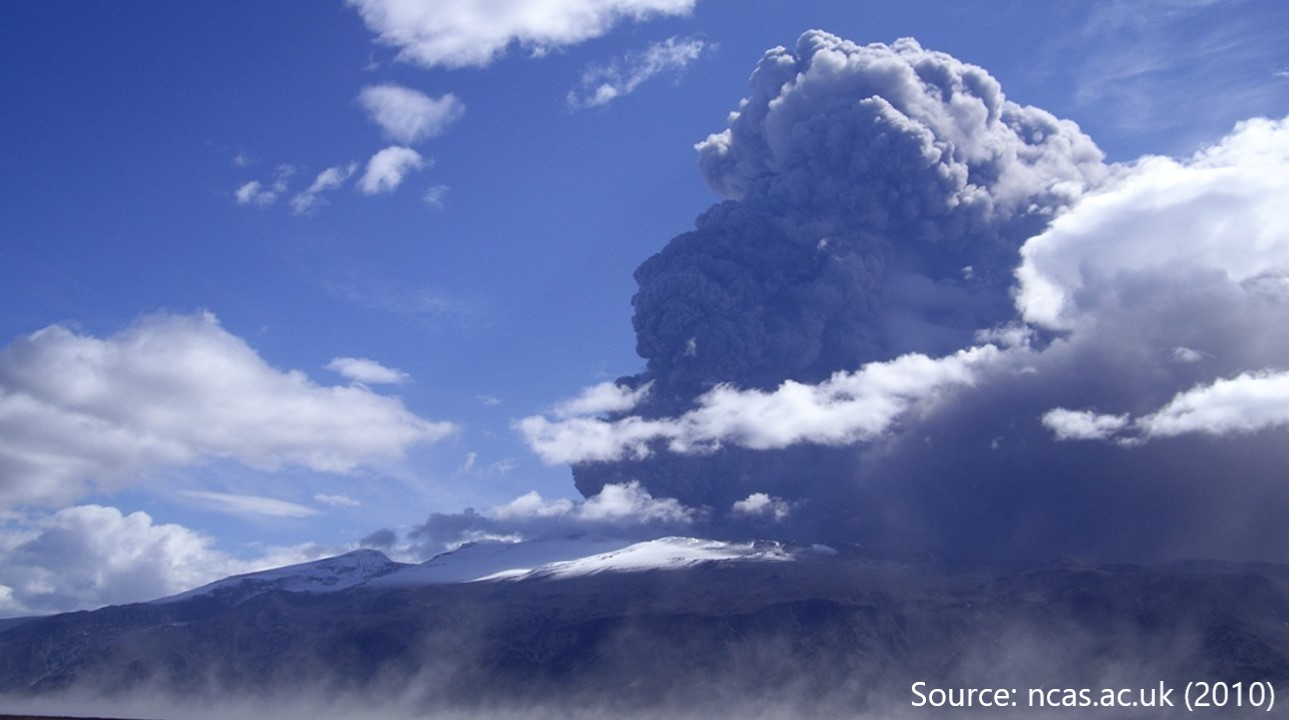
\includegraphics[width=1\textwidth]{eyjafjallajokull}
			\caption[Eruption from peaks of Eyjafjallajökull]{Eruption from peaks of Eyjafjallajökull - 2010. (Source ncas.ac.uk - 2010)}
			\label{fig:intro-eyjafjallajokull}
		\end{figure}
	
		\subsection{Northeast power outage in USA}
		In August of 2003, the northeastern part of USA faced a historical power outage, which affected 50 million consumers \cite{schewe2004}. The cause turned out to be no actual failure but an insignificant software bug that triggered a fail-safe alarm. The blackout would last two days in New York, New Jersey, Massachusetts, Michigan, and Ohio in USA, and in Ottawa and Toronto in Canada and the power disruption caused economic disturbance on a huge scale (see Figure \ref{fig:intro-northamerica-blackout}).
		
		\begin{figure}[h]
			\centering
			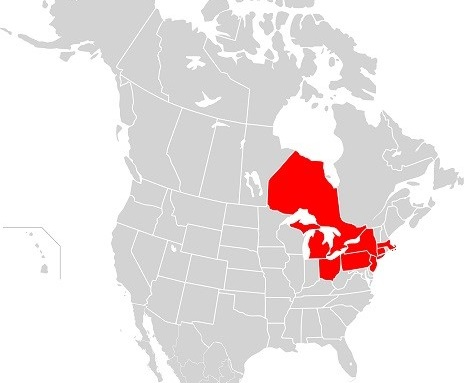
\includegraphics[width=1\textwidth]{northamerica-blackout}
			\caption[Northeast power outage]{Approximate area affected due to Northeast area power outage in 2003 (Source: Wikipedia - Lokal\_Profil).}
			\label{fig:intro-northamerica-blackout}
		\end{figure}

		\subsection{Suez canal blockage}
		In a recent incident, a 200 ton-heavy cargo vessel named Evergreen jammed in a small pass of Suez Canal, causing major disruption in global supplies of oil and other goods (See Figure \ref{fig:intro-evergreen-blockage}). The consequent financial loss incurred to the trade industry was estimated to be 400 million USD per hour for 6 days \footnote{Source: https://www.foxbusiness.com/markets/white-house-eyes-suez-canal-energy-impact}. In the global network of transport, the Suez canal is a tiny route but its significance is much higher than a majority of other channels in the world.
	
		\begin{figure}[H]
			\centering
			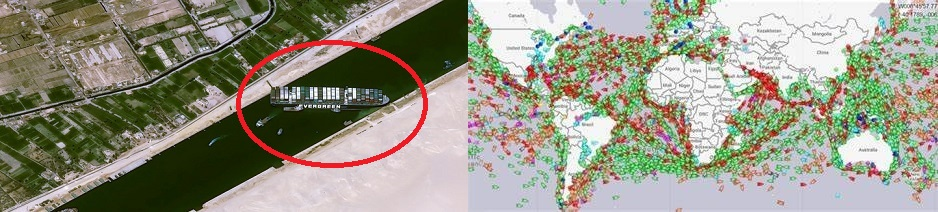
\includegraphics[width=1\textwidth]{evergreen-blockage}
			\caption[Suez canal accident]{Satellite image of Suez canal. On the left showing cargo ship Evergreen stuck in Suez canal in Egypt. The map on the right shows transport ships and freights during the time of the incident (source: FinTechNews.org - 2021). \textit{The colored version shows red spots as all the ships which were affected by the incident}.}
			\label{fig:intro-evergreen-blockage}
		\end{figure}
	
		\subsection{COVID-19 and Patient 31}
		Another interested case comes from public health sector in South Korea. In February 15th, 2020 a 60 year-old patient suffering from novel coronavirus (COVID-19) registered in a health facility in Daegu (150 miles from Seoul, the capital). Having contracted the virus, she continued her visits to a church and a restaurant, thus spreading the disease to other people. By the end of February, her visited church became a disease hot-spot\footnote{Source: https://www.thesun.co.uk/news/11553406/south-korea-patient-31-nhs-track-trace-app}. The magnitude of the spread by this patient alone can be seen in figure \ref{fig:intro-patient-31}.

		\begin{figure}[H]
			\centering
			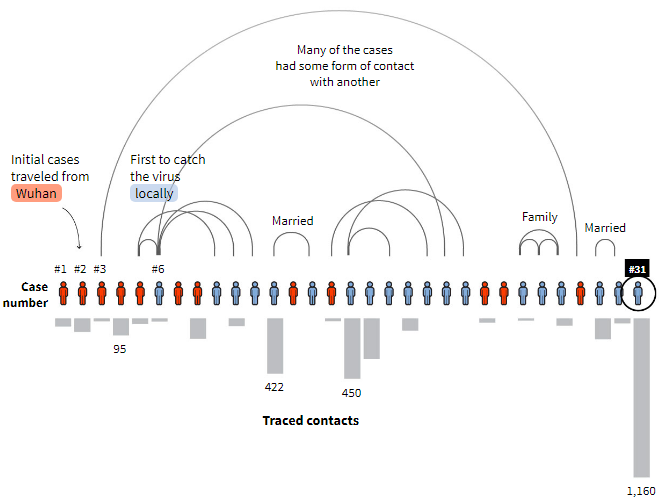
\includegraphics[width=1\textwidth]{patient-31}
			\caption[COVID19 spread in Korea]{Contact tracing graph showing how the novel coronavirus spread from original source in Wuhan to patient 31 (source: Reuters - 2020).}
			\label{fig:intro-patient-31}
		\end{figure}

From the above-discussed case studies, we observe that there are some people, places, or events that seemingly appear insignificant but leave a huge impact on real-world systems. This research is about studying connected systems and relevant methods to identify these impactful people, places, or events. Typically, this entails a small set of individual entities which can effectively spread an action, be it to deliver a piece of breaking news in a social network, market a product to a network of multinational businesses, or place sensors in a sea bed to detect rare species in most probable paths in a network of deep-sea junctions. And this can be done using what this document refers to as \textit{Influence Mining} \footnote{The term "influence mining" was first used by Liu et. al. in 2010\cite{liu2010}}.

Next sections shed light on what networks are and how they can be used to solve the outstanding problem of influence mining.

	\section{What are networks? How can they be used for influence mining?}
	\label{sec:intro-networks}
	Consider a food web\footnote{Ecological food cycle order, which defines what-eats-what.} \cite{cohen1990}, a network of neurons in the brain of a worm \cite{achacoso1991}, global airline routes \cite{guimera2005}, or the World Wide Web \cite{www2015}, all of these unified and connected systems can be represented using Graph theory\footnote{A branch of mathematics, which deals with interactions (edges) between two or more objects (nodes).} in a very simple manner. Each entity can be considered a Node and each interaction between two of such entities can be considered an edge. This formation is generalizable to many domains with numerous applications. Figure \ref{fig:intro-evergreen-blockage} is an example, where the Suez canal is a highly influential edge. Similarly, figure \ref{fig:intro-patient-31} is an example where patient 31 is a highly influential person in the network of her contacts.
	%, and can also be easily scaled.
	
	Graphs or -- referred to from here on as -- Networks are of various types. Regular networks are mathematically constructed and follow a fixed pattern. These networks have lowest heterogeneity (the number of connections each node has are quite uniform) as well as low randomness (meaning that the probability of two nodes to be connected follow a fixed pattern). Some examples of regular networks are:
	
	\begin{enumerate}
		\item Binary trees: A network in which each node has either one or two child nodes. %TODO: Add reference
		
		\item Mesh: Also called grid, is a network in which is graph cartesian product of path graphs on $m$ and $n$ nodes. It is expressed visually as a grid of $n$ rows and $m$ columns. %TODO: Add reference
		
		\item N-regular: A network in which each node has exactly $n$ neighbours, i.e. the degree is same for all nodes. %TODO: Add reference
		
		\item Clique: A type of network in which every node has a direct edge with every other node in the network. %TODO: Add reference
	\end{enumerate}
	
	 Examples of regular networks can be found frequently in engineering, similar to how a computer network can have a star schema in which one node is connected with every other node, forming a star shape. Another example can be a ring of train stations in which each node is connected to exactly two nodes to form a circle. Figure \ref{fig:intro-regular-graphs} shows some examples of regular graphs.
		
	\begin{figure}
		\subfloat[Binary tree]{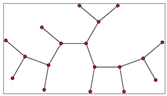
\includegraphics[width=0.3\textwidth]{graph_binary_tree}}
		\subfloat[Mesh graph]{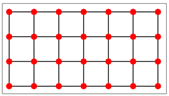
\includegraphics[width=0.3\textwidth]{graph_mesh}}
		\subfloat[$n$-regular graph]{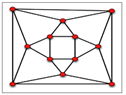
\includegraphics[width=0.3\textwidth]{graph_n_regular}}
		\caption[Examples of regular graphs]{Various types of regular graphs. Each of these are following a fixed pattern of connections.}
		\label{fig:intro-regular-graphs}
	\end{figure}

	Second type of networks are random networks. They are identified by their key property that the probability of connection between any two nodes follows random distribution. Such networks are only generated synthetically, they do not exist in real-world. Famous scientist Albert-László Barabási said:
	
	\textit{We do not know of any real network that is accurately described by the random network model.}\cite{barabasi2016}
	
	However, random networks play a key role in theoretical studies around connected systems. They also provide benchmarks for comparison when real world connected systems are studied for various phenomena.
	
	% They also serve the purpose of starter graphs in order to construct other complex networks \cite{zaidi2013}.
	
	The third type is called Complex networks. In contrast to regular networks, complex networks are highly heterogeneous and have high randomness. The Pareto principal does not apply on regular or random networks because each node in those networks is similar in properties to other nodes; instead, it applies to complex networks where nodes differ from each other in one or more ways.
	
	Complex networks themselves are a broad group, and contain further different types of networks, and because of their relationship with real life scenarios, the area of complex network analysis has caught attention in the last few decades. From neural networks in a human brain to a social network of professionals, an Intranet of computers to Internet of things, and network of food delivery riders to global networks of airways, the applications where complex networks can be found are limitless. The examples given in \ref{sec:intro-global-events} are a few cases of complex networks: the Iceland volcano eruption is a case based on a network of airways; the Suez canal blockage is an example from global sea trade industry; patient 31 is a case from a contact tracing network in epidemiology.
	
	It is not trivial to study complex networks in a generic view, they are studied on at least three levels: micro-scale, which focuses on individual nodes; meso-scale, an intermediate level which deals with entities like clusters and groups; macro-scale, where the network is analyzed as a whole. As a result, such networks hold some properties for which, conventional techniques of studying them are no longer applicable; this opens new gates of exploration for us. Some commonly observed examples include scale free structure \cite{barabasi1999}, in which the degree distribution of the nodes follow Power-law (as shown in figure \ref{fig:intro-scale-free-network}; small-world property \cite{watts1998} in which the nodes have high number of triads\footnote{A complete graph of three nodes in a network.} and small average path length (APL)\footnote{Average minimum number of edges required to travel from one node to the other.} (figure \ref{fig:intro-small-world-network} is an example); community structure \cite{strogatz2001} where cluster-like sub-networks can be observed within a large network; high tolerance (resilience) \cite{albert2004}, where the network does not collapse or change its structure if a few random nodes are removed. These three levels are not completely segregated, they overlap each other. Thus it is vital to analyze a complex network holistically as well as on granular scale.
	

	\begin{figure}[H]
		\centering
		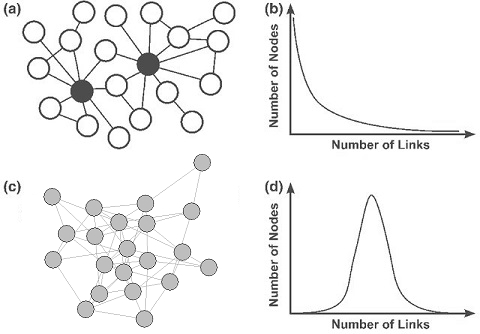
\includegraphics[width=0.75\textwidth]{scale-free-network}
		\caption[Scale free network]{Diagram 'a' shows a scale free network with some vital nodes highlighted; diagram 'b' shows the distribution of node degrees of the scale free network; diagram 'c' is a random network; diagram 'd' is the distribution of node degrees of the random network (attribution: Ilya-Temkin - ResearchGate.com).}
		\label{fig:intro-scale-free-network}
	\end{figure}
	
	\begin{figure}[H]
		\centering
		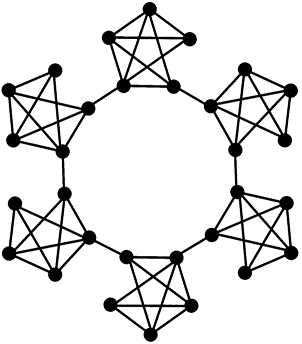
\includegraphics[width=0.5\textwidth]{small-world-network}
		\caption[Small-world network]{Watts and Strogatz model of small-world networks. Given example is generated by rewiring a lattice (regular network).}
		\label{fig:intro-small-world-network}
	\end{figure}
	
	Some advanced types of complex networks also include heterogeneous networks in which nodes and/or edges can be of multiple types (see figure \ref{fig:intro-heterogeneous-network}, and evolving networks which change their shape over time like the one shown in figure \ref{fig:intro-evolving-network}. The aforementioned examples only scratch the surface. The stack of known complex network types is thick, Costa et. al \cite{costa2011} thoroughly discussed a variety of complex networks and their applications in 22 ways. As specified in \ref{chp:domain}, it is beyond the scope of this study to discuss each type of complex network.
	
	\begin{figure}[H]
		\centering
		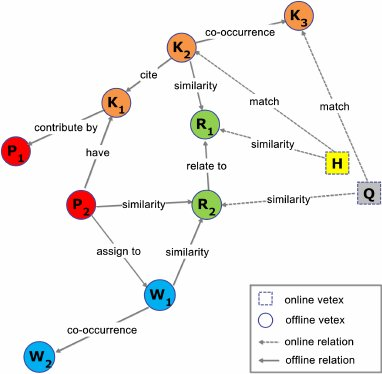
\includegraphics[width=0.5\textwidth]{heterogeneous-network}
		\caption[Heterogeneous network (OER)]{Heterogeneous network of Open Educational Resource based collaboration (attribution: Xiaozhong Liu \cite{liu2015b}). There are two types of nodes, online and offline as well as two types of relationships, i.e. online and offline.}
		\label{fig:intro-heterogeneous-network}
	\end{figure}
	
	\begin{figure}[H]
		\centering
		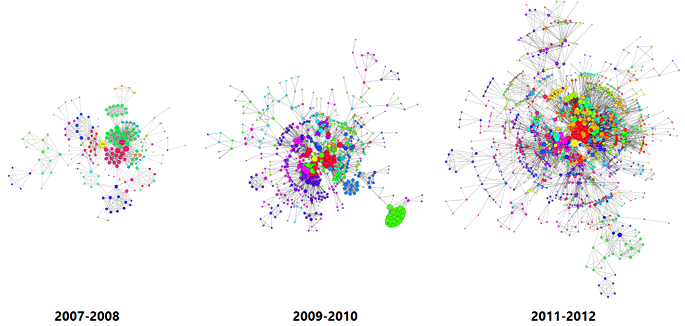
\includegraphics[width=1\textwidth]{evolving-network}
		\caption[Evolving network of Apple Inc.]{Inventor network of Apple Inc. Each node is an inventor, and an edge shows a collaboration of a patented invention.}
		\label{fig:intro-evolving-network}
	\end{figure}


	\section{Social networks: a use case of complex networks}
	\label{sec:intro-social-networks}
	Among all common complex networks, social networks are very well studied across a spectrum, ranging from a handful of students to the largest network of social ties in the 21st century, Facebook – connecting over 1 billion people. Social networks exhibit the properties of complex networks, i.e. they are scale free as well as small-world, contain community structures, are heterogeneous, and exhibit more unique properties than any other class of network. A social network may consist of following components, which shall be discussed later as required:
	
	\begin{itemize}
		\item Platforms including Social Networking, Blogging/Micro-blogging, Content Sharing, Message Boards, Chat Rooms, Podcasts, RSS Feed and Web Widget \cite{cui2011}.
		
		\item Active participants. These are typically the nodes in social network.
		
		\item Information generated and shared between users. This information is in form of transaction logs, a term used by researchers; such logs are usually in form of structured database, not in a graph form.
		
		\item Relations between users like Friend, Family, Co-worker, Acquaintance, etc. These relations are represented as edges in the social network. Some researchers have used the term "link" instead of "edge".
	\end{itemize}
	
	Thus, a prime example of complex network analysis is studying correlation \footnote{Discovering patterns by analyzing actions performed by pairs of nodes in a network.} between nodes in a large social network, in which people are connected to each other in various manners, making it harder to understand the nature and the cause of relationship between them. To understand this concept better, imagine five customers shopping for a flower pot in a nursery. First customer buys a lavender plant; of the rest of the customers, three more also buy a lavender pot. How did this happen? If we rule out coincidence, then the logical conclusion would be that there is some kind of \textit{correlation} in buying patterns between these four customers, which does not match with the fifth customer. From here, we can draw three conclusions:
	
	\begin{enumerate}
		\item All four customers like scent and colour of lavender flower, and bought them out of their own liking. In this case, the correlation is their personal preference.
		
		\item They live in same neighbourhood where mosquito are common, and lavender scent is a good repellent of mosquito. Therefore, they did not buy due to personal liking but rather the correlation between their purchase were confounding factors.
		
		\item The first customer inspired other customers to buy the same plant. In this case, neither personal preference nor confounding factors were involved. Such source of correlation is called influence.
	\end{enumerate}
	
	Anagnostopoulos has explained these correlation sources in detail \cite{anagnostopoulos2008}. In the same fashion -- as the use case of social networks -- an example from complex networks can be transportation networks, where the airports/sea ports can be considered as nodes and direct flights/sea routes between them can be edges. This network grows as newer logistic corridors are formed between countries, shaping into a complex network. Recalling from example of Suez canal blockage, the network shown in figure \ref{fig:intro-evergreen-blockage} illustrates the tens of thousands of cargo ships sailing from one port to another, the ports in this case are nodes while the route these ships follow are edges. Ports can be connected with each other either directly, or via a path. The objective of discovering influential nodes in such networks is fundamentally similar to social networks \cite{rocha2017}. \\
	
	\section{Application areas}
	\label{sec:intro-applications}
	The spectrum of applications of influence mining is broad. A holistic method to describe several application areas will be that any problem which can be mathematically modeled as a graph such that the nodes of the graph describe entities and edges define the relationships between these entities, and that the objective of the problem is to identify vital or influential entities and/or super spreaders which have the potential to impact other entities and their relationships, can be studied as a use case of influence mining. We further discuss a few application areas as follows:
	
		\subsection{Viral marketing}
		One of the widest applications of social influence is in the field of viral marketing. The concept behind viral marketing is to promote an idea, a product or news in a network of people by finding influential nodes; this way, with a minimal marketing cost, the marketing objectives can be achieved, i.e. spreading the idea, product to a large part of a social network \cite{tang2017,talukder2018}.

		\subsection{Outbreak detection}
		Outbreak detection is selecting nodes in a network to detect and prevent the spread of a virus or malware in order to minimize damages. This is another application with wider reach as it can be applied to many domains where an event can cause a ripple effect mutilating an entire network \cite{balthrop2004}. The examples of Northeast power outage and Patient 31 of COVID19 virus discussed in section \ref{sec:intro-global-events} are both cases of outbreak detection.
		
		\subsection{Recommender systems}
		Online social networks have become very popular in the past few years with billions of visitors each day. There are various applications of influence maximization in social networks such as Twitter and Facebook \cite{banerjee2020}. For example, application of recommendation systems in which the goal is to recommend the right products and utilities to a user based on the transaction log of his close network \cite{cai2020}, who are likely to influence this user to buy those products. Such applications require high-quality data on various personality traits, locale details and transaction trails. Moreover, due to growing concerns on information privacy \cite{kayes2017}, it is becoming harder to collect and keep user data. With the help of influence mining, such challenges can be overcome as the data requirements are reduced to network information and transaction logs.
		
		\subsection{Economy}
		Financial markets, especially with the emerging boom of crypto-currencies, which in principal, are based on block chain networks make full use of influence mining. For example, a block chain has two types of nodes: full and partial. Partial nodes are light nodes which carry only a proportion of transaction logs, however s complete ledger is maintained on each of the Full nodes, which is not only responsible for keeping all data \footnote{As of November 2021, the ledger size of crypto-currency block chain has grown to 366GB in size. Source: https://www.blockchain.com/charts/blocks-size}, but also verify all the \textit{blocks} (a collection of verified transactions). This entails high costs of computation power, electricity consumption, and personnel to manage. The more such full nodes are added to block chain, the more time it takes to verify blocks. Influence mining can be particularly handy to identify the minimal set of full nodes to keep the block chain efficient as well as robust. In fact, it can be argued that since financial data is more reliable and accurate as compared to other fields \cite{costa2011}, influence mining is likely to be more effective if we model their instruments, business ties, investors, consumers, etc. as a network. Chapter \ref{chp:inf-max} presents an experiment on a real economic network as a case study of influence mining application. \\
	
	Moreover, the influence mining can be applied in the field of Epidemiology, especially public health for example to control a contagious disease; in Electronics to optimize a large circuit; in ecology to learn predator-pray relationships; in neuroscience to monitor the activity of brain receptors during various events; in tourism to determine the most favorable paths and destinations in order to provide best tour packages. Numerous other application areas can identified thus making this a very interesting field of study.


	\section{Why influence mining?}
	We have presented several examples from the real life where identifying influential nodes in a network can be very useful. The crucial question here is to answer whether influence mining is the right approach or not?
	
	Let us pick the first examples we discussed in section \ref{sec:intro-global-events}. The volcano eruptions from Eyjafjallajökull peak caused giant cloud of smoke and ash, thus resulting in blocking all flights routed to not only Iceland, but also through Greenland. For most of these flights, the desired destination was neither Iceland, nor Greenland but rather USA and Canada. However, due to convenience of flying near land, many of the flights transit through Iceland. The map in figure\ref{fig:europe-iceland-flights} shows that there's only one airport, i.e. Iceland's Keflavik airport, which was a destination to more than 50 flights. All the other airports seem to be less relevant. The process of influence mining would have predicted not only Keflavik, but other potential influential routes for airways, which could have been used as alternate paths in case of unavailability of Keflavik.
	
	\begin{figure}[h]
		\centering
		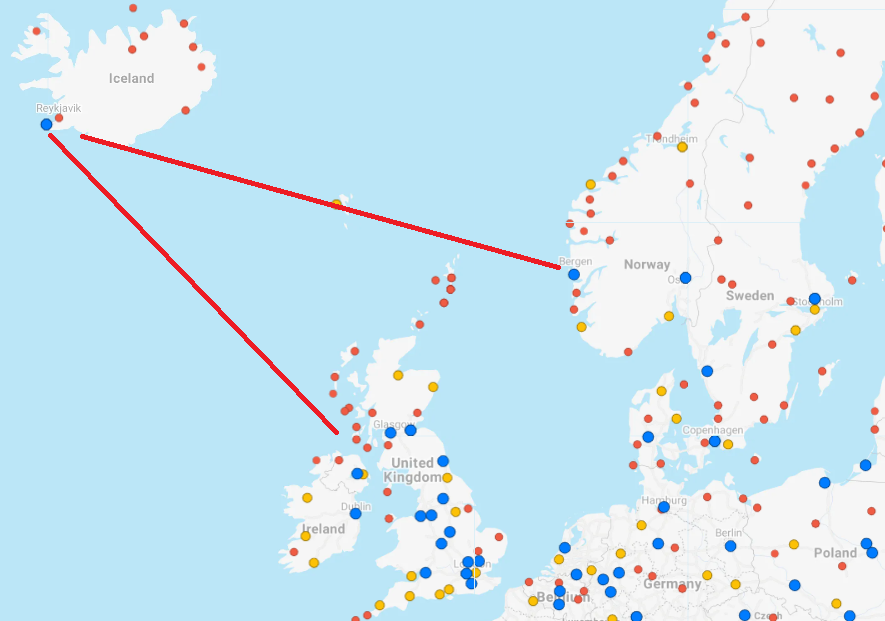
\includegraphics[width=1\textwidth]{europe-iceland-flights}
		\caption[Europe to Iceland flights]{Snapshot of European airports showing destinations. Large (blue) pins are the airports where more than 50 flights land, while small (red) circles are the airports hosting 10 or less flights (Source Flight connections - 2021).}
		\label{fig:europe-iceland-flights}
	\end{figure}
	
	Similarly, in case of Coronavirus spread from Patient number 31, the strategy of disease outbreak control followed standard contact tracing practices, i.e. start with the infected person, then trace the close contacts within 1-degree \footnote{Degree of a node is the measure of edges or links with other nodes in a network.} distance, then follow the contacts within 2-degree distances. This approach of disease transmission analysis and control is exponential and very soon makes it impossible to screen all the susceptible people. On the other hand, influence mining solution inputs a network and identifies all potential spreaders at once, thus minimizing the screening effort as well as enhancing efficiency of field workers. With application of such strategy, Patient 31 could have been identified as potential spreader much earlier \cite{dong2020}. \\

Concisely, the problem of analyzing complex network such as social networks, can therefore also be studied as a case of influence mining, which is the process of finding a set of people, places and events in a network which can independently as well as collectively influence rest of the nodes in a network to perform certain action, or respond to an action. It's important to note that there are multiple terms used in the literature to represent the same notions: "influential nodes" are also referred to as "vital nodes","super spreaders", "important nodes" or "critical nodes"; the problem of "influence mining" is originally called "influence maximization" \cite{kempe2003}, "nodes" are known as "vertices" in some studies, "edges" can also be termed as "links" or "relations". However in the next chapter we will discuss why the term "mining" is connected with the presented work, and is therefore preferred in this document.

    
    \chapter{Domain, Background and Problem Definition}
\label{chp:domain}

The problem of influence maximization starts with a set of nodes called \textit{seed}, this selection is either random, optimal, or based on certain heuristic \footnote{A problem solving method which may not provide optimal results, but are capable of producing close to the desired results.}. Each node in the seed is pre-activated, i.e. they are classified as nodes which have performed certain activity, or are already influenced by some phenomena. Then a process is simulated in which the seed nodes attempt to influence other nodes in their neighborhood to perform that same activity. This attempt is either successful or unsuccessful based on certain probability; if it turns out to be successful then the newly activated nodes also become active and repeat the same action of influencing their neighbors subsequently. Thus, a ripple effect is created which reaches and possibly influences all the nodes in a network. The main objective of influence maximization is to find out exactly which nodes are likely to maximize the spread, i.e. cause most nodes to become active.

	\section{Problem definition}
	\label{sec:domain-problem}
	In the introduction of chapter \ref{chp:intro} discusses the origin of the concept of influence with an example from social networks. In a social network, people are connected, which are described by the research community as "correlation". This correlation can be of three different types:
	
	\begin{itemize}
		\item Homophily: tendency of individuals to choose friends with similar characteristics \cite{mcpherson2001}.
		
		\item Confounding factors: external inspiration from the surrounding elements, or the environment.
		
		\item Influence: phenomenon that the action of individuals can induce their friends to act in similar way.
	\end{itemize}
	
	These correlations can be found by analyzing the structure of a network, as well as event logs of users, containing their \textit{actions}. An action is any activity performed by an individual, e.g. purchasing an item, sharing a link, tagging a photo, etc. Once an action is performed, the user performing it becomes \textit{active}. This means that if two users $u$ and $v$ are connected, then their property of being active is correlated with each other.
	
	Mathematically, if we have an undirected graph $G=(V,E)$ with nodes $V$ representing users and edges $E$ representing relation (optionally, their labels can refer to actions), then in a series of time stamps, each non-active node in $U={u_1,u_2,u_3\ldots}$ has a probability of being active, defined by probability function $p(x)\in [0,1]$. Here, $x$ is the number of active nodes in $V={v_1,v_2,v_3\ldots}$ with which the non-active node has an edge. Thus, the probability is dependent on active nodes in the connected neighbours.
	
	It is important to add that of the three stated sources of correlation, Influence is the only one which is not only correlation but causation \cite{mcpherson2001}. This has been proven by Anagnostopoulos et al. \cite{anagnostopoulos2008}. In their work, the authors did two experiments: \textit{Shuffle Test} and \textit{Edge Reversal Test}. In the first test, they proved a postulate that if the source of correlation is other than social influence, then shuffling of time steps does not affect user actions considerably. In their second test, they showed that since influence is unidirectional, then reverting the directions of edges will make significant change in propagation if the source of correlation is influence.
	
	The influence maximization (IM) problem is solved by the accurate selection of seed nodes, which are at the micro-level of a network. However it is imminent to know that a network can be studied on three scales and each scale is an important contributor when understanding a network. The next section describes these scales and comments on various properties, which are used in our experiments.
	
	
	\section{Macro-scale: structural properties of networks}
	\label{sec:domain-macro-scale}
	Structural properties are holistic level attributes of a network which explain the overall structure of a network. These properties help in classifying a network (e.g. scale-free, small-world, synchronized, etc.). Such properties have been extensively studied in past few decades and researchers have prescribed several ways to examine network structures, each method with its own significance:

	\begin{enumerate}
		%TODO: Find a book on graph theory and cite it whenver a new term is introduced in the document.
		
		\item Format: defines whether a network is directed or undirected. A directed network assumes that edges are unidirectional vectors between nodes. A directed edge from node $u$ to $v$ strictly means that $u$ is connected to $v$, it does not say $v$ is also connected to $u$. In case of undirected networks, edges are bidirectional. In our experiments, all graphs are of undirected format.		
		
		\item Weight: in a weighted network, each edge carries certain numeric value describing the significance of that particular edge. Weight can be certain probability, frequency, or other measure. If all edges have uniform weight in a network, it is considered as unweighted.
		
		\item Size (nodes): the number of total nodes in the network. The size of the network is primary metric which defines the scale.
		
		\item Edges: the number of links between nodes in the network. The greater number of edges make a graph dense and provides more channels for information to flow from one node to another.
		
		\item Average Degree: arithmetic mean of the number of edges per node in a network. Higher average degree indicates one of two things, i.e. either a big proportion of nodes are densely connected, or there exist some outlier hub nodes which are highly connected. A network with low Average Degree is not necessarily weak.
		
		\item Highest Degree: the maximum number of edges a particular node has in the network. It's sometimes denoted with $\Delta(G)$. Naturally lowest degree is denoted with $\delta(G)$\footnote{In this document, $\delta$ is not used to represent lowest degree, instead it represents \textit{gain} as discussed in \ref{chp:proof}}. However, lowest degree is majorly ignored as in almost every complex network, $\delta(G)=1$.
				
		\item Assortativity: Pearson correlation coefficient of nodes at any side of an edge. Ranging between -1 and 1, negative value means that the high degree nodes tend to connect with low degree nodes, positive value means that the nodes connect with respect to degree similarity.
		
		\item Triad Count: number of 3 interconnected nodes. Also referred as Triangles, this structural property is quite significant in complex networks because it directly impacts the strength of a network. The higher the triad count, the stronger (resilient) a network is.
		
		\item Power-law exponent ($\alpha$): in a scale free network, power-law coefficient describes how \textit{skewed} the curve in the degree-distribution plot is. Generally, this value varies between 2-3 for majority of social networks.
		
		\item Average Path Length (APL): the average minumum number of edges between shortest paths among nodes, given as $l\dfrac{1}{n(n-1)}\sum_{i,j}d_{i,j}$ where $i,j$ is any pair of nodes, $l$ is the number of nodes in the path between $i$ and $j$ and $n$ is total number of nodes in the network. Real complex networks have low APL. For example in small-world networks, nodes are connected with every other nodes through an APL of 6 or less. %TODO: add reference to 6-degree of separation
		
		\item Clustering Coefficient (CC): ratio of number of Triads connected to a node to possible number of Triads\cite{watts1998}.
		
		\item Transitivity (Global CC): Cliqueness of a network given as $C_{global}=\dfrac{3\times |triads|}{|possible_triads|}$.
		
		%\item Wedge Count: this property was introduced much later in the field \cite{seshadhri2013}. Wedge count is the number of paths with 2 edges. In larger networks, this is useful in counting the number of triads. However, its significance in broader applications is debatable.
		
		%\item Square Count: analogous to Triad count, it is the number of 4 interconnected nodes. Its use is very limited because of high cost to compute this number on larger networks, and also because Triad count already fulfills the same need which Square count proposes.
			
		\item Diameter (longest Geodesic): number of edges in longest path that exists from two most distinct nodes. Lower value of diameter suggests that the network is in form of a large cluster. Larger values indicate sparse graph.
		
		\item Density: the ratio between existing network edges and all possible edges among nodes.
		
		\item Community: a strongly connected induced sub-graph within a network. Communities are identified using a variety of methods. Not all scale-free networks have community structure, but almost all social networks have it. Presence of community plays significant role when dealing with heterogeneous networks as well as application of divide and conquer techniques on a large scale network.
		
	\end{enumerate}
	
	In experiments presented in this document, the scope was restricted to only the most widely used attributes, which include: Size, Edges, Average Degree, APL, Diameter, Transitivity, Assortativity and $\alpha$. However, wherever necessary, other properties are also indicated to support discussions and interpretations of the experimental results.
	

	\section{Micro-scale: Node properties and seed selection methods}
	\label{sec:domain-micro-scale}
	This is the granular level of a network, where properties of individual nodes are discussed. Since in a complex network, each node has its own significance and changing a few handpicked nodes can greatly impact the whole network, therefore there are many metrics available to analyze a node significance.
	
	In the influence mining process, the target is to choose a seed set and researchers have proposed various methods to select these seed nodes, and these methods can be broadly categorized into five groups:	
	
	\begin{enumerate}
		\item Topological methods: choose the seed nodes based on the structure of a network. Some nodes are very well connected in the network whereas others are loosely connected with other nodes. This associates an inherent importance to nodes due to their own connectivity as well as the connectivity of their direct neighbors.  %a  regions of a network, while some lie in the outskirts; a few nodes occur frequently during interactions between other nodes, while there will be some which are distinct.
		
		\item Simulation based methods: perform Monte Carlo simulations \footnote{A process which is repeated many times with a random selection of data. After numerous repetitions, the scenarios which happen more frequently are obtained.} to discover influential nodes in iterative manner. They provide guarantees of effectiveness within certain approximation of the best possible solution, but often fail to scale on large data sets due to the time and space complexity.
		
		\item Sampling methods: focus on identifying seed nodes via some statistical sampling method, either in single pass or in an iterative manner. The difference is that in the single pass methods, the sample of seed nodes is drawn at once, while in the iterative method, a single node or a small set of nodes is removed and the process repeats on remaining connected network.
			
		\item Community focused methods: use a divide and conquer technique. These methods first divide the network into clusters or communities using various methods, then choose seed nodes from within these communities. This way, the seed selection process can be scaled to larger networks.

		\item Scoring methods: assign a score to each node via some scoring method and select the subset of nodes with higher scores as seed. Such methods are quite effective when used on particularly friendly types of networks which are tailor made for a specific use case. %For example, famous Pagerank algorithm \cite{pagerank1999} was designed to rank web pages.
		
	\end{enumerate}

	
	\section{Information diffusion}
	\label{sec:domain-diffusion-models}
	The idea of diffusion is rooted in Epidemics. There are people infected by a certain virus or bacteria, and people who are susceptible to being infected. Some of the infected people are recovered or cured. The first and basic model of diffusion is called SI (Susceptible-Infected) model proposed by Pastorsatorras \cite{pastor2001}. The process of influence spread is actually a diffusion of information process based on SI-model, i.e. when an event is triggered on seed nodes, how is the information about that event spread to the remaining of network. There are two foundational models to observe the information diffusion process (\cite{domingos2001,richardson2002,goldenberg2001}) which are discussed below:
	
		\subsection{Linear threshold model (LT)}
		In this model, the information flow is observed from the perspective of the recipient node, i.e. the node which is inactive and will be influenced by its neighbours. The target node will have a certain threshold. If the influence of the active neighbours exceeds the threshold, then this node will also be triggered.

		\subsection{Independent cascade model (IC)}
		In this model, the flow of information is observed from the perspective of active nodes which will influence other nodes. Each active node spreads the information to its neighbourhood independently, i.e. without considering what other active nodes are doing, or what happened in the previous iterations.
		
		\subsection{Other models}
		On the basis of the foundation models, some other variants have also caught attention in literature. A few examples are enlisted in the following:
		
		\begin{enumerate}
			\item Weighted cascade model (WC): an extension to IC model with an added feature that the probability of a seed node to make its neighbouring nodes respond to the event information. This probability is calculated using the in-degree of potential nodes \cite{kempe2003}.
			
			\item Trivalency model: chooses a uniform probability between 0.1, 0.01, 0.001; this is the probability with which an individual seed node spreads the event information to its neighbour nodes \cite{chen2010}.
			
			\item Unanimous Threshold Model: this extends the LT model and adds a very strict idea that each node is highly resistant to influence and thus its activation threshold is equal to its total degree \cite{chen2009b}.
		\end{enumerate}


	\section{Diffusion process convergence}
	\label{sec:domain-convergence}
	Convergence defines when the diffusion process stops. There is only one method to halt the diffusion process, i.e. when the seed set is identified. For example, in a network of 100 nodes if the budget $k=5$ then five node are selected as seed set through some heuristic and the diffusion process is simulated on this seed set. When the propagation stops or covers entire network, then the process is said to have converged and the total number of influenced nodes is obtained as influence quantity. This parameter is provided as input to influence process and cannot be changed once set, except as a special case of Online influence maximization \cite{lei2015}, which is because in the online process, all nodes in the network are not visited at once but rather some nodes are attempted to be influenced, and based on their feedback the next set of nodes is chosen for activation.
	

	\section{Generalized view}
	\label{sec:domain-generalized-view}
	There are various components to the influence mining problem, some of which have been discussed and more will be covered later in the discussion. While the influence mining problem is subjective and depends highly on the area of application, there are three core features which are necessary to encompass this idea as a generalized model:
	
	\begin{enumerate}
		\item Seed selection: the process of identifying a set of influential nodes $S$ using an algorithm $M$.
		
		\item Diffusion or spread: the estimated number of inactive nodes, which were influenced by the seed set after completion of simulation process; note that there can be a single trial as well as several trials in a simulation. This is denoted by $\sigma(S)$.
		
		\item Convergence: external deciding factor which quantifies the information diffusion or influence, and halts the process. Typically, when all nodes in the seed nodes stop spreading the influence further, the influence process is said to be converged with an output parameter $\sigma$, which is the measure of influence spread.
	\end{enumerate}


	\section{Synthetic networks. Why are they used?}
	\label{sec:domain-synthetic-nets}
	The field of Influence Maximization uses real-world networks for real-world applications unsurprisingly. Therefore the basic optics suggests to use real networks for influence maximization experiments. However, it is not always plausible to collect, synthesize and use real networks due to many reasons.
	
	For example, famous Social networking website, Facebook was reported to have 2.6 billion monthly active users in first quarter of 2020 \cite{nasdaq2020}, i.e. the network size is 2.6 billion nodes. A network this large is impossible to process in realistic time even on the most powerful data centers. Even if attempted, the time it will take to execute even the fastest influence maximization method available will be so much that the original network would have been altered in the midst.
	
	Size is not the only factor, take DBLP \footnote{Digital Bibliography \& Library Project is a German website hosting a database of over 4.8 million research articles.} as an example. The co-authorship network extracted by this database contains disconnected components, which require pre-processing in order to apply influence maximization.
	
	Third reason is uniqueness of each network. Even in social media, Facebook's network is quite different than the famous microblogging website, Twitter, as shown by Hashmi et al. \cite{hashmi2012} that not all social networks are structurally equal.
	
	To address such complications, the researchers make use of \textit{Synthetic networks}. Synthetic networks are not collected or extracted from real-world data. They are generated by providing certain algorithms with tuneable parameters. For example, random network (see \ref{chp:intro}) based on Erdös–Rényi model \cite{erdos1960} inputs two parameters: $n$ as the size of the network to generate and $p$ as the probability of edge formation between nodes. Similarly, Barabási-Albert model adds preferential attachment \footnote{Phenomenon that the nodes tend to connect with other nodes with a preference, i.e. high-degree nodes tend to form new edges with other high-degree nodes.} parameter to grow the network in discrete time steps \cite{barabasi1999}.
	
	These synthetic networks are used for multiple reasons:
	
	\begin{enumerate}
		\item Test and evaluate new network analysis methods without real-world bias.
		
		\item As default data set to compare with the graphs extracted from real-world data.  		
		\item Identify the class of a real network by matching the statistics with existing synthetic networks with known characteristics. For example if a synthetic network is drawn using Watts model \cite{watts1998}, then a real-world network which has similar clustering coefficient and short APL will indicate that the two networks are comparable.
		
		\item Construct an ideal scenario in which the network is in clean, pre-processed form. For example, if some desired experiment is meant to be run on a complete network with community structure, then a synthetic network generator can provide such data.
		
		\item In some cases, the real network data is not available, for example due to privacy concerns. Synthetic networks work as substitute in such cases.
	\end{enumerate}

Throughout this thesis, we have used both real world networks as well as synthetic networks, as and when needed during experiments.
	

	\section{Network dismantling and resilience}
	\label{sec:domain-resilience}
	The term Resilience in network sciences is understood as tendency of a network to remain intact, such that it stays functional even if some nodes are removed. The higher the resilience, the more difficult it is to dismantle the network through random and targeted attacks\footnote{A targeted attack is when one or more nodes pre-selected by the attacker are attacked in a network in order to maximize the damage.}. This term is also synonymous in computer networks, where fault tolerance is a critical subject. Sterbenz et. al. \cite{sterbenz2011} define resilience as "the ability of the network to provide desired service even when challenged by attacks, large-scale disasters, and other failures". The subject has been extensively studied in computer networks, especially in the context of Internet security but has recently caught attention in diverse applications, including mobile networks, social networks, transport networks, and more. 
	
	The problem of network dismantling coexists -- and sometimes confused -- with decycling problem. The objective is to identify and remove the nodes such that the graph becomes acyclic, thus a node is connected with other nodes in exactly one path. The resultant graph after network decycling has $n-1$ edges, and if any edge is removed then the graph breaks into two sub-graphs. Similarly, introducing a new edge between existing nodes make the graph cyclic. The matter under discussion is strictly about network dismantling, and decycling is only used as a technique to dismantle the network such as in \cite{braunstein2016}. The relation between network dismantling and resilient node identification is the constraint $k$; the objective is to find a set of $k$ most resilient nodes which, when removed, dismantle the largest component of target network to the maximum extent possible. Meaning that if there are 100 nodes in a graph and $k=5$ nodes are to be removed, then the network dismantling problem is identifying the best set of five nodes such that if they are removed, the maximum number of edges are removed.
	
	Although there seems to be a clear segregation in past literature between resilience and influence studies, we found that both are interestingly interlinked, as discussed in chapter \ref{chp:inf-framework} in detail. \\


	\section{Influence process illustration}
	A typical influence process can be seen in figure \ref{fig:influence-process} in which a network is passed as input and based on certain iterative or non-iterative algorithm a set of seed nodes is selected. These seed nodes are then tested via inflence test or resilience test and finally the influence of the seed set is returend. Additionally, a simulation is presented in discrete steps in figure \ref{fig:ic-simulation} which tells how the diffusion process takes place in Independent cascade model as an example.
	% Source diagram here: https://drive.google.com/file/d/1AMVqRqj-GDfIZuTEUTv5SPkjt5gtoe_g/view?usp=sharing
	\begin{figure}[H]
		\centering
		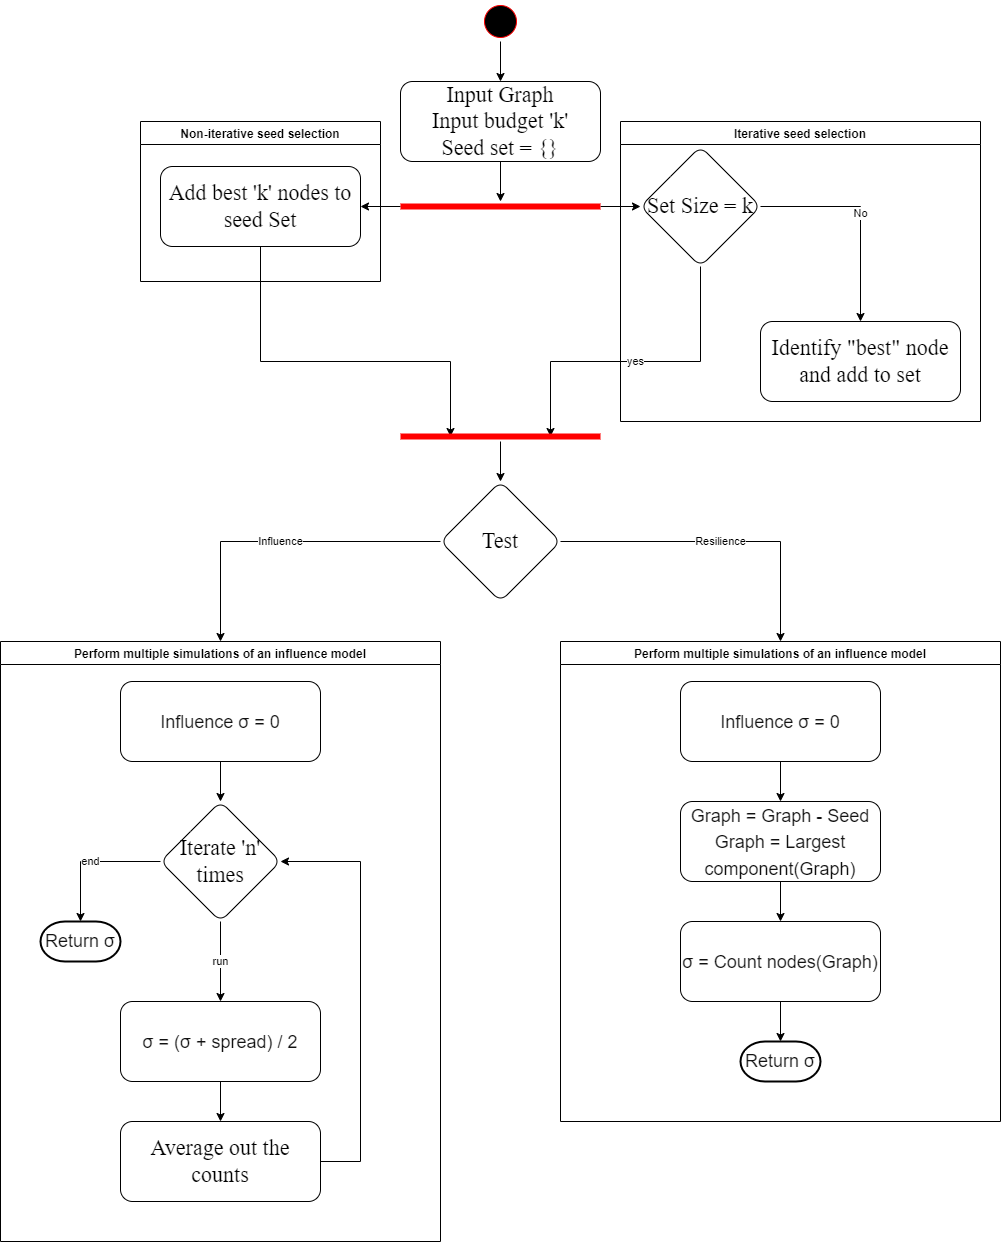
\includegraphics[width=0.7\textwidth]{influence-process}
		\caption[Influence process flow diagram]{Illustration of influence process. The function inputs a network and returns the influence measure $\sigma$ of seed nodes selected in the process.}
		\label{fig:influence-process}
	\end{figure}
	
	% Source diagram here: https://drive.google.com/file/d/1AMVqRqj-GDfIZuTEUTv5SPkjt5gtoe_g/view?usp=sharing
	\begin{figure}[H]
		\centering
		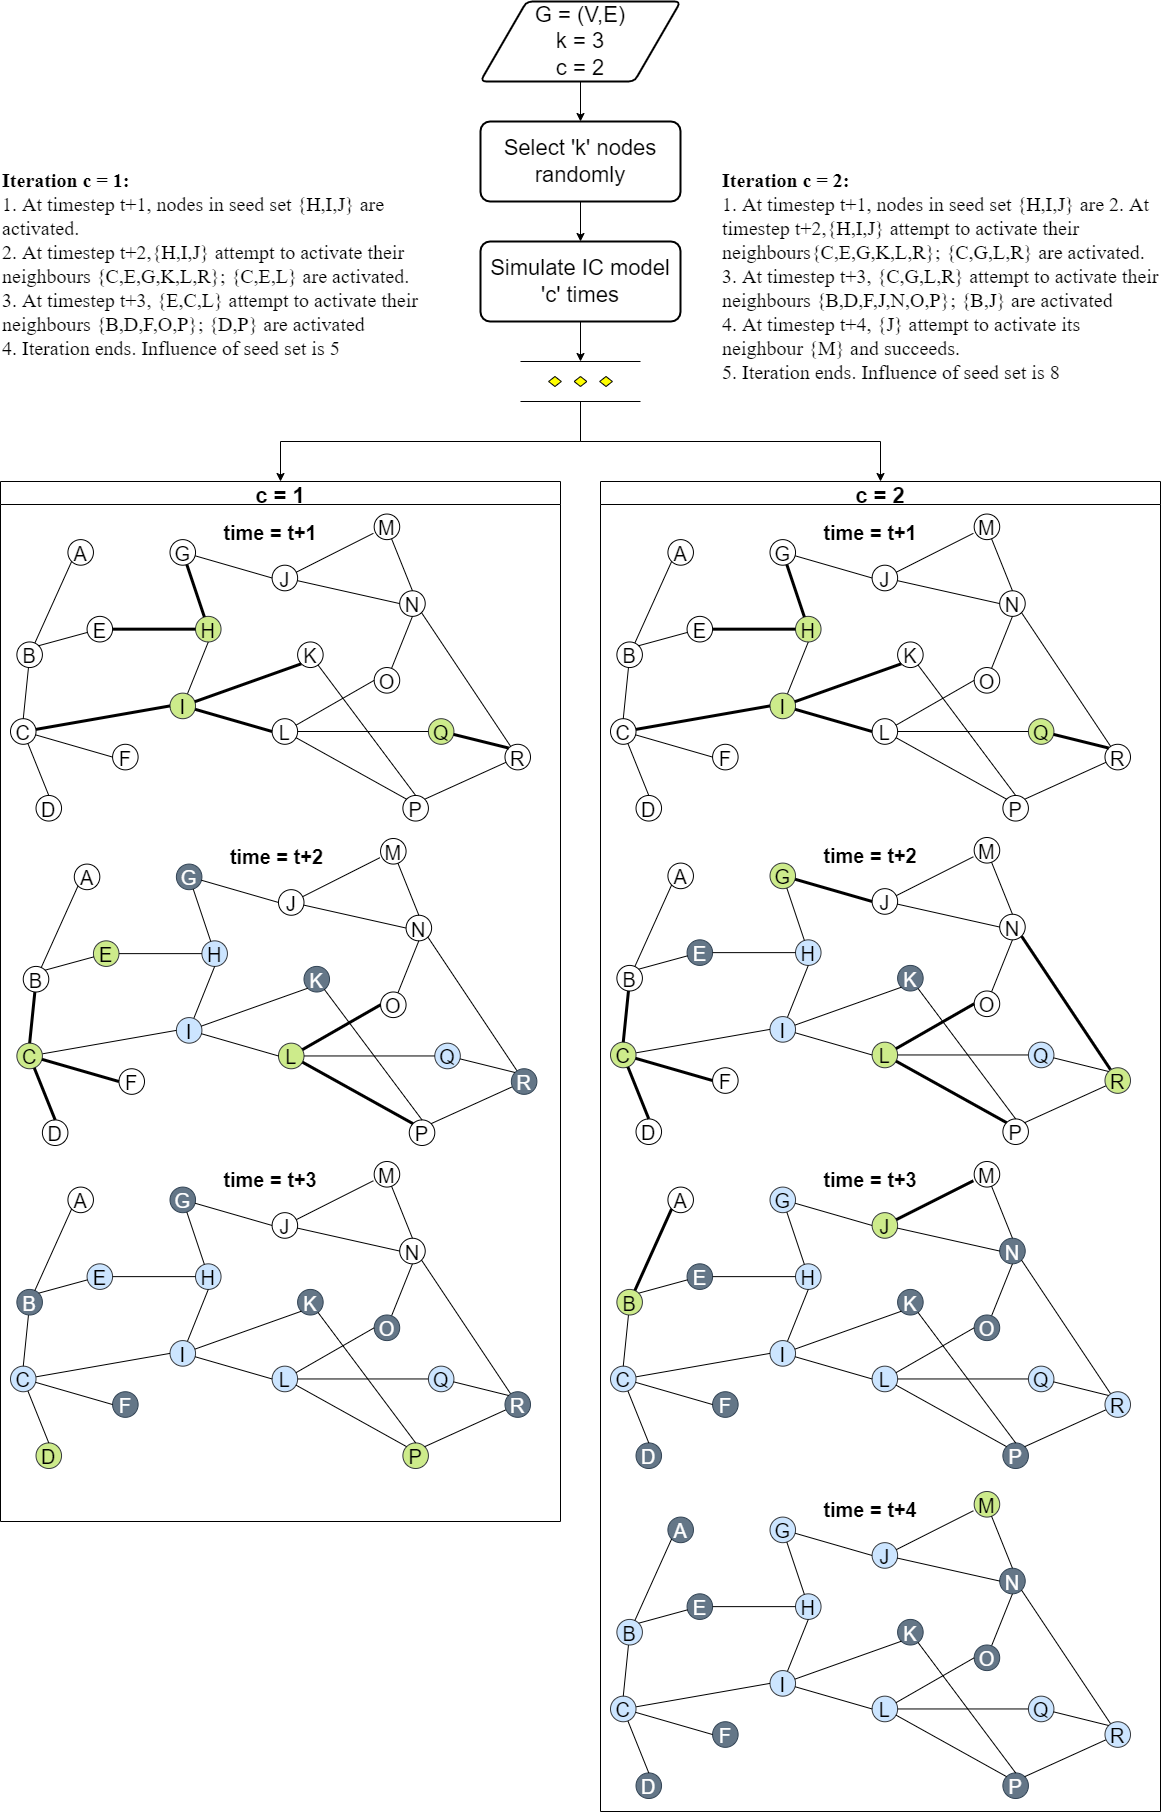
\includegraphics[width=1.0\textwidth]{ic-simulation}
		\caption[Information diffusion simulation under IC model]{An example explaining how diffusion process takes place in IC model in a graph. The two simulations shown are averaged out to give the average influence spread $\sigma$.}
		\label{fig:ic-simulation}
	\end{figure}


	\section{Summary}
	Influence maximization under any of the commonly used diffusion models is NP-hard for approximate value of spread, as given in Chapter \ref{chp:proof}; thus, these cannot be used ingenuously with real networks, because the computation time they take is too high due to the size of the network and its tendency to change dynamics rapidly, such as formation of community structure, or shortening the paths between distinct nodes, etc. Therefore, the aim should be to look for data mining approaches (such as clustering for community detection, or classification to classify nodes) for computation of influence of nodes in a complex network, so that the most influential ones can be spotted. The data mining techniques are likely to perform well because such algorithms can learn from existing state of data and adapt. For example, a straightforward approach to detect communities can be to construct fixed groups of nodes of fixed size with dense links. A data mining algorithm on the other hand will not only identify flexible sized networks, but also find hierarchies, i.e. communities within a large community. Thus this document terms the phenomenon of mining the influential nodes from a network as \textit{Influence Mining}, over the more commonly used term of Influence Maximization \cite{vahidipour1920}. \\
	
This chapter presented the fundamental concepts required to comprehend the problem of influence mining. The next chapter further capitalizes these concepts and covers the necessary details and related work in various areas.

    
	\chapter{Related work}
\label{chp:related-work}

This chapter is dedicated to a thorough review of past literature in this domain, including both classic and recent works. Section \ref{sec:related-work-areas} presents various research wings in this domain, followed by a detailed discussion on various methods of seed selection in section \ref{sec:related-seed-selection} - a key topic in influence mining. Finally, \ref{sec:related-work-resilience} spotlights works from a different community working on network dismantling; this branch is focused on the opposite dimension of the same phenomenon. Where influence mining aims to identify the best method to \textit{grow} an effect through a set of seed nodes via information diffusion, the objective of network dismantling is to identify the best method to \textit{shrink} or decompose a network. Both ideas are cut from the same fabric - identifying influential nodes.


	\section{Research areas}
	\label{sec:related-work-areas}
	Before moving to the crux of the matter, it is vital to reiterate that the influence mining domain is vast and there have been numerous studies and review conducted on the core idea.
		
		\subsection{On influence maximization}
		Domingos and Richardson \cite{domingos2001} were first to study identification of influential users and influence propagation. They model a social network as Markov Random field (an undirected graph with nodes as random variables and edges as dependencies between variables) and proposed heuristics for selection of most influential users.
		
		Extending Domingos’ work, Kempe et al. \cite{kempe2003} took greedy approximation approach to guarantee influence maximization. They focus on two basic and very frequently used diffusion models: Linear Threshold model and Independent Cascade model. In the LT model, each active neighbour $v\in V$ of an inactive neighbour $u\in V$ of network $G:(V,E)$ exerts some influence on $u$ with some probability weight $w_{v,u}$; the inactive user $u$ chooses a random uniform threshold $\theta_u$ representing minimum collective weightage required for it to be active, if $w_{v,u}\ge \theta_u$, then $u$ gets activated. The IC model says that the chance of each user $v$, which just became active on time step $t$, of influencing its inactive neighbour $u$ is independent of the past history; the probability $p_{v,u}$ is the strength of $v$ to influence $u$. Kempe et al. showed that although influence maximization problem is NP-Hard, the maximization function is submodular and monotone and therefore, we can exploit these properties to get an initial seed nearer than 63\% of the optimal set in linear time. In addition, they discuss some more tuned-up models like Triggering model, in which an inactive user $u$ independently chooses a set of active user in his neighbours that can trigger it to become active; these triggering users are the ones that genuinely can affect $u$, and then Only-Listen-Once model with efficiency within 63\%, i.e. \textit{$(1-\frac{1}{e})$} (where $e$ is the base of natural log, also called exponential constant), in which an inactive user $u$ can be activated only by one of his active neighbours. The Threshold model works on the basis of critical mass actions introduced by Granovetter \cite{granovetter1978} which proposes that an action is adopted by a person if certain number of people (or threshold) have adopted the same action; Cascade model on the other hand, is similar to SIR disease model used in epidemiology \cite{hethcote1989}, and follows the law of diminishing returns \cite{goldenberg2001}. Both of these models use timestamps of user actions; each user is either active or inactive, and the possibility of an inactive user to become active increases when its neighbouring users turn active.
	
		Chen et al. \cite{chen2010} have further extended Kempe et al. – influence maximization problem, simultaneously attacking the scalability issue of simply greedy approximation technique as well as performance lack in heuristic based solutions. %They provide a parameter to tune-up algorithms in their model, MIA (Maximum Influence Arborescence) according to the scale and performance.
		
		Watts et al. \cite{watts2007b} proposed a model called \textit{Big Seed Marketing} that reliably delivers higher marketing gain that may be achieved with any complex viral marketing model or high-budget mass marketing. Their model guarantees that a parameter called reproduction rate, $R=\beta z$ can be achieved greater than 1. Where $\beta$ is defined as the constant probability of word-of-mouth spread and represents the average of number of people that a news is spread to, by individuals.
	
		Leskovek et al. \cite{leskovec2007b} target the influence propagation problem in a different way, calling it Outbreak Detection. The problem is to detect nodes in a network, through which a virus could spread, as quickly as possible. Their work is generalized and they define influence maximization problem to be a special case of it. They developed an efficient algorithm using an approach, lazy-forward optimization\footnote{A programming technique in which instead of executing an inner function fully, a shallow function is called which returns an output from a pre-calculated heap/map.}, to select new seeds; the algorithm is 700 times more efficient than simple Greedy solution.


		\subsection{On learning influence probabilities}
		Since in the influence mining process, active nodes in the network tend to influence other inactive nodes based on certain probability, there is an open branch to identify the right probability instead of an arbitrary number. This is because not all nodes are equally influential, nor are they equally influenced, and neither is each action same in exerting influence. For example, a celebrity talking about a brand of spectacles is likely to attract people who wear spectacles; on the other hand an olympic athlete promoting a crash course on knitting is unlikely to catch as much traction.
		
		Kazumi Saito et al. \cite{saito2008} discussed how to learn influence probabilities from IC model from historical influence propagations. Their work has limitations, when applying to real-World problems, most significant of which is that their model generates initial seeds which might have less, even a single action performed, but due to larger number of neighbours, they end up being very influential nodes.
		
		There is a major outstanding problem with the existing work is that the researchers use some naïve techniques to choose probabilities associated with the edges. Like IC model assumes that the edges have uniform probabilities; WC or weighted cascade model, as proposed by Wei Chen et al. \cite{chen2010} calculate the edge probabilities between any pair of nodes $u,v$ as $p_{v,u}=\frac{1}{d^{-}_{u}}$ where $d^{-}_{u}$ is in-degree of node $u$; Trivalency model chooses a uniform probability between predefined high, medium and low (0.1, 0.01, 0.001). Kazumi Saito et al. \cite{saito2008} initially target this ignored factor by learning influence probabilities in IC model using Likelihood Maximization; they assume that propagation trace is a set of users $V$, activating in discrete time steps, but their assumption that for each inactive user $u\in V$, there must exist an active neighbour $v\in S;S\subset V$ that became active in time step $t_{u}-1$ (here, $t_u$ is the time step when node $u$ was activated), their model is more theoretical than practical. Goyal et al. \cite{goyal2011} address this by implementing different methods of learning influence probabilities using past propagation traces and compared different outcomes of greedy algorithm in IC model with naïve techniques. They divide the dataset into training data for learning influence probabilities and test data for influence maximization.
		
		In a different study \cite{goyal2010}, Goyal et al. included another aspect by showing in their experiments that the influence probabilities decay exponentially as time unfolds. They study the same process under an alternate model, the General Threshold Model. They used this model and made the probabilities decline with time. The assumption behind this is that if a user u performs an action, like tweeting, then his linked user v will either re-tweet shortly after the tweet or never. This decline of probability is observed to be exponential.

		Barbieri et. al. \cite{barbieri2014,martinvcic2017} applied the phenomenon for link prediction; Tang et. al. \cite{tang2015b} use the same for negative link prediction (e.g. dislikes); \cite{mcgee2013} predicted location of users based on their social ties; Chen et. al. in a recent study showed how social influence can be used in music recommendation systems \cite{chen2019}.
		
		\subsection{On community detection}
		Due to the complexity of the problem, some studies suggest taking divide and conquer approach to solve it. Mahmood et al. \cite{mehmood2013} contribute by devising a greedy hierarchical method to partition a social network into communities, each consisting of nodes sharing common behaviour that has been learnt by training data. Their proposed model -- unlike most of the studies -- does not pick these $k$-users (or seed) randomly or based on centrality, etc. but rather, first communities within the network are found out and then in those communities, users with highest centrality are chosen such that the total of all users chosen is $k$. The idea behind comes from an interesting study by Goyal et al. \cite{goyal2009} who articulate that in a network, there exist tribes based on some subject of interest of the members of the tribe and leaders of these tribes that are the most influential people within local tribes. This community-based influence mining has following benefits over centrality-based methods:
		
		\begin{enumerate}
			\item The selection of seed is guaranteed to be from vast area of whole network, instead of a single more coupled region where users are highly interconnected.
			
			\item The highly influential nodes are decided on the basis of attributes of communities, not globally, giving a chance to the nodes that are locally influential but may not be globally influential.
			
			\item Computation time required is divided among communities, thus, even if we use influence maximization process, the time complexity will be reduced drastically.
		\end{enumerate}
	
		The authors proposed GuruMine, a pattern mining approach \cite{goyal2009} for finding out leaders and their tribes in a network where leaders are the users with high influence and tribes are set of users being influenced by leaders over a class of actions. Their framework proposes that given:
		
		\begin{itemize}
			\item A network $G:(V,E)$ of $V$ nodes and $E$ edges.
			
			\item A set of user actions $A$ (also referred to as action log).
			
			\item Threshold parameter $\pi$ denoting maximum propagation time. %TODO: use some other symbol instead of pi
			
			\item Threshold parameter $\psi$ denoting the least value of influence of a user $u$ with respect to an action for at least $\pi$ time.
			
			\item Threshold parameter $Infl_\pi (u,a)$ as minimum influence required by user $u$ performing action $a\in A$ to qualify as leader.
			
			\item Subset $I\subseteq A$ representing a complete set of actions performed by user $u$.
			
			\item $\xi$ be the minimum number of actions required for $u$ to qualify as leader while satisfying $Infl_\pi (u,a)$\footnote{In the original paper, this notation is $\sigma$. It is changed here to avoid confusion with $\sigma$ which is defined as measure of Influence in following chapters of this menuscript.}.
		\end{itemize}
		
		 User $u$ is a leader if $|I|\geq \xi and |Infl_\pi (u,a)|\geq \psi \forall a\in I$. For example, if we choose $\pi$=5 units, $\psi$=3 units, $\sigma$=2 units, then a user $u$ is leader if within a time slot of 5 units, users reachable from $u$ perform at least 2 actions, each action performed at least in 3 time steps. The leaders can then be tribe-leaders, a stronger notion of defining leaders for a class of actions.

		The limitation with community-based approaches is that not every network has community structure or hierarchies, thus rendering divide and conquer inapplicable.		
		
		\subsection{On heterogeneous networks}
		A distinctive work by Liu et al \cite{liu2010} discussed topic-level direct and indirect influence in heterogeneous networks. Their study is divided into: topic distribution modeling and strength estimation; the strength of influence is analyzed by probability $(p_1-p_2)$, where $p_1$ is the probability of a user’s n-degree friends to be induced to perform the same action which he did and $p_2$ is the average probability of whole population to perform that same action.
		
		\subsection{On veracity}
		Some researchers scrutinize veracity of information in social networks. Goldenberg et al. \cite{goldenberg2001} focused word-of-mouth phenomenon for marketing and information propagation and discuss effect of strong and weak ties on the speed of adoptation of an idea or product. Farajtabar et al. \cite{farajtabar2015} recently presented a framework to backtrack historical data in a social network and identify source node of malicious information. Eytan Bakshy et al. \cite{bakshy2011} argued that the word-of-mouth effect is not achieved by a small number of people but a big proportion of them. Janders \cite{jenders2013} worked on distinguishing a viral event from a non-viral event on Twitter. Ma et. al questioned the very idea of popularity, arguing that viewership is a neutral event and is not the right measure of content popularity \cite{ma2013}.

		\subsection{On benchmark methods}
		Benchmarking is one of the areas rarely explored by the researchers. A recent paper by Arora et. al. \cite{arora2017} is an open critique on the influence maximization studies. This paper evaluates several algorithms using vibrant benchmarking techniques focusing on time and memory efficiency, quality and scalability of each method. The authors establish that the efficient methods miss out on quality, the ones which offer quality cannot be scaled, and that the best methods for practical cases are the ones with higher quality and time efficiency. Moreover, some of the methods presented do not guarantee approximation on both LT and IC models.
		
		
	\section{Scalability problem and seed selection heuristics}
	\label{sec:related-seed-selection}
	In attempts to find workaround for inherent scalability problems when maximizing influence in large networks, several studies proposed different heuristics to select influential nodes. A classic and comprehensive article on centrality by Freeman \cite{freeman1979} provides foundation for various heuristics to come. Goyal et al. \cite{goyal2012} presented a greedy method to select initial seed nodes such that the coverage is at least up to a given threshold in logarithmic time, while approximation guarantees are similar to that of original greedy algorithm (see \ref{alg:influence-greedy-solution}). Encountering the scalability problem again on large networks, the research community has produced heuristics and algorithms in abundance to select seed nodes:
	
		\subsection{Topological methods}
		The term \textit{topology} refers to the structural position of nodes in the graph. These methods exploit the topological value of nodes rather than sampling or simulations. A node, which lies in the core of graph tends to be highly influential as compared to the nodes which lie in the boundaries or outermost area. While the key benefit of these is their efficiency, their major drawback is lack of theoretical guarantee on quality. There are several topological methods, and different variations out of which, some are given here.
		
		\begin{enumerate}
			\item Degree Centrality: a measure of how many connections a user has. k-users with the highest degree centrality are selected with an expense of $O(|V|)$ complexity.
			
			\item Closeness: the inverse of the average length of the shortest paths of a user to all other user; closeness value is always between 0 and 1. Users with the highest closeness are selected with an expense of $O(|V|)$ complexity.
			
			\item Betweenness: a measure of shortest paths on which it exists. k-users with the highest betweenness are selected with an expense of $O(|V|)$ complexity by using a faster solution to calculate betweenness by Brandes \cite{brandes2001}.
			
			\item Eigenvector centrality \cite{bonacich1987}: a measure of influence of a user in the network by assigning relative score to a user based on the concept that connections to high-scoring users contribute more to the score of the user; this value is always between 0 and 1. k-users with the highest Eigen value are selected with an expense of $O(|V|)$ complexity.
			
			\item Subgraph centrality: measures the weighted sum of walks of various lengths from and to the node under observation \cite{estrada2005}. However, the conjecture from the authors that \textit{if a graph has identical subgraph centrality for all nodes, then the closeness and betweenness centralities are also identical for all nodes} has been disproven by \cite{stevanovic2013}.
			
			%\item No-neighbours: this method selects only the highest degree users that are not directly connected to each other to ensure that we do not have users of a specific section of the network; the additional cost is $O(\frac{k^2}{2})$.
			
			\item Coreness: a measure to describe network cohesiveness. A network $H$ is $k$-core if it is connected maximal subnetwork of original network $G$ and the degree of each node is at least $k$. Coreness of each node in $H$ is defined as $k$. The additional cost of this method is $O(|V|)$ by using algorithm proposed by Batagelj et al. \cite{batagelj2003}.
			
			\item Centrality in Community: a cluster of users - a sub-graph, which are highly connected with each other but loosely connected to users in other communities. Users are selected from each communities with highest centrality, such that their sum is equal to k. Discovering communities by calculating the leading non-negative Eigen-vector of sub-graphs \cite{newman2006b} has an additional cost of $O(|E|+|V|^2)$. There are other community detection algorithms which can be applied to extend this technique.
			
		\end{enumerate}
		
		\subsection{Simulation based Algorithms}
		These methods perform Monte Carlo simulations to discover influential nodes in iterative manner. They provide guarantees of effectiveness within certain approximation of the best possible solution, but often fail to scale on large data sets due to the time and space complexity.
		
		% Refer to Debunking the Myths of Influence Maximization: An In-Depth Benchmarking Study
		\begin{enumerate}
			\item Greedy: exploiting the monotone and sub-modular property of the influence maximization problem, a Hill climbing greedy based algorithm has been proposed by \cite{kempe2003}, which guarantees a solution within approximately 67\% of the optimal solution.
			
			\item CELF: these are extensions of the original Greedy algorithm, with same worst time complexity, but their average time complexity is up to 27 times better than the predecessor. CELF algorithm \cite{leskovec2007b} takes a lazy-forwarding approach and instead of recomputing the influence spread of every node in each iteration, it exploits the sub-modularity property and thus reuses the pre-computed marginal gain of individual nodes in each iteration during simulation.
			
			\item CELF++: \cite{goyal2011b} further optimizes the idea behind CELF and increases the efficiency by up to 55\%. This algorithm maintains a heap $Q$ such that it preserves not only the marginal gain of individual node, but also the marginal gain of each node coupled with the best node identified in prior iteration. These values are reused during the simulation to further reduce the redundant computation of influence spread.
		\end{enumerate}
		
		\subsection{Sampling Algorithms}
		\begin{enumerate}
			\item Adaptive Sampling: a variant of sampling technique presented by Lipton \cite{lipton1989}. In an iterative way, the nodes in a network are ordered by a metric (e.g. Degree centrality) and top node or a batch of nodes are removed from the network and the process is repeated on the largest connected component until the network is completely dismantled. The same technique was used for Betweenness centrality in \cite{hussain2019} for better results than Degree centrality, proving that this technique can be used as an extension of any topology-based method. 
			
			\item TIM: draws $\theta$ number samples of reverse reachable (RR) sets from a directed network. Its results outperform the then state-of-art on largest networks tested in the literature by an near optimal efficiency of $(1-\frac{1}{e}-\epsilon)$, while offering time complexity of $O((k+l).(n+m).log(\frac{n}{\epsilon^2}))$ \cite{tang2014}. The idea behind TIM is that a node $u$ is influential if it frequently appears in the samples such that it has direct edge from each node $v$ in RR samples. %TODO: Define epsilon here
			
			\item IMM: \cite{tang2015} adds statistical optimizations to TIM in estimation and improves accuracy by adding little complexity. These techniques however, have been demonstrated only on IC model. However, these results were challenged by \cite{chen2018}, but the challenging paper also suggests workarounds with minor addition to time complexity to achieve the promised results.
			
			\item StaticGreedy: fixes a long-standing issue of Hill climbing approach that it needed many MC simulations to guarantee approximation \cite{cheng2013}. This algorithm employs a simple and effective technique of MC snapshots, i.e. instead of dynamically creating snapshots during the spread simulation, a collection of network snapshot is created and all simulations are run only on that set. Thus avoiding the need for reconstructing snapshot networks as well as guarantee the accuracy on limited number of MC simulations.
			
			\item PMC: \cite{ohsaka2014} furthers the StaticGreedy on even larger networks through graph pruning, requiring even lower number of snapshots than the former. For each randomly generated graph for MC simulations, a strongly connected weighted DAC (Directed Acyclic Graph) is computed, where the weight on nodes denote the number of nodes reachable. The influence $\sigma$ is then computed for each node via averaging gain in each DAC through BFS (Breadth First Search).
			
		\end{enumerate}
		
		\subsection{Community focused Variant}
		The topological and heuristic methods used on smaller communities identified by community detection algorithms take divide and conquer approach by splitting a large graph into communities and computing influential nodes within these communities. The most notable work in this area is by Wang et. al. \cite{wang2010}, which proposed CGA-Community based greedy algorithm which detects communities in a social network through dynamic programming and uses MixedGreedy algorithm \cite{chen2009} for influence maximization simulation within these communities. He et. al. \cite{he2015} furthered the idea later by first identifying \textit{super nodes} (strongly connected communities) and then choosing one spreader node from each super node. This method improves on time complexity as well as simulates realistic community detection.
		
		The community focused variant has a pitfall that it can work only on the networks which have community structure, Social networks are best examples here. However, on sparse networks, this technique is not applicable.
		
		\subsection{Scoring Algorithms}
		This class of algorithm assigns a particular rank or score to each node and selects $k$ nodes with highest scores as seed set. Such methods are quite effective when used on particularly friendly types of networks for which their baseline technique was tailor made.
		
		\begin{enumerate}
			\item Pagerank: Brin and Page made a breakthrough in the web search engine history in 1999 \cite{pagerank1999} with their proposed web page ranking method. A web page gets higher rank if it is linked with more web pages. The same idea is applied on networks to identify influential seed nodes. If $u$ is a node to be ranked and $v\in N_u$ are all nodes directly with $u$, then the rank $R_u=c\sum_{v\in N_u}\frac{R(v)}{|N_v|}$. The algorithm is very fast with $O(|V|+2|E|)$ time complexity.
			
			\item Collective Influence: Morone et. al. \cite{morone2015} discovered that on larger networks, influential nodes are often weakly connected, and that the same influence spread can be achieved with a much smaller seed set than the other heuristics suggest. Collective influence is calculated by multiplying the degree of node $u$ with sum of all degrees of the set of its neighbouring nodes $N_u$ up to some distance $\delta$ (e.g. $\delta=1$ represents direct neighbours, $\delta=2$ represents neighbours of direct neighbours and so on). Therefore if $\Lambda_u$ denotes set of all nodes of $u$ within a distance $\delta$, then simply, $CI(u)=d_u * \sum d_{\Lambda_u}$. The running time complexity of this methods is $O(|E||V|log|V|)$.
			
			\item SIMPATH: competes directly with LDAG \cite{chen2010b} and presents the phenomenon that in LT model, the spread of a node is driven by the spread of the induced subgraph consisting of its neighbours. Mathematically, $\sigma(S)=\sum_{u\in S}\sigma(u\cup (V-S))$. This optimization significantly reduces the estimation calls. Consequently, a score is assigned to each node by summing up the probabilities all simple paths from $u$ to other nodes. The length of the simple paths are restricted through a tolerance parameter $\eta$, as computing full length paths itself is NP-hard, and useless because of the property of diminishing returns.
			
			\item EaSyIM: \cite{galhotra2016} is the state of art in the class for its low memory footprint of $O(|V|)$ and linear time complexity of $O(kD(|V|+|E|))$ where $k$ is the size of seed set and $D$ is diameter of network. The algorithm assigns EaSyIM score to each node by calculating weighted sum of number of paths of length $l$ starting from $u$, while the weight of path is the product of edge probabilities that lie on that path.
			
			\item IMRank: is a rank refinement technique on top of other scoring algorithms for IC model \cite{cheng2014b}. A scoring method is used to calculate scores in first iteration, but in the consequent steps a last-to-first reverse rank ordering method is used to improve the efficiency of marginal gain estimation. This algorithm guarantees the self-consistent ranking by calculating marginal ranking of nodes in iterations with respect to their previous rank.
			
		\end{enumerate}


	\section{Network dismantling and Resilience}
	\label{sec:related-work-resilience}
	This problem is conventionally presented as graph dismantling, which is to identify a minimal set of vertices such that removing this set disintegrates the original graph into connected sub-graphs of sizes no larger than predefined. Formally, a connected graph $G=(V,E)$ is decomposed by removing the edges in iterative manner such that there does not remain any sub-graph $H_i$ for which there exists an edge between any pair of nodes $i,j$.

		\subsection{Resilience}
		\label{subsec:related-work-resilience}
		Resilience, as described in \ref{sec:domain-resilience} is a network's ability to hold itself together when its nodes are individually under a targeted attack. The more resilient a network is, the more nodes will have to be taken down in order to dismantle the network. Latif et al. \cite{latif2014} studied network resilience under different kind of networks, their work focuses on exploiting the structure of different networks like scale-free and small-world networks and compare the resilience of these networks under different forms of attacks.
		
		Among the most basic methods are degree and other centrality based. Degree centrality is generally used alongside Random selection method for benchmarking and comparison purpose. \cite{braunstein2016} shows that Eigenvalue centrality stands out on Erdos–Rényi random graphs among other centrality heuristics while introducing their Min-Sum decycling algorithm.
		
		Apart from centrality based methods, Pagerank \cite{pagerank1999} stands out as a fast and effective baseline heuristic to identify resilient nodes. Lü et. al \cite{lu2011} introduced LeaderRank, an algorithm based on Random walk which outperformed Pagerank on directed social networks.
		
		Chen \cite{chen2012b} and others proposed a \textit{local centrality} method, which computes the centrality as sum of degrees of 2-step neighbourhood of a node \ref{eq:local-centrality}:
		
		\begin{equation}
			\label{eq:local-centrality}
			C(v)=\sum_{u\in\Gamma(v)}(\sum_{\omega\in\Gamma(u)}N(\omega))
		\end{equation}
		
		Where $\Gamma(u)$ is the set of neighbouring nodes of $u$ and $N(\omega)$ is the set of nieghbouring nodes to second degree (neighbours of neighbours). This method provides a good trade off between effectiveness which centrality based methods miss, and expensive computation time like Greedy solution.
		
		Among the most established topological methods, $k$-shell decomposition algorithm was first presented in a classic study \cite{seidman1983}. Analogous to atomic structure, the most central nodes are in the $k_{max}$ shell, then the rest of the nodes belong to one of the shells between $k_1$ and $k_{max-1}$. The nodes in $k_1$ shell are those with degree = 1. In order to identify $k_n$ shell, all the nodes with degree $n-1$ are removed in iterative manner. The $k$-shell decomposition seems to overlap with $k$-core. However the key difference is that a graph's $k$-core is the maximal subgraph in which each node has a degree $k$ or higher. On the other hand, $k$-shell is a set of nodes which are part of the subgraph $k$-core but not $(k+1)$-core. The $k$-shell methodology was used in the context of internet resilience by Carmi et. al. \cite{carmi2007} who studied the Internet map and showed that using their proposed enhancement, the Internet map can be decomposed in 6-shell decomposition.
		
		Later, Kitstak \cite{kitsak2010} propagated this method on large scale on Social networks, including one with 3.4M nodes under SIS\footnote{Susceptible-Infected-Susceptible} and SIR\footnote{Susceptible-Infected-Recovered} models of epidemiology. Their study confirms the hypothesis that it is the topology, not the connectedness of a node which decides how vital it is in the network when spreading a contagion.
		
		An argument can be made against k-shell decomposition method that it has a limitation particularly in Social networks. For example, \cite{borge2012} found out that for rumor diffusion, k-shell method is not very effective. We argue that the said method identifies the \textit{oldest} nodes as influential, while in social networks are organically built, the network takes community form and diverges into Leaders and Tribes, as shown by Goyal et. al. \cite{goyal2008}.
		

	\section{State-of-art}
	\label{sec:related-work-state-of-art}
	Among the recent work in the domain of influence mining, one of the most prominent works is by Lei \cite{lei2015}. It presents a framework of influence maximization in online mode, which has the capability of switching between Exploit mode when exact information about influence probabilities is available, and Explore mode when it the probabilities are to be calculated. The proposed model is incremental, and reuses the users’ feedback information extracted from previous iterations. Traditionally, influence maximization problems have an offline setting, in which the network is fixed and edge probabilities are known. The author redefines the problem as a weighted graph $G=(V,E,p)$ where probabilities $p_{u,v}$ (probability of node $u$ to influence node $v$) are not known; the objective is to find a seed set $S$ with $|S_n|\leq k$, which maximizes the set of edges $E[|\cup_{1\leq n \leq N}I(S_n)|]$ where $k$ is the budget consisting of $N$ trials with $1\leq k\leq |V|$, $I(S_n)$ is the set of nodes influenced in trial $n$.
	
	On community detection in networks, Fortunato \cite{fortunato2016} attack a long-open problem that there is no universally accepted protocol about defining goodness of a community detection method. The author defines three classes to assess performance of a community detection method:
	
	\begin{enumerate}
		\item Internal Connectedness: this class defines how cohisive the graph is. This measurement is calculated from three variables:
		
		\begin{itemize}
			\item Internal Degree ($k^{int}_{C}=\sum_{i,j\in C}A_{i,j}$) is sum of internal degrees of all nodes in a subgraph $C$ in the graph adjacency matrix $A$.
			
			\item Average Internal Degree ($k^{avg-int}_{C}=\frac{k^{int}_{C}}{n_C}$) is the sum of average internal degrees in $C$.
			
			\item Internal Edge Density ($\delta^{int}_{C}=\frac{k^{int}_{C}}{n_C(n_C-1)}$) is the ratio between number of internal edges and number of possible internal edges in $C$.
		\end{itemize}
		
		\item External Connectedness: in contrast to internal connectedness, this class defines how embedded the network between sub-networks. There are three main variables to check the external connectedness:
		
		\begin{itemize}
			\item External Degree ($k^{ext}_{C}=\sum_{i,j\not\in C}A_{i,j}$) is sum of external degrees of all nodes in a subgraph $C$.
			
			\item Average External Degree ($k^{avg-ext}_{C}=\frac{k^{ext}_{C}}{n_C}$) is the sum of average external degrees in $C$.
			
			\item External Edge Density ($\delta^{ext}_{C}=\frac{k^{ext}_{C}}{n_C(n-n_C)}$) is the ratio between number of external edges and number of possible external edges in $C$.
		\end{itemize}
		
		\item Hybrid Measure: this class can have plenty of examples, like:
		
		\begin{itemize}
			\item Total Degree, or Volume ($k_C=\sum_{i\in C,j}A_{i,j}$) is the sum of all degrees.
			
			\item Average Degree ($k^{avg}_{C}=\frac{k_C}{n_C}$) is the average degree of all nodes.
			
			\item Conductance ($C_c=\frac{k^{ext}_C}{k_C}$) is the ratio between external degree and total degree of $C$.
		\end{itemize}
		
	\end{enumerate}
	
	The author iterates that modern view of community detection is more probabilistic than classical view, which considers counts. In modern view, a \textit{strong community} is the one in which the nodes in a subgraph has higher link-probability than external nodes. Where in a \textit{weak community}, average link probability within a subgraph exceeds the average link-probability of nodes in the subgraph with nodes of any other group.
	
	Lü, et al. \cite{lu2011} present an empirical, yet comprehensive article on vital nodes in a network and means to extract them. Key contribution in this paper is the way several classes of vital node extraction are discussed:
	
	\begin{enumerate}
		\item Structural Centralities: this class of centralities takes into account the structural properties of nodes. Authors further categorize this class into two subclasses: Neighbourhood-based and Path-based centralities.
		
		\item Iterative Refinement Centralities: in this class, the importance of a node is determined by the importance of neighbours, iteratively. Authors discuss several methods for undirected networks like Eigenvector centrality, and directed networks like PageRank.
		
		\item Node Operation: contrary to using structural properties, this class deals with identifying targeted nodes in a network, which could be attack-sensitive with respect to connectivity, stability, or node contraction, etc.
		
		\item Dynamics-sensitivity: here, some context about the network is introduced, like time stamp. Social networks, for example, are evolving, and their dynamics are important when identifying vital nodes.
		
		\item Influence Maximization Methods: the NP-hard problem of identifying an optimal vital set of nodes in a network. There are various aspect of this problem, for example, finding out minimal set of optimal nodes; identifying a set of optimal nodes with a fixed budget; finding a set of nodes with fixed desired influence. This class is quite broad and is further broken into Structural and Functional Influence Maximization.
		
		\item Greedy Method and Heuristics: these are the most commonly observed classes, proposed as a scalable alternative to IM. Greedy method has complexity of $O(n^2)$ and guarantees accuracy within a factor $1-\frac{1}{e}\approx 0.63$ of optimal results.
	\end{enumerate}
	
	The above methods are discussed on unweighted, weighted and bipartite networks for their performance.
	
	In the area of network resilience, a notable series of experiments were conducted to further the state-of-art. Gao \cite{gao2016} et al. have studied resilience in complex networks and proposed a general analytical framework, which provides a one-dimensional view for multi-dimensional complex networks. This paper does not introduce a specific algorithm, but rather guidelines on how to design methods to depict resilience within a real-world network. 
	
	On rank-based methods, Morone, Makse and others \cite{morone2015} rejuvenate the state of art using Percolation\footnote{a classical theory which studies the interaction of particles in a random medium\cite{shante1971}}. The authors proposed optimal percolation method which determines the minimum seed set required for a structural collapse. The influential nodes are identified by calculating a Collective Influence rank with respect to certain radius $l$, i.e. $CI_l(u)=(k_u-1)\sum_{v\in H(u,l)}(k_v-1)$, where $u$ is the node whose CI rank is being calculated, $H(u,l)$ is subset of the network $G$ which includes all neighbouring nodes within the radius $l$ from node $u$. In the experiments on random graphs, CI outperform other rank-based methods (High-degree Adaptive, Pagerank and k-shell decomposition) as well as topological methods. \cite{pei2018} recently discusses the performance of this method thoroughly on brain networks. However, CI is still computationally expensive when scanning for larger radii; on the other hand, it produces far from optimal results for smaller values of $l$ (see \cite{clusella2016}).
	
	Factoring in the time complexity, Mugisha et. al. recently proposed Belief Propagation-guided Decimation (BPD) \cite{mugisha2016}. This method computes a probability for each node via the equation \ref{eq:bpd}.
	
	\begin{equation}
		\label{eq:bpd}
		q_i^0 = \frac{1}{1+e^x \left[1+\sum\limits_{k\in N_i(t)} \frac{1-q_{k\rightarrow i}^0}{q_{k\rightarrow i}^0 + q_{k\rightarrow i}^k} \right] \prod\limits_{j\in N_i(t)} [q_{j\rightarrow i}^0 + q_{j\rightarrow i}^j]}
	\end{equation}
	
	In this formula, $q_i^0$ is the suitability of node $i$ for removal as probability between 0 and 1; $N_i(t)$ denotes set of neighbour nodes of $i$ in time step $t$ where $i$ can pass a message; the probability $q_{j\rightarrow i}^0$ represents suitability of node $j$ for removal if $i$ has already been deleted prior to it; $q_{j\rightarrow i}^j$ is the probability that node $j$ is suitable as root node given that $i$ has been removed.
	
	The experiments performed on Random and Scale free networks and compare BPD specifically with CI and show that BPD not only outperforms CI in execution time, but also in efficiency given that the parameter $l$ is kept low for CI. However it is important to observe that BPD tends to start decomposition process slowly and exhibits a sharp drop, therefore the decomposition process has to be executed completely for it to perform correctly. This behaviour is depicted in Figure \ref{fig:bpd-ci-comparison}.
	
	\begin{figure}[h]
		\centering
		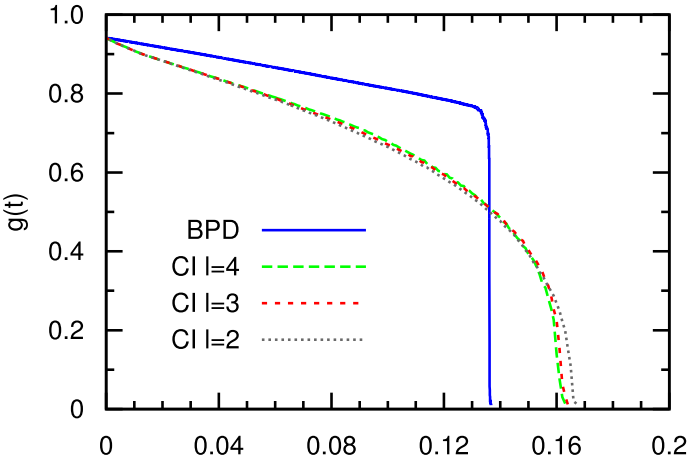
\includegraphics[width=0.7\textwidth]{bpd-ci-comparison}
		\caption[Comparison of Belief Propagation Decimation and Collective Influence]{Comparison of BPD with CI algorithm. On x-axis is the normalized time step and on y-axis is the largest component remaining in the network at time $t$.}
		\label{fig:bpd-ci-comparison}
	\end{figure}
	
	\cite{zdeborova2016} recently extended k-shell decomposition approach with simple fine-tuning. Their algorithm first finds 2-core network and removes the node with highest degree in this network in iterative fashion. This algorithm is named CoreHD, and the results exhibit that it outperforms the CI by a small margin, while significantly reducing the network dismantling time. This method however, focuses more on dismantling and decycling the network faster rather than finding influential nodes. It has not yet been tested under influence spread mechanism.
	
	Overall, BPD is the most efficient; CoreHD has best execution time, while CI is more generic and scalable due to its liberal $l$ parameter.


	\section{Summary}
	\label{sec:related-work-summary}
		
	There are plenty of studies on influence mining and its sub-topics; here is a brief summary of these. The problem of influence maximization, first defined by \cite{kempe2003} was generalized by \cite{leskovec2007b}. A few variations of the same problems were studied by researchers like \cite{goyal2011,morone2015} to view it in dimensions other than conventional network heuristics. The following list summarizes different groups of studies in the domain with prominent works:
	
	\begin{itemize}
		\item On algorithm Optimizations: Great many studies target scalability and efficiency problem on large networks \cite{chen2009,tang2009,chen2010b,goyal2011b,goyal2012,chen2012,jung2012}.
		
		\item Some of the key studies focused on learning influence probabilities for LT, IC and other models, including both classic \cite{granovetter1978} and recent \cite{saito2008,goyal2010}.
		
		\item On identifying Influence: Gladwell thoroughly explained social attributes of influential people in his book \cite{gladwell2006}; \cite{mcpherson2001} define homophily in social networks. On the other hand, Singla et al. prove the existence of correlation phenomenon \cite{singla2008}, while Anagnostopoulos separate influence from homophily and other sources of correlation \cite{anagnostopoulos2008}. On the same idea, \cite{aral2009,lafond2010} later performed randomization tests to distinguish influence from homophily.
		
		\item On Viral Marketing: Studies like \cite{mahajan1990,domingos2001,goldenberg2001,richardson2002,domingos2005,hill2006,leskovec2007,watts2007b,wortman2008,hu2014,barbieri2014} focus on its application in viral marketing, which is clearly a target real-world problem for influence mining \cite{jurvetson2000}.
		
		\item On applications in Social Networks: A cohort of researchers have focused primarily on social networks \cite{borodin2010,ienco2010,bakshy2011,li2013} by examining links between friends and their activities.
		
		\item On Diffusion: the term describing phenomenon of information propagation, has been consistently discussed by many researchers, like \cite{gruhl2004,song2006,song2007,watts2007,anagnostopoulos2008,crandall2008,cha2009,xiang2010,rodriguez2010,rodriguez2011,romero2011,myers2012,li2013,cheng2014,farajtabar2015}.
		
		\item On Veracity: One of the major problems in studying influence in social networks is accuracy of information. \cite{goldenberg2001,guha2004,ziegler2005,golbeck2006,taherian2008,castillo2011,chen2011,holthoefer2012,morone2015,farajtabar2015} attack this critical issue. Lyons showed how serious the information reliability can become in certain applications \cite{lyons2011}.
		
		\item On Context awareness: Some researchers involve context awareness to the problem, rather than core network properties. For example, Haveliwala \cite{haveliwala2002} apply topical detail on PageRank algorithm, while \cite{liu2010,weng2010,li2012} discuss topic-level influence mining. \cite{carnes2007,bakshy2009,bohn2011,barbieri2014} include user content in their studies.
		
		\item On Community detection: A whole different sub-topic of influence mining is community detection. This area is explored by \cite{goyal2008,goyal2009,leskovec2012,mehmood2013,sallaberry2013} and many others.
		
		\item On Resilience: \cite{seidman1983,pagerank1999} build the research foundations. \cite{carmi2007,kitsak2010} scaled the problem on large networks. Studies like \cite{goyal2008,borge2012} talk about resilience purely in context of social networks; Mugisha \cite{mugisha2016} connected resilience with probability learning concept; \cite{zdeborova2016} improved the original k-shell decomposition method; \cite{braunstein2016} showed that Eigenvector centrality outperforms other topological methods on Erdos–Rényi graphs in resilience; \cite{morone2015} proposed a state-of-art ranking method which ranks nodes by computing collective influence of its neighbours.
		
		\item Other heuristics: Since influence maximization is a hard problem, several heuristics have emerged to escape the scalability issue of IM. Starting from classic studies \cite{freeman1979,valente1995}, various heuristics have been presented, for example \cite{kempe2005,kitsak2010,chen2011,aral2011,borgs2014,morone2015,tang2015}.
	\end{itemize}

Recent works in influence maximization focuses mostly on identifying influence, how it propagates in a network in both direct and indirect ways, techniques to maximize influence and learning influence probabilities using past action logs (or transaction logs) of nodes and optimizing existing algorithms for huge networks. In most of the cases, researchers initiate the influence computation from nodes selected randomly, or based on a measure. Such methods are effective in some cases, however they can also lead to problems like selection of nodes from a specific portion of network, more iterations to cover whole network, and choosing less-influential nodes. While there has been high focus on exploiting network properties of nodes for influence maximization, researchers have also attempted to explore content alongside network properties. On one hand, inclusion of content and metadata during analysis boosts the accuracy of the models, but the demerit of such approach is that the models produced are bespoke, they can only work on certain data sets for which they were built.

Albiet all the work reviewed, we have learned that the influence maximization problem is still wide open and its applications growing with time. In the next chapter, we will look at the problem from theoretical perspective in order to affirm that this problem is indeed computationally challenging.

%TODO: add a table to highlight the major challenges in the state of art methods

    
	\chapter{Mathematical Proof}
\label{chp:proof}

It is conspiquous from the literature review that the problem of influence maximization is open despite numerous attempts by the research community to obtain an optimal solution. In this chapter, we observe this problem from theoretical spectacle and provide mathematical formulation and related proofs to establish why this problem is going through constant evolution. In first section, the background is provided; section \ref{sec:proof-np-hard} provides evidence of hardness of the problem; in \ref{sec:proof-greedy-solution} we discuss the greedy-based approximation method, which has laid the foundation of a number of heuristics, followed by proofs of monotonicity and sub-modularity of the influence maximization function; section \ref{sec:proof-time-complexity} sheds light on the time complexity of greedy algorithm and its key weakness of recurrance; finally, section \ref{sec:proof-resilience} provides proof of the hardness of resilience problem.


All notations, and symbols used throughout this chapter are specified in Table \ref{tab:proof-notations}

\begin{table}[]
	\begin{tabular}{|l|l|l|}
		\hline
		\textbf{Name}         & \textbf{Symbol} & \textbf{Description}                                                                                                                                                                           \\ \hline
		Network               & $G$               & An undirected, connected network                                                                                                                                                               \\ \hline
		Nodes (Vertices)      & $V$               & A set of nodes in the network $G$                                                                                                                                                              \\ \hline
		Edges                 & $E$               & A set of edges between $V$ nodes in network $G$                                                                                                                                                \\ \hline
		Tau                   & $\tau$            & A set of time stamps when each edge in $E$ was formed                                                                                                                                          \\ \hline
		Active node           & $u$               & \begin{tabular}[c]{@{}l@{}}An individual node in $G$ which is pre-activated during influence \\ process\end{tabular}                                                                           \\ \hline
		Inactive node         & $v$               & \begin{tabular}[c]{@{}l@{}}An individual node in $G$ which is inactive and may be activated \\ during influence process\end{tabular}                                                           \\ \hline
		Timestep              & $t$               & \begin{tabular}[c]{@{}l@{}}The time in which node $u$ attempts to influence other inactive \\ nodes in $G$\end{tabular}                                                                        \\ \hline
		Influence probability & $p_{u,v}$         & Probability with which node $u$ tries to activate node $v$                                                                                                                                     \\ \hline
		Activation Threshold  & $\theta_v$        & \begin{tabular}[c]{@{}l@{}}The threshold value of inactive node $v$ in LT model. $v$ will \\ activate only if the influence probability $p_{u,v}$ exceeds this \\ threshold value\end{tabular} \\ \hline
		Seed Set              & $S$               & \begin{tabular}[c]{@{}l@{}}Set of pre-activated nodes in $V$ which execute the diffusion \\ process\end{tabular}                                                                               \\ \hline
		Action                & $a$               & \begin{tabular}[c]{@{}l@{}}An action performed by node $u$ which is to be spread in the \\ network through influence propagation\end{tabular}                                                  \\ \hline
		Influence             & $\sigma$          & \begin{tabular}[c]{@{}l@{}}Measure of influence. $\sigma_S$ represents the total influence \\ of a seed set $S$ in $G$ after the diffusion process has completed\end{tabular}                  \\ \hline
		Budget                & $k$               & \begin{tabular}[c]{@{}l@{}}The parameter of influence function which specifies how many \\ influential nodes in $G$ are to be identified as seed set $S$\end{tabular}                          \\ \hline
		Size                  & $N$ or $n$        & The number of nodes in $G$, i.e. $|V|$                                                                                                                                                         \\ \hline
		Candidate set         & $Q$               & \begin{tabular}[c]{@{}l@{}}Represents a finite set of candidates $q$, i.e. $Q={q_1,q_2,q_3,...}$. \\ Each candidate is a potential seed set\end{tabular}                                       \\ \hline
		Candidate             & $q$               & \begin{tabular}[c]{@{}l@{}}Set of $k$ nodes of $G$ which are selected as seed set $S$ in a \\ particular diffusion process\end{tabular}                                                        \\ \hline
		New Seed Set          & $T$               & \begin{tabular}[c]{@{}l@{}}Seed set after completing an iteration and adding newly activated \\ nodes to $S$\end{tabular}                                                                      \\ \hline
		Gain                  & $\delta_S$        & \begin{tabular}[c]{@{}l@{}}Marginal gain, i.e. difference in influence in time step $t+1$ as \\ compared to previous time step $t$\end{tabular}                                                \\ \hline
		Number of simulations & $c$               & \begin{tabular}[c]{@{}l@{}}The number of Monte Carlo iterations to perform to calculate \\ approximate value of influence spread\end{tabular}                                                  \\ \hline
		Inactive set          & $X_S$             & Set of inactive nodes in $G$, i.e. $V-S$                                                                                                                                                       \\ \hline
		Vertex Cover Set      & $V'$              & \begin{tabular}[c]{@{}l@{}}Set of $k$ nodes in $G$ such that all other nodes are directly \\ connected with at least one of the nodes in $V'$\end{tabular}                                     \\ \hline
	\end{tabular}
	\caption[Notations for algorithms and proofs]{Glossary of all notations used in this chapter. All symbols are consistent throughout the document.}
	\label{tab:proof-notations}
\end{table}


	\section{Problem formulation}
	\label{sec:proof-formulation}
	We formulate the influence maximization problem following the footsteps of past studies \cite{domingos2001,kempe2003}. Beginning with an information diffusion model, the input is an undirected, edge-weighted and time-stamped graph $G=(V,E,\tau)$ where $V$ is the set of nodes, $E$ represents set of edges and $\tau$ is a set of time stamps when the links in $E$ were formed. An edge $(u,v)$ represents node $u$ and $v$, connected to each other and their link-formation time is given as $\tau_{u,v}$. An action $a$ is performed by $u$ in time step $t$, which makes $u$ active. Based on certain diffusion model, active nodes in $S$ try to independently influence other inactive nodes in time step $t+1$ in the network either based a probability $p_{u,v}$ by tossing a coin, or by exerting influence collectively on an inactive neighbour. In either case, node $v$ has only one chance to activate, so if the first attempt fails, it will never become active in the process. Newly active nodes join the process to further activate other nodes in second degree neighbourhood; this process continues until time step limit is reached, or no new nodes become active. An inactive node $v$ does not activate in all cases, for example in the LT model, it will become active only if the sum of incoming weights, or number of active neighbours of $v$, exceeds certain threshold $\theta$ between 0 and 1; this model normalizes the weights such that total weight is no greater than 1.
	
	%In time step $t+1$, the node $u$ independently tosses a coin and on successful flip, it attempts to activate an inactive node $v$ with a probability $p_{u,v}$. Each active node $v$ has only one chance to activate its inactive neighbours, so if the attempt fails, it will never make second attempt. Newly active nodes join the process to further activate their neighbours; this process continues until time step limit is reached, or no new nodes become active. An inactive node $v$ does not activate in all cases, for example in the LT model, it will become active only if the sum of incoming weights, or number of active neighbours of $v$, exceeds certain threshold $\theta$ between 0 and 1; this model normalizes the weights such that total weight is no greater than 1.
	
	\begin{center}
		$\theta_v \leq \sum_{u\neq v} p_{u,v} \leq 1$
	\end{center}
	
	Parameter $p_{u,v}$ is chosen at random due to lack of knowledge about the node's tendency to be influenced; we average over possible thresholds for all nodes by randomizing.
	
	There are some key prerequisites to the diffusion phenomenon which are assumed to be true for any diffusion model to apply:
	\begin{enumerate}
		\item Influence is not reflexive function, i.e. a node does not exert influence on itself; an edge $(u,v)$ represents a bond between $u$ and $v$, which was created before action time $t_a$.
		
		\item Once a node becomes active, it never deactivates.
		
		\item A node cannot be influenced if it has no neighbours, thus will not activate.
	\end{enumerate}
	
	The above structure requires a seed set $S$ to compute the influence. Instead of selecting these nodes randomly, some heuristic can also be used, (like node-centrality \cite{freeman1979}) in order to initiate the diffusion process in better condition than random by selecting the nodes in $S$ that are most likely to result in maximum influence spread. Mathematically, in a graph $G(V,E)$, the objective is to extract a subset of nodes $S\subseteq V$ of size $k$ such that it maximizes the influence $\sigma$ in $G$. The goal is to find a set $S|S\subseteq V;|S|=k;k\leq |V|;\sigma_S=max(\sigma_Q)$ where $Q$ is the set of all combinations of $k$ nodes in $V$.
	
	% First prove that this problem has exponential growth
	Let $N=|V|$ be the size of $G$. A candidate set $Q$ denotes a set of all combination sets $q$ of nodes from $V$ of size $k$. Since it is not known which candidate set $q$ in $Q$ has the maximum influence $\sigma$, therefore in order to discover global optimum solution, we need to compute $\sigma$ for all candidates in $Q$.
	
	For $k=1$, $Q=\{q_1,q_2,q_3,...,q_N\}$, i.e. $q_1=\{v_1\}$, $q_2=\{v_2\}$, $q_3=\{v_3\}$, ..., $q_N=\{v_N\}$. Therefore, $|Q|=N$, and the complexity is $O(N)$.
	
	For $k=2$, $Q=\{q_1,q_2,q_3,...,q_N\}$, i.e. \\
	$q_1=\{v_1,v_2\}$, $q_2=\{v_1,v_3\}$, $q_3=\{v_1,v_4\}$, ..., \\
	$q_{N+1}=\{v_2,v_3\}$, $q_{N+2}=\{v_2,v_4\}$, $q_{N+3}=\{v_2,v_5\}$, ..., \\
	$q_{2N+1}=\{v_3,v_4\}$, $q_{2N+2}=\{v_3,v_5\}$, $q_{2N+3}=\{v_3,v_6\}$, ..., \\
	$q_{N*(N-1)}=\{v_{N-1},v_N\}$. Therefore $|Q|={N\choose 2}=\frac{N*(N-1)}{2}$ and the complexity is $O(\frac{N^2}{2})$
	
	The size of the sets can be identified by the combinatorics formula to draw all subsets of size $k$ from $N$, i.e. ${n\choose r}=\frac{n!}{r!(n-r)!}$. In this case, the size of $Q$ for any value $k\leq N$ can be calculated as: $|Q|=\frac{N!}{k!(N-k)!}$. The same can be viewed as $|Q|=\frac{N(N-1)(N-2)(N-3)...(N-k+1)}{k!}$. The time complexity will therefore be $O(N^k+k^{k-1})$, or simply $O(N^k)$. Proving that the computation time is growing exponentially with $k$.
	
	Since we are unable to identify a deterministic polynomial time solution for this problem. The same is also showin in Algorithm \ref{alg:influence-maximization} in which a deterministic exponential time solution is given\footnote{This is a customization of formulation of maximization of sub-modular function \cite{nemhauser1978}}. In next step, we will show that this problem is NP-hard.

	\begin{algorithm}[h]
		\caption{Deterministic exponential time algorithm for Influence Maximization problem}
		\label{alg:influence-maximization}
		\SetAlgoLined
		\KwInput{$G:(V,E);k\leq|V|;\sigma$ (given a connected graph $G$ of $V$ vertices and $E$, budget $k$, and a function $\sigma$ to calculate influence)}
		\KwOutput{$S$ (the set of seed nodes)}
		$Q \gets combinations(V, k)$ (exponential growth)
		\newline
		$S \gets \emptyset$
		\newline
		\For{$q\in Q$}{
			\If{$\sigma_q > \sigma_S$}{
				$S \gets q$
			}
		}
		\Return{$S$}
	\end{algorithm}
	
	% Convert into a Clique problem
	\section{Influence Maximization problem is NP-Hard}
	\label{sec:proof-np-hard}
	The hardness of influence maximization has been discussed by Kempe \cite{kempe2003}, who convert it into Vertex cover problem such that each node in $S$ has an edge with all nodes in $V$. There is a key ingredient missing in their discussion; the vertex cover problem assumes that each node in $G$ is reachable by $S$ directly without discussing influence probabilities, while the node activations are based on certain probability $p_{u,v}$. For $p_{u,v}=0$, the diffusion process will halt without activating any new nodes; for $p_{u,v}=1$, all nodes in the network will activate. In both of these cases, all candidates $Q$ will become equal. Therefore the conditions for influence function will be right only for $0<p_{u,v}<1$. In our proof, we address the special case of approximate value of $\sigma$. In practice we approximate $\sigma$ by performing many trials (Monte Carlo simulations) and average out the results. This is because $\sigma$ is probabilistic and its value can vary in each trial.
	
	Following Cook-Levin theorem \cite{cook1971}, if the Boolean Satisfiability problem (SAT) can be reduced into the the underlying problem in polynomial time, then it will be proven as NP-hard\footnote{NP-complete is an NP-Hard problem for which there exists a non-deterministic polynomial time algorithm}. Instead of direct reduction into the influence maximization problem, we will exploit the transitive property of Cook's theorem:
	
	Let $A$ denote the SAT problem and $C$ denote the influence maximization problem. If we are able to find a problem $B$ such that $A$ can be reduced into $B$ in polynomial time and $B$ can be reduced into $C$ in polynomial time, then $A \alpha C$ will be proven\footnote{The notation $\alpha$ refers to reduction}.
	
	From the graph theory principles, we know that a clique is a fully connected sub-graph of a connected graph, i.e. each vertex in a clique has an edge with every other vertex in that clique.
	
	There are many problems associated with cliques, like Decision problem to check whether a clique of size $k$ exists in a graph $G$ or not, Optimization problem to find the largest possible clique in a graph and Listing problem to find all possible cliques of size $k$ in a graph $G$. The clique decision problem has been proven to be NP-hard \cite{karp1972}. Therefore the listing problem can also be proved as NP-hard, as shown:
	
	Let $B$ be the clique listing problem, i.e. find $L=\{l_1,l_2,l_3,...,l_n\}$; each member $l_i\subseteq V|\forall \{u,v\}\in l_i,\exists E_{u,v}\in E;u\neq v;|l_i|=k$. Meaning $l_i$ is a proper subset of $V$ such that all distinct pairs of vertices $u,v$ have a direct edge $E_{u,v}$ between them. It can be observed that extracting each member in $L$ is a Clique Decision problem, where we check if the member is indeed a clique or not. Hence, the listing problem $B$ is simply $L$ times the Clique Decision problem.
	
	Additionally, we also need to guarantee that the verification function is also P-type. In order to verify that a member $l_i\in L$ is a clique, there must be an edge $(u,v)$ between each pair of nodes in $l_i$. Since the number of edges in each clique is $\frac{k(k-1)}{2}$, the complexity to verify whether the member $l_i$ is a complete graph or not is $O(k^2)$, which is polynomial time.
	
	% Finally, prove that influence maximization problem can be reduced to Clique Listing problem
	Thus far, we have shown that the Clique Listing problem is NP-Hard, i.e. $A \alpha B$. Next we prove that the problem $B \alpha C$ by reducing the Clique listing problem into influence maximization problem.
	
	First similarity between $A$ and $B$ is that the objective parameter for both problems is same, i.e. to find all sets of size $k$. Secondly, both problems can be represented as combinatorial problem, ${N\choose k}=\frac{N(N-1)(N-2)(N-3)...(N-k+1)}{k!}$. Therefore, the candidate sets in $Q$ will be exactly same as the candidate sets in $L$. Therefore the input set of $A$ can be used as input set of $B$. However, the diffusion process is probabilistic rather than deterministic, therefore we run Monte Carlo simulations $c$ times to achieve an approximate value of $\sigma$. The value of $c$ remains constant for all candidates in $Q$. For $A$, the verification problem is a diffusion function $f(A)$ which is run $c$ times, with a complexity of $O(c*(N-k))$ because even if the diffusion process is run exhaustively, each inactive node will be visited only once, therefore the total number of nodes visited will be N-k. On the other hand the verification problem of $B$ is a traversal function $f(B)$ with quadratic complexity of $O(k^2)$. Since $O(N^2) > O(c*(N-k))$, it is proved that problem $B$ can be reduced to $A$ and consequently, $A \alpha C$, i.e. the problem of Influence Maximization is NP-hard.

	Finally, we show that the verification algorithm for influence maximization is non-deterministic, which means that this is not an NP-complete problem. From the algorithm \ref{alg:influence-maximization-verification}, we can see that the function $calculate\_spread(q)$ is probabilisitc and due to randomness in influence attempt, there is no guarantee that $\sigma$ will be same for any $q$ when repeated multiple times. Which is why the verification method cannot be categorized as NP. Therefore, the influence maximization problem is not in class of NP-complete.
	
	\begin{algorithm}[h]
		\caption{Non-deterministic algorithm for optimal solution verification of influence maximization problem}
		\label{alg:influence-maximization-verification}
		\SetAlgoLined
		\KwInput{$G:(V,E),Q={q_1, q_2, q_3, ...},S$ (given a connected graph $G$ of $V$ vertices and $E$, a list $Q$ of candidates of $k$-sizes sets of nodes, a seed set $S$)}
		\KwOutput{the decision whether $S$ is optimal set or not}
		$\sigma_{max} \gets 0$; $q_{max} \gets \emptyset$
		\newline
		\For{$q\in Q$}{
			$\sigma_q \gets calculate\_spread(q)$ (Non-deterministic step)
			\newline
			\If{$\sigma_q > \sigma_{max}$}{
				$\sigma_{max} \gets \sigma_q$; $q_{max} \gets q$
			}
		}
		\If{$q_{max} = S$}{
			\Return{$True$}
		}
		\Return{$False$}
	\end{algorithm}
	

	\section{Greedy solution}
	\label{sec:proof-greedy-solution}
	A common approach scientists take when confronted with an NP-hard problem is to look for a greedy solution which produces results in realistic time, even though the solution may not be optimal. Since the influence maximization problem is NP-Hard, Kempe et. al. \cite{kempe2003} proposed a \textit{Hill climbing} solution based on greedy approach which guarantees approximation within 66\% of the global optimal solution (see section \ref{subsec:related-work-approximation}).
	
		\subsection{Hill climbing algorithm}
		Algorithm \ref{alg:influence-greedy-solution} describes the application of Hill climbing technique on influence maximization problem.
		
		\begin{algorithm}[h]
			\caption{Greedy based Hill climbing solution for Influence Maximization}
			\label{alg:influence-greedy-solution}
			\SetAlgoLined
			\KwInput{$G:(V,E);k\leq|V|;\sigma$ (given a connected graph $G$ of $V$ vertices and $E$, budget $k$, and a function $\sigma$ to calculate influence)}
			\KwOutput{$S$ (the set of seed nodes)}
			$S \gets \emptyset$
			\newline
			\While{$|S|<k$}{
				$\mu \gets \emptyset$
				\newline
				\For{$v\in (V-S)$}{
					\If{$\sigma_{S\cup v}>\sigma_{\mu}$}{
						$\mu \gets v$
					}
				}
				$S \gets S\cup \mu$
			}
			\Return{$S$}
		\end{algorithm}

		\subsection{Approximation guarantee}
		\label{subsec:related-work-approximation}
		Nemhauser's \cite{nemhauser1978} theorem proposed that if a function fulfils Monotone and Sub-modular property, its Greedy approximation will satisfy Eq. \ref{eq:approx-guarantee}. Fortunately, with an added condition that when $S$ is to be grown increasingly, i.e. starting with one node, more nodes are added to the set iteratively, the influence maximization hold these two properties. This allows us to apply Hill climbing solution with high approximation guarantee, i.e.:
		
		\begin{equation}
			\label{eq:approx-guarantee}
			\sigma(S)\geq (1-\frac{1}{e})\sigma_{max}(S)
		\end{equation}
	
		In equation \ref{eq:approx-guarantee}, $S$ is the seed set; $\sigma$ represents the quantity of influence; $\epsilon$ is the exponential constant (its approximate value is 2.718).

		\subsection{Monotonicity property}
		\label{sec:proof-monotone}
		A function is defined to be Monotone if $\forall S\subseteq T, f(S)\leq f(T);f(\emptyset)=0$. Where $T$ is any set of entities in a domain and $S$ is any finite subset of $T$, and $f$ is the underlying function applicable on both $S$ and $T$. Meaning that enlarging the input set does not cause the output to decrease.
		
		The influence maximization function is monotone, i.e. growing the budget $k$ will not cause the influence spread to reduce; it will either increase or remain same.
		
		\textbf{Proof}: For all seed sets $S$, the property $f(S)\leq f(T);f(\emptyset)=0$ is true.
	
		\begin{enumerate}
			\item For $S=\emptyset,f(S)=0$ is true because no nodes will be activated without a seed set.
			
			\item For $k=|V|,f(S)=f(T)$ is true because all nodes are already in the seed set.
			
			\item For $k<|V|$, the candidate nodes $\{V-S\}$ will activate based on activation probability $p=[0,1]$.
			
			\begin{itemize}
				\item For $p=0,f(S)\leq f(T)$ is true because no new nodes will activate in diffusion process, i.e. $f(S)=f(T)$.
				
				\item For $p\leq 1$, the function $f(T)$ will grow by an approximate margin of $p$, i.e. $f(T)\approx f(S)(1+p)$. Therefore $f(S)\leq f(T)$ will hold true.
			\end{itemize}
			
		\end{enumerate}

		\subsection{Sub-modular property}
		\label{sec:proof-submodular}
		A function is sub-modular if $\forall S\subseteq T, f(S\cup \{u\})-f(S)\geq f(T\cup \{u\})-f(T);f(\emptyset)=0$. Meaning that the marginal gain (difference between the gain in previous input set and increased input set) does not increase by enlarging the input set. This property is also know as law of diminishing returns.
		
		The influence maximization function for an increasing set is sub-modular, because as the budget $k$ grows, the growth margin by which the influence is spreading will keep reducing.
		
		\textbf{Proof}: for all seed sets $S$, the property $f(S\cup \{u\})-f(S)\geq f(T\cup \{u\})-f(T)$ is true.
		
		% The proof is basically that the gain of adding 1 node when the seed set is smaller is always equal or larger than the gain of adding 1 node when the seed set is larger, i.e. diminishing returns.
		\begin{enumerate}
			\item For $S=\emptyset,T=\emptyset$ then $f(S\cup \{u\})=f(T\cup \{u\})$ is true as the same node $u$ is the only one active.
			
			\item For $k=|V|,f(S\cup \{u\})=f(T\cup \{u\})$ will be true because there will be no gain when all nodes are already active.
			
			\item For $k<|V|$, let $X_S=\{V-S\}$ be the area of inactive nodes before the diffusion process and $X_T=\{V-T\}$ be the area of inactive nodes after the diffusion process. Also, let the marginal gain $\delta_S$ is the gain of $S$ and marginal gain $\delta_T=$ be $\delta_S$ - $f(T)$. We know from previous proof that during the diffusion process, new nodes activate with probability $p$. Therefore the expected gain of $S$ $\delta_S\approx |X_S|(1+p)$ will be from a larger area of inactive nodes, and expected gain of $T$ will be $\delta_T\approx |X_T|(1+p)-\delta_S$.
			Hence, $\delta_S\geq \delta_T$ will hold true.
		\end{enumerate}
	
	
	\section{Recursive nature and time complexity}
	\label{sec:proof-time-complexity}
	Hill climbing method is recursive in nature, i.e. each step requires input from prior step. Therefore unlike the optimal solution, a solution cannot be driven in parallel execution. On a supercomputer with hundreds of thousands of compute units, it may actually be faster to find an optimal solution on a network than using Greedy algorithm. The time complexity of Hill climbing solution depends upon three main factors, the size of the graph $N$, budget $k$, and the number of simulations $R$. Some researchers also include a fourth factor, i.e. the time it takes to flip the coin \cite{kempe2005}. But in reality, this event can be independently performed before simulations in linear time. The complexity of Hill climbing method is therefore $O(N.k.R)$. Despite the discussions and state-of-art being furthered each day by the research community, Hill Climbing is still the top heuristic which guarantees an approximate solution closest to the optimal solution in terms of accuracy; this is due to its tendency to evaluate the whole network from scratch in each iteration\footnote{The experiments in chapter \ref{chp:inf-framework} also show this to be true.}. It can therefore be considered for all small scale networks where quadratic time complexity is tolerable in terms of number of nodes.
	
	
	\section{Network dismantling problem is NP-Complete}
	\label{sec:proof-resilience}
	We discussed that the resilience problem is connected with influence maximization in previous chapter. Here we show that the network dismantling problem (which is closely related to resilience) is also NP-complete, and while the problem of finding the optimal set of influential nodes can also be solved by transforming it into resilience problem (as experimentally shown in chapter \ref{chp:inf-framework}), this approach does not reduce the complexity of original problem.
	
	Following the lead \cite{braunstein2016}, we start with a fully connected graph, i.e. Clique and reduce it to Vertex Cover decision problem\footnote{Note that the minimum vertex cover problem is NP-hard.}, i.e. to find if a set of size $k$ exists such that every other node in the graph is reachable within one hop distance by this $k$-set. Mathematically:
	% Find a subset of nodes such that for each edge i,j, either i is in that subset or j in that subset
	For graph $G=(V,E)$, find a subset $V'\subset V|\forall (i,j)\in E, i\in V' \vee j\in V'$.
	
	We introduce a constant $k$ to denote the size of the required vertex set. Therefore the problem becomes identifying $V'$ such that $|V'|=k$.
	
	The best case scenario for this problem is a Clique, in which for all values of $k$, the node set will solve the vertex cover problem in $O(1)$ as all nodes are fully interconnected. However, the complexity exponentially worsens on random and complex networks, just as in the case of influence maximization.
	For $k=1$, the universe of possible sets is $V'=\{u_1\},\{u_2\},\{u_3\},...,\{u_n\}$, i.e. $O(n)$.
	For $k=2$, the universe of possible sets is $V'=\{u_1,u_2\}$, $\{u_1,u_3\}, \{u_1,u_n\}, ..., \{u_2,u_3\}, \{u_2,u_4\}, \{u_2,u_n\}, ..., \{u_{n-1},u_n\}$, i.e. $O(n^2)$.
	Therefore, for $k=3$, the complexity will be $O(n^3)$. Naturally, the complexity of the problem is $O(n^k)$.
	
	The time complexity of Vertex cover problem for worst case scenario requires computation of all combinations of size $k$, therefore the complexity will be $O(n^{\frac{k(k-1)}{2}})$. Thus the problem is not P-type. We can present an NP solution where the non-deterministic part is a function to identify the $V'$ as shown in algorithm \ref{alg:min-vertex-cover}. The algorithm starts computation of all combinations of nodes of size $k$, i.e. $Q$; finally for each candidate $q\in Q$ it checks whether $q$ solves vertex cover problem. The process exits as soon as a set which covers the graph vertex is identified.
	
	\begin{algorithm}[h]
		\caption{Non-deterministic Polynomial time algorithm for minimum vertex cover problem}
		\label{alg:min-vertex-cover}
		\SetAlgoLined
		\KwInput{$G:(V,E);k$ (given a connected graph $G$ of $V$ vertices and $E$; some constant $k<|V|$)}
		\KwOutput{$V'$ (the set of nodes covering vertex)}
		$V'\gets \emptyset$; $Q\gets combinations(V, k)$ (exponential growth)
		\newline
		\For{$q\in Q$}{
			\If{$\forall (i,j)\in E, i\in q \vee j\in q$}{
				$V'\gets q$; \textit{break}
			}
		}
		\Return{$V'$}
	\end{algorithm}

	We now show that the problem of finding a set of $k$-nodes which dismantles the network can be reduced to vertex cover decision problem. Let the network dismantling problem be $A$ and vertex cover problem be $B$. The objective of $B$ is aforementioned; the objective of $A$ is to idenfiy $S\subset V;|S|=k$ in $G$ such that when $S$ is removed, the network $G$ is maximally dismantled, i.e. no other set of size $|k|$ reduces $G$ on removing it from the network as much as $S$ does.
	
	%The result of this activity is a set of many connected subgraphs $G'\subset G$; we identify the largest of these connected subgraphs and repeat the same algorithm.
	The process repeats until the network is completely dismantled, i.e. there are no conneced nodes remaining in the largest component.
	
	We can reduce the problem of network dismantling into vertex cover problem. First, an instance of $A$ is also an instance of $B$, i.e. the set identified by $S=f(A)$ is exactly same as the set identified by $V'=f(B)$ for same graph $G$ (where $f$ represents objective function of each problem). Secondly, where $B$ verifies whether the set $V'$ has an edge with each other node in $G$ or not, the problem $A$ removes the nodes in $S$ and checks if the graph is dismantled. For $A$ if the graph is not completely dismantled then we say that no set of size $k$ exists to sovle dismantline problem; for $B$ if all nodes in $V$ are not connected with $V'$, then we say that no set of size $k$ exists to solve the vertex cover problem. The time complexity of finding the set in both cases is exactly same, i.e. $O(n^{\frac{k(k-1)}{2}})$.
	
	Similarly, the verification problem of $A$ can also be reduced in polynomial time. For $B$, we can verify that all nodes have an edge with at least one of the nodes in $V'$ in time $O(|E|*k)$. For problem $A$, we can verify that there does not exist an edge between any pair of nodes in $O(|E|)$. Both are P-type, hence the dismantling problem can be reduced into vertex cover decision problem, and is therefore NP-complete.
	
	Because of the complexity of network dismantling problem, similar greedy based method is used by iteratively running the dismangling function, removing one or more similar nodes in each iteration. The resilience test is the verification function of network dismantling problem, which returns the largest connected component remaining after removing nodes in $S$ from $G$.
	
	Here, a question rises that why is influence test required when resilience test already exists being an NP-complete problem? The answer lies in the selection of the largest connected component on each iteration, and leaving out the other big components. Figure \ref{fig:resilience-process} is a pictorial representation of this shortness. In the image on left, the network $G$ is shown with node $J$ highlighted as the one with highest degree; the image on the right shows that on removing $J$, the largest connected component has 9 nodes. However, the second largest component with 8 nodes was left out even though it's only one node shorter than the first component. This causes a bias towards the largest component because the second largest connected component is in no manner less significant or less resilient than the first component. The influence test does not inherit such weakness, and thus provides a better alternative especially for sparse networks. \\
	
	\begin{figure}[h]
		\centering
		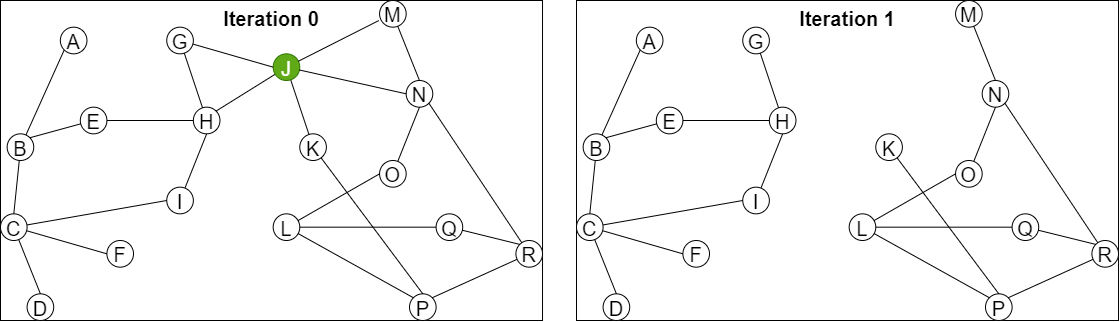
\includegraphics[width=0.9\textwidth]{resilience-process}
		\caption[Network dismantling process]{Network dismantling process. Iteration 1 shows the graph after removing the node with highest degree from original network, thus splitting the graph into two connected components of 9 nodes (left) and 8 nodes (right).}
		\label{fig:resilience-process}
	\end{figure}

This chapter theoretically showed that the influence maximization problem is indeed computationally challenging, which is why this is still an open problem. Next chapter evaluates the same on practical grounds by performing various experiments on a broad range of networks. It is important to note that the proofs presented in this chapter are excerpts from past literature. The notations have been made consistent, the order maintained for completeness, and thorough detail added where needed for reader's convenience.


	\chapter{Study design and experiments}
\label{chp:inf-max}

In this chapter, we present the design of the study and the experiments performed to further the research in the domain of influence mining. Recall from chapter \ref{chp:related-work} where we showed that the problem of identifying most influential nodes in a graph is a global optimization problem. The objective is to find a set $S$ such that there is no other set which maximizes the influence more than $S$. It also proved that this is a difficult problem to solve optimally in real world scenarios. There have been numerous attempts to solve this problem, which has been covered in chapter \ref{chp:related-work} with mixed results but a generalized solution -- one which works for all use cases of influence mining problems -- is still awaited. We attempt to perform various experiments to discover and propose a realistic solution to the influence mining problem.

	\section{Study design}
	Figure \ref{fig:study-design} sums up the study from inception of the problem to proposed solution. Each block in the diagram is expanded into a section of this chapter, starting from data collection to the solution framework.

	\begin{figure}[H]
		\centering
		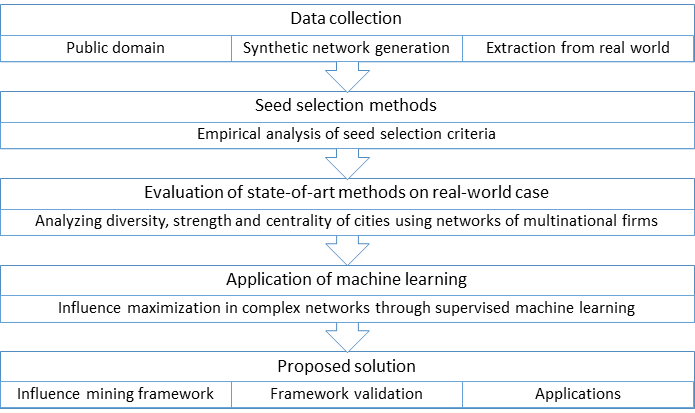
\includegraphics[width=1\textwidth]{study-design}
		\caption[Experiment design]{Study design representing flow of the study from inception to conclusion.}
		\label{fig:study-design}
	\end{figure}
	
		\subsection{Data collection}
		Experiments discussed in this chapter use various network data sets which are obtained from different domains. There are three main sources of the data:
		
		\begin{enumerate}
			\item Public domain: these data sets are collected from public sources. The rationale behind using these data sets is that they appear frequently in past as well as state-of-art researches. In addition, these are in clean, pre-processed form with structural properties already known.
			
			\item Synthetic: such networks are generated via network generator tools. As explained in \ref{sec:domain-synthetic-nets}, they imitate behaviour of real networks but do not contain real-world bias as well as come in handy for bootstrapping purpose when there is scarcity of real-world data.
						
			\item Extracted: some of the networks used have been collected by the author or associates directly from real-world implementations. The primary purpose of these networks is to test methodologies on actual use cases which contain real-world noise and biases.			
		\end{enumerate}
	
		\subsection{Seed selection methods}
		We performed a number of experiments with real world and synthetic networks. The objective of these experiments was to test several seed selection methods used in the literature and analyze whether influence depends only on the structure of a network, or do seed selection methods play a role in spreading influence in different types of networks.
		
		\subsection{Evaluation of state-of-art methods on real-world case}
		Learning from previous experiment, it was established that the seed selection criteria can vary in performance if the structure of network is different. On the other hand, a variety of methods were proposed by the research community, each claiming to outperform existing methods. This experiment was conducted to test CI, a state-of-art seed selection algorithm against known popular methods. The study compares findings with ground truth on multiple dimensions including diversity, strength and centrality of nodes.

		\subsection{Application of machine learning}
		Failing to identify a single heuristic to extract influential nodes in all kinds of networks, we modeled the problem as a supervised machine learning problem, which is a data mining technique. The object was to combine the strengths of multiple seed selection methods and classify influential nodes on various networks to construct a general purpose influence mining model. We started from generating a dataset, consisting of macro and micro level details as features and target labels (influential/non-influential) identified through optimal and greedy algorithms. In the second phase, we trained multiple models, and selected the most accurate model to further test on real-world networks. The study concludes that machine learning is a viable solution to the influence maximization problem for a broad variety of networks with varying structural properties.

		\subsection{Proposed solution}
		Combining the feedback from all experiments performed, it was evident that not only there is an absence of one algorithm which can satisfactorily solve the influence mining problem, but also that existing research focuses only on a single convergence criteria when choosing an influence mining algorithm. Moreover, the algorithms themselves are tested by quantifying the diffusion alone. We argue that both of these fixed settings do not fully address the real-world problems and propose a framework in response which addresses these key observations.


	%%%%%%%%%%%%%%%%%%%%%%
	%%% Experiment - 1 %%%
	%%%%%%%%%%%%%%%%%%%%%%
	\section{Empirical analysis of seed selection criterion}
	\label{sec:inf-max-seed-selection-analysis}
	The foundations of the contribution in this experiment were laid by Hashmi et. al. \cite{hashmi2012} who targeted five semantically different social networks as described in Table \ref{tab:inf-max-social-networks}. These networks were randomly sampled ten times and their statistics were averaged; then these networks were compared using three levels: elemental, group-level and network-level\footnote{These terms are synonymous to the levels discussed in \ref{chp:domain}, i.e. Elementary is Micro-level, Group is Meso-level; Network is Macro-level}. Their results found the networks under observation to be structurally similar with a few exceptions.
	
	\begin{table}[h]
		\centering
		\begin{tabular}{|l|l|l|l|l|l|l|l|}
			\hline
			& \textbf{Edges} & \textbf{Density} & \textbf{HD} & \textbf{Diameter} & \textbf{CC} & \textbf{APL} & \textbf{$\alpha$} \\ \hline
			\textbf{Twitter}   & 3099  & 6.18  & 237 & 11 & 0.19 & 2.6  & 1.57 \\ \hline
			\textbf{Epinions}  & 13739 & 27.47 & 278 & 7  & 0.43 & 1.93 & 1.2  \\ \hline
			\textbf{Wikipedia} & 11672 & 23.34 & 281 & 12 & 0.35 & 2.1  & 1.21 \\ \hline
			\textbf{Email}     & 2396  & 4.79  & 499 & 7  & 0.54 & 1.98 & 1.87 \\ \hline
			\textbf{Co-Author} & 2404  & 4.8   & 102 & 10 & 0.6  & 2.87 & 1.66 \\ \hline
		\end{tabular}
		\caption[Networks statistics of social network data sets]{Networks statistics of social network data sets used. The networks are sampled with size 500 each. HD is highest degree, CC is graph clustering coefficient, APL is average path length and $\alpha$ is the power-law coefficient}
		\label{tab:inf-max-social-networks}
	\end{table}
	
	While the overall results stayed as expected, i.e. the networks exhibited similar structural properties despite being contextually different. However, the authors observed a few exceptions, as shown in Figure \ref{fig:structural-similarity}. The variation in Clustering coefficient and Strength of triads show some structural dissimilarities. For example, in case of email network, the CC is spread across the network rather than lying in core of the network as others. The linear decay in degree distribution for Epinions and Wikipedia networks indicated non-scale free behaviour. And final dissimilarity flagged was that the Closeness centrality significantly varied for email network, suggesting that the very high value of HD caused the drop in closeness for other nodes.
	
	\begin{figure}[H]
		\centering
		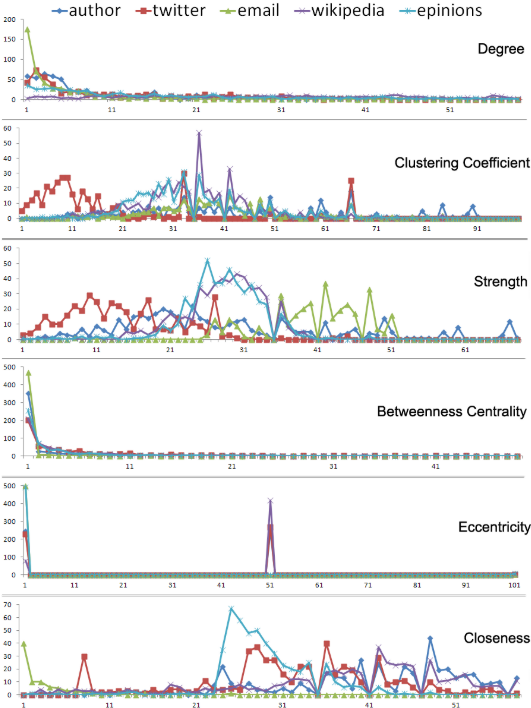
\includegraphics[width=0.7\textwidth]{structural-similarity}
		\caption[Frequency distribution of seed selection metrics of five networks]{Frequency distribution of network metrics. Horizontal axes shows bins of metric values and vertical axes represent frequency of node occurrences \cite{hashmi2012}.}
		\label{fig:structural-similarity}
	\end{figure}
	
	Following the lead from this study, we conduct an empirical experiment \cite{hussain2013a} to closely observe the impact of various seed selection methods on both IC and LT diffusion models on both real and synthetic networks. For diversification, four classes of networks were selected: scale free, small-world, scale free and small-world and random.
	
	%Starting with an undirected graph $G=(V,E)$, each edge $E=(u, v)$ represents that nodes $u$ and $v$ have a direct edge with each other. For IC model, we use chance probability (0.5) to exert influence from active nodes on their inactive neighbours. An inactive neighbour is influenced only once with this probability; consequently, it will either activate and further spread action $a$ or stay inactive. Either way, a node will not be tried for activation twice. In the LT model, each inactive node looks for active nodes in its neighbourhood and if the incoming influence from neighbourhood is above certain activation threshold, the inactive node will also become active.
	
	In given Algorithm \ref{alg:seed-selection}, $G=(V,E)$ is the prerequisite network, $k$ is some budget, $M$ is any function to calculate centrality of nodes ($M_v$ represents centrality of a single node; $M_{V}$ means centrality of all nodes in $V$) and $\sigma$ is a function to calculate the spread or influence of selected seed set. Note that instead of learning influence probabilities, we used chance probability (0.5).
	
	\begin{algorithm}[h]
		\caption{Diffusion algorithm using various seed selection methods}
		\label{alg:seed-selection}
		\SetAlgoLined
		\KwInput{$G:(V,E);k\leq|V|;M;\sigma$ (given a connected graph $G$ of $V$ vertices and $E$, budget $k$, a function $M$ to compute node centrality; influence quantifier $\sigma$)}
		\KwOutput{$\sigma$ (the number of nodes influenced successfully)}
		$S \leftarrow \emptyset$; $\sigma \leftarrow 0$
		\newline
		\While{$|S|<k$}{
			$S \leftarrow S \cup (v|M_{v}=max(\{M_{s}\})$ (pick the node $v$ with maximum centrality value in remaining nodes)
		}
		$W \gets V-S$
		\newline
		\While{$W \neq \emptyset$}{
			$A \leftarrow \emptyset$
			\newline
			\For{$v \in W$}{
				$N \leftarrow u|u \in S; (u,v)=1$; $\theta \leftarrow rand(0,|N|)$
				$sum \leftarrow \Sigma_{i=1 to |u|} j=rand(0,1)$ (toss a coin for each neighbour and sum up the number of successes)
				\newline
				\If{$sum \geq \theta$}{
					$A \leftarrow A \cup {v}$
				}
				$W \gets W-{v}$
			}
			$S \leftarrow S \cup A$; $\sigma \leftarrow \sigma + |A|$
		}
		\Return{$S,\sigma$}
	\end{algorithm}

	First phase of the algorithm executes a loop. In each iteration, a node with highest centrality score is picked and added to seed set $S$. The next phase runs iteratively until no nodes are left which have not been attempted for activation. The nodes activated successfully by $S$ are removed from graph iteratively; each node $u$ attempts to activate inactive nodes in $v\in V$ by chosing a random threshold. If the total sum of active nodes in $S$ who have successfully attempted to activate $v$ exceeds this threshold $\theta$ then $v$ is activated and added to the set $S$ for next iteration. When the loop ends, all $v$ nodes which have been attempted are removed as they will never be activated again. The influence is then recalculated based on newly activated nodes in $S$. At the end, total influence $\sigma(S)$.
	
		\subsection{Experiment settings} 
		The experiment performed for empirical analysis of seed selection methods uses both real and synthetic networks. The networks generated were small world (SW) using the model from \cite{watts1998}, scale free (SF) using the model from \cite{barabasi1999}, small world-scale free network (HK) using the model of \cite{holme2002} and random network (RD) using the model network of \cite{erdos1960} to represent different types of networks. Small world model can be generated for the desired number of nodes and edges by starting with a regular graph in which each node has a degree $n$. In scale free model nodes are attached preferentially therefore for every new node we can tune the number of edges to make a scale free network. Small world-scale free model can also be tuned by the number of nodes to which each new node connects to, which will give us the desired edge-node ratio. We have generated a random network with $n$ nodes and $m$ edges whose degree distribution $p_k$ follows the Poisson distribution $p_k = e^{-\lambda} \frac{\lambda^k}{k!}$ . In our generated networks , all had $\lambda > 1$ which indicates that most nodes have the degree close to the mean degree of the network.
		
		The real networks include Political Blog, Twitter, Epinions and Author networks which are briefly described below:
		
		\begin{enumerate}
			\item Political Blog: hyperlinks network between weblogs on US politics, which was recorded in 2005 by Adamic and Glance \cite{adamic2005}. Each node represents a blog post while an edges are links between blogs, which were automatically detecting by crawling the links on front page of blogs.
			
			\item Twitter: famous micro-blogging social network. The data set used is originally extracted by \cite{hashmi2012}. A node is a registered user account, while an edge between two nodes means any one or both users have followed the other.
			
			\item Epinions\footnote{\url{http://snap.stanford.edu/data}}: a who-trust-whom online network at Epinions.com, a customer analysis website. To trust each other, site members can either agree or disagree. Trust is formed by the interaction of all the reliable contacts which is on the basis of review ratings.
			
			\item Author\footnote{\url{http://vlado.fmf.uni-lj.si/pub/networks/data/}}: a co-authorship network, generated from the BibTeX bibliography developed from the Computational Geometry Database. Each author is a node and two authors form an edge if they have contributed to same work together, e.g. an article, book etc.
		\end{enumerate}
		
		The real data sets were reduced to the largest connected components. Then, the synthetic networks were generated equivalent to the real networks in structure, i.e. five simulated networks for each class equivalent to the four real social networks, summing up to a total of 80 networks. The rationale behind selecting multiple data sets for experimentation is to ensure accuracy, since the information diffusion in each model is based on random choices (see Table \ref{tab:inf-max-social-networks-2}). An important similarity among all these networks is the low average path length and high clustering coefficients of these networks giving them small world properties except random networks. Scale free networks have low clustering coefficient and the degree distribution of small world and random networks follows a Poisson distribution with $\lambda >1$. As an example, Table \ref{tab:inf-max-empirical-analysis-apl} explains how the APL of these networks compare.
		
		\begin{table}[h]
			\centering
			\begin{tabular}{|l|l|l|l|}
				\hline
				& \textbf{Nodes} & \textbf{Edges} & \textbf{Density} \\ \hline
				\textbf{Blog}     & 1222           & 16714          & 13.6             \\ \hline
				\textbf{Twitter}  & 2492           & 17658          & 7                \\ \hline
				\textbf{Epinions} & 2000           & 48720          & 24.3             \\ \hline
				\textbf{Author}   & 3621           & 9461           & 2.6              \\ \hline
			\end{tabular}
			\caption{Size, number of edges and density of the four real networks used.}
			\label{tab:inf-max-social-networks-2}
		\end{table}
		
		\begin{table}[h]
			\centering
			\begin{tabular}{|l|l|l|l|l|l|}
				\hline
				\textbf{Data set} & \textbf{Real} & \textbf{RD} & \textbf{SW} & \textbf{SF} & \textbf{HK} \\ \hline
				\textbf{Blog}     & 2.7           & 2.5         & 3.2         & 2.4         & 2.2         \\ \hline
				\textbf{Twitter}  & 3.4           & 3.2         & 4.2         & 2.9         & 2.8         \\ \hline
				\textbf{Epinions} & 2.2           & 2.2         & 3           & 2.2         & 2           \\ \hline
				\textbf{Author}   & 5.31          & 5.07        & 6.41        & 3.4         & 4           \\ \hline
			\end{tabular}
			\caption{RD, SW, SF, HK mean that synthetic network was extracted using a synthetic network generator using: Random model, Small-world model, Scale Free model, and Holme and Kim Model (small world-scale free networks) respectively. The value represents average APL for each class in all real and generated networks.}
			\label{tab:inf-max-empirical-analysis-apl}
		\end{table}
		
		\subsection{Results}
		Figure \ref{fig:empirical-analysis-influence} describes the influence spread as well as the iterations it took for each method to reach all nodes. There are some key findings from this experiment, as evident from results:
		
		\begin{itemize}
			\item The first observation from the results of influence spread is that the behavior of small world networks and random networks is the same for all the different seed selection strategies with a lone exception of closeness centrality on Twitter. The reasons here is an important similarity in small world networks and random networks; their APL is low, but since both of these two classes of complex networks are missing very high-degree nodes, the algorithms behaves similarly for all the different seed selection methods.
			
			\item Small world networks have high clustering coefficient due to abundance of triads. On the other hand, random networks have scarcity of triads. It is therefore expected for small-world networks to exhibit high influence spread, but to our surprise, no significant impact of clustering coefficient was evident during our experiments; rather, high-degree nodes contributed more in the influence spread.
			
			\item In real networks, scale free networks (SF) and small world-scale free networks (HK), the betweenness centrality leads the other metrics in spreading maximum influence followed closely by degree centrality.
			
			\item Closeness performs well for the Twitter network whereas for the other three data sets, the closeness and random selection have only minor differences.
			
			\item Eigen-vector performs well for small world-scale free and scale free networks, even better than betweenness centrality for the Epinions network. Interestingly, the Eigen-vector centrality is quite variable in performance on real networks. It performs poorly for Twitter network, worse than closeness. It performs very close to betweenness and degree centrality for Epinions and has a notable difference for Blog and Author networks.
			
			\item The similarity between real networks and HK are notably high. This reaffirms that most real world networks are both small world and scale free in nature. An exception to this narrative is Author data set, but it can be argued that this is due to the marginal difference in high degree. Original network has high degree 102, while its SF and HK counterparts have 201 and 183 respectively.
			
			\item In terms of iterations, betweenness centrality performs well along with degree and eigen-vector centrality except for the case of small world and random networks generated equivalent to the Author network. An exception again, is Author network which required more iterations. However, this time it is due to the density of the network as well as relatively low value of high-degree node. Epinions networks also proves the above conjecture, as the highest degree node in the real Epinions network is with degree 1192, which is more than 50\% of the nodes are connected to a single node.
			
			\item The edge density and the number of iterations show signs of negative correlation; the most dense network (24.3) of Epinions took an average of 2.4 iterations; Political Blog network with density of 13.6 averaged 3.0 iterations; Twitter with a density of 7 finished iterating with an average 3.6; the Author network of density only 2.6 took most average iterations of 4.8. Concisely, the denser a network is, the less iterations it takes for influence process to complete.
			% The above point was indicated by Dr. Guy Melancon in his review feedback
			
			\item Lastly and as expected, the APL exhibited uniform behaviour in almost all the experiments. The number of iterations on all of the Epinions and Blog data sets, having low APL remained between 2 and 5. Twitter data set took 6 iterations for RD in random influence method and 5 iterations for the rest of the methods. However, on Author data set with highest APL, the number of iterations begin from 4 and hike to 8. This is because it requires less number of steps to traverse from one node to another in the network.
		\end{itemize}
		
		\begin{figure}[H]
			\centering
			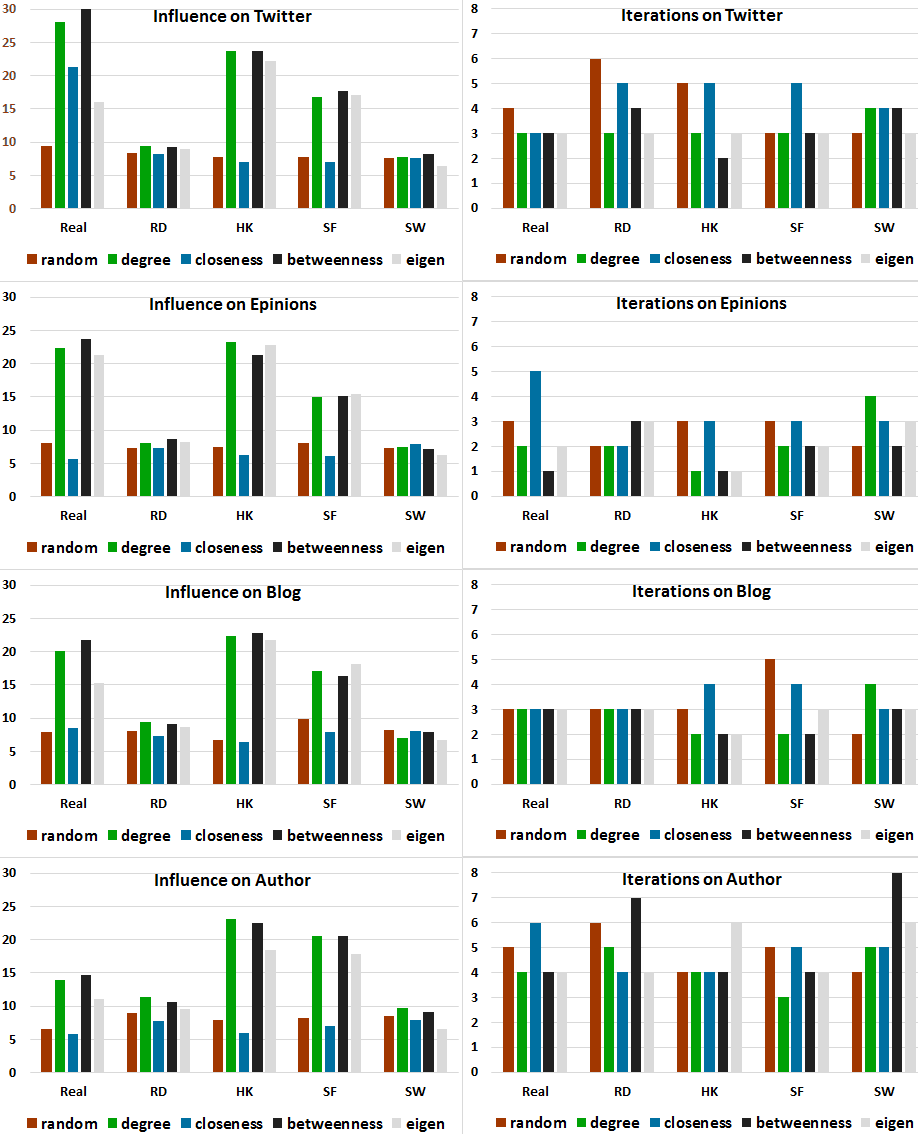
\includegraphics[width=0.8\textwidth]{empirical-analysis-influence}
			\caption[Influence spread and number of iterations on networks]{Figure showing bar graphs for the data sets and their simulated networks. Bars on the left side represent the average percentage of total nodes influenced during diffusion process with budget $k=5\%$. Bars on the rights side represent the average number of iterations that the algorithm took to try to spread the influence to whole network. The results are aggregate of all 80 networks generated.}
			\label{fig:empirical-analysis-influence}
		\end{figure}
		
	The key finding from the above experiment is that the seed selection criteria plays less important role than the structure of the network itself in the influence maximization process. Thus solidifying the conjecture that a certain seed selection method can vary in performance on different types of networks.
	
	In the next section, we scrutinize influence mining phenomenon from an application perspective on a real-world case. The aim is not only to see if a state-of-art method outperforms classic heuristics, but also to analyze whether the conclusions drawn from influence maximization method actually match with the ground truth.

%	\newpage

	%%%%%%%%%%%%%%%%%%%%%%
	%%% Experiment - 2 %%%
	%%%%%%%%%%%%%%%%%%%%%%
	\section{Analyzing Diversity, Strength and Centrality of Cities using Networks of Multinational Firms}
	\label{sec:resilience-city-networks}
	In this experiment, we put the resilience methods to test in a real world scenario \cite{hussain2019}. The main objective is to test whether resilience methods are able to successfully identify critical cities in global economic networks. Once the methods were able to identify the critical cities, we studied the economic networks over two time periods 2010 and 2013 to analyze the change in the importance of cities over the two time periods. Secondarily, we observe different influence mining methods and see which of them is more appropriate for further analysis. We analyze diversity, strength and centrality of the cities considering these as key indicators in observing how cities have changed their roles in the global economic networks over time.
	
	In particular, we are looking for the aftermath of great recession that occurred in 2008. Unsurprisingly, this is a very well established field of research and there have been numerous studies focusing specifically on city importance under the lens of economic ties \cite{blumenfeld2009,storper1997,scott2003}. The application of network analysis is also not novel in this area, \cite{barabasi1999,ducruet2014,liu2014} have observed the cities as complex networks before, and have confirmed that the economic ties between cities cause a ripple effect between strongly linked cities when one city is affected both positively and negatively. In particular, \cite{derudder2003,liu2014} explored the hierarchical organization of cities; \cite{taylor2002,taylor2013,alderson2004} focus on topological view of these cities; \cite{sassen2007,sassen2011} study city networks from the perspective of spatial concentrations forming economic hubs; closely tied to the financial hubs, \cite{ducruet2011,beaverstock2002} explore the densely connected components, often referred to as communities in SNA, especially \cite{liu2014} applied hierarchical community detection to find hierarchical and temporal patterns.
	
	The application of resilience problem on city networks although is not new in this arena, it is rare to some degree. Barthélemy \cite{barthelemy2011} and Okelly \cite{okelly2014} have previously explored the resilient cities in search of identifying most dominant economies. In this regard the rise of China as a global economic power, as well as the Gulf region is widely studied and accepted \cite{alderson2010,mahutga2010,derudder2010}. Our findings re-assert this rise between 2010-2013; however the main objective is to identify other cities and global regions which exhibit similar significance but are either non-trivial to find, or are overlooked.
	
		\subsection{Data set}
		The underlying experiment uses a data set consisting of two networks from year 2010 and 2013 of economic ties of multinational firms and their subsidiaries. Each node represents a city\footnote{The term city is used loosely here, they actually represent a large urban area delineated with the a standard criteria (see \cite{rozenblat2017}). For example, Paris represents all the smaller towns and cities located around it.} where an edge is an ownership connection between two organizations located in the cities, i.e. if two cities have an economic and financial link and belong to the same group of companies, an edge is formed. The world's leading 3000 multinational groups of companies with 800,000 direct and indirect subsidiaries are used to build the network, forming 1 million edges between them. The top group of companies were selected based on their annual turnover and made available by Bureau van Dijk\footnote{Bureau van Dijk Electronic Publishing (\url{http://www.bvdep.com/)}}.
		The data has been extensively processed to clean incorrect fields and complete missing values at the Universit\'{e} de Lausanne - ERC GeoDiversity research group\footnote{ORBIS 2010, 2013: BvD - Universit\'{e} de Lausanne, ERC - Geodiversity, Switzerland)}. These networks are similar in construction but larger in size to other datasets \cite{kraetke2014,wall2011,alderson2004} extensively used to represent economic networks of cities. Figure \ref{fig:city-network-construction} depicts the construction of these networks. Table \ref{tab:resilience-city-network-stats} shows a quantitative summary of different measures for the two networks constructed, one for the year 2010, and the other for 2013.
		
		\begin{figure}[H]
			\centering
			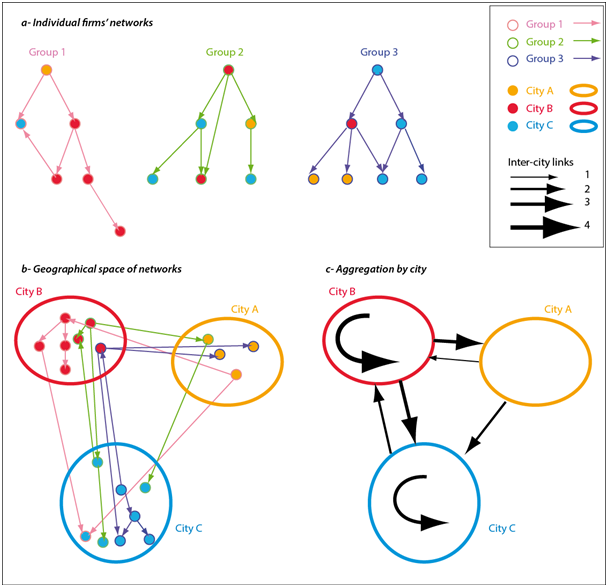
\includegraphics[width=0.8\textwidth]{city-network-construction}
			\caption[Hierarchy of economic network of multinational firms]{Construction of Economic Networks of Cities: (a) Hierarchy of Multinational Firms and the links to their Subsidiaries (b) Firms are Geographically Distributed and (c) Links are aggregated to connect cities forming Economic Networks. \cite{rozenblat2017}}
			\label{fig:city-network-construction}
		\end{figure}
	
		The networks have high similarity in highest degree and transitivity measures. While transitivity tells how many triads of cities are there, highest node degree explains the maximum number of unique connections a city has with others.
		
		A key observation from 2010 to 2013 is that the number of new nodes and connections have grown, which is a hint on how the multinational firms are opting their strategy of expansion. This could be caused due to two main reasons: either the firms have opened new franchises or acquired new partners to increase their footprint, or they have risen to the top 3000 multinational companies in 2013, and are therefore reflected in new network
		
		\begin{table}[h]
			\centering
			\begin{tabular}{|l|l|l|}
				\hline
				\textbf{Metric}                     & \textbf{2010} & \textbf{2013} \\ \hline
				Cities (Represented by Nodes)       & 1206          & 1253          \\ \hline
				City-City Linkage (Unweighed Edges) & 28639         & 31704         \\ \hline
				Node-Edge Ratio                     & 23.7          & 25.3          \\ \hline
				Highest Degree                      & 762           & 777           \\ \hline
				Average Path Length                 & 2.29          & 2.27          \\ \hline
				Transitivity                        & 0.331         & 0.339         \\ \hline
			\end{tabular}
			\caption[Quantitative comparison of the both instances of city networks]{Network Statistics: Quantitatively comparing the two networks. Different network metrics show the structural similarity of the two networks.}
			\label{tab:resilience-city-network-stats}
		\end{table}
	
		\subsection{Experiment settings}
			
			\subsubsection{Diversity, Strength and Centrality}
			To define the importance of a city, three notions are used, namely \textit{Diversity}, \textit{Strength} and \textit{Centrality}:
			
			\begin{enumerate}
				\item Diversity: we describe Diversity as a measure of importance of a city based on the number of connections it has to other unique cities\footnote{In SNA, Diversity can be calculated using Unweighted Degree Centrality}. For example, in figure \ref{fig:city-network-construction} $A$ has three connections with $B$, and single connection with $C$, in terms of diversity. We would therefore say that the diversity of $A$ is 2.
				
				\item Strength: Strength\footnote{Weighted Degree is used to calculate Strength} reflects the total number of connections a city has in the network. Continuing with our example, city $A$ would have a strength of 4 as it has a total of 4 connections, 3 with city $B$ and 1 with city $C$. The higher the number of ties it has with other cities, the stronger it is in the network.
				
				\item Centrality: Centrality is arguably the most widely used metric in network analysis. We used two approaches to compute centrality, first from Global Production and Value Networks \cite{henderson2002,gereffi2005}, which are common in spatial economics, and the other from network connectivity \cite{brandes2005} which is more generic.
			\end{enumerate}
		
			The cities which connect global network are considered pivotal. This in turn can be represented by cities which hold the network together as a single connected network. We estimate this by using the network dismantling method discussed in \ref{sec:domain-resilience}. This connectivity is critical in avoiding economic silos which hinder global trade and economic development thus putting cities with this characteristic in a central position.
		
			Learning from the classical and state-of-art literature, it is clear that no single metric has been proven to be most effective in finding central nodes in different network topology. Since centrality varies based on the topology and structure of a network \cite{hashmi2012,hussain2013a,malighetti2019}, we applied several metrics extensively used in the literature to find the optimal metric for each of the two city networks used in this study.
		
			We used Degree Centrality, Betweenness Centrality, Eigenvector Centrality, Pagerank, K-shell decomposition and Collective Influence to represent a wide array of state-of-art methods. Moreover, along with their baseline use, we added Adaptive sampling technique (see \ref{sec:related-seed-selection}) to each of these methods because of its general effectiveness. Algorithm \ref{alg:adaptive-sampling} represents the adaptive variation to calculate central nodes representing cities for any given metric.
			
			\begin{algorithm}
				\caption{Adaptive variation \cite{lipton1989} to calculate central cities using certain metric}
				\label{alg:adaptive-sampling}
				\KwInput{$G:(V,E);M$ (given a connected graph $G$ of $V$ vertices and $E$, budget $k$, and a method $M$ to calculate centrality)}
				\KwOutput{$S$ (the set of central cities)}
				$S\gets \emptyset$
				\newline
				$W\gets V$
				\While{$|W|>0$}{
					$v_{max}\gets v|v\in{W}, M_v=max(\{M_W\})$; $S\gets S \cup v_{max}$
					\newline
					$G\gets largest\_connected\_component(G(W-v_{max}))$
					\newline
					$W\gets vertices_{of}(G)$
				}
				\Return{$S$}
			\end{algorithm}
		
			Figure \ref{fig:city-network-metrics} compares the performance of the various metrics on the two networks along with their adaptive variations. Figure \ref{fig:city-network-dismantling} depicts the progression of network dismantling process for top four metrics. A metric is deemed to perform better than the other if it requires less number of iterations, which implies that fewer of cities (nodes) where removed from the network to completely disintegrate it. As clearly visible, Adaptive Betweenness outperformed other methods in central node identification in both networks. This is partly consistent with the approach proposed by \cite{henderson2002} where the authors provide an alternate network construction and use the classical Betweenness Centrality (as opposed to the adaptive version described here) to identify the importance of cities in the world city network.
			
			\begin{figure}[H]
				\begin{subfigure}{0.5\textwidth}
					\centering
					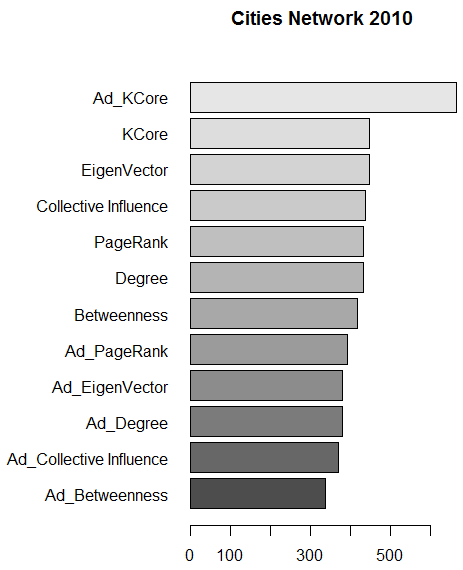
\includegraphics[width=1\linewidth]{city-network-metrics-2010}
					\label{fig:city-network-metrics-2010}
				\end{subfigure}%
				\begin{subfigure}{0.5\textwidth}
					\centering
					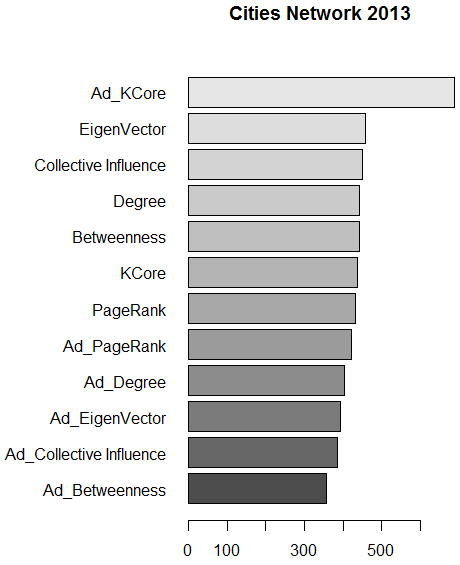
\includegraphics[width=1\linewidth]{city-network-metrics-2013}
					\label{fig:city-network-metrics-2013}
				\end{subfigure}
				\caption[Comparison of network metrics to identify for city networks]{Comparison of network metrics to identify the most effective method for networks of 2010 and 2013. Metrics are sorted by the lowest performing to the best performing from top to bottom. X-axis represents the number of node removals required to completely disintegrate the entire network whereas Y-axis represents the size of the biggest connected component in the network. Prefix \textbf{Ad} with different metrics represents the adaptive sampling variant.}
				\label{fig:city-network-metrics}
			\end{figure}
			
			\begin{figure}[H]
				\begin{subfigure}{0.5\textwidth}
					\centering
					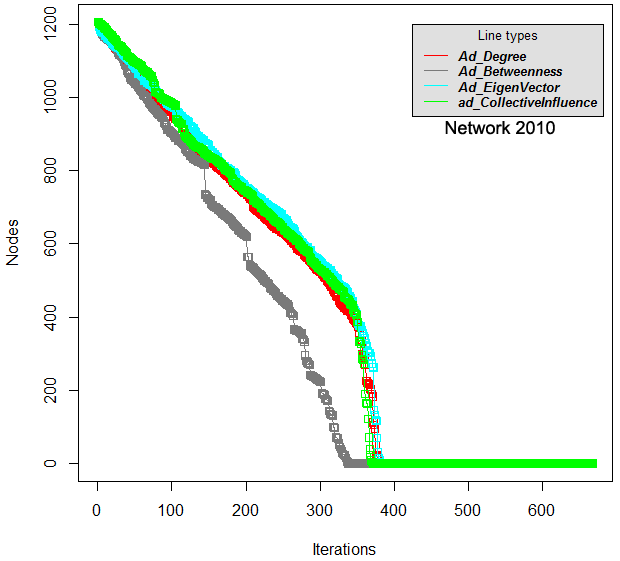
\includegraphics[width=1\linewidth]{city-network-dismantling-2010}
					\label{fig:city-network-dismantling-2010}
				\end{subfigure}%
				\begin{subfigure}{0.5\textwidth}
					\centering
					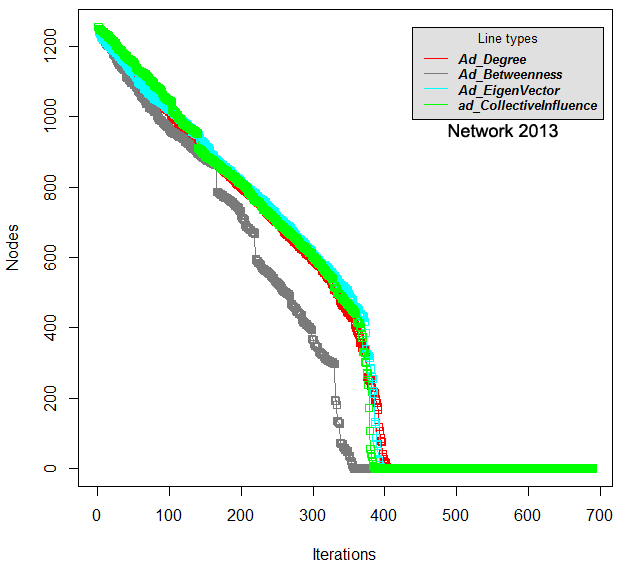
\includegraphics[width=1\linewidth]{city-network-dismantling-2013}
					\label{fig:city-network-dismantling-2013}
				\end{subfigure}
				\caption[Comparing the four best metrics to determine network connectivity]{Comparing the four best metrics to determine network connectivity. On x-axis is the number of iterations which a method took to dismantle the network; on y-axis is the number of remaining nodes in the largest component of the network. As seen, the Adaptive Betweenness heuristic outperformed the other methods by dismantline the network faster in both networks.}
				\label{fig:city-network-dismantling}
			\end{figure}
		
			\subsubsection{Cumulative city rankings}
			The importance of cities cannot be determined by a single metric because all Diversity, Strength and Centrality measures highlight the vitality of a city. These three metrics -- originally inspired by social network analysis -- have formed the basis of many research studies to quantify the role of cities in the world economy \cite{alderson2004,derudder2010,rozenblat2017}. As there's no order in which these metrics can be used, we propose a cumulative rank ($CR$) which combines all three to ensure an unbiased representation of various dimensions studied in this section. The cumulative rank is weighed equally by taking harmonic mean: $CR_i=\frac{n}{\sum_{i=1}^{n} \dfrac{1}{x}}$. The harmonic mean of a city $i$ given by $CR_i$ is calculated by using the rank of city $x$ for each of the three metrics ($n=3$) such that $x_1$, $x_2$ and $x_3$ represent the rankings in the three metrics. The cumulative rank ensures that the importance of a city is measured along all three dimensions, thus building a fair basis for interpretation of results.
	
		\subsection{Results}
		First and most important finding is the fact that on this real world network, neither a traditional, nor a state-of-art method proved to be the best in finding the most central nodes. The experiments on networks reveal that Adaptive sampling method of Betwenneess Centrality outperforms the other metrics in identifying the most central nodes.
	
			\subsubsection{Diversity}
			Figure \ref{fig:city-network-diversity} shows the diversity of cities in 2010 and 2013. The cities which are very close to the trend line have maintained their status from the year 2010 to 2013. Almost all the top cities like \textbf{Paris}, \textbf{New York} and \textbf{Tokyo} have shown this tendency which reflects that in terms of diversity, not much changed during the studied period. The cities which are far below the trend line have decreased in terms of diversity. Major cities affected in this way are \textbf{Frankfurt}, \textbf{Copenhagen}, \textbf{Stockholm} and \textbf{Rome}. Cities which are above the trend line such as \textbf{Milan}, \textbf{Geneva} and \textbf{Baltimore} have increased their diversity over the period and now have more connections to different cities. Cities of \textbf{Scandinavia} (like Copenhagen, Stockholm, or Goteborg) or cities of \textbf{South} (like Roma, Barcelona) mostly decreased while cities situated at the center like \textbf{Zurich}, \textbf{Geneva}, \textbf{Milano}, or \textbf{Mannheim} increased. Because of the crisis, networks have a tendency to concentrate in some geographic central cities, despite the observed exception of Frankfurt hosting the European central bank which had the opposite effect of weakening the city.
			
			Also interesting mention here are the cities of \textbf{Dubai} and \textbf{Abu Dhabi} which have also increased considerably representing growth in the Gulf region.
			
			\begin{figure}[H]
				\centering
				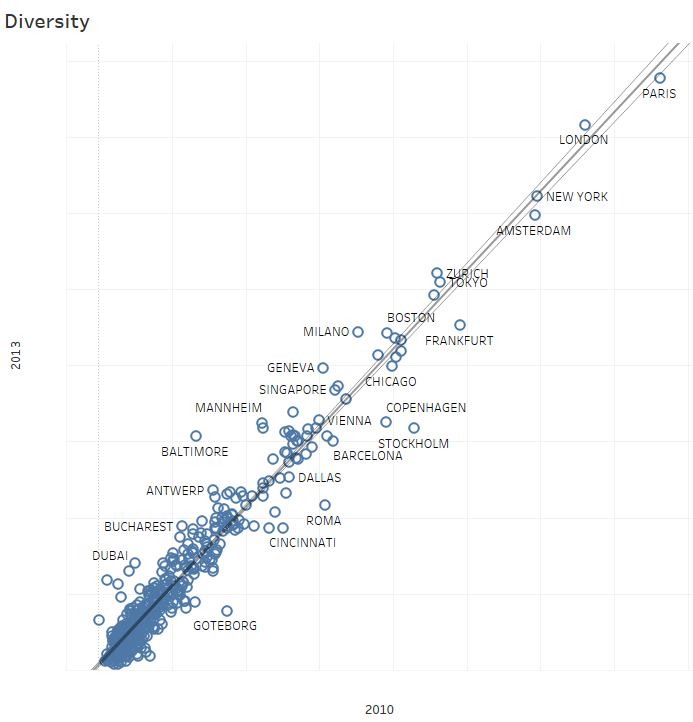
\includegraphics[width=0.8\linewidth]{city-network-diversity.png}
				\caption[Diversity plot of city networks]{Plotting \textit{Diversity} of cities in 2010 (x-axis) against 2013 (y-axis). The cities which are very close to the trend line have maintained their status. Cities below the trend line have decreased diversity from 2010 to 2013 whereas cities  above the trend line have increased diversity from 2010 to 2013.}
				\label{fig:city-network-diversity}
			\end{figure}
			
			\subsubsection{Strength}
			Figure \ref{fig:city-network-strength} shows the strength of cities in 2010 and 2013. Again, the cities which are close to the trend line have preserved their status over the years with some major cities like \textbf{Paris}, \textbf{New York} and \textbf{Amsterdam} showing this tendency. The cities which are below the trend line have decreased in terms of strength. Major cities affected are \textbf{Moscow}, \textbf{London}, \textbf{Frankfurt} and \textbf{Hong Kong} which are among the main financial centres in their own regions and it is interesting to see their decrease in strength. Cities which are above the trend line like \textbf{Philadelphia}, \textbf{Milan}, \textbf{Chicago} and \textbf{Tokyo} have increased their strength by increasing the weight of their connections to other cities. It is interesting to see a couple of cities from \textbf{China} (Beijing and Shanghai) in this list, as well as cities from \textbf{Brazil} (Sao Paulo) and \textbf{Romania} (Bucharest).
			
			\begin{figure}[H]
				\centering
				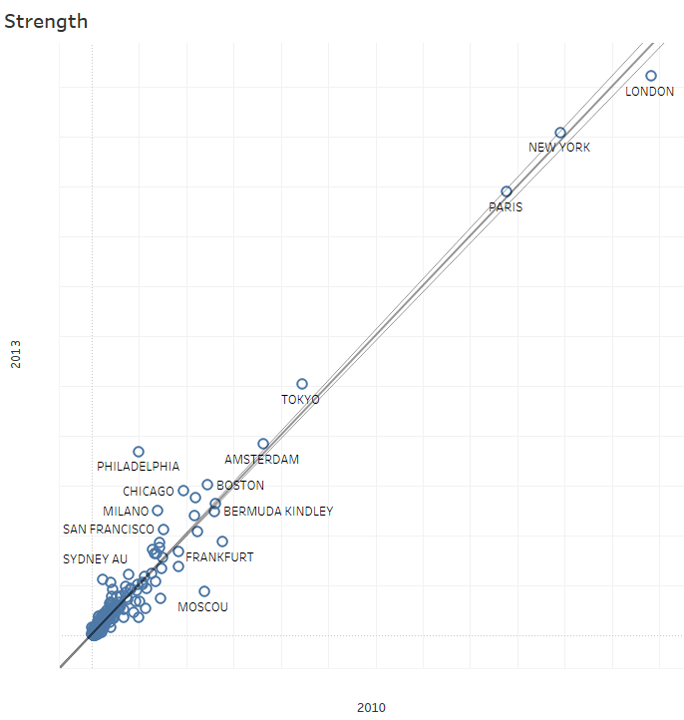
\includegraphics[width=0.8\linewidth]{city-network-strength}
				\caption[Strength plot of city networks]{Plotting \textit{Strength} of cities in 2010 (x-axis) against 2013 (y-axis). The cities which are very close to the trend line have maintained their status. Cities below the trend line have decreased strength from 2010 to 2013 whereas cities  above the trend line have increased strength from 2010 to 2013.}
				\label{fig:city-network-strength}
			\end{figure}
			
			\subsubsection{Centrality}
			Figure \ref{fig:city-network-centrality} shows the centrality of cities in 2010 and 2013. The enlarged image on the right shows only the top part for increased readability. The cities which are close to the trend line have similar centrality values for the two years with notable cities like \textbf{Frankfurt}, \textbf{Brussels}, \textbf{Vienna}, \textbf{Chicago} and \textbf{Saint Petersbourg}. Some of the cities which have decreased in terms of centrality are \textbf{Goteborg} (Sweden), \textbf{Graz} (Austria), \textbf{Salt Lake City} (USA) and \textbf{Kuwait}. Cities which have increased centrality include \textbf{Dubai} (UAE), \textbf{Salzburg} (Austria), \textbf{Baltimore} (USA) and \textbf{Penang} (Malaysia). It is interesting to note that there are a couple of cities each from \textbf{Russia}, \textbf{Korea}, \textbf{China} and \textbf{United Arab Emirates} in this list. \textbf{Eastern Europe} is also well represented by \textbf{Akrotiri} (Santorini in Cyprus), \textbf{Gdansk} (Poland), \textbf{Tirana} (Albania) and \textbf{Vilnius} (Lithuania) showing the emerging trend of these countries and regions.
			
			\begin{figure}[H]
				\centering
				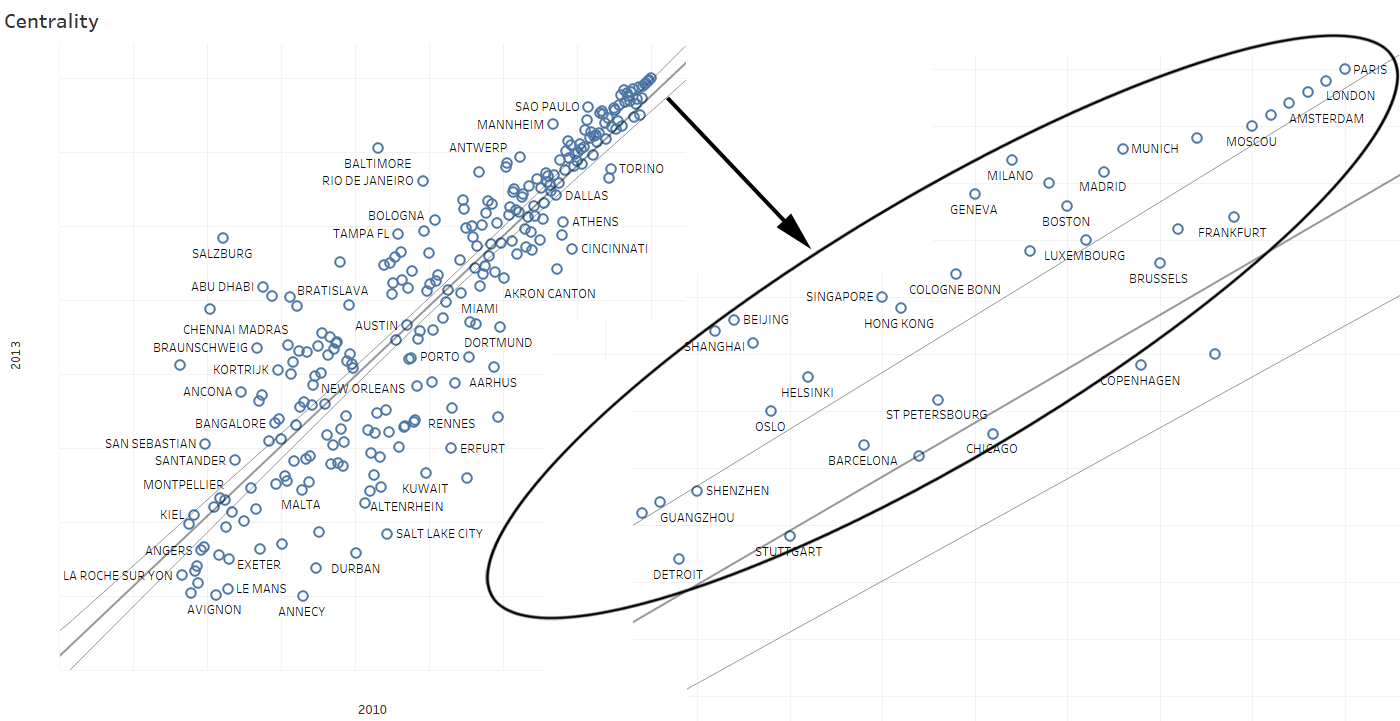
\includegraphics[width=0.8\linewidth]{city-network-centrality}
				\caption[Centrality plot of city networks]{Plotting \textit{Centrality} of cities in 2010 (x-axis) against 2013 (y-axis). The image on the right enlarges the top cities. Again the cities which are very close to the trend line have maintained their status. Cities below the trend line have decreased centrality from 2010 to 2013 whereas cities above the trend line have increased centrality from 2010 to 2013.}
				\label{fig:city-network-centrality}
			\end{figure}
			
			Figure \ref{fig:city-network-cumulative-centrality} shows the cumulative rank of cities in 2010 and 2013. The enlarged image on the right shows the top cities based on the cumulative ranking of the cities. The world’s top cities can easily be identified with most of the top performers in 2010 retaining their position in 2013. Cities like \textbf{Paris}, \textbf{London}, \textbf{New York} and \textbf{Tokyo} have fairly stable positions in both years. It means that despite some smooth changes in each of the dimensions, largest cities main- tain a very stable position. \textbf{Milan}, \textbf{Geneva}, \textbf{San Francisco} and \textbf{Baltimore} have improved their standings where cities like \textbf{Stockholm}, \textbf{Frankfurt}, \textbf{Copenhagen} and \textbf{Barcelona} have dropped their position.
			
			\begin{figure}[H]
				\centering
				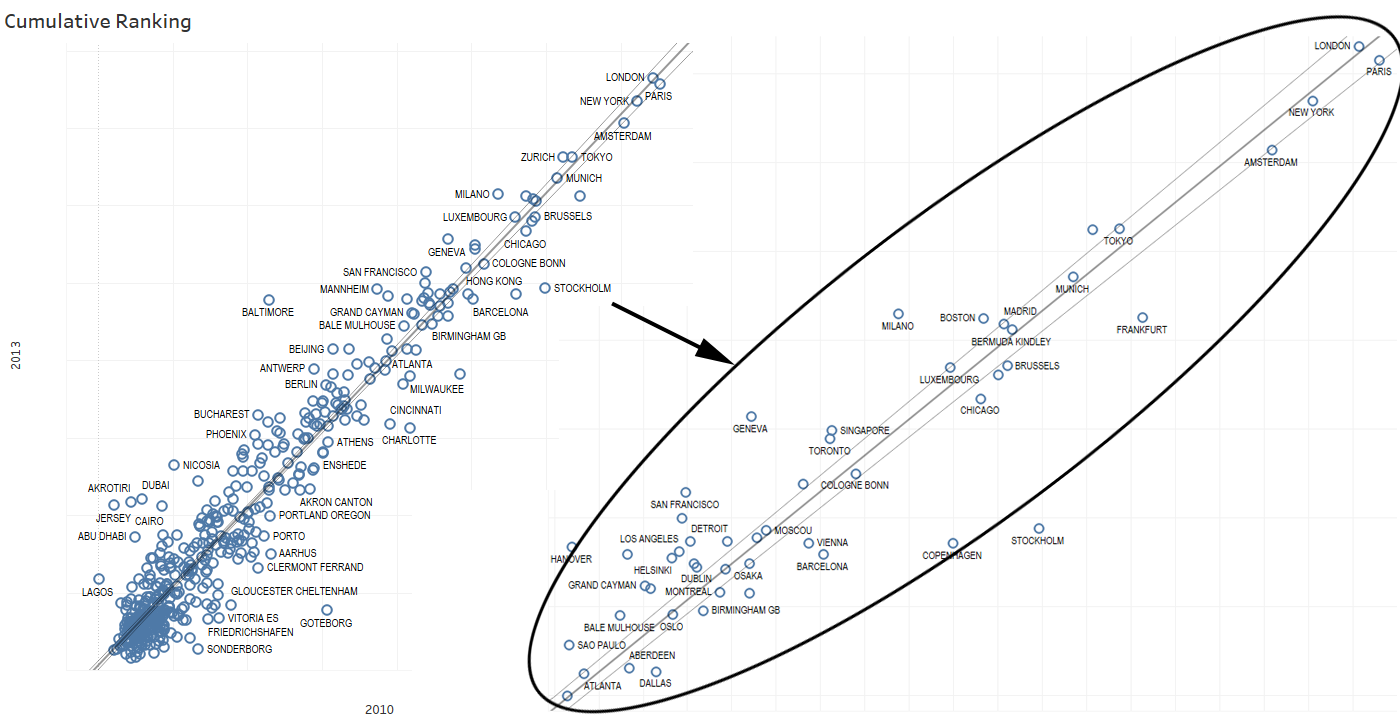
\includegraphics[width=0.8\linewidth]{city-network-cumulative-centrality}
				\caption[Cumulative ranking of cities for 2010 and 2013]{Plotting \textit{Cumulative Rank} of cities in 2010 (x-axis) against 2013 (y-axis). The image on the right shows the top cities zoomed-in. Again the cities which are very close to the trend line have maintained their status. Cities below the trend line have decreased the cumulative rank from 2010 to 2013 whereas cities above the trend line have increased cumulative rank from 2010 to 2013.}
				\label{fig:city-network-cumulative-centrality}
			\end{figure}
		
		Our findings are summarized in Figures \ref{fig:city-networks-top-cumulative-map}, \ref{fig:city-networks-top-positive-cumulative-map}, and \ref{fig:city-networks-top-negative-cumulative-map} in Appendix \ref{chp:figures} on a globe for better visualization.
		
		Cities which have been affected the most by the changes in global economic development of multinational firms from 2010 to 2013. Figure \ref{fig:city-networks-top-cumulative-map} shows the top 25 cities from the years 2010 and 2013. Three regions clearly stand out from the geographical perspective, North America, Western Europe and Eastern Asia. Moscow (Russia) and Sydney (Australia) are also among the top cities in the world. Cities from South America, all of Africa, South Asia and the Gulf are interestingly not part of this list.
		
		Figure \ref{fig:city-networks-top-positive-cumulative-map} and \ref{fig:city-networks-top-negative-cumulative-map} show the cities with the most positive and negative impact over the studied period.
		
		Comparing these cities with the top cities reveal how the world economy is changing in the context of multinational firms. Detailed results of all three metrics are given in section \ref{sec:appendix-B-city-networks} of Appendix \ref{chp:tables}. We discussed insights and details of a few cities from both the sets of cities with the highest positive and negative change in supplementary comments (Appendix \ref{sec:appendix-B-city-networks}). There are several factors that result in this change such as global economics, urban development, regional policies, international politics and social capital. Besides the general crisis affecting the whole cities’ network by a concentration in most of the former dominant regions, and the rise of new cities in emerging countries, the main factor explaining why some cities faced the crisis better than others can be found in their specialization in some growing economic sectors.
		
	The key observation from the above experiment from influence mining perspective is that albeit an abundance of methods and techniques and state-of-art being furthered each year, one method cannot qualify to be a gold standard in all real-world cases. Moreover, we observed that a primitive topological method such as Betweenness can also outperform state-of-art measures in certain cases.
	
	This finding leads us to take a collective approach instead of looking for one particular heuristic. The key question we aim to answer is if we can learn from multiple seed selection methods and train a single influential node identifier. The experiment discussed in next section is an attempt to use supervised machine learning, a data mining technique to achieve this objective.
	
%	\newpage
	
	%%%%%%%%%%%%%%%%%%%%%%
	%%% Experiment - 3 %%%
	%%%%%%%%%%%%%%%%%%%%%%
	\section{Influence maximization in complex networks through supervised machine learning}
	\label{sec:inf-max-machine-learning}
	Previous experiments evidently establish that a conventional way of inventing an algorithm to solve the influence mining problem work only for a particular set of use cases. Such techniques have to be evaluated before applying on a real-world use case. We propose that the answer lies in using data mining technique called supervised machine learning.
	
	The applications of machine learning emerging in every field is no surprise. However, the influence maximization domain surprisingly faces some scarcity. Among the few studies that exist, the prominent publications are quite specific, and often specific to social networks.
	
	Goyal et. al. \cite{goyal2010} focus on predicting the probability with which a user will propagate influence to individual neighbours in a network. Their proposed solution scans the log of user actions only twice and are able to learn three types of probabilistic models: static, continuous time and discrete time. Secondary contribution in this study is predicting the influence time. Finally, the results prove that continuous probabilistic model works better than static model. A common disadvantage with this solution is that it requires not only the network information, but also the log of actions performed by the nodes in the network. In addition to this, scanning the action logs twice can also be expensive in some situations as these logs tend to be huge in size.
	
	Guille et. al. \cite{guille2013} demonstrate how predictive analytics can be used to predict diffusion cascades in a social network. Their proposed model, T-BaSIC does not assume a fixed diffusion probability, but rather a time-dependent function. This temporal diffusion model is used create time series to describe how a topic originated and spread in a Twitter network in a closed set of users. The authors trained multiple classifiers to learn parameters for diffusion function, and opted Bayesian logistic regression classifier to define the diffusion function. The results show that int the information diffusion process, initially the volume of tweets is high against a topic, and then lowers with time following a wave pattern. Conclusively, the T-BaSIC method reduces the overall diffusion prediction error by 32.75\% in comparison with 1-time lag model proposed by Yang \cite{yang2011}.
	
	Zanin \cite{zanin2016} discusses the significance of applying data mining techniques in complex networks. The authors describe how data mining techniques can make use of structural patterns of individual nodes as well as whole network. Excerpts from this article are widely reflected in experiments we propose in the supervised machine learning experiment.
	
	Albeit these attempts, to the best of our knowledge there is lack of any published work which solves the influence mining problem using supervised machine learning on a complex networks of varying structural properties. These properties are thoroughly discussed in next sub-section.
	
		\subsection{Experiment settings}
		The primary focus is to provide a novel approach to identify influential nodes in complex networks. We attempt to develop a method which is widely applicable to networks with varying structural and nodal properties. The aim of this experiment is neither to invent a new machine learning algorithms, nor make performance comparisons between the existing machine learning algorithms.
		
			\subsubsection{Training data sets}
			The experiments discussed primarily consist of openly available real graphs as well as synthetically generated graphs. Moreover, unlike majority of studies, which use network data, user attributes, action logs and other information, we only use network’s structural properties that can be calculated by $G=(V,E)$, where $V$ is a set of vertices or nodes in the graph $G$, while $E$ is the set of edges or links connecting these vertices.
			
			Since it is vital to have variety in our data, we used networks from various domains, different sizes and different structural properties. The networks used in this study come from three sources:
			
			\begin{enumerate}
				\item Synthetic networks: We drew 6 random samples for each of the following types of complex networks using Igraph library \cite{igraph2006,barabasi1999,holme2002b} ranging from sizes: 10, 15, 20, 25, 30, 35, 40, 45, 100, 200, 300, 400, 500, 600, 700, 800, 900, 1000, 1500, and 2000. Thus creating 120 complex networks (scale free and small-world).
				
				\item Public networks: We used five of the frequently cited networks from various domains like biology and social networks, which are available online. Namely Zachary karate club \cite{zachary1977}, World trade \cite{smith1992}, Nematode \cite{white1986}, Political blog \cite{adamic2005} and Yeast protein \cite{jeong2001}.
				
				\item Extracted networks: we extracted two networks described as follows:
				
				\begin{itemize}
					\item Influence citations: network of paper citations on topic of influence mining till 2016. The data set was constructed by collecting a corpus of research articles on various topics of Influence mining. Each node in this network represents a unique article, while the edges represent citations between these articles.
					
					\item Twitter: network of users linked on Twitter, collected using snowball sampling. Starting with a reference user account (ID: seekme 94) in the Twitter network, a subset of Twitter’s network was extracted, in which each node is either a direct connection of reference account, or a connection at a distance of 1 degree. The edges represent interconnections between these nodes. The reference node was finally removed from the network.
				\end{itemize}
			\end{enumerate}
			
			This gives us a total of 367 networks for training and validation. Table \ref{tab:inf-max-machine-learning-training-graphs} shows basic statistics for all the real networks used for training the model. APL is Average Path Length, $\alpha$ is Power-law coefficient, CC is clustering coefficient and Avg. Deg is Average Degree. The variation in size of the networks, average path length, power law coefficient, clustering coefficient and average degree demonstrates how we have captured different network level structural properties for our training data set.
		
			\begin{table}[h]
				\centering
				\begin{tabular}{|l|l|l|l|l|l|l|}
					\hline
					\textbf{Network} & \textbf{Nodes} & \textbf{Edges} & \textbf{APL} & \textbf{$\alpha$} & \textbf{CC} & \textbf{Avg. Deg} \\ \hline
					Karate club        & 34   & 78    & 2.4 & 2.12 & 0.256 & 4.6  \\ \hline
					World trade        & 80   & 1000  & 1.7 & 2.56 & 0.460 & 25   \\ \hline
					Nematode           & 297  & 2359  & 2.5 & 3.29 & 0.181 & 15.9 \\ \hline
					Political blog     & 1222 & 19089 & 2.7 & 3.89 & 0.226 & 31.2  \\ \hline
					Yeast protein      & 1458 & 3941  & 6.8 & 3.24 & 0.052 & 5.4 \\ \hline
					Influence citation & 1254 & 1993  & 3.8 & 2.35 & 0.057 & 3.2  \\ \hline
					Twitter            & 894  & 2060  & 4.9 & 4.60 & 0.017 & 4.6  \\ \hline
				\end{tabular}%
				\caption{Real Networks used for training machine learning models}
				\label{tab:inf-max-machine-learning-training-graphs}
			\end{table}
			
			\subsubsection{Test data sets}
			In order to test the final model, following networks from various domains were used. Again, variation in their nodal as well as structural properties can be observed in Table \ref{tab:inf-max-machine-learning-test-graphs}. All these networks are also frequently used in different experiments and cited in the literature.
			
			\begin{table}[h]
				\centering
				\begin{tabular}{|l|l|l|l|l|l|l|}
					\hline
					\textbf{Network} & \textbf{Nodes} & \textbf{Edges} & \textbf{APL} & \textbf{$\alpha$} & \textbf{CC} & \textbf{Avg. Deg} \\ \hline
					Author   & 379    & 914    & 6.0 & 3.36 & 0.431 & 4.8  \\ \hline
					ITA 2000 & 3304   & 67195  & 4.0 & 1.69 & 0.249 & 40.7 \\ \hline
					AS-CAIDA & 26475  & 53381  & 3.9 & 2.09 & 0.007 & 4.0  \\ \hline
					JDK      & 6434   & 150985 & 2.1 & 2.01 & 0.011 & 46.9 \\ \hline
					Wordnet  & 145145 & 656230 & 5.5 & 2.47 & 0.096 & 9.0  \\ \hline
				\end{tabular}
				\caption{Real Networks used for testing classification models}
				\label{tab:inf-max-machine-learning-test-graphs}
			\end{table}
			
			\begin{itemize}
				\item Author NetScience: a coauthorship network of scientists working on network theory and experiment \cite{newman2006b}.
				
				\item ITA 2000: a reduced version of Air Transport network representing connections between airports through direct flights \cite{rozenblat2008}.
				
				\item AS-CAIDA: network of autonomous systems of the Internet connected with each other from the CAIDA project, collected in 2007 \cite{ascaida}.
				
				\item JDK Dependencies: a network of class dependencies in Java Development Framework v1.6 \cite{jdk}.
				
				\item Wordnet: a lexical network of English words in which each node represents a word and edges are relationships like synonym and antonyms \cite{fellbaum2012}.
				
			\end{itemize}
			
			
			\subsubsection{Machine learning models}
			In a relatively latest review paper, Fernandez et al. \cite{fernandez2014} argued that the real world classification problems do not require too many machine learning models after comparing 179 classifiers on 121 data sets. Analyzing the results of the best and worst performing models from different families, we used the following models for our experiment:
			
			\begin{enumerate}
				\item Logistic regression: Generalized Linear Model by Dobson \cite{dobson2018}, abbreviated as \textbf{GLM}.
				
				\item Decision Trees and Rule-Based: Recursive partitioning by \cite{breiman1984}, abbreviated as \textbf{RPart} and \textbf{C5.0}, an extended version of original C4.5 model by \cite{quinlan1993}. 
				
				\item Support Vector Machines: \textbf{SVM} model using Gaussian kernel from popular LibSVM library \cite{chang2011}.
				
				\item Boosting: Random Forests by \cite{breiman2001}, abbreviated as \textbf{RForest} and eXtreme Gradient model by \cite{chen2016}, abbreviated as \textbf{XGBoost}.
			\end{enumerate}
			
			From the data sets, the target variable tells whether the node was identified as influential by optimal/Greedy algorithm or not. The models are evaluated using accuracy measure, a standard way to compare the performance of machine learning models (see Equation \ref{eq:inf-max-accuracy}).
			
			\begin{equation}
				\label{eq:inf-max-accuracy}
				Accuracy=\frac{TP+TN}{TP+FP+TN+FN}
			\end{equation}
			
			Where $TP$ (true positives): number of nodes which were correctly classified as influential. $TN$ (true negatives): number of nodes which wore correctly classified as non-influential. $FP$ (false positive): number of nodes which were incorrectly classified as influential. $FN$ (false negative): number of nodes which were incorrectly classified as non-influential.
			
			\subsubsection{Modest computing power}
			The experiments were all conducted on a workstation laptop, consisting of quad-core CPU running at 3.6GHz in combination with 16GB RAM and 512GB storage. The modest computing power demonstrates that the solution does not require high-speed computational stations.
			
		\subsection{Influential node identification}
		The first step to train supervised machine learning models is to identify influential nodes in training data.
		
			\subsubsection{Influence maximization}
			In order to guarantee that the nodes we label as influential, in fact are influential, we used an exhaustive search to find the optimal solution (NP-hard) for networks of size less than 50 nodes (see Algorithm \ref{alg:influence-maximization}), and Hill-climbing based Greedy solution for larger networks (see Algorithm \ref{alg:influence-greedy-solution}). Opting for greedy algorithm was the next best method possible after an exhaustive search because finding the optimal solution for larger graphs is practically impossible in realistic time.
			
			\subsubsection{Influence test}
			In order to quantify the influence of a node, multiple methods exist, including diffusion test under both LT and IC models, resilience test \cite{cohen2000} which quantifies the network breakdown after a set of nodes is removed. Since the resilience test does not require any data other than network information, therefore this study uses resilience test as other similar studies \cite{holme2002,morone2015}. 

			Conventionally, the resilience test is a network decomposition function. In discrete time steps, one node (or a set of similar nodes) is removed from the network and we compute the largest connected component remaining in the network. This iteration is repeated until network completely decomposes. The quicker a method decomposes the network, the better its performance. In the underlying experiment, instead of single node a batch of $k$ nodes is removed in exactly one iteration and the size of the biggest connected component is measured.
			
			\subsubsection{Budget}
			Budget, or the number of influential nodes to identify, was fixed to 10\% for networks with nodes less than 50 and, 2.5\% for all other networks.
			
		\subsection{Training features}
		For a machine learning model to perform optimally, feature selection and data transformation are the key steps. For this experiment, we carefully chose a number of nodal and network level traits as training feature set:
		
		\begin{enumerate}
			\item Network traits: out of the numerous network traits which explain the structure of a network. Each trait has merits and demerits. This study chose the following 11 most commonly used network level traits as input to the training model, i.e. Network size, Edges, Highest Degree, Average Degree, APL, Clustering Coefficient, Diameter, Density, Average Distance, Number of Triads and Assortativity.
			
			\item Node centrality traits (see \ref{sec:related-seed-selection}): these traits define how central to the network certain node is. We included these five node centrality traits: Degree, Betweenness, Closeness, Eigenvector centrality and Eccentricity.
			
			\item Other heuristics (see \ref{sec:related-seed-selection}): in this category we picked three heuristics; we included Coreness due to its performance in identification of influential nodes as claimed by \cite{kitsak2010}, \cite{bae2014}. Batagelj proposed an algorithm with complexity $O(n)$ to compute coreness \cite{batagelj2003}. Secondly, we add Pagerank, the popular ranking algorithm developed by Google Inc. \cite{pagerank1999}. Third and last one is Collective Influence, because of two particular reasons: it identifies weak nodes, which act as bridges between strong influences; it is scalable to large networks. All of these heuristics exploit the topological information in order to grant ranking to a particular node.
		\end{enumerate}
		
		It is important to note that since not all attributes have bounded values between standard ranges; we normalized the unbounded attributes to standardize all data.
		
		\subsection{Results}
		First, we look at how each model performs on different sizes of networks. An ideal model should perform consistently well irrespective of size of the network. We then average the accuracy of each model on all the graphs in validation set.
		
		Figure \ref{fig:machine-learning-model-accuracy-by-size} illustrates the accuracy of classification models over different sizes of validation networks, horizontal axis represents size and vertical axis accuracy of models. Average accuracy is given in Figure \ref{fig:machine-learning-model-accuracy}.
		
		\begin{figure}[H]
			\centering
			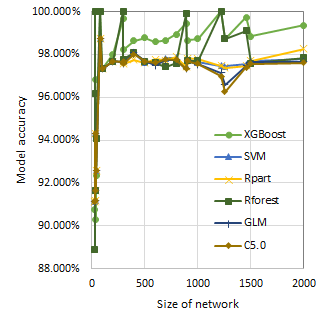
\includegraphics[width=0.7\textwidth]{machine-learning-model-accuracy-by-size}
			\caption[Accuracy of classification models]{Accuracy of classification models on various sizes of networks in validation set. Size of the networks are on horizontal axis, while the accuracy of each model on these sizes are on vertical axis.}
			\label{fig:machine-learning-model-accuracy-by-size}
		\end{figure}
		
		From Figure \ref{fig:machine-learning-model-accuracy}, it is evident that XGBoost has the highest accuracy overall on varying sizes of networks. We also observe that the performance of all models in small graphs is variable. However, XGBoost still outperformed other models on small networks. Therefore, we selected XGBoost based on its performance in comparison with other supervised machine learning models to evaluate networks in test data set.
		
		\begin{figure}[H]
			\centering
			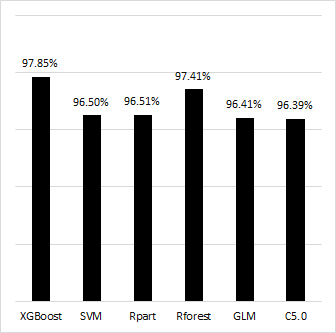
\includegraphics[width=0.5\textwidth]{machine-learning-model-accuracy}
			\caption[Average model accuracy on validation set]{Average accuracy of classification models on all networks in validation set}
			\label{fig:machine-learning-model-accuracy}
		\end{figure}
		
		The key objective of this study is to find out if a machine learning algorithm can outperform other heuristic methods in discovering influential nodes in networks of various sizes and structural properties. In order to test our hypothesis, we pass all the test networks to the XGBoost model to identify $k$ most influential nodes. The output obtained from the model is a probability against each node, which quantifies how strongly the model classified that particular node as influential. We pick the set of 5\% $k$ nodes of the highest probabilities and perform resilience test on the test networks. Resilience test is destructive; it is used to measure how much a network decomposed when a set of nodes is removed. After removing $k$ influential nodes identified by the model, we calculate the size of the largest connected component in the remaining network. Therefore the method, which identifies $k$ nodes that results in higher decomposition of the network qualifies as a better performer.
		
		The results shown in Figure \ref{fig:machine-learning-model-resilience} illustrate that the XGBoost model performed very well when compared with commonly used heuristics. In this figure, "size" on x-axis represents the number of nodes in the original test network, while other bars represent how large the network remained after removing 5\% $k$ influential nodes. Best results are highlighted with bold-italic text in the figure.
		
		\begin{figure}[H]
			\centering
			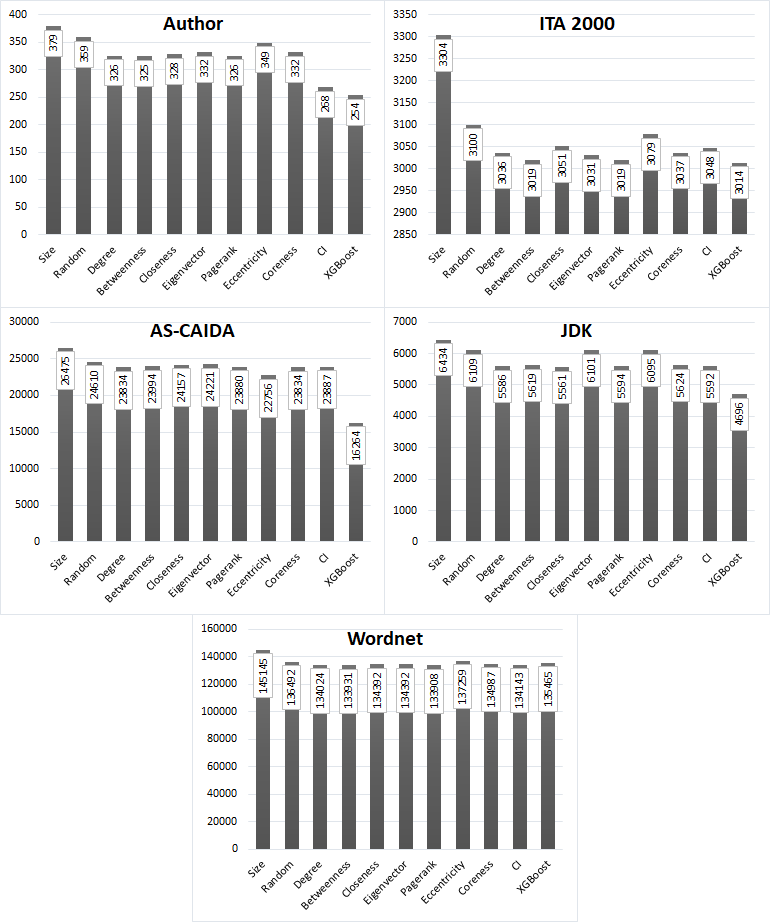
\includegraphics[width=0.7\textwidth]{machine-learning-model-resilience}
			\caption[Classification model vs other influence methods]{Comparison of influence mining methods against classification model. On x-axis are the methods under comparison. On y-axis is the number of nodes in largest component after removing $k$ nodes from the network}
			\label{fig:machine-learning-model-resilience}
		\end{figure}
		
			\subsubsection{Author}
			This is the smallest of all test networks. XGBoost model collapsed the largest connected component in the network to 254 nodes (removing 19 nodes).
			
			\subsubsection{ITA 2000}
			XGBoost showed best results with the size of largest connected component to 3014 nodes, but only marginally better than Pagerank and Betweenness centrality which reduced the size of the largest connected component to 3019 nodes (removing 165 nodes).
			
			\subsubsection{AS-CAIDA}
			A relatively large network, where XGBoost (16264 nodes) dominated other methods with significant margin. Eccentricity (22756 nodes) is the next best with a considerable difference (removing 1324 nodes).
			
			\subsubsection{JDK}
			Similar results with XGBoost (4696 nodes) can be observed (removing 322 nodes). It is interesting to note that in this particular network, Eigenvector centrality and Eccentricity are only slightly better than random method. Thus indicating that centrality based methods may not perform better universally.
			
			\subsubsection{Wordnet}
			Results on this -- largest -- network differs from others for XGBoost. The method that produced best results turned out to be Pagerank, which dismantled the network down to 133908 nodes on removing 7257 nodes. Followed closely by Betweenness (133931 nodes). The XGBoost model disappointingly fell below all other methods except Eccentricity and Random.
			
		Analyzing the results, although the XGBoost model stands on top, analysis on next best also reveals that there is no clear runner up method. For example, CI shows impressive results on Author network, but does not hold this performance on other networks. Table \ref{tab:inf-max-machine-learning-ranking} lists the influence methods and ranks using average ranking method. As observable, CI has 2nd rank in Author network, but fails on other networks; Betweenness and Pagerank perform equally well on ITA 2000, but do not hold this position for other networks; likewise, Eccentricity is impressive on AS-CAIDA network, but performs almost similar to random method on other networks.
		
		This observation also validates that the use of heuristic methods to identify influential nodes is highly dependent of various nodal and structural attributes and thus perform differently on different networks. Therefore, no heuristic can be considered as a generic algorithm to accurately identify influential nodes in a variety of complex networks.
		
		Another observation is that not all networks decompose with the same rate. For example, ITA 2000 network proved highly resilient by sustaining a size of 3014 (91\%) after removing influential nodes. On the other hand, AS-CAIDA reduced to 16264 (61\%). It is also evident that random methods perform poorly, as indicated by various other studies.
		
		Finally, coming to the case where machine learning model failed on Wordnet. A clear reason for such poor results is that in the training data, we had not provided the model with any network of such size. Here we find a learning limitation of the model, i.e. without providing ample data set which consists of all sizes of networks, the machine learning model fails to identify target nodes. Not only that, but as we observe in the results, it may perform about same as random selection.
		
		\begin{table}[h]
			\centering
			\begin{tabular}{|l|l|l|l|l|l|}
				\hline
				\textbf{Network} & \textbf{Author} & \textbf{ITA 2000} & \textbf{AS-CAIDA} & \textbf{JDK} & \textbf{Wordnet} \\ \hline
				\textbf{Random}       & 10  & 10  & 10  & 10 & 9   \\ \hline
				\textbf{Degree}       & 4.5 & 5   & 3.5 & 3  & 3   \\ \hline
				\textbf{Betweenness}  & 3   & 2.5 & 7   & 6  & 2   \\ \hline
				\textbf{Closeness}    & 6   & 8   & 8   & 2  & 5.5 \\ \hline
				\textbf{Eigenvector}  & 7.5 & 4   & 9   & 9  & 5.5 \\ \hline
				\textbf{Pagerank}     & 4.5 & 2.5 & 5   & 5  & 1   \\ \hline
				\textbf{Eccentricity} & 9   & 9   & 2   & 8  & 10  \\ \hline
				\textbf{Coreness}     & 7.5 & 6   & 3.5 & 7  & 7   \\ \hline
				\textbf{CI}           & 2   & 7   & 6   & 4  & 4   \\ \hline
				\textbf{XGBoost}      & 1   & 1   & 1   & 1  & 8   \\ \hline
			\end{tabular}
			\caption{Ranking comparison between the influence methods and classification model}
			\label{tab:inf-max-machine-learning-ranking}
		\end{table}
		
		The experiments and results not only validate the proposal by outperforming various conventional and state-of-art methods, but take us a step ahead in terms of prerequisites. The model which was trained for this study was based on synthetic networks, combined with some openly available network data sets. The classification model outperformed the competing methods in tested real world networks except in one instance. While machine learning can certainly help in various applications, it is important to note that training the model is computationally much more expensive than any other heuristic in comparison. It is assumed that anyone applying this solution aims to reuse the model on various networks, and multiple times. For simple one-time applications, the solution is still valid in terms of performance, but has a high computation overhead. Therefore, one of the key areas of optimization is selecting the right set of features which reduces the overall complexity while maintaining the high performance achieved.
		
		Following are the key finding from the above experiment:
		\begin{itemize}
			\item Machine learning is a plausible solution to identify influential nodes. Moreover, it can learn from synthetic networks and thus does not inherently require obtaining training set from variety of sources.
			
			\item The computation cost of learning a model is high, given that structural and nodal attributes have to be calculated for each network, as well as label the influential nodes via a highly efficient algorithm like Greedy.
			
			\item The method cannot be scaled without enhancing the training data first on large networks. Thus leading us to a case of deep learning on Big data.
			
			\item Finally, in order to pass target network to the model, all the meta features have to be also calculated for the target network. Even if all such features are calculated in linear time, the total time complexity will be $O(n*c)$, where $c$ is the number of features. Hence the technique cannot be scaled without comprehensive feature pruning.
		\end{itemize}	
		

	\section{Summary}
	\label{sec:inf-max-summary}
	The problem of Influence Maximization is NP-hard. However, because this function is both monotone and sub-modular, a Greedy solution can solve it with an approximation guarantee of 63\%. Most of the stat-of-art solutions are an extension or variants of this approach. Since Greedy solution scans the entire network from fresh perspective in each iteration, it is generic and can be used for all complex networks irrespective of their structural properties. Greedy solution suffers scalability problem due to its quadratic time complexity, thus leaving an open research question.
	
	%Real complex networks are all unique, but their properties can be mimicked within certain margin of error in synthetic networks. Such networks are a good way to study and benchmark the original networks which they replicate.
	
	Empirical analysis of various seed set selection methods confirms that there are structural dissimilarities between networks even from within the same domain. Social networks are all scale-free and small world, but still one influence method is effective on a particular social network, while fail on another one.
	
	There are various heuristics and techniques with claims to outperform other methods on a chosen set of networks, but even a well presented state-of-art method cannot guarantee consistency on all kinds of networks.
	
	In the absence of an ideal influence maximization method, machine learning is a suitable alternate solution to train a corpus of different networks on several seed selection methods and be used for a broader spectrum of networks than one particular method offers. Moreover, resilience test can also be used as a benchmark method to quantify the influence of a node or a set of nodes in a network alike influence test. Lack of use of resilience in literature spots a major research gap. \\
	
The experiments discussed in this chapter have revealed that due to dissimilarities in structure of different complex networks, it is not trivial to devise a general purpose algorithm which can perform uniformly better on all of them. Secondly, existing methods have been fixed in the way the influence process converges, i.e. budget given to identify number of nodes. Finally, a major research gap exists where researchers either use influence test, or resilience test to benchmark a method. We believe there is need for a framework which addresses these deficiencies.


	\chapter{The Influence Mining Framework}
\label{chp:inf-framework}
Influence Maximization has been proven as holy grail specially for viral marketing applications, thus attracting more than a handful of researchers who have proposed a wide variety of techniques, which are all applicable based on the nature of network they are applied to. However, Thorough analysis of the influence mining problem suggests that due to inherent constraints and network dynamics, it is not possible to suggest an ideal method or technique which is both realistic as well as optimal on all complex networks. This problem is accurately illustrated in a recent paper \cite{arora2017}. The authors show that if Quality, Efficiency and Memory consumption are three criteria to decide which algorithm best solves the influence maximization problem, then all the available state-of-art methods either fulfill one or two criteria. An algorithm which satisfies all three does not yet exist (see Figure \ref{fig:state-of-art-im-methods}\cite{arora2017}). One of the major reasons -- as discussed in Chapter \ref{chp:inf-max} -- behind this bottleneck is the structural variety in complex networks.

\begin{figure}[h]
	\centering
	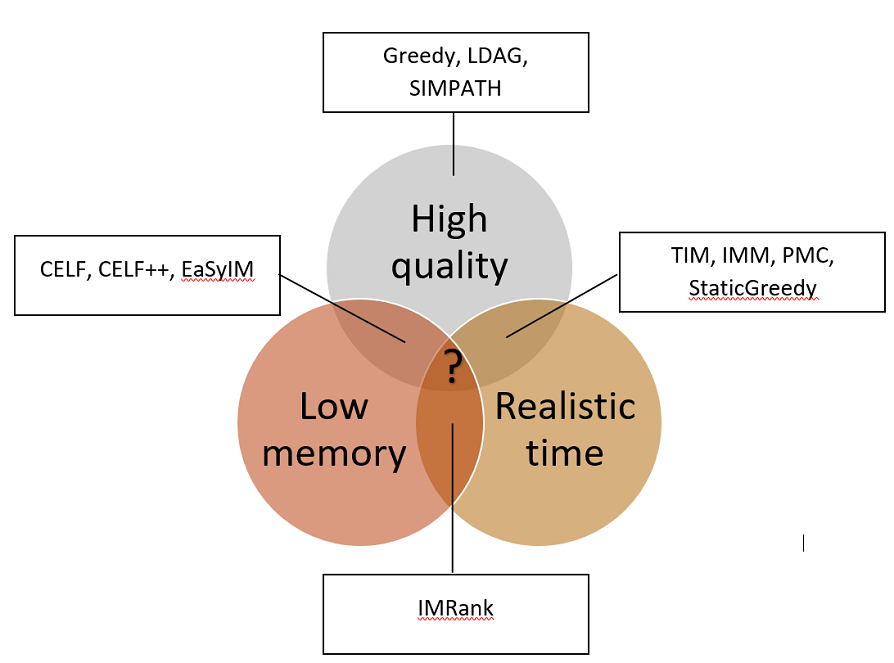
\includegraphics[width=0.7\textwidth]{state-of-art-im-methods}
	\caption[Deficiency in current state-of-art methods]{Several state-of-art methods and their primary objectives. The question mark denotes that no method exists to target all three criteria.}
	\label{fig:state-of-art-im-methods}
\end{figure}


	\section{Limitations of State-of-the-Art Methods}
	\label{sec:inf-framework-statofart-limitation}
	
		\subsection{Customary stoppage criteria}
		\label{subsec:inf-framework-stop-criteria}
		In lieu of an ideal influence maximization solutions, the applications are forced to adopt one algorithm. It is realistically challenging to apply one technique not only on a specific type of network, but also for varying use cases.
		
		First example in this regard is seasonal marketing campaigns. A business launching a new seasonal product will have a short time window to market and propagate their product before the competition launches more options, or the trend wears out. In this case, the business may allocate high budget, and may also overlook the magnitude of gain. However, the \textit{time} is real constraint and after the given window is passed, more efforts to maximize their influence will have significantly less gain against the effort put.
		
		In a different scenario, consider an automobile business introducing their first autonomous car after years of heavy investment on research and development. Once their prototype passes the quality testing phase, they produce a limited number of units to send to the independent press and reviewers before launch. In this particular case, the influence mining problem will have a classic criteria, i.e. \textit{budget}. The time it takes to find the influential nodes in their network of users will be of less relevance. The primary focus will be to discover $k$ people which will maximize their product's influence as much as possible.
		
		Another example can be from national health systems. A country's immunization program is committed to mitigating an emerging contagious disease. Their focus will likely be to immunize densely populated areas, which makes \textit{spread} the key indicator. In this case, it is possible to extend the budget as well as time to reach the goal, but the minimum spread will be they main constraint.
		
		The problem being highlighted in all of these examples is that the influence mining methods operate solely on one stoppage criteria, i.e. \textit{Budget}, while in reality, this is applicable only to a subset of the applications.
		
		\subsection{Influence quantifier}
		\label{subsec:inf-framework-influence-quantifier}
		The other major limitation we observe is that there exist two different domains of applications which quantify the influence differently. The first one is the most common and is interchangeably termed as \textit{spread} and \textit{diffusion}. The spread measures how an action or event propagated itself from the seed nodes into the network. This quantifier is most widely used in applications involving social networks. Second one is \textit{resilience}, which has been thoroughly discussed in previous chapter. This quantifier simulates the decomposition of a network, i.e. how a network is impacted when a set of influential nodes are removed from it. This quantifier is seen mostly in conventional graph applications like Computer and transport networks.
		
		The separation of both of these quantifiers have not only made the experiments that these quantifiers were used in secluded from each other, but have also left a gap in bench marking novel methods. These quantifiers can be unified by asking a simple question: are influential nodes resilient (and vice versa)?


	\section{Proposed Framework}
	\label{sec:inf-framework-proposed-framework}
	We propose a solution to attack both of the aforementioned problems by devising a flexible framework, which can be tuned on multiple stoppage criteria, thus providing a realistic approach for influence mining. Secondly, by unifying the quantifier functions of spread and resilience tests, the framework also offers more accurate bench marking tool to fit the application specific needs.
	
	\textbf{Resilience problem reformation}:
	%\label{sec:inf-framework-resilience-reformation}
	As a pre-requisite step, we redefine the problem of resilience in similar fashion as the Influence problem. Given an undirected graph $G=(V,E)$, the objective is to compute resilience $R(G)$ using a network dismantling method $M$, such that it minimizes the size of largest remaining sub-graph after removing exactly $k$ nodes. This altered definition deviates from the original problem in at least two ways:
		
	\begin{enumerate}
		\item In the resilience problem, the objective is to identify the most optimal \textit{function} to dismantle a network. In our definition, the objective is to identify a set of most optimal $k$ nodes.
		
		\item The network decomposition continues in the original problem for all connected components. The redefined definition only concerns with the largest connected component.
	\end{enumerate}
	
	This simple reformation enables us to directly map any resilience application with influence mining.

	\begin{algorithm}[h]
		\caption{Proposed Influence Mining framework with flexible stoppage criteria}
		\label{alg:influence-mining-framework}
		\SetAlgoLined
		\KwInput{A connected network $G$ as a set of $V$ vertices and $E$ edges; a seed selection algorithm $M$; a criteria function $\rho$; threshold parameter $\theta$ for criteria function; and an influence quantifier function $\sigma$)}
		\KwOutput{$S;\sigma(S)$ (the set of influential nodes; approximate influence)}
		$S \gets \emptyset$
		\newline
		\While{$\rho(S)\leq \theta$}{ (until the value calculated by criteria function is below threshold)
			$S \gets S\cup M(G,V-S)$ (add nodes to the influential set returned by seed selection algorithm)
		}
		\Return{$S;\sigma(S)$} (return the set of influential nodes and their total influence)
	\end{algorithm}

	The proposed algorithm (see \ref{alg:influence-mining-framework}) uses a graph $G=(V,E)$ as input, similar to any influence algorithm. The second parameter $M$ represent the method to calculate the importance, or vitality of a node. A variety of such methods are briefly discussed in \ref{sec:related-seed-selection}. The third parameter, $\rho$ is a function which defines a criteria to halt the influence mining process and return the set of influential nodes $S$ found. $\theta$ is the threshold or cut-off value for $\rho$ function where the process will halt. Finally, $\sigma$ is the function to quantify the magnitude of influence. For an insight, we enlist a few types of criteria parameters:
		
	\begin{enumerate}
		\item Budget $k$. Number of nodes in the seed set reaches $k$, regardless of the running time and their spread. This is the de facto criteria for all of the influence maximization solutions due to which the selection of right budget is a debatable topic. Pareto principle \cite{pareto1971} suggests that the budget should be 20\%, while \cite{kempe2003} argue that this number is much smaller. Leskovec et al. \cite{leskovec2007b} showed that the growth in gain with respect to budget is logarithmic.
		
		\item Allowed time $t$ for computation. If the running time approaches $t$, then the convergence is assumed.
		
		\item Minimum spread $S_{min}$. If the set of influential nodes identified have expected spread of $\sigma(S)\ge S_{min}$
		
		\item At least $c$ percent network coverage achieved. On larger networks, it is often not possible to make an influence attempt on every node, therefore the convergence criteria is set to the percentage of network reached during the diffusion process.	
	\end{enumerate}

	This framework provides a platform for influence mining applicaitons by adding two novel ingredients, the stoppage criteria and custom quantifier. Any implementation built on top of this framwork will provide flexibility to incorporate more real-life use cases than the old architecture permitted. In the next section we now put this framework to test on multiple criteria to validate whether this framework actually meets these expectations.


	\section{Validation of Influence Mining (IMine) Framework}
	\label{sec:inf-framework-validation}
	This series of experiments comprehensively evaluates the proposed IMine Framework from various aspects. While IMine is liberal in accepting the stoppage function and its respective threshold value, we will evaluate it using the aforementioned Budget, Allowed Time and Minimum Spread parameter functions. Moreover, both resilience and diffusion quantifiers are used to benchmark the accuracy of underlying models.
	
		\subsection{Data set}
		The data set consists of 28 undirected complex networks with varying properties; the rationale behind using such a large number is to mitigate any bias. We include all the networks used in previous findings in this thesis. The networks are listed below, while their statistics can be seen in Tables \ref{tab:inf-framework-network-stats-a} and \ref{tab:inf-framework-network-stats-b}:
		
		\begin{itemize}
			\item ArXiv collaboration (arxiv)\cite{leskovec2007c}: a collaboration graph crawled from arXiv.org, High Energy Physics and Physics section.
			
			\item Author NetScience (author)\cite{newman2006b}: a co-authorship network of scientists working on network theory and experiments, as compiled by M. Newman in 2006.
			
			\item Automata GraphDraw (automata)\cite{eades1996}: a finite automaton used in a natural language processing system, provided by Emmanuel Roche in graph drawing contest in 1996.
			
			\item AS-Caida (caida)\cite{leskovec2007c,ascaida}: network of autonomous systems of the Internet connected with each other from the CAIDA project, collected in 2007. Nodes are Autonomous Systems (AS), and edges denote communication.
			
			\item City Economic Networks (city2010 - city2019): see \ref{sec:resilience-city-networks}.
			
			\item Epinions.com (epinions)\cite{richardson2003}: an online who-trust-whom social network for consumers who give reviews to several goods.
			
			\item Facebook TV shows (fb\_tvshows)\cite{rossi2015}: network of Facebook TV show pages mutually liked by users collected using GraphViz, an interactive network data visualization and analytics platform.
			
			\item Football games (football)\cite{girvan2002}: American football games between Division IA colleges during regular season Fall 2000.
			
			\item Influence citations (influence\_citation): see \ref{sec:inf-max-machine-learning}.
			
			\item ITA-2000 (ita2000)\cite{rozenblat2008}: Air Transport network representing connections between airports through direct flights. The network used is a reduced subgraph of original network.
			
			\item Java Development Kit 6 Classes(jdk6)\cite{jdk}: Java class dependency network of JDK framework v1.6. Nodes represent classes and edges represent dependency between two classes.
			
			\item Johns Hopkins University Facbook Network (johnshopkins)\cite{ryan2015}: social friendship network of Facebook from pupils studying in Johns Hopkins university, extracted in the year 2012.
			
			\item Karate club (karate)\cite{zachary1977}: social network of members of a karate club at an American University. The network represents ties between members of the club based on their social interactions.
			
			\item Linux source code (linux)\cite{linux}: this is the network of Linux source code files in which each node is a file and edges represent interactions between these files.
			
			\item Moreno Student–student friendships (moreno)\cite{moody2001}: a network from a survey in which students were asked to list 5 best male/female friends. A node represents a student and an edge between two students shows that the left student chose the right student as a friend.
			
			\item Neural Network of Nematode (nematode)\cite{white1986}: neural network of the nematode from original experimental data by White et al.
			
			\item Petster-hamster (hamster)\cite{hamster}: friendship network of hamster adopters from popular pet website, Petster.com.
	
			\item Political Blogs (political)\cite{adamic2005}: a network of hyperlinks between weblogs on US politics, which comes from from blog directories. Blogs were labeled based on incoming/outgoing edges and posts around the 2004 presidential election in USA.
			
			\item Spam on Web Challenge (spam)\cite{castillo2008}: network submitted by Castillo et. al. in Web spam challenge 2008.
			
			\item Tech Routers(routers)\cite{spring2002}: a collection of tech router links, collected to measure the topology of Internet service providers with Rocketfuel, a technology company based in USA.
	
			\item US Airport (usairport)\cite{opsahl-usairport}: network of flights between US airports in 2010. An edge represents a connection from one airport to another, original network is weighted but in the experiments, the weights are normalized.
			
			\item Word Net (wordnet)\cite{fellbaum2012}: a lexical network of English words in which each node represents a word and edges are relationships like synonym and antonyms.
			
			\item World Trade (world\_trade)\cite{smith1992}: network of flow of global commodity trade. The data was used by Smith et. al. for quantitative analysis of the global economic system, particularly to identify the roles that countries play in the division of labour.
			
			\item Yeast Protein (protein)\cite{jeong2001}: Protein-protein interaction network of yeast. % This network is widely used in studies like \cite{barabasi2002,boccaletti2006}.
		\end{itemize}
		
		\begin{longtable}[c]{|l|l|l|l|l|l|l|l|}
			\hline
			\textbf{graph}      & \textbf{edges} & \textbf{nodes} & \textbf{ratio} & \textbf{avg\_deg} & \textbf{apl} & \textbf{high\_deg} & \textbf{diameter} \\ \hline
			\endfirsthead
			%
			\endhead
			%
			arxiv               & 41602          & 6794           & 0.163          & 12.25             & 5.780        & 341                & 16                \\ \hline
			author              & 914            & 379            & 0.415          & 4.82              & 6.042        & 34                 & 17                \\ \hline
			automata            & 2770           & 1096           & 0.396          & 5.05              & 1.995        & 1096               & 2                 \\ \hline
			caida               & 53381          & 26475          & 0.496          & 4.03              & 3.876        & 2628               & 17                \\ \hline
			city2010            & 39904          & 1209           & 0.030          & 66.01             & 2.287        & 1045               & 5                 \\ \hline
			city2013            & 49926          & 1358           & 0.027          & 73.53             & 2.268        & 1154               & 4                 \\ \hline
			city2016            & 62523          & 1405           & 0.022          & 89.00             & 2.264        & 1188               & 5                 \\ \hline
			city2019            & 68668          & 1422           & 0.021          & 96.58             & 2.244        & 1258               & 5                 \\ \hline
			epinions            & 508836         & 75877          & 0.149          & 13.41             & 4.308        & 3079               & 15                \\ \hline
			fb\_tvshows         & 17262          & 3892           & 0.225          & 8.87              & 6.276        & 126                & 20                \\ \hline
			football            & 616            & 115            & 0.187          & 10.71             & 2.508        & 13                 & 4                 \\ \hline
			hamster             & 12476          & 1788           & 0.143          & 13.96             & 3.453        & 272                & 14                \\ \hline
			influence\_citation & 1993           & 1254           & 0.629          & 3.18              & 3.806        & 172                & 6                 \\ \hline
			ita2000             & 67195          & 3304           & 0.049          & 40.67             & 4.037        & 1826               & 13                \\ \hline
			jdk6                & 150985         & 6434           & 0.043          & 46.93             & 2.120        & 32530              & 7                 \\ \hline
			johnshopkins        & 186572         & 5157           & 0.028          & 72.36             & 2.710        & 886                & 8                 \\ \hline
			karate              & 78             & 34             & 0.436          & 4.59              & 2.408        & 17                 & 5                 \\ \hline
			linux               & 230201         & 30817          & 0.134          & 14.94             & 3.254        & 9775               & 12                \\ \hline
			moreno              & 12969          & 2539           & 0.196          & 10.22             & 4.559        & 36                 & 10                \\ \hline
			nematode            & 2359           & 297            & 0.126          & 15.89             & 2.455        & 139                & 5                 \\ \hline
			political           & 19089          & 1222           & 0.064          & 31.24             & 2.738        & 468                & 8                 \\ \hline
			protein             & 3941           & 1458           & 0.370          & 5.41              & 6.812        & 112                & 19                \\ \hline
			routers             & 6632           & 2113           & 0.319          & 6.28              & 4.607        & 109                & 12                \\ \hline
			spam                & 37375          & 4767           & 0.128          & 15.68             & 3.794        & 477                & 12                \\ \hline
			usairport           & 28235          & 1572           & 0.056          & 35.92             & 3.115        & 596                & 8                 \\ \hline
			wordnet             & 656230         & 145145         & 0.221          & 9.04              & 5.532        & 1008               & 16                \\ \hline
			world\_trade        & 1000           & 80             & 0.080          & 25.00             & 1.724        & 95                 & 3                 \\ \hline
			\caption{Network statistics of all networks included in the experiment. Edges represents number of undirected edges; nodes represents the size; ratio is ratio between nodes and edges; avg\_deg is average degree of nodes; apl is average path length; high\_deg is the highest degree; avg\_dist is average distance; triads is the number of triads in the network and power\_law is the coer}
			\label{tab:inf-framework-network-stats-a}\\
		\end{longtable}
		
		\begin{longtable}[c]{|l|l|l|l|l|l|}
			\hline
			\textbf{graph}      & \textbf{transitivity} & \textbf{assortativity} & \textbf{avg\_dist} & \textbf{triads} & \textbf{power\_law} \\ \hline
			\endfirsthead
			%
			\endhead
			%
			arxiv               & 0.19831               & 0.376                  & 5.780              & 45000           & 4.20                \\ \hline
			author              & 0.43058               & -0.082                 & 6.042              & 2763            & 3.36                \\ \hline
			automata            & 0.00556               & -0.746                 & 1.995              & 6987            & 3.46                \\ \hline
			caida               & 0.00732               & -0.195                 & 3.876              & 109095          & 2.09                \\ \hline
			city2010            & 0.34313               & -0.241                 & 2.287              & 2021343         & 2.10                \\ \hline
			city2013            & 0.34883               & -0.251                 & 2.268              & 2931834         & 6.12                \\ \hline
			city2016            & 0.38030               & -0.222                 & 2.264              & 4223793         & 2.21                \\ \hline
			city2019            & 0.39310               & -0.206                 & 2.244              & 4932006         & 5.93                \\ \hline
			epinions            & 0.06568               & -0.011                 & 4.308              & 4873443         & 1.70                \\ \hline
			fb\_tvshows         & 0.59064               & 0.561                  & 6.276              & 261270          & 2.75                \\ \hline
			football            & 0.40724               & 0.142                  & 2.508              & 2430            & 21.19               \\ \hline
			hamster             & 0.09037               & -0.089                 & 3.453              & 50223           & 4.32                \\ \hline
			influence\_citation & 0.05710               & -0.407                 & 3.806              & 3537            & 2.35                \\ \hline
			ita2000             & 0.24894               & 0.007                  & 4.037              & 302496          & 1.69                \\ \hline
			jdk6                & 0.01110               & -0.223                 & 2.120              & 584526          & 2.01                \\ \hline
			johnshopkins        & 0.19316               & 0.080                  & 2.710              & 4943352         & 5.57                \\ \hline
			karate              & 0.25568               & -0.476                 & 2.408              & 135             & 2.13                \\ \hline
			linux               & 0.00282               & -0.175                 & 3.254              & 512586          & 1.96                \\ \hline
			moreno              & 0.14189               & 0.288                  & 4.559              & 14082           & 8.42                \\ \hline
			nematode            & 0.18071               & -0.150                 & 2.455              & 9723            & 3.29                \\ \hline
			political           & 0.22596               & -0.196                 & 2.738              & 303129          & 3.89                \\ \hline
			protein             & 0.05178               & -0.207                 & 6.812              & 618             & 3.24                \\ \hline
			routers             & 0.22826               & 0.019                  & 4.607              & 31212           & 2.74                \\ \hline
			spam                & 0.14519               & 0.000                  & 3.794              & 387051          & 2.42                \\ \hline
			usairport           & 0.38414               & -0.122                 & 3.115              & 735516          & 1.86                \\ \hline
			wordnet             & 0.09575               & -0.063                 & 5.532              & 3433944         & 2.47                \\ \hline
			world\_trade        & 0.45957               & -0.294                 & 1.724              & 13299           & 2.56                \\ \hline
			\caption{Network statistics of all networks included in the experiment. avg\_dist is average distance; triads is the number of triads in the network and power\_law is the coefficient $\alpha$ of power law}
			\label{tab:inf-framework-network-stats-b}\\
		\end{longtable}
	
		\subsection{Analysis of Data set}
		The networks used are a wide range of complex network types of varying sizes and structural attributes. We used five small networks of sizes under 1000 nodes, eighteen medium-sized networks under 10000 nodes, and five large networks with over 10000 nodes. Besides the size and volumes of the networks, we examine a few key metrics which can be a good criteria to establish that the data set indeed offers variations:
		
		\begin{enumerate}
			\item Node-edge ratio is a good indicator of how densely the network is connected. Lower value indicates that there are few nodes, but are tightly connected with each other. Similarly, value close to 1 indicates that the network is loosely connected with nodes only linked with few neighbours. The boxplot \ref{fig:inf-framework-networks-ratio} illustrates that this value lingers between 0.2 and 0.3\footnote{the distance between median and mean values in the plot are due to unusually high ratio in influence\_citation}. Average degree is another metric which tells the extent to which the nodes are interconnected in a network. Boxplot \ref{fig:inf-framework-networks-avg-degree} illustrates the measure of central tendency for average degree.
			
			\item It has been discussed in initial chapters that APL is among the key metrics to understand the reach from node to node in a network. Figure \ref{fig:inf-framework-networks-apl} shows that apart from protein network, all networks follow 6-degree separation rule, i.e. they are small-world networks.
			
			\item Diameter, a metric which is closely related to the coreness of a network is a good way to understand whether the graph is centralized to a single core or decentralized. The data set has a broad range of diameters from 2 to 20, which guarantees that not all the networks in our data set are structurally identical. Bar plot \ref{fig:inf-framework-networks-diameter} details about the diameter distribution in a glance. Again, the networks cover a broad range from 2 to 20 in diameter measure.
			
			\item On transitivity, only fb\_tvshows has an unusually high value of transitivity (0.59), the networks are majorly ranging between 0.15 and 0.35 (see Figure \ref{fig:inf-framework-networks-transitivity}). The higher value means tighter clique-like structure.
			
			\item Assortativity tells whether nodes are following preferential attachment. A negative value tells that high-degree nodes are connecting with low-degree nodes while a positive value tells high-degree nodes prefer to connect with other high-degree nodes. A dynamic graph, by definition is the one which changes over time, and assortativity tells us exactly "how" a graph will look like in the future by looking at current assortativity coefficients of nodes. Hence this is a unique metric which can be used to understand dynamic properties of a graph, for example against a targeted attack a highly assortative network will be infected completely differently than a low assortative network. We note that the data set covers a wide spectrum of networks with a few highly assortative, few highly disassortative, and several low assortative/disassortative networks; this is shown in histogram \ref{fig:inf-framework-networks-assortativity}.
			
			\item Looking at the power-law, the minimum, mean, maximum and outlier values are 1.69, 3.23, 8.42, 21.19 respectively. Thus indicating that most of the networks follow power-law distribution. All the power law degree-probability distribution plots can be found in Appendix \ref{sec:appendix-C-inf-framework}.
		\end{enumerate}
		
		\subsection{Experiment settings}
		The experiments aim to evaluate two novelties which the IMine Framework proposes. First is to test whether the claim that influence mining methods perform differently on changing stoppage criteria holds true or not. Second objective is to check if the diffusion and resilience tests can be used simultaneously for influence benchmarking/quantification.
		
		The IMine Framework is not specific to a closed set of criteria, however we will evaluate the framework for \textit{Budget} and \textit{Influence} in our experiments.
		
			\subsubsection{Hypothesis 1}
			The performance of an algorithm varies on the same set of networks for different stoppage criteria. The $H_{1_0}$ for this hypothesis is: \textit{Accuracy of an algorithm is independent of stoppage criteria}. Whereas the alternate hypothesis $H_{2_A}$ is: \textit{Accuracy of an algorithm is not independent of stoppage criteria}.

			We try each algorithm on the aforementioned stoppage criteria and measure the number of instances that each algorithm ranked on top on Budget, then count the number of instances where the same algorithm was not ranked on top for Influence criteria. This is repeated for each algorithm under observation. If the difference in the ranks on different budgets is statistically significant, then we reject the $H_{1_0}$.
			
			\subsubsection{Hypothesis 2}
			If the performance of an algorithm is high on diffusion test, then its performance will also hold on resilience test. The $H_{2_0}$ for this hypothesis is: \textit{There is no relationship between diffusion test and resilience test}. Whereas the alternate hypothesis $H_{2_A}$ is: \textit{Performance of an algorithm on diffusion test is similar to the performance on resilience test}.
			We measure the diffusion under IC and LT models as well as resilience when conducting experiments for the first objective. The number of instances where a method stood on top in the resilience test and diffusion test simultaneously is measured against the number of instances where it did not; $H_{2_0}$ is rejected if the similarity is statistically significant between both the counts.
			
			\subsubsection{Influence methods}
			As mentioned earlier, a mix of both classic and state-of-art methods will be used to mitigate the bias risk. Algorithms chosen for this experiment are:
			
			\begin{enumerate}
				\item Adaptive sampling variation of Degree, Betweenness, Closeness and Eigenvector centrality methods.
				
				\item Pagerank
				
				\item K-core decomposition
				
				\item Collective influence
				
				\item Greedy CELF\footnote{we opted against the improved version, i.e. CELF++ due to its inconsistency in IC versus LT models\cite{arora2017}.}
			\end{enumerate}
			
			\subsubsection{Ranges of stoppage criteria}
			Instead of working on fixed value of criteria, we revise the experiments for different values in order to get a fair aggregate of observations.
			
			\begin{itemize}
				\item Budget: for smaller graphs, the value set of budget is \{1\%, 2\%, 3\%, 4\%, 5\%\} for networks under 10,000 nodes and \{1.25\%\} for larger networks.
				
				\item Influence Spread: the value set for influence relative to the size of the network is \{0.5\%, 1\%, 3.3\%, 6.7\%, and 10\%\}, i.e. spread up to one tenth of the network. For networks of sizes over 10,000 nodes, the value set is \{0.5\%, 1\%, and 2.5\%\}.
			\end{itemize}
			
			\subsubsection{Identifying the best algorithm}
			The notion of best algorithm is used when referring an influence method, which identifies a set of nodes with maximum gain with respect to criteria. If the criteria is to stop as fast as possible, then the best algorithm will be the one which ends the influence process faster than the others. Similarly, if the criteria is to gain maximum influence then the algorithm which identifies nodes with maximum influence qualifies as the best method. Criterion is the key to define what qualifies as value gain:
			
			\begin{itemize}
				\item Budget: when the input criteria is Budget, then the best algorithm will be the one which mines the set of most influential nodes of size $k$, irrespective of cost in terms of spread $\sigma$. Here, we quantify influence for various sets of nodes and pick a set which maximizes the influence spread. For example, the input to the IMine framework could be: $G:(1000,1500); M=PageRank; \rho=budget; \theta =0.5\%; \sigma=influence$. The output will be a set of nodes like $S=\{5,13,100,410,875\}$ and their influence measure $\sigma(S)=60$. In this case, the process continues to run until convergence, i.e. the size $|S|$ reaches the threshold $\theta$.
				
				\item Influence: for this criteria, an algorithm is labeled as best if it identifies a set of nodes which achieves a minimum Influence spread of the threshold value supplied, irrespective of time taken and size of the node set, meaning $k$ is not fixed.
				
				For example, the input to the IMine framework could be: $G:(1000,1500); M=PageRank; \rho=influence; \theta=100; \sigma=influence$. The output will be a set of nodes like $S=\{5,13,100,410,875,890,988\}$ and their influence measure $\sigma(S)=110$. In this case, the process continues to run until convergence, i.e. the influence $\sigma(S)$ exceeds the threshold $\theta$. Note that the size $|S|$ was not restricted in this case.
			\end{itemize}
			
			\subsubsection{Identifying worst algorithm}
			Synonymous to the prior description, worst algorithm refers to the algorithm which identifies the set of nodes with maximum cost associated than the other methods used for comparison. It is important to note that the evaluation of cost is two-factored in some cases. For example, if more than one algorithms prove to be on the same level in terms of influence, then the additional deciding factor of time is added to break the tie. In case of Budget, if two or more algorithms result in same set of nodes, or the influence measure is same, then the algorithm which also took more time to execute is labeled as worst algorithm. On the other hand, to break the tie for Influence criteria, the algorithm which took more time to execute is selected.
	
			\subsubsection{Identifying most efficient/inefficient algorithm}
			While conventionally, the efficiency is measured using the time complexity of algorithms, in a comprehensive experiment as such, there are numerous factors involved when calculating the time complexity of an algorithm on a particular graph. Therefore a simplified formula of efficiency is devised which calculates cost per unit gain in influence, i.e. $\eta(M)=\frac{\sigma(S)}{t}$ where $\sigma(S)$ denotes the influence measure of the algorithm and $t$ is the elapsed time in seconds. The higher this ratio, the more efficient an algorithm and vice versa.
			
		\subsection{Results}
		The experiment results encompass the two hypothesis ($H_{1_0}$ and $H_{2_0}$), as well as individual performances of each influence method in terms of both Accuracy and Efficiency - best and worst cases\footnote{The figures shown in this section are summaries, please refer to Appendix subsection \ref{subsec:appendix-imine-evaluation} for detailed results}.
	
			\subsubsection{Performance evaluation - accuracy}
			Figures \ref{fig:inf-summary-budget} and \ref{fig:inf-summary-influence} illustrate the distribution of methods with their respective \textit{win} percentages, i.e. how many times they outperformed other methods in a given stoppage criteria. These numbers are aggregate of results for all test methods. Figure \ref{fig:inf-summary-value-distribution} plots the efficiency of each method\footnote{Only the methods which outperformed others in at least 1 instance are shown}.
			
			When analyzing the accuracy of each method for budget criteria, we observe that Pagerank surpassed other methods by a monumental margin, i.e. in 51\% trials. Adaptive Degree 11\% and CELF-greedy 10\% ranked second and third with slight margin. For the influence criteria, the results hang more in balance; Adaptive Eigenvector centrality takes the lead with 21\% followed by CELF-greedy with 20\%, then finally Adaptive Degree with 13\%. Note that Pagerank resulted third last in this instance. It is also transparent that not only the best performing methods change their ranking where the criteria is changed, the methods performing worst also changed their ranks likewise. For the budget criteria, Adaptive Closeness performed worst with 2\%; Adaptive Eigenvector second to worst with 5\%; Adaptive Betweenness third worst with 6\%. For influence criteria, Collective influence finished last with 6\%; Pagerank second worst with 8\%; Coreness being third worst with 9\%.
			
			The argument behind IMine that there should be flexibility in the criteria, can be seen as becoming valid because Pagerank, which was the top performer for budget criteria performed poorly on Influence criteria. Similarly, the Eigenvector centrality, which was the second least accurate method for budget criteria came on top for influence criteria.
			
			\begin{figure}[H]
				\centering
				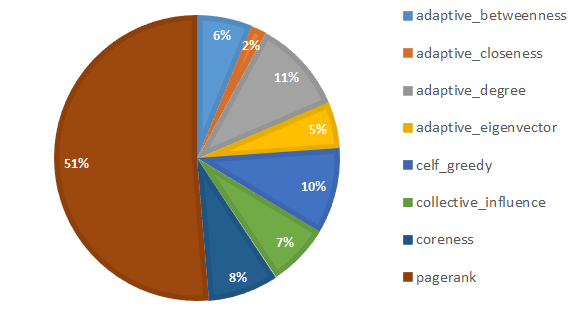
\includegraphics[width=1\textwidth]{inf-summary-budget}
				\caption[IMine performance summary on budget criteria]{Overall summary of percentages of instances in which each method outperformed the other methods in budget criteria. The method with most influence was selected as the best method.}
				\label{fig:inf-summary-budget}
			\end{figure}
			
			\begin{figure}[H]
				\centering
				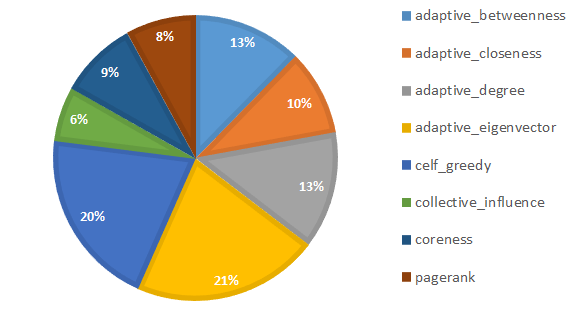
\includegraphics[width=1\textwidth]{inf-summary-influence}
				\caption[IMine performance summary on influence criteria]{Overall summary of percentages of instances in which each method outperformed the other methods in influence criteria. The method which took least time to reach was selected as the best method.}
				\label{fig:inf-summary-influence}
			\end{figure}
	
			\subsubsection{Performance evaluation - efficiency}
			Conventionally, the term efficiency refers to how quickly an action was performed. However, variation in size and type of networks in the data set makes it impractical to use time alone as a measure as the algorithm run time depends highly upon the structural properties; the efficiency is measured as the ratio between the influence and elapsed time, i.e. $\eta=\frac{\sigma}{t}$. The need for this metric can be understood through Figure \ref{fig:inf-summary-min-time}, which shows how frequent a method outperforms others in terms of minimum time. It can be observed that while Coreness has twice as many wins as compared to second best Pagerank algorithm, the percentages in \ref{fig:inf-summary-value-distribution} shows that it is only marginally ahead of Pagerank.
			
			Empirical analysis of results performed on efficiency can be viewed in figure \ref{fig:inf-summary-value-distribution}. The observations solidify the grounds which the IMine framework is built upon. When measuring the efficiency, no single method has significant lead over the others. The top performer, Coreness came out as most efficient in 33\% cases, followed by Pagerank with 27\% win percentage; and finally the Adaptive degree with 24\% winning ratio.
			%In contrast, the Pagerank algorithm had shown significant improvement over other methods in budget trials.
			
			\begin{figure}[H]
				\centering
				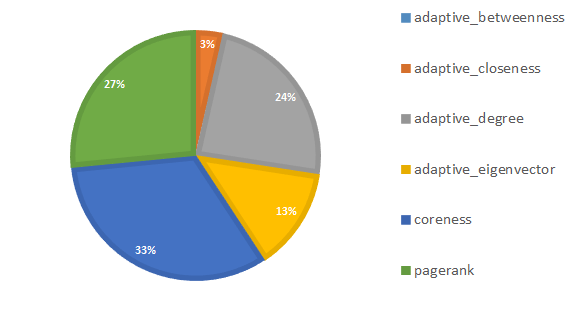
\includegraphics[width=1\textwidth]{inf-summary-max-value}
				\caption[IMine efficiency on influence criteria]{Overall summary of percentages of instances in which each method outperformed the other methods in terms of efficiency for influence criteria. The method with highest $\eta$ is selected as the most efficient method.}
				\label{fig:inf-summary-max-value}
			\end{figure}
	
			\begin{figure}[H]
				\centering
				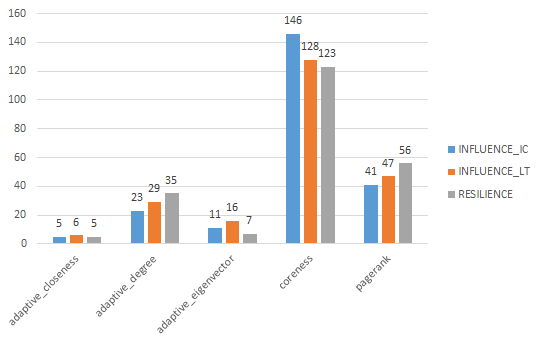
\includegraphics[width=1\textwidth]{inf-summary-min-time}
				\caption[IMine lowest time comparison]{Number of times each method executed in lowest elapsed time as compared to other methods, distributed by test method. The results from both budget and influence trials have been combined.}
				\label{fig:inf-summary-min-time}
			\end{figure}
			
		
			\subsubsection{Hypothesis 1}
			We established that for overall results, the performance of an influence method is not independent on the stoppage criteria, we now observe whether these results stand for all the three influence test methods or not. Figures \ref{fig:inf-summary-budget-distribution} and \ref{fig:inf-summary-influence-distribution} illustrate how the win instances for each method are distributed. 
	
			\begin{figure}[H]
				\centering
				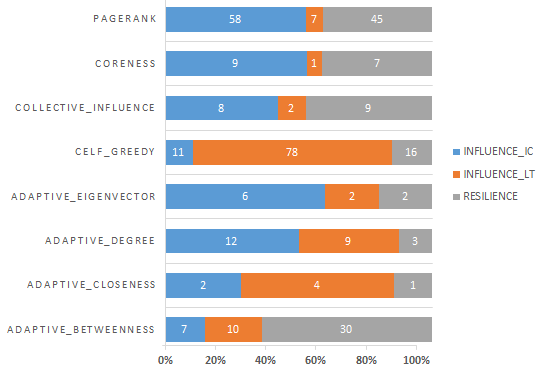
\includegraphics[width=1\textwidth]{inf-summary-budget-distribution}
				\caption[IMine performance on budget criteria on all test methods]{Percentage of number of instances each method outperformed the other methods in budget criteria, distributed by test method. The method with most influence was selected as the best method.}
				\label{fig:inf-summary-budget-distribution}
			\end{figure}
			
			\begin{figure}[H]
				\centering
				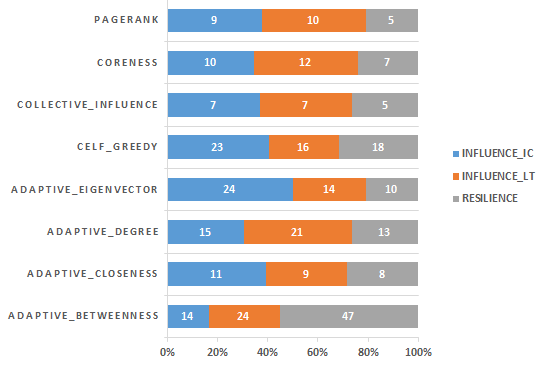
\includegraphics[width=1\textwidth]{inf-summary-influence-distribution}
				\caption[IMine performance on influence criteria on all test methods]{Percentage of number of instances each method outperformed the other methods in influence criteria, distributed by test method. The method with most influence was selected as the best method.}
				\label{fig:inf-summary-influence-distribution}
			\end{figure}		
	
			\begin{figure}[H]
				\centering
				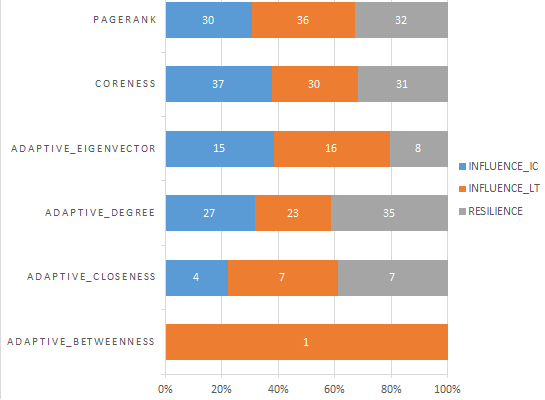
\includegraphics[width=1\textwidth]{inf-summary-value-distribution}
				\caption[IMine efficiency on all test methods]{Percentage of number of instances each method outperformed the other methods in efficiency criteria, distributed by test method. The method with highest efficiency was selected as the best method.}
				\label{fig:inf-summary-value-distribution}
			\end{figure}		
			
			Figures \ref{fig:inf-summary-budget-distribution} and \ref{fig:inf-summary-influence-distribution} are assessed in two stages, first we find the methods which performed well in each test method individually for budget criteria, then these findings are compared with the best performers for influence criteria. If the number of observations where a method that performed well for both criteria consistently is significant, the $H_{1_0}$ will be accepted.
			
			From figure \ref{fig:inf-summary-budget-distribution} we see that for Influence\_IC Pagerank stood as top performer with 58 observations (out of 113), followed by Adaptive Degree with 12 observations; for Influence\_LT, the CELF-greedy outperformed other methods by a wide margin with 78 observations, followed by Adaptive Betweenness with only 10 of such observations; finally, for the Resilience test the Pagerank algorithm again performed better than the rest with 45 observations, followed by Adaptive Betweenness with 30 observations.
			
			In figure \ref{fig:inf-summary-influence-distribution}, a different pattern is observed. For Influence\_IC test, Adaptive Eigenvector method came on top with 24 observations, followed by CELF-greedy only marginally behind with 23 observations. Neither Pagerank, nor Adaptive Degree performed as good as they did for budget criteria; for Influence\_LT, we see Adaptive Betweenness as the best performer with 24 observations, followed closely by Adaptive Degree with 21 wins. Again, the CELF-greedy algorithm which was highly dominant in former test did not perform anywhere close; for Resilience test, Adaptive Betweenness outperformed other methods with 47 observations, followed by CELF-greedy. Pagerank algorithm failed to enlist itself as a top performer.
			
			In a brief manner, for all the three test methods analyzed empirically for both the criteria, out of 12 cases (top 2 performers for all 3 methods on the 2 criteria), only once did we observe a consistent pattern where Adaptive Betweenness was 2nd best for budget and the best for influence criteria. We use Odds Ratio method to evaluate the significance:
			Let $O_{true}$ be the ratio of instances supporting $H_{1_0}$; $O_{false}$ be the ratio of instances against $H_{1_0}$; $N$ be the number of findings; $OR=\frac{O_{false}}{O_{true}}$. Hence, $OR=\frac{11/12}{1/12}=11$. In other words, the $H_{1_0}$ is 11 times unlikely to be true as compared to being false.
			
			We reject $H_{1_0}$ and accept $H_{1_A}$ since in no observation a method ranked similar when changing criteria\footnote{Significance testing is not required since the number of observations supporting the hypothesis is 0}. In the extended analysis, the $H_{1_0}$ is rejected as the Odds Ratio of the number of times an influence method performed consistently well to not performing consistently is 1 to 11.
			
			\subsubsection{Hypothesis 2}
			As stated before, the hypothesis is that there exists no relationship between diffusion and resilience test. We are confirming that both of these tests are indeed different and cannot be used interchangibly.
			
			Table \ref{tab:inf-framework-test-method-comparison} shows how frequently the trials supported $H_{2_1}$ in terms of percentages. The Resilience test is compared with both Influence tests individually as well as combined. The percentages show the ratio of trials in which one or more test methods matched. For example, for graph ArXiv on threshold 0.01, if the most influential method for Resilience test was CELF-greedy, and for Influence\_IC test was Pagerank, and for Influence\_LT was CELF-greedy, then "Resilience = Influence\_LT" and "Resilience = Influence\_IC or Influence\_LT" will both be true. Complete table of each trial can be seen in Appendix \ref{sec:appendix-B-inf-framework}.			
			
			\begin{longtable}[c]{|l|l|l|}
				\hline
				\textbf{}                                            & \textbf{Percentage} & \textbf{Successful Trials} \\ \hline
				\endfirsthead
				%
				\endhead
				%
				\textbf{Resilience = Influence\_IC = Influence\_LT}  & 7.08\%              & 8/113                      \\ \hline
				\textbf{Resilience = Influence\_IC only}             & 42.48\%             & 48/113                     \\ \hline
				\textbf{Resilience = Influence\_LT only}             & 21.24\%             & 24/113                     \\ \hline
				\textbf{Resilience = Influence\_IC or Influence\_LT} & 56.64\%             & 64/113                     \\ \hline
				\caption[Ratio of result matches of resilience test with influence tests]{Percentages of trials in which results of Resilience in terms of the most influential method matched with Influence test results for Budget criteria.}
				\label{tab:inf-framework-test-method-comparison} \\
			\end{longtable}

			The overall results are not supporting the hypothesis. We observe that in only 7.08\% of the trials, the most influential method was found to be same for all the three test methods. On the other extreme, even comparing Resilience test with either of the influence test gave an unimpressive 56.64\%. Let odds ratio $O_{true}$ be the ratio of instances supporting $H_{2_0}$ and $O_{false}$ be the ratio opposing $H_{2_0}$. Therefore the odds ratio $OR=\frac{105/113}{8/113}=13$, i.e. the hypothesis $H_{2_0}$ is unlikely to be false 13 times as compared to being true. The results are insignificant and do not pass the confidence test, we therefore reject $H_{2_0}$ and accept $H_{2_A}$. \\

		These results prove two major points. The first one validates the IMine framework's case by showing that when the stoppage criteria changes, the influence mining methods change their performance. Second point is that Resilience test and Influence tests are not identical; they should not be used interchangeably but rather both tests should be conducted in order to assess the results of any influence mining application.
		
% \subsubsection{Empirical analysis}
% Analyzing individual networks unveiled some interesting observations which we will discuss here. The most prominent and obvious is that not all networks exhibited similar behaviour during influence simulations. Moreover, while we did discuss that there is no single all-rounding best performing heuristic, some of them have shown their dominance over other methods in particular aspects.
		

	\section{IMine Framework Applications}
	\label{sec:inf-framework-applications}
	The previous discussion was around the aggregate results from the IMine framework experiments, which builds the case for the framework. However, the framework itself does not address the key problem of which algorithm to use in what scenario - the universe of types of complex networks and the various techniques to mine influential networks is too vast to experimentally provide a concrete map of which technique is most suitable for what network type, and for which criteria. Nevertheless we discuss the most suitable methods extracted during empirical analysis of the IMine framework validation results. This discussion should provide guidance on which method is likely to be most beneficial against a particular criteria and type of benchmark test.
	
		\subsubsection{Best influence spreader on minimum budget}
		The best method when the budget is minimum in terms of influence spread is CELF-greedy for Budget criteria, leading 37.33\% of the time, followed by Pagerank (28\%), and Adaptive Betweenness for Influence criteria (28.37\%), followed by CELF-greedy (19.86\%). Grouping the results by the test method, Pagerank took the lead in Influence\_IC test with 8.33\% (out of 33\%); CELF-greedy in Influence\_LT with 12.5\% (out of 33\%); Adaptive Betweenness in Resilience with 23.15\% (out of 33\%). Overall, CELF-greedy stands as the best method winning 25.93\% of the trials, closely followed by Adaptive Betweenness winning 23.15\% of the trials. The least favourable methods identified to be Adaptive Closeness and Collective Influence with both having a winning of 6.02\% (detailed results are given in Table \ref{tab:inf-best-min-budget}).
		
		This is the most frequent real-life -- as well as most discussed in research literature -- case in viral marketing, where the aim is to find out $k$ most influential nodes where the value of $k$ is low. A good application here is for tycoons in consumer electronics business. Each year, conferences like CES (Consumer Electronics Show), MWC (Mobile World Congress), and E3 (Electronic Entertainment Expo) take place where international technology manufacturers announce and advertise their upcoming products. In such events, the companies invite enthusiasts and independent journalist in the tech industry such that their reach is maximized.	Due to very high cost associated with each individual target influencer, the relative budget is not very high.
	
		\subsubsection{Best influence spreader on maximum budget}
		The best method when the budget is maximum in terms of influence spread is Pagerank for Budget criteria, leading 39.39\% of the time, followed by CELF-greedy (22.73\%), and Adaptive Betweenness for Influence criteria (20.45\%), followed by CELF-greedy (18.18\%). Grouping the results by the test method, Pagerank took the lead in Influence\_IC test with 8.08\% (out of 33\%); CELF-greedy in Influence\_LT with 9.6\% (out of 33\%); Adaptive Betweenness in Resilience with 12.63\% (out of 33\%). Adaptive betweenness and Pagerank with equal score of 18.69\% tied for best method overall, followed marginally by CELF-greedy with 18.18\%. The least favourable method in this case was Coreness with a score of 6.06\% (detailed results are given in Table \ref{tab:inf-best-max-budget}).
		
		In this scenario, the aim is the same, i.e. to find out $k$ most influential nodes where the value of $k$. However $k$ is relatively high, because the objective is to ensure that the influence is spread to all ends of the network and not only a particular segment. An example for this case is a pharmaceutical company launching a new general-purpose Over the counter (OTC) drug, would increase its marketing budget but ensure that their product reaches most of the pharmacies in the target region.
	
		\subsubsection{Efficient performer in influence on minimum budget}
		Reiterating that efficiency is defined as $\eta=\frac{\sigma}{t}$, where $\sigma$ is the influence measure and $t$ is the time taken. Efficiency is applicable only on Influence criteria since Budget criteria does not stop execution until the desired number of nodes are identified. In our experiments, Coreness appeared atop with 12.06\% (out of 33\%) for Influence\_IC test; for Influence\_LT Coreness and Pagerank both tied with 9.93\% (out of 33\%); Pagerank tied again with Adaptive degree for Resilience test with 10.64\% win ratio. In the aggregate results, Coreness stood as most efficient performer on minimum budget with 29.79\% winning ratio where Pagerank came on 2nd rank with 27.66\% (detailed results are provided in Table \ref{tab:inf-efficient-min-budget}).
		
		This particular case applies to cases like fast fashion industry. An apparel manufacturer has a short time window to sell out its recent articles. As opposed to well-established brands, these businesses are interested in short bursts. Therefore, they will look for an influence method which ensures maximum yield in short time duration and limited marketing budget, no matter if the consumers are within a particular core or cluster of the whole network.
	
		\subsubsection{Efficient performer in influence on maximum budget}
		In this case, Coreness lead again for maximum budget with 10.61\% (out of 33\%) for Influence\_IC test; for Influence\_LT Pagerank came atop with 10.61\% (out of 33\%); for Resilience test, Pagerank won with 10.61\%; in Resilience test Coreness, Adaptive degree and Pagerank came very close to each other with 9.85\%, 9.0\% and 9.0\% respectively. Overall, Pagerank was identified as most efficient performer on maximum budget with 29.55\% winning ratio where Pagerank came next with 28.79\%, only marginally behind (detailed results are given in Table \ref{tab:inf-efficient-max-budget}).
		
		As an example, imagine a company like Apple Inc. which produces high-quality electronic goods. In order to sell a back-to-school product like a student grade laptop, they would be interested not only in penetrating the market, but rather dominating it. Therefore when targeting students in a University, they'll market to each college and department with a rigorous campaign (high budget) in as little time as possible to avoid competition.
	
		\subsubsection{First to reach desired influence on minimum budget}
		Coreness outperformed all other methods in this scenario spectacularly, scoring 19.15\% (out of 33\%) in Influence\_IC and 14.89\% (out of 33\%) in Influence\_LT tests; it only lost in Resilience test to Adaptive degree and Pagerank with both scoring 10.64\%. Average results on all tests crowned Coreness with 41.84\% win percentage where the next best was Adaptive degree with 23.40\%, which is significantly below Coreness (detailed results are given in Table \ref{tab:inf-fast-min-budget}).
		
		This case is more applicable to advertisement than marketing where the aim is not the yield but to generate awareness \textit{before} the actual product is launched. A politician running his campaign before elections is a good example here, who may be interested in disruptive marketing by targeting a few influential figures in public gatherings. Since there is unlikely to have a budget to reach all communities, and considering that the opposing parties are also simultaneously campaigning, the candidate will ensure that his message reaches to the voters in a specific proximity quickly.	
	
		\subsubsection{First to reach desired influence on maximum budget}
		The results in this case exhibit an interesting phenomenon, that the increase in budget turned favour towards Pagerank. In the Influence\_IC test, Coreness still maintained its lead over other methods with 13.64\% results in favour, however for Influence\_LT and Resilience tests, Pagerank scored highest with 10.61\% and 12.12\% win percentage respectively. In overall results, Coreness although remained best performer with an average win percentage of 31.06\%, Pagerank closely followed with 29.55\% (detailed results are given in Table \ref{tab:inf-fast-max-budget}).
	
		A suitable application is virus propagation in a large computer network. The attacker is not constrained by budget, but rather time before the compromise is detected. Therefore an algorithm such as Pagerank can be used to identify which particular nodes in the network are likely to disrupt a wide range of network in the shortest time.
		

	\section{Summary}
	Current state-of-art methodologies have two limitations. The convergence criteria, which stops the influence mining process is fixed to the number of nodes, i.e. budget; real-life applications do not work soleley on this criteria. Secondly, the influence quantifier has been fixed to either influence or resilience test. We build a conjecture based on three experiments that a framework is needed for influence mining. In response, we unveil IMine, a framework which allows an application to adopt certain influence method, define custom stoppage criteria, and choose a method to quantify the influence itself by reforming the original resilience algorithm.
	
	The IMine is put to the test on 22 networks with respect to accuracy and efficiency. To the best of our knowledge, this is the most comprehensive test performed to evaluate any particular influence mining strategy. Two criteria were passed to test against eight heuristics for five values of criteria on same computer. The results prove that both the hypotheses were rejected. The chapter concluded with a few examples of where the IMine framework can be applied in real life.


	\chapter{Conclusion and Future Work}
\label{chp:conclusion}

This research encompasses a few aspects of the vast field of graph analysis and mining. Specifically we focus on the identification and discovery of most influential nodes, which have the capability to trigger a ripple effect of any event (news, disease spread, political movement, viral content, etc.) in a real-world connected system.

The problem of identifying influential nodes often termed as influence maximization is a complex problem, and the closest polynomial-time solution is Hill-climbing greedy-based approach which exploits the monotone property and the sub-modular property of the problem. The manuscript then moves to perform three experiments to practically evaluate the problem and propose interim solutions to further the state-of-art.

	\section{Conclusion}
	The first experiment scrutinized a popular phenomenon that is various methods and heuristics used to discover influential nodes produce  inconsistent results on different types of networks. The experiments concluded that although these complex networks (both real and synthetic) show some structural similarities, there are stark differences that result in the inconsistent behavior of various methods and heuristics. For example: a complex network can have dense communities and another complex network can be a stark contrast with low community structure; small-world networks have high clustering coefficients; on average betweenness centrality is better among centrality-based methods for influence maximization problem. Nevertheless, the conclusion derived was that it is in fact not the structure of the network, but rather the method of selecting seed nodes, which affects the diffusion process on different networks.
	
	Second experiment evaluated two snapshots of a real-world network of global business ties from year 2010 and 2013, to analyze the diversity, strength and centrality of cities. In this experiment, the resilience test was used to identify the most influential cities. Our results gave not only new insights about the role of cities in the global economic network, but also validated resilience test with ground truth. For example, Paris, London and New York turned out to be most important cities. Lastly and most importantly, we witnessed that a state-of-art method performed below three classical methods which reinstated that in real scenarios, there is no guarantee that a particular heuristic will surely be effective.
	
	From the experiments, we established three facts:
	
	\begin{enumerate}
		\item In complex networks, each seed selection method has different effect on the influence maximization problem.
		
		\item There is no algorithm which is accurate, scalable, and has low time and space requirements for the influence maximization problem.
		
		\item Influence test is not the only test to benchmark seed nodes. Resilience test is also widely used test to evaluate performance of an influence function.
		
	\end{enumerate}    
	
	In spite of there being lack of a single method which is highly accurate, scalable, and has low memory requirements research community proposed numerous different approaches, each with their pros and cons. We took a novel approach of applying machine learning techniques for influence mining by training on 367 complex networks with variation in structural attributes. The experiment not only used public networks frequently used in literature, but also two newly extracted networks from online social networks, and 120 synthetically generated networks. The results suggested that eXtreme Gradient Boosting model outperformed both classic and state-of-art heuristics in identifying most influential nodes. However, this approach had two key problems:
	
	\begin{enumerate}
		\item the model would only work on the sizes of networks included in training set, and perform poorly on a network of size significantly different than those used during training.
		
		\item in order to rigorously train the models, we first needed to provide the set of optimal seed nodes as target nodes. This is because eXtreme Gradient Boosting is a supervised machine learning method. Finding an optimal set of seed nodes is possible even on mid-sized networks, and even the greedy method would become impractical on large-scale networks.
	\end{enumerate}
	
	The final part of the research proposes a response to these dimensions - the IMine Framework. This framework enables customization of the implementation of IM problem. Instead of assuming that the budget, i.e. the number of seed nodes to extract as the only criteria to stop the IM process, IMine accepts the stoppage criteria function and its respective threshold as a parameter to the IM algorithm. Thus, providing a horizontal platform to lay the custom implementations. With IMine, the implementer is not forced to adopt one algorithm for influence mining, but change the algorithm based on the stoppage criteria. Therefore, for a use case where the time is primary constraint, the influence method to be passed should be the one which is most efficient, rather than most accurate. There is no realistic limit to how many criteria there can be, therefore an implementer can try and test several heuristics using IMine and choose the one closest to the use case.
	
	\section{Future work}
	The work presented in this thesis is ripe for researchers focusing in this area. First, the empirical study can be expanded to more real networks and state-of-art algorithms.
	
	The machine learning experiment was not comprehensive, and merely provides a proof of concept. It will be worthwhile to investigate whether with the help of deep learning on Big data, the machine learning solution converges to a particular network trait which solves the problem for 99\% of the time. Moreover, the time complexity to train the model itself is to be considered; the experiment presented assumes that the learning data will have known ground truth, either by using domain knowledge or finding out the optimal seed set. This is obviously impractical for large scale experiments. Furthermore, the technique seems to remain infaffective for smaller networks, while it can be argued that there is an abundance of methods which perform very well on small networks out of the box, it would be fruitful to train a model which will perform better on small networks of a wide variety so as to achieve generalization. The work presented focuses either on Time complexity or Accuracy, the study steered clear of an important aspect, i.e. space complexity. Therefore in that manner, there is an induced bias towards the heuristics and methods which are either efficient, or accurate. The same series of experiments can be modified to include memory consumption data for new insights. An important constraint which the IMine framework suffers from, is that most of the state-of-art algorithms require reconstruction with added stoppage criteria, since they were not originally designed for objectives other than budget. While we did modify Collective Influence, Pagerank and CELF++, some notable algorithms like TIM, SIMPATH, IMM, EasyIM are a must because of their unique selling points and strengths. Among the most prominent enhancements that can be made is learning from the feedback from raw data collected as results in the final experiment and developing a recommendation system, which suggests the most appropriate heuristic for a given criteria and threshold. IMIne is a fitting framework to setup a very large scale experiment on these lines.
	
	In order to aid the researchers willing to build on the IMine framework, the complete source code and all the data sets are made publicly available at \cite{hussain2020}.

	
	% ********************************** References ******************************
	\begin{spacing}{0.8}
		
		% To use the conventional natbib style referencing
		% Bibliography style previews: http://nodonn.tipido.net/bibstyle.php
		% Reference styles: http://sites.stat.psu.edu/~surajit/present/bib.htm
		
		%\bibliographystyle{apalike}
		\bibliographystyle{unsrt} % Use for unsorted references  
        
		%\bibliographystyle{plainnat} % use this to have URLs listed in References
        
		\cleardoublepage
		\begin{small}
		\bibliography{references} % Path to your References.bib file
		\end{small}
	
		% If you would like to use BibLaTeX for your references, pass `custombib' as
		% an option in the document class. The location of 'reference.bib' should be
		% specified in the preamble.tex file in the custombib section.
		% Comment out the lines related to natbib above and uncomment the following line.
		
		%\printbibliography[heading=bibintoc, title={References}]
		
		
	\end{spacing}
	
	% ********************************** Appendices ********************************
	
	\begin{appendices} % Using appendices environment for more functionality
		
		%!TEX root = ../glossary.tex
% ******************************* Thesis Appendix A: Glossaries ****************************

\chapter{Glossary}

% Please add the following required packages to your document preamble:
% \usepackage{booktabs}
% \usepackage{longtable}
% Note: It may be necessary to compile the document several times to get a multi-page table to line up properly

In ascending order; abbreviations are followed by their respective acronyms in parenthesis.

Action: An activity performed by a user in a network.

Adjacency Matrix: $n\times n$ matrix of nodes showing edges between them.

APL (Average Path Length): Average number of edges between shortest paths among nodes, given as $l\dfrac{1}{n(n-1)}\sum_{i,j}d_{i,j}$ where $i,j$ is any pair of nodes, $l$ is the number of nodes in the path between $i$ and $j$ and $n$ is total number of nodes in the network.

Assortativity: Pearson correlation coefficient of nodes at any side of an edge. Ranging between -1 and 1, negative value means that the high degree nodes tend to connect with low degree nodes, positive value means that the nodes connect with respect to degree similarity.

Average Degree: Average number of edges for each node.

Average Distance: Average number of edges between any pair of nodes in a network.

Betweenness Centrality: Number of shortest paths between all pairs of nodes passing through a nodes.

Centrality: A measure of central tendency of a node in a network.

CC (Clustering Coefficient): Ratio of number of Triads connected to a node to possible number of Triads.

CC (global): Global CC or Clique-ness of a network given as $C_{global}=\dfrac{3\times |triads|}{|possible triads}$.

CES: Consumer Electronics Show is organized by the Consumer Technology Association annually for electronics traders.

CI (Collective Influence): Heuristic for seed selection, scalable on large networks.

Clique: Completely connected network, i.e. every node has an edge with every other node (number of triads in a clique are $3^{n-3}$).

Closeness Centrality: Number of steps required to reach every node in a network from a node. Calculated as $\dfrac{1}{\sum_{i\in V}d_{u,i}}$, where $d_{u,i}$ is the distance from node $u$ to all other nodes $i\in V$.

Connected Network: A network in which each node can reach any other node.

Coreness: Measure that defines how many neighbours a node has. A node is in core $k$ if its degree is k, not $k-1$ or $k+1$.

DAC (Directed Acyclic Graph): A directed graph with no directed cycles.

Degree: Number of edges of a node.

Degree of Influence: Percentage of influence of a node on its neighbours.

Density: Ratio between existing network edges and all possible edges among nodes.

Diameter: Number of edges in longest path that exists from two most distinct nodes.

Diffusion: Spread of an event or action in a network.

E3: Electronic Entertainment Expo is an international video game industry event held annually by The Entertainment Software Association (ESA).

Edge Betweenness: Number of shortest paths on which an edge lies.

Highest Degree: Maximum number of connections of any individual node in a network.
	
IC (Independent Cascade): Diffusion model, which assumes that an active node can attempt to activate another inactive node in its neighbourhood, independent of past actions and other active nodes.

In-Degree: Number of edges directing towards a node in a directed network.

Influence: Tendency of a node to trigger another node to repeat an action performed initially by itself in a network.

IM (Influence Maximization): Phenomenon of maximizing influence of a set of nodes or actions on a network.

LT (Linear Threshold): Diffusion model, which assumes that an inactive node can become active only when a certain activation threshold is met.

MWC: Mobile World Congress is an annual conference specific to mobile phone industry. It is organized by GSMA each year.

Neighbour: A node adjacent (directly connected) to a node.

Network: A graph consisting of nodes and edges between them.

Network Diameter: \textit{see Diameter}.

Normalization: Method to normalize data.

Out-Degree: Number of edges directing from a node to others in a network.

Path: Set of edges from one node to another.

SIR (Susceptible-Infected-Recovered): an epidemiology model in which an individual susceptible to a disease becomes infected with some probability, then Recovered with some recovery probability, then is not infected again.

SIS (Susceptible-Infected-Susceptible): an epidemiology model in which an individual susceptible to a disease becomes infected with some probability, then becomes Susceptible again.

Triad/Triangle: Set of 3 interconnected nodes in a network.

WC (Weighted Cascade): Diffusion model, which assumes that an active node can attempt to activate another node with some probability (weight) learned from past progressions.

        
        % Supplementary Tables
        %!TEX root = ../appendix-B.tex
% ******************************* Thesis Appendix B: Tables ****************************

\chapter{Tables}
\label{chp:tables}

\section{Diversity, Strength and Centrality in city networks}
\label{sec:appendix-B-city-networks}

\begin{table}[h]
	\centering
	\caption{List of Top 25 Cities with Increased Diversity}
	\begin{scriptsize}
	\begin{tabular}{|l|c|c|c|}
	\hline \textbf{Rank} & \textbf{City} & \textbf{Country} & \textbf{Region}  			\\   
	\hline 
	 1. & Baltimore         & United States of America 			& North America 		\\	
	 2. & Jersey      		& United Kingdom 					& Western Europe  		\\	
	 3. & Mannheim 			& Germany 							& Western Europe  		\\	
	 4. & Hanover 			& Germany 							& Western Europe 		\\	
	 5. & Geneva 			& Switzerland 						& Western Europe 		\\	
	 6. & Milan 			& Italy 							& Western Europe 		\\	
	 7. & Nicosia 			& Cyprus 							& Eastern Europe 		\\	
	 8. & Dubai 			& United Arab Emirates 				& Western Asia			\\	
	 9. & Akrotiri 			& Cyprus 							& Eastern Europe		\\	
	 10. & Antwerp 			& Belgium 							& Western Europe		\\	
	 11. & Bucharest 		& Romania 							& Eastern Europe		\\	
	 12. & San Francisco 	& United States of America 			& North America			\\	
	 13. & Beijing 			& China 							& Eastern Asia  		\\	
	 14. & Abu Dhabi	 	& United Arab Emirates 				& Western Asia			\\ 
	 15. & Lagos  			& Nigeria 							& Western Africa		\\ 				
	 16. & Phoenix 			& United States of America  		& North America    		\\ 
	 17. & Zurich 			& Switzerland 						& Western Europe  		\\
	 18. & Maastricht 		& Netherlands  						& Western Europe   		\\
	 19. & Tampa 			& United States of America  		& North America   		\\
	 20. & Shanghai 		& China 							& Eastern Asia  		\\
	 21. & Sydney 			& Australia 						& Australia/Oceania		\\
	 22. & London 			& United Kingdom  					& Western Europe 		\\
	 23. & Kansas City 		& United States of America  		& North America 		\\
	 24. & Cleveland 		& United States of America  		& North America   		\\
	 25. & Yokohama 		& Japan  							& Eastern Asia  		\\
	\hline
	\end{tabular} 
	\end{scriptsize}
	\label{tab:appendix-B-increasing}
\end{table}


\begin{table}[h]
	\centering
	\caption{List of Top 25 Cities with Decreased Diversity}
	\begin{scriptsize}
	\begin{tabular}{|l|c|c|c|}
	\hline \textbf{Rank} & \textbf{City} & \textbf{Country} & \textbf{Region} 			 \\   
	\hline 
	 1. & Stockholm         & Sweden 							& Western Europe  		\\	
	 2. & Goteborg      	& Sweden 							& Western Europe  		\\	
	 3. & Rome 				& Italy 							& Western Europe  		\\	
	 4. & Copenhagen 		& Denmark 							& Western Europe 		\\	
	 5. & Charlotte 		& United States of America			& North America			\\	
	 6. & Sonderborg 		& Denmark 							& Western Europe 		\\	
	 7. & Cincinnati 		& United States of America			& North America			\\	
	 8. & Aarhus 			& Denmark 							& Western Europe 		\\	
	 9. & Munster 			& Germany 							& Western Europe		\\	
	 10. & Frankfurt 		& Germany 							& Western Europe		\\	
	 11. & Clermont Ferrand & France 							& Western Europe		\\	
	 12. & Dundee			& United Kingdom		 			& Western Europe		\\	
	 13. & Shannon 			& Ireland 							& Western Europe  		\\	
	 14. & Torino	 		& Italy				 				& Western Europe		\\ 
	 15. & Novosibirsk		& Russia 							& Eastern Europe		\\ 				
	 16. & Angouleme		& France 							& Western Europe		\\	
	 17. & Kuwait 			& Kuwait	 						& Western Asia	  		\\
	 18. & Omaha 			& United States of America  		& North America   		\\
	 19. & Porto 			& Portugal							& Western Europe  		\\
	 20. & Friedrichshafen 	& Germany 							& Western Europe  		\\
	 21. & Siena 			& Italy 							& Western Europe		\\
	 22. & Perm 			& Russia		 					& Eastern Europe 		\\
	 23. & Akron Canton		& United States of America  		& North America 		\\
	 24. & Milwaukee 		& United States of America  		& North America   		\\
	 25. & Vitoria 			& Spain  							& Western Asia  		\\
	\hline
	\end{tabular} 
	\end{scriptsize}
	\label{tab:appendix-B-diversity-decreasing}
\end{table}


\begin{table}[h]
	\centering
	\caption{List of Top 25 Cities with Increased Strength}
	\begin{scriptsize}
	\begin{tabular}{|l|c|c|c|}
	\hline \textbf{Rank} & \textbf{City} & \textbf{Country} & \textbf{Region} 			\\   
	\hline 
	 1. & Philadelphia      & United States of America 			& North America 		\\	
	 2. & Milan      		& Italy			 					& Western Europe  		\\	
	 3. & Chicago 			& United States of America 			& North America 		\\	
	 4. & Baltimore 		& United States of America 			& North America 		\\	
	 5. & Beijing 			& China 							& Eastern Asia	 		\\	
	 6. & San Francisco 	& United States of America 			& North America 		\\	
	 7. & Tokyo 			& Japan 							& Eastern Asia	 		\\		
	 8. & Zurich 			& Switzerland		 				& Western Europe		\\	
	 9. & Boston 			& United States of America 			& North America 		\\	
	 10. & Lille 			& France 							& Western Europe		\\	
	 11. & Sydney 			& Australia 						& Australia/Oceania		\\	
	 12. & Los Angeles 		& United States of America 			& North America			\\	
	 13. & Singapore 		& Singapore							& Eastern Asia  		\\	
	 14. & Shanghai	 		& China				 				& Eastern Asia			\\ 
	 15. & Luxembourg  		& Luxembourg 						& Western Europe		\\ 				
	 16. & Houston 			& United States of America  		& North America    		\\ 
	 17. & Grand Cayman 	& Cayman Islands 					& Caribbean		  		\\
	 18. & Mannheim 		& Germany	  						& Western Europe   		\\
	 19. & Detroit 			& United States of America  		& North America   		\\
	 20. & Geneva	 		& Switzerland		 				& Western Europe		\\	
	 21. & Sao Paulo 		& Brazil	 						& South America			\\
	 22. & Denver 			& United States of America  		& North America 		\\
	 23. & Toronto	 		& Canada					  		& North America 		\\
	 24. & Bucharest 		& Romania					  		& Eastern Europe   		\\
	 25. & Bologna 			& Italy  							& Western Europe   		\\
	\hline
	\end{tabular} 
	\end{scriptsize}
	\label{tab:appendix-B-strength-increasing}
\end{table}


\begin{table}[h]
	\centering
	\caption{List of Top 25 Cities with Decreased Strength}
	\begin{scriptsize}
	\begin{tabular}{|l|c|c|c|}
	\hline \textbf{Rank} & \textbf{City} & \textbf{Country} & \textbf{Region}  \\   
	\hline 
	 1. & Moscou 		    & Russia				 			& Eastern Europe 		\\	
	 2. & Frankfurt    		& Germany		 					& Western Europe  		\\	
	 3. & Stockholm 		& Sweden				 			& Western Europe 		\\	
	 4. & London	 		& United Kingdom 					& Western Europe 		\\	
	 5. & Charlotte 		& United States of America 			& North America 		\\	
	 6. & Dusseldorf	 	& Germany				 			& Western Europe 		\\	 			
	 7. & Munich			& Germany				 			& Western Europe 		\\	 			
	 8. & Copenhagen 		& Denmark			 				& Western Europe		\\	
	 9. & Cologne 			& Germany				 			& Western Europe		\\	
	 10. & Milwaukee		& United States of America 			& North America			\\	
	 11. & Birmingham 		& United Kingdom					& Western Europe		\\	
	 12. & Saint Petersbourg& Russia			 				& Eastern Europe		\\	
	 13. & Leeds 			& United Kingdom					& Western Europe		\\	
	 14. & Barcelona	 	& Spain				 				& Western Europe		\\	
	 15. & Hong Kong  		& Hong Kong 						& Eastern Asia			\\ 				
	 16. & Manchester 		& United Kingdom					& Western Europe		\\	
	 17. & Goteborg 		& Sweden 							& Western Europe		\\	
	 18. & Osaka 			& Japan	  							& Eastern Asia   		\\
	 19. & Rotterdam		& Netherlands 				 		& Western Europe		\\	
	 20. & Samara	 		& Russia			 				& Eastern Europe		\\	
	 21. & Nuremberg 		& Germany	 						& Western Europe		\\	
	 22. & Glasgow 			& United Kingdom			  		& Western Europe 		\\
	 23. & Southhampton		& United Kingdom			  		& Western Europe 		\\
	 24. & Bermuda Kindley	& Bermuda					  		& North America   		\\
	 25. & Novosibirsk 		& Russia  							& Eastern Europe   		\\
	\hline
	\end{tabular} 
	\end{scriptsize}
	\label{tab:appendix-B-strength-decreasing}
\end{table}


\begin{table}[ht]
	\centering
	\caption{List of Top 25 Cities with Increased Centrality}
	\begin{scriptsize}
	\begin{tabular}{|l|c|c|c|}
	\hline \textbf{Rank} & \textbf{City} & \textbf{Country} & \textbf{Region}  			\\   
	\hline 
	 1. & Akrotiri      	& Cyprus 							& Eastern Europe 		\\	
	 2. & Nizhniy Novgorod  & Russia		 					& Eastern Europe  		\\	
	 3. & Dubai 			& United Arab Emirates				& Western Asia	 		\\	
	 4. & Ekaterinburg 		& Russia		 					& Eastern Europe  		\\	
	 5. & Guernsey 			& United Kingdom 					& Western Europe 		\\	
	 6. & Gdansk			& Poland				 			& Eastern Europe  		\\	
	 7. & Salzburg 			& Austria 							& Western Europe 		\\		
	 8. & Tampere 			& Finland			 				& Western Europe		\\	
	 9. & Tirana 			& Albania				 			& Eastern Europe 		\\	
	 10. & Taegu 			& Republic of Korea					& Eastern Asia			\\	
	 11. & Fuzhou 			& China 							& Eastern Asia			\\	
	 12. & Tianjin	 		& China					 			& Eastern Asia			\\	
	 13. & Jersey	 		& United Kingdom					& Western Europe  		\\	
	 14. & Vilnius	 		& Lithuania			 				& Eastern Europe		\\ 
	 15. & Ciudad Juarez 	& Mexico	 						& Central America		\\ 				
	 16. & Baltimore		& United States of America  		& North America    		\\ 
	 17. & Barbados		 	& Barbados		 					& Caribbean		  		\\
	 18. & Chengdu 			& China	  							& Eastern Asia   		\\
	 19. & Reims 			& France 							& Western Europe   		\\
	 20. & Penang	 		& Malaysia			 				& Eastern Asia			\\	
	 21. & Pusan	 		& Republic of Korea					& Eastern Asia			\\	
	 22. & Abu Dhabi		& United Arab Emirates		  		& Western Asia	 		\\
	 23. & Xiamen	 		& China						  		& Eastern Asia	 		\\
	 24. & Cairo	 		& Egypt						  		& North Africa   		\\
	 25. & Curitiba			& Brazil  							& South America   		\\
	\hline
	\end{tabular} 
	\end{scriptsize}
	\label{tab:appendix-B-centrality-increasing}
\end{table}


\begin{table}[ht]
	\centering
	\caption{List of Top 25 Cities with Decreased Centrality}
	\begin{scriptsize}
	\begin{tabular}{|l|c|c|c|}
	\hline \textbf{Rank} & \textbf{City} & \textbf{Country} & \textbf{Region}  			\\   
	\hline 
	 1. & Goteborg 		    & Sweden				 			& Western Europe 		\\	
	 2. & Sonderborg   		& Denmark		 					& Western Europe  		\\	
	 3. & Kaliningrad 		& Russia				 			& Eastern Europe 		\\	
	 4. & Chelyabinsk 		& Russia 							& Eastern Europe 		\\	
	 5. & Vitoria	 		& Spain					 			& Western Europe 		\\	
	 6. & Gloucester Cheltenham 	& United Kingdom 			& Western Europe 		\\	 			
	 7. & Oulu				& Finland				 			& Western Europe 		\\	 			
	 8. & Bergen 			& Norway			 				& Western Europe		\\	
	 9. & Friedrichshafen 	& Germany				 			& Western Europe		\\	
	 10. & Graz				& Austria 							& Western Europe		\\	
	 11. & Shannon	 		& Ireland							& Western Europe		\\	
	 12. & Jinan 			& China				 				& Eastern Asia			\\	
	 13. & Winnipeg 		& Canada							& North America			\\	
	 14. & Matsumoto	 	& Japan				 				& Eastern Asia			\\	
	 15. & Zhuhai	  		& China		 						& Eastern Asia			\\ 				
	 16. & Ostend 			& Belgium							& Western Europe		\\	
	 17. & Clermont Ferrand	& France 							& Western Europe		\\	
	 18. & Tulsa 			& United States of America			& North America   		\\
	 19. & Salt Lake City	& United States of America			& North America   		\\
	 20. & Parma	 		& Italy				 				& Western Europe		\\	
	 21. & Durban	 		& South Africa 						& Southern Africa		\\	
	 22. & Kuwait 			& Kuwait			  				& Western Asia	 		\\
	 23. & Erfurt			& Germany					  		& Western Europe 		\\
	 24. & Annecy			& France					  		& Western Europe   		\\
	 25. & Murcia	 		& Spain  							& Western Europe   		\\
	\hline
	\end{tabular} 
	\end{scriptsize}
	\label{tab:appendix-B-centrality-decreasing}
\end{table}


\section{The Influence Mining Framework}
\label{sec:appendix-B-inf-framework}

\begin{longtable}[c]{|l|l|l|l|l|}
	\hline
	\textbf{Method} & \textbf{Influence\_IC} & \textbf{Influence\_LT} & \textbf{Resilience} & \textbf{Total} \\ \hline
	\endfirsthead
	%
	\endhead
	%
	\multicolumn{5}{|l|}{\textbf{On BUDGET criteria}}             \\ \hline
	adaptive\_betweenness & 1.33\%  & 5.33\%  & 6.67\%  & 13.33\% \\ \hline
	adaptive\_closeness   & 1.33\%  & 0.00\%  & 1.33\%  & 2.67\%  \\ \hline
	adaptive\_degree      & 2.67\%  & 2.67\%  & 0.00\%  & 5.33\%  \\ \hline
	adaptive\_eigenvector & 1.33\%  & 0.00\%  & 1.33\%  & 2.67\%  \\ \hline
	celf\_greedy          & 4.00\%  & 22.67\% & 10.67\% & 37.33\% \\ \hline
	collective\_influence & 2.67\%  & 2.67\%  & 2.67\%  & 8.00\%  \\ \hline
	coreness              & 0.00\%  & 0.00\%  & 2.67\%  & 2.67\%  \\ \hline
	pagerank              & 20.00\% & 0.00\%  & 8.00\%  & 28.00\% \\ \hline
	\multicolumn{5}{|l|}{\textbf{On INFLUENCE criteria}}          \\ \hline
	adaptive\_betweenness & 4.96\%  & 9.22\%  & 14.18\% & 28.37\% \\ \hline
	adaptive\_closeness   & 4.96\%  & 2.84\%  & 0.00\%  & 7.80\%  \\ \hline
	adaptive\_degree      & 4.26\%  & 4.96\%  & 3.55\%  & 12.77\% \\ \hline
	adaptive\_eigenvector & 4.96\%  & 3.55\%  & 2.84\%  & 11.35\% \\ \hline
	celf\_greedy          & 4.96\%  & 7.09\%  & 7.80\%  & 19.86\% \\ \hline
	collective\_influence & 2.13\%  & 0.71\%  & 2.13\%  & 4.96\%  \\ \hline
	coreness              & 4.96\%  & 3.55\%  & 2.13\%  & 10.64\% \\ \hline
	pagerank              & 2.13\%  & 1.42\%  & 0.71\%  & 4.26\%  \\ \hline
	\caption[IMine accuracy of influence methods on low budget]{Performance of influence methods on all graphs on low-budget (0.125 and under)}
	\label{tab:inf-best-min-budget}
\end{longtable}

\begin{longtable}[c]{|l|l|l|l|l|}
	\hline
	\textbf{Method} & \textbf{Influence\_IC} & \textbf{Influence\_LT} & \textbf{Resilience} & \textbf{Total} \\ \hline
	\endfirsthead
	%
	\endhead
	%
	\multicolumn{5}{|l|}{\textbf{On BUDGET criteria}}             \\ \hline
	adaptive\_betweenness & 1.52\%  & 3.03\%  & 10.61\% & 15.15\% \\ \hline
	adaptive\_closeness   & 0.00\%  & 1.52\%  & 0.00\%  & 1.52\%  \\ \hline
	adaptive\_degree      & 4.55\%  & 3.03\%  & 1.52\%  & 9.09\%  \\ \hline
	adaptive\_eigenvector & 3.03\%  & 1.52\%  & 0.00\%  & 4.55\%  \\ \hline
	celf\_greedy          & 1.52\%  & 19.70\% & 1.52\%  & 22.73\% \\ \hline
	collective\_influence & 1.52\%  & 0.00\%  & 1.52\%  & 3.03\%  \\ \hline
	coreness              & 3.03\%  & 1.52\%  & 0.00\%  & 4.55\%  \\ \hline
	pagerank              & 18.18\% & 3.03\%  & 18.18\% & 39.39\% \\ \hline
	\multicolumn{5}{|l|}{\textbf{On INFLUENCE criteria}}          \\ \hline
	adaptive\_betweenness & 2.27\%  & 4.55\%  & 13.64\% & 20.45\% \\ \hline
	adaptive\_closeness   & 3.03\%  & 2.27\%  & 3.79\%  & 9.09\%  \\ \hline
	adaptive\_degree      & 3.03\%  & 6.06\%  & 3.79\%  & 12.88\% \\ \hline
	adaptive\_eigenvector & 9.09\%  & 5.30\%  & 3.79\%  & 18.18\% \\ \hline
	celf\_greedy          & 9.09\%  & 4.55\%  & 2.27\%  & 15.91\% \\ \hline
	collective\_influence & 3.03\%  & 3.79\%  & 1.52\%  & 8.33\%  \\ \hline
	coreness              & 0.76\%  & 3.79\%  & 2.27\%  & 6.82\%  \\ \hline
	pagerank              & 3.03\%  & 3.03\%  & 2.27\%  & 8.33\%  \\ \hline
	\caption[IMine accuracy of influence methods on high budget]{Performance of influence methods on all graphs on high-budget (0.05 and over)}
	\label{tab:inf-best-max-budget}
\end{longtable}

\begin{longtable}[c]{|l|l|l|l|l|}
	\hline
	\textbf{Method} & \textbf{Influence\_IC} & \textbf{Influence\_LT} & \textbf{Resilience} & \textbf{Total} \\ \hline
	\endfirsthead
	%
	\endhead
	%
	\multicolumn{5}{|l|}{\textbf{On INFLUENCE criteria}}         \\ \hline
	adaptive\_betweenness & 0.00\%  & 0.00\%  & 0.00\%  & 0.00\%  \\ \hline
	adaptive\_closeness   & 0.71\%  & 2.13\%  & 1.42\%  & 4.26\%  \\ \hline
	adaptive\_degree      & 9.93\%  & 5.67\%  & 10.64\% & 26.24\% \\ \hline
	adaptive\_eigenvector & 3.55\%  & 5.67\%  & 2.84\%  & 12.06\% \\ \hline
	coreness              & 12.06\% & 9.93\%  & 7.80\%  & 29.79\% \\ \hline
	pagerank              & 7.09\%  & 9.93\%  & 10.64\% & 27.66\% \\ \hline
	celf\_greedy          & 0.00\%  & 0.00\%  & 0.00\%  & 0.00\%  \\ \hline
	collective\_influence & 0.00\%  & 0.00\%  & 0.00\%  & 0.00\%  \\ \hline
	\caption[IMine efficiency of influence methods on low budget]{Efficiency of influence methods on all graphs on low-budget (0.01 and under)}
	\label{tab:inf-efficient-min-budget}
\end{longtable}

\begin{longtable}[c]{|l|l|l|l|l|}
	\hline
	\textbf{Method} & \textbf{Influence\_IC} & \textbf{Influence\_LT} & \textbf{Resilience} & \textbf{Total} \\ \hline
	\endfirsthead
	%
	\endhead
	%
	\multicolumn{5}{|l|}{\textbf{On INFLUENCE criteria}}         \\ \hline
	adaptive\_betweenness & 0.00\%  & 0.76\%  & 0.00\% & 0.76\%  \\ \hline
	adaptive\_closeness   & 1.52\%  & 2.27\%  & 3.03\% & 6.82\%  \\ \hline
	adaptive\_degree      & 5.30\%  & 8.33\%  & 9.09\% & 22.73\% \\ \hline
	adaptive\_eigenvector & 6.06\%  & 3.03\%  & 2.27\% & 11.36\% \\ \hline
	coreness              & 10.61\% & 8.33\%  & 9.85\% & 28.79\% \\ \hline
	pagerank              & 9.85\%  & 10.61\% & 9.09\% & 29.55\% \\ \hline
	celf\_greedy          & 0.00\%  & 0.00\%  & 0.00\% & 0.00\%  \\ \hline
	collective\_influence & 0.00\%  & 0.00\%  & 0.00\% & 0.00\%  \\ \hline
	\caption[IMine efficiency of influence methods on high budget]{Efficiency of influence methods on all graphs on high-budget (0.05 and over)}
	\label{tab:inf-efficient-max-budget}
\end{longtable}

\begin{longtable}[c]{|l|l|l|l|l|}
	\hline
	\textbf{Method} & \textbf{Influence\_IC} & \textbf{Influence\_LT} & \textbf{Resilience} & \textbf{Total} \\ \hline
	\endfirsthead
	%
	\endhead
	%
	\multicolumn{5}{|l|}{\textbf{On INFLUENCE criteria}}          \\ \hline
	adaptive\_betweenness & 0.00\%  & 0.00\%  & 0.00\%  & 0.00\%  \\ \hline
	adaptive\_closeness   & 0.00\%  & 1.42\%  & 1.42\%  & 2.84\%  \\ \hline
	adaptive\_degree      & 6.38\%  & 6.38\%  & 10.64\% & 23.40\% \\ \hline
	adaptive\_eigenvector & 2.84\%  & 3.55\%  & 2.84\%  & 9.22\%  \\ \hline
	coreness              & 19.15\% & 14.89\% & 7.80\%  & 41.84\% \\ \hline
	pagerank              & 4.96\%  & 7.09\%  & 10.64\% & 22.70\% \\ \hline
	celf\_greedy          & 0.00\%  & 0.00\%  & 0.00\%  & 0.00\%  \\ \hline
	collective\_influence & 0.00\%  & 0.00\%  & 0.00\%  & 0.00\%  \\ \hline
	\caption[IMine performance of influence methods on low budget]{Performance in elapsed time of influence methods on all graphs on low-budget (0.01 and under)}
	\label{tab:inf-fast-min-budget}
\end{longtable}

\begin{longtable}[c]{|l|l|l|l|l|}
	\hline
	\textbf{Method} & \textbf{Influence\_IC} & \textbf{Influence\_LT} & \textbf{Resilience} & \textbf{Total} \\ \hline
	\endfirsthead
	%
	\endhead
	%
	\multicolumn{5}{|l|}{\textbf{On INFLUENCE criteria}}          \\ \hline
	adaptive\_betweenness & 0.00\%  & 0.00\%  & 0.00\%  & 0.00\%  \\ \hline
	adaptive\_closeness   & 3.03\%  & 2.27\%  & 1.52\%  & 6.82\%  \\ \hline
	adaptive\_degree      & 6.82\%  & 9.09\%  & 9.09\%  & 25.00\% \\ \hline
	adaptive\_eigenvector & 3.03\%  & 3.03\%  & 1.52\%  & 7.58\%  \\ \hline
	coreness              & 13.64\% & 8.33\%  & 9.09\%  & 31.06\% \\ \hline
	pagerank              & 6.82\%  & 10.61\% & 12.12\% & 29.55\% \\ \hline
	celf\_greedy          & 0.00\%  & 0.00\%  & 0.00\%  & 0.00\%  \\ \hline
	collective\_influence & 0.00\%  & 0.00\%  & 0.00\%  & 0.00\%  \\ \hline
	\caption[IMine performance of influence methods on high budget]{Performance in elapsed time of influence methods on all graphs on low-budget (0.05 and over)}
	\label{tab:inf-fast-max-budget}
\end{longtable}

\begin{longtable}[c]{|l|l|l|l|l|}
	\hline
	\textbf{Network} & \textbf{Budget} & \textbf{Influence\_IC} & \textbf{Influence\_LT} & \textbf{Resilience} \\ \hline
	\endfirsthead
	%
	\endhead
	%
	arxiv            & 0.01            & pagerank               & celf\_greedy           & celf\_greedy        \\ \hline
	arxiv            & 0.02            & pagerank               & celf\_greedy           & pagerank            \\ \hline
	arxiv            & 0.03            & pagerank               & celf\_greedy           & celf\_greedy        \\ \hline
	arxiv            & 0.04            & pagerank               & celf\_greedy           & pagerank            \\ \hline
	arxiv            & 0.05            & pagerank               & ad\_degree             & pagerank            \\ \hline
	author           & 0.01            & celf\_greedy           & celf\_greedy           & ad\_closeness       \\ \hline
	author           & 0.02            & ad\_degree             & celf\_greedy           & ci                  \\ \hline
	author           & 0.03            & ad\_eigenvector        & celf\_greedy           & ci                  \\ \hline
	author           & 0.04            & ad\_degree             & celf\_greedy           & ci                  \\ \hline
	author           & 0.05            & ad\_degree             & celf\_greedy           & ci                  \\ \hline
	automata         & 0.01            & ad\_eigenvector        & ad\_betweenness        & ad\_betweenness     \\ \hline
	automata         & 0.02            & ad\_betweenness        & ad\_closeness          & ad\_betweenness     \\ \hline
	automata         & 0.03            & ad\_degree             & ad\_closeness          & ad\_betweenness     \\ \hline
	automata         & 0.04            & celf\_greedy           & ad\_closeness          & ad\_betweenness     \\ \hline
	automata         & 0.05            & ad\_eigenvector        & ad\_closeness          & ad\_betweenness     \\ \hline
	caida            & 0.00125         & pagerank               & celf\_greedy           & celf\_greedy        \\ \hline
	city2010         & 0.01            & pagerank               & celf\_greedy           & pagerank            \\ \hline
	city2010         & 0.02            & pagerank               & celf\_greedy           & coreness            \\ \hline
	city2010         & 0.03            & pagerank               & celf\_greedy           & pagerank            \\ \hline
	city2010         & 0.04            & pagerank               & celf\_greedy           & pagerank            \\ \hline
	city2010         & 0.05            & ci                     & celf\_greedy           & pagerank            \\ \hline
	city2013         & 0.01            & pagerank               & celf\_greedy           & coreness            \\ \hline
	city2013         & 0.02            & pagerank               & celf\_greedy           & coreness            \\ \hline
	city2013         & 0.03            & pagerank               & celf\_greedy           & coreness            \\ \hline
	city2013         & 0.04            & pagerank               & pagerank               & pagerank            \\ \hline
	city2013         & 0.05            & pagerank               & coreness               & pagerank            \\ \hline
	city2016         & 0.01            & pagerank               & celf\_greedy           & pagerank            \\ \hline
	city2016         & 0.02            & coreness               & celf\_greedy           & coreness            \\ \hline
	city2016         & 0.03            & pagerank               & celf\_greedy           & pagerank            \\ \hline
	city2016         & 0.04            & coreness               & celf\_greedy           & pagerank            \\ \hline
	city2016         & 0.05            & coreness               & pagerank               & pagerank            \\ \hline
	city2019         & 0.01            & pagerank               & celf\_greedy           & coreness            \\ \hline
	city2019         & 0.02            & coreness               & celf\_greedy           & coreness            \\ \hline
	city2019         & 0.03            & coreness               & celf\_greedy           & pagerank            \\ \hline
	city2019         & 0.04            & coreness               & celf\_greedy           & pagerank            \\ \hline
	city2019         & 0.05            & pagerank               & celf\_greedy           & pagerank            \\ \hline
	fb\_johnshopkins & 0.00125         & pagerank               & celf\_greedy           & celf\_greedy        \\ \hline
	fb\_tvshows      & 0.01            & pagerank               & celf\_greedy           & pagerank            \\ \hline
	fb\_tvshows      & 0.02            & pagerank               & celf\_greedy           & pagerank            \\ \hline
	fb\_tvshows      & 0.03            & pagerank               & celf\_greedy           & pagerank            \\ \hline
	fb\_tvshows      & 0.04            & pagerank               & celf\_greedy           & pagerank            \\ \hline
	fb\_tvshows      & 0.05            & pagerank               & celf\_greedy           & pagerank            \\ \hline
	football         & 0.01            & ci                     & celf\_greedy           & ad\_betweenness     \\ \hline
	football         & 0.02            & ad\_degree             & celf\_greedy           & ad\_betweenness     \\ \hline
	football         & 0.03            & ad\_eigenvector        & celf\_greedy           & ad\_betweenness     \\ \hline
	football         & 0.04            & celf\_greedy           & ad\_eigenvector        & ad\_betweenness     \\ \hline
	football         & 0.05            & ad\_eigenvector        & ad\_eigenvector        & ad\_betweenness     \\ \hline
	hamster          & 0.01            & pagerank               & celf\_greedy           & celf\_greedy        \\ \hline
	hamster          & 0.02            & ci                     & celf\_greedy           & pagerank            \\ \hline
	hamster          & 0.03            & pagerank               & celf\_greedy           & pagerank            \\ \hline
	hamster          & 0.04            & ci                     & celf\_greedy           & pagerank            \\ \hline
	hamster          & 0.05            & pagerank               & celf\_greedy           & pagerank            \\ \hline
	inf\_citation    & 0.01            & ci                     & ci                     & ci                  \\ \hline
	inf\_citation    & 0.02            & pagerank               & pagerank               & pagerank            \\ \hline
	inf\_citation    & 0.03            & pagerank               & pagerank               & pagerank            \\ \hline
	inf\_citation    & 0.04            & pagerank               & pagerank               & ci                  \\ \hline
	inf\_citation    & 0.05            & pagerank               & pagerank               & pagerank            \\ \hline
	ita2000          & 0.01            & celf\_greedy           & celf\_greedy           & celf\_greedy        \\ \hline
	ita2000          & 0.02            & celf\_greedy           & celf\_greedy           & celf\_greedy        \\ \hline
	ita2000          & 0.03            & celf\_greedy           & celf\_greedy           & ad\_betweenness     \\ \hline
	ita2000          & 0.04            & ad\_degree             & celf\_greedy           & ad\_betweenness     \\ \hline
	ita2000          & 0.05            & ad\_degree             & celf\_greedy           & ad\_betweenness     \\ \hline
	jdk6             & 0.01            & ad\_degree             & ad\_degree             & ad\_betweenness     \\ \hline
	jdk6             & 0.02            & ad\_betweenness        & ad\_degree             & ad\_betweenness     \\ \hline
	jdk6             & 0.03            & ad\_betweenness        & ad\_degree             & ad\_betweenness     \\ \hline
	jdk6             & 0.04            & ad\_betweenness        & ad\_degree             & ad\_betweenness     \\ \hline
	jdk6             & 0.05            & ad\_betweenness        & ad\_degree             & ad\_betweenness     \\ \hline
	karate           & 0.01            & celf\_greedy           & ad\_degree             & ad\_betweenness     \\ \hline
	karate           & 0.02            & ci                     & ad\_degree             & ad\_betweenness     \\ \hline
	karate           & 0.03            & celf\_greedy           & ad\_betweenness        & celf\_greedy        \\ \hline
	karate           & 0.04            & coreness               & ad\_betweenness        & celf\_greedy        \\ \hline
	karate           & 0.05            & pagerank               & ad\_betweenness        & celf\_greedy        \\ \hline
	linux\_code      & 0.00125         & ad\_betweenness        & ad\_betweenness        & celf\_greedy        \\ \hline
	moreno           & 0.01            & pagerank               & celf\_greedy           & ad\_eigenvector     \\ \hline
	moreno           & 0.02            & pagerank               & celf\_greedy           & ad\_eigenvector     \\ \hline
	moreno           & 0.03            & pagerank               & celf\_greedy           & ad\_degree          \\ \hline
	moreno           & 0.04            & pagerank               & celf\_greedy           & ad\_degree          \\ \hline
	moreno           & 0.05            & pagerank               & celf\_greedy           & ad\_degree          \\ \hline
	nematode         & 0.01            & pagerank               & ad\_betweenness        & celf\_greedy        \\ \hline
	nematode         & 0.02            & ad\_closeness          & celf\_greedy           & celf\_greedy        \\ \hline
	nematode         & 0.03            & celf\_greedy           & celf\_greedy           & ad\_betweenness     \\ \hline
	nematode         & 0.04            & ad\_betweenness        & celf\_greedy           & ad\_betweenness     \\ \hline
	nematode         & 0.05            & coreness               & celf\_greedy           & ad\_betweenness     \\ \hline
	political\_blog  & 0.01            & pagerank               & celf\_greedy           & pagerank            \\ \hline
	political\_blog  & 0.02            & pagerank               & celf\_greedy           & ci                  \\ \hline
	political\_blog  & 0.03            & ci                     & celf\_greedy           & pagerank            \\ \hline
	political\_blog  & 0.04            & ci                     & celf\_greedy           & pagerank            \\ \hline
	political\_blog  & 0.05            & pagerank               & celf\_greedy           & pagerank            \\ \hline
	protein          & 0.01            & ad\_degree             & celf\_greedy           & celf\_greedy        \\ \hline
	protein          & 0.02            & ad\_degree             & celf\_greedy           & celf\_greedy        \\ \hline
	protein          & 0.03            & ad\_degree             & celf\_greedy           & celf\_greedy        \\ \hline
	protein          & 0.04            & pagerank               & celf\_greedy           & ad\_betweenness     \\ \hline
	protein          & 0.05            & ad\_degree             & celf\_greedy           & ad\_betweenness     \\ \hline
	tech\_routers    & 0.01            & pagerank               & celf\_greedy           & pagerank            \\ \hline
	tech\_routers    & 0.02            & pagerank               & celf\_greedy           & pagerank            \\ \hline
	tech\_routers    & 0.03            & pagerank               & celf\_greedy           & pagerank            \\ \hline
	tech\_routers    & 0.04            & pagerank               & celf\_greedy           & pagerank            \\ \hline
	tech\_routers    & 0.05            & pagerank               & celf\_greedy           & pagerank            \\ \hline
	usairport        & 0.01            & pagerank               & ci                     & ci                  \\ \hline
	usairport        & 0.02            & pagerank               & pagerank               & pagerank            \\ \hline
	usairport        & 0.03            & pagerank               & celf\_greedy           & ci                  \\ \hline
	usairport        & 0.04            & pagerank               & celf\_greedy           & pagerank            \\ \hline
	usairport        & 0.05            & pagerank               & celf\_greedy           & pagerank            \\ \hline
	web\_spam        & 0.01            & pagerank               & celf\_greedy           & pagerank            \\ \hline
	web\_spam        & 0.02            & pagerank               & celf\_greedy           & pagerank            \\ \hline
	web\_spam        & 0.03            & pagerank               & celf\_greedy           & pagerank            \\ \hline
	web\_spam        & 0.04            & pagerank               & celf\_greedy           & pagerank            \\ \hline
	web\_spam        & 0.05            & pagerank               & celf\_greedy           & pagerank            \\ \hline
	world\_trade     & 0.01            & ad\_closeness          & ad\_betweenness        & ad\_betweenness     \\ \hline
	world\_trade     & 0.02            & ad\_eigenvector        & ad\_degree             & ad\_betweenness     \\ \hline
	world\_trade     & 0.03            & coreness               & ad\_betweenness        & ad\_betweenness     \\ \hline
	world\_trade     & 0.04            & celf\_greedy           & ad\_betweenness        & ad\_betweenness     \\ \hline
	world\_trade     & 0.05            & celf\_greedy           & ad\_betweenness        & ad\_betweenness     \\ \hline
	\caption[All results of all IMine trials]{The table shows which methods outperformed others in all trials for a specific value of budget per network. The tests are performed for both LT and IC models of influence as well as resilience. Note: for space conservation, collective influence was shortened to ci and \textit{adaptive\_} was shortened to \textit{ad\_}.}
	\label{tab:inf-influential} \\
\end{longtable}
		
        % Supplementary Figures
        %!TEX root = ../appendix-C.tex
% ******************************* Thesis Appendix C: Figures ****************************

\chapter{Figures}
\label{chp:figures}

	\section{Diversity, Strength and Centrality in city networks}
	\label{sec:appendix-C-city-networks}
	
	\begin{figure}[ht]
		\centering
		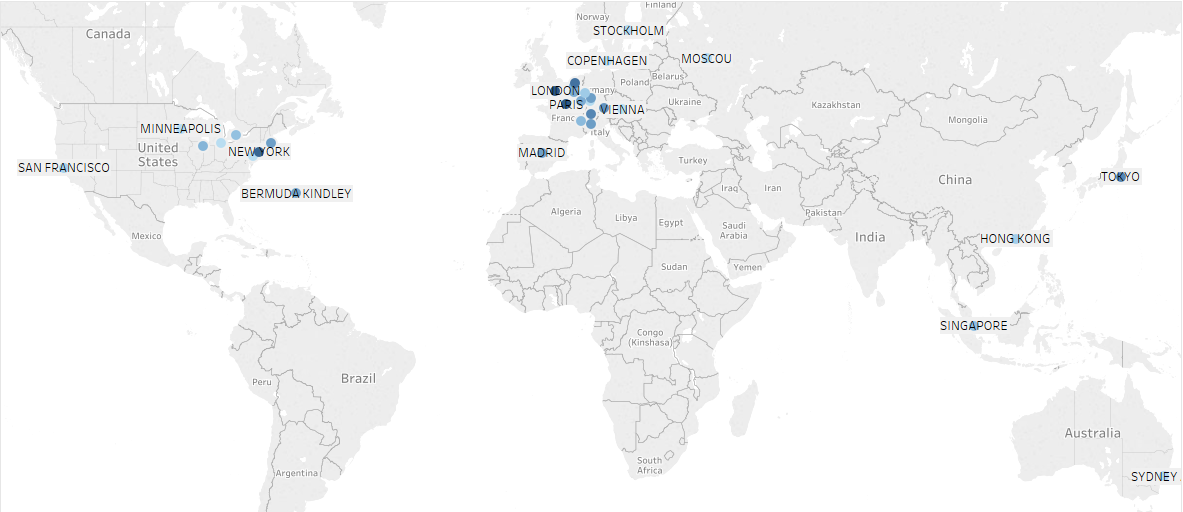
\includegraphics[width=1.0\linewidth]{city-networks-top-cumulative-map}
		\caption[Top economic cities on global map]{Top cities in the year 2010 and 2013 based on Cumulative Ranking.}
		\label{fig:city-networks-top-cumulative-map}
	\end{figure}
	
	\begin{figure}[ht]
		\centering
		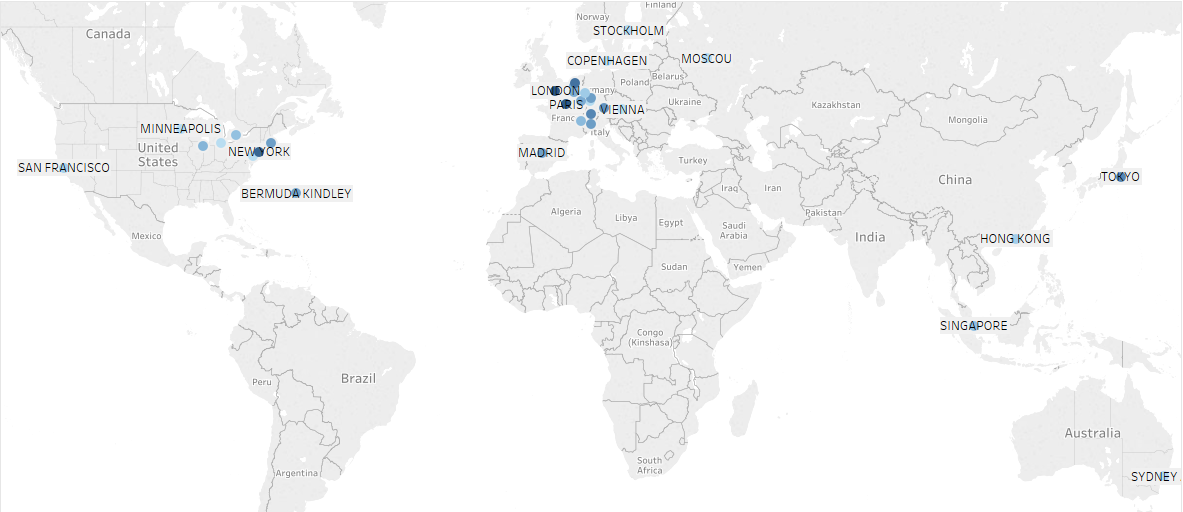
\includegraphics[width=1\linewidth]{city-networks-top-cumulative-map}
		\caption[Top economic cities with positive change on global map]{Top cities with positive change in cumulative rankings from 2010 to 2013.}
		\label{fig:city-networks-top-positive-cumulative-map}
	\end{figure}
	
	
	\begin{figure}[ht]
		\centering
		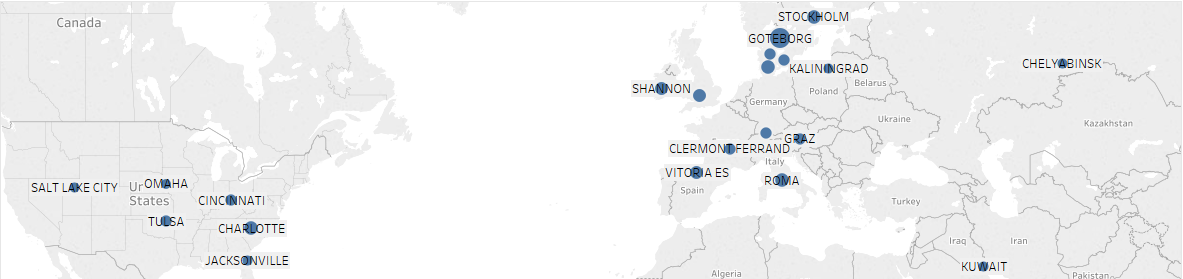
\includegraphics[width=1\linewidth]{city-networks-top-negative-cumulative-map}
		\caption[Top economic cities with negative change on global map]{Top cities with negative change in cumulative rankings from 2010 to 2013.}
		\label{fig:city-networks-top-negative-cumulative-map}
	\end{figure}

		\subsection{Supplementary comments}
		The cities with strongest development can be observed as spread out. In the Western Europe, we Mannheim and Haover from Germany, Jersey and Guernsey from the UK, Milan and Bologna from Italy, Antwerp from Belgium and Salzburg from Austria with positive growth. In the North American region, we see Kansas city, Tampa, Baltimore and Pheonix as good examples (in the US, these are not the top tier cities). On the East Asian front, we see that Beijing (China) is catching up with Hongkong, which outstripped Shanghai, the captal of China in economic and political movements. As for the Middle eastern Gulf region in Asia, Dubai and Abu Dhabi represent UAE and Cairo represents Egypt with all showing positive growth. There are some interesting observations as well, Akrotiri and Nicosia in Cyprus are outliers which might be developing due to Russian investments which transit into other European cities through these two. However, the intersting trend of developing nations showing strong growth continues as we see Rio De Jenario from Brazil, Istanbul from Turkey and Lagos fron Nigeria surfacing.
		
		In contrast, the declining cities which exhibit negative cumulative ranking appear mostly from USA, spread across East coast and central regions. Although most of these cities are not the strongest cities with respect to their presentation in multinational firms, we do see examples from Western Europe where traditionally strong economies lost their ranks. Friedrichshafen and Dortmund from Germany, Clermont-Ferrand and Annecy from France, Sonderborg and Copenhagen from Denmark, Goteborg and Stockholm from Sweden and Rome from Italy are such examples. Most interestingly, Kuwait City is an unexpected exception in this list.
		
		From these results, the most prominent findings we can draw are:
		
		\begin{enumerate}
			\item The cities which showed positive growth are spread across the world, contrary to common belief that the growth is concentrated only to some countries like China and Russia.
			
			\item The cities which were dominant in 2010 retaind their ranks in 2013 as well. The major change is mostly within the regions.
			
			\item Cities with highest decline in their ranks did not affect the globalization. They only lost their position within sub-regional system.
		\end{enumerate}
		
		The transformations we witness are within the regional sub-systems as highlighted by Rozenblat et. al. \cite{rozenblat2017}. Almost 3/4th of the ownerships of multinational links belong to North America, East Europe, Great Britain (alongside commonwealth countries), Japan, East Asia and India. The transformations do not change the regional dominance, but within the inner structure of regions. While we can clearly observe emergence of China and Middle East and declining trend in regions within US and Europe, some cities handled economic crisis comparatively better. This is also due to specialization functions of cities, some of which we enlist below:
		
		\begin{itemize}
			\item Swiss city Geneva is a highlight in finance domain with presence of most of the international banks and financial chains.
			
			\item Baltimore in USA, which has the highest positive change is a headquarter of high-tech industry.
			
			\item The island of Jersey, which is considered as a leading offshore financial city, is continually growing due to economic activity in financial sector.
			
			\item German city Mannheim, which showed positive growth is a well-known hub of medical technology innovations. The headquarters of several giants in medical tech, such as Siemens Healthcare and Roche Diagnostics are hosted in Mannheim. Another strong driving force causing the growth of Mannheim and some other German cities is the transport sector (Volkswagan).
			
			\item In Italy, Bolonga gains a spike due to boost in car manufacturing business. Ferrari, Ducati and Lamborghini to name a few manufacturers.
			
			\item Dubai, Abu Dhabi from UAE have diversified their economy in air transport, finance and technology. This diversification made them resilient to economic cisis and emerge as growing cities.
			
			\item Cairo (Egypt) and Lagos (Nigeria) are rising stars of Africa due to their integration with other global regions. Egpyt enjoys bounties from Suez canal and works as a bridge between Middle East and Africa.
			
		\end{itemize}
		
		The rise of Beijing and Shanghai, and the consecutive fall of Hongkong is no surprise. These reside in the same region and as foreseen, the disbalance occurs within the region more than external to it.
		
		The cities which declined steeply were due to some out of norm cause.For example, Swedish city Goteborg was hit by high unemployment due to its worst economic crisis in 2009; Ericsson and Volvo, the primary employers were the ones that faced the crisis the most. It only started recovering slowly from 2014, and is gaining its position back. Stockholm, the Swedish capital is another example which faced a drop during 2010 and 2013 after steady growth from 2008 to 2010. But from 2014 and onwards, we see Sweden's GDP to reflect a higher growth than most of regions in UK and Europe. Stockholm’s success stems from five major sectors, Trade in high-tech industries (refined petroleum products, electronics, chemicals, and transportation equipment), Innovation with a high number of patents with commercial and university-industry partnerships, Talent with highly educated work-force, Infrastructure (top quality freight, aviation, and broadband systems) and Governance which ensures that the policies support business success. Another examples comes from Denish city Sodenborg, which is a key player in heating and cooling products; this city is facing decline mainly due to overall decrease in GDP, as the growth in 2016 is reported to be 1.1\% only. In this case, the country's economy contributed to decline of city's economy.
	

	\section{The Influence Mining Framework}
	\label{sec:appendix-C-inf-framework}
	
	\begin{figure}[H]
		\begin{multicols}{2}
			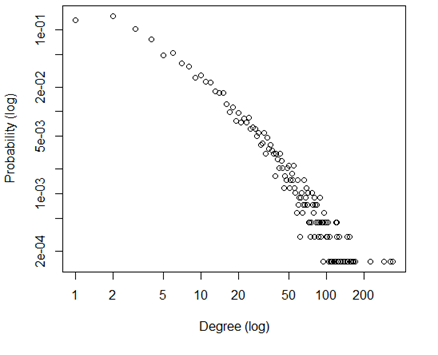
\includegraphics[width=\linewidth]{degree-distribution-arxiv}\par 
			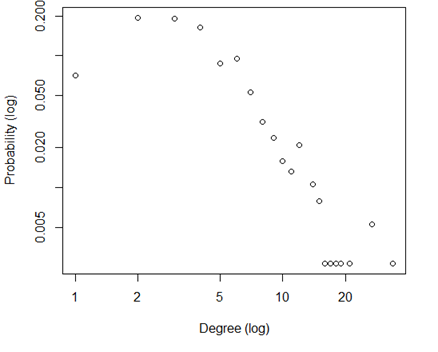
\includegraphics[width=\linewidth]{degree-distribution-author}\par 
		\end{multicols}
		\begin{multicols}{2}
			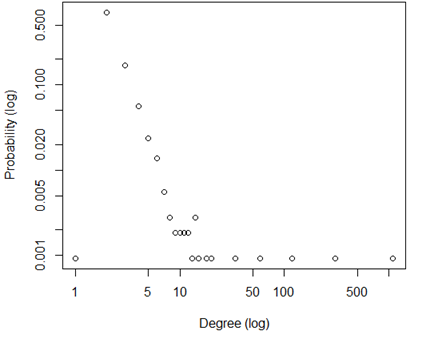
\includegraphics[width=\linewidth]{degree-distribution-automata}\par 
			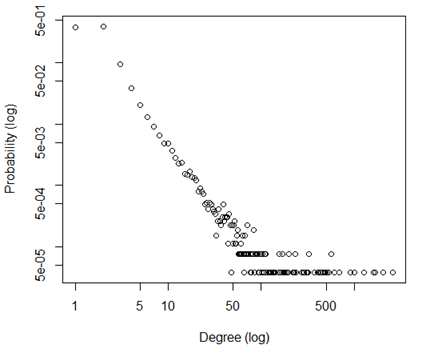
\includegraphics[width=\linewidth]{degree-distribution-caida}\par 
		\end{multicols}
		\begin{multicols}{2}
			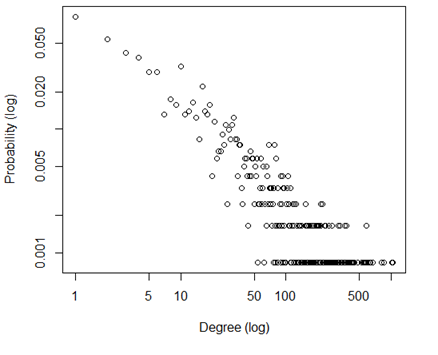
\includegraphics[width=\linewidth]{degree-distribution-city2010}\par 
			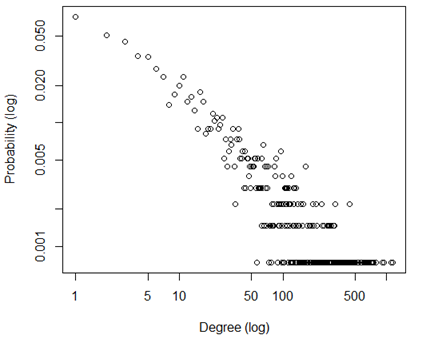
\includegraphics[width=\linewidth]{degree-distribution-city2013}\par 
		\end{multicols}
		\caption[Degree distribution log-log plots (1)]{Degree distribution log-log plots. ArXiv collaboration (arxiv) on Top-Left; Author NetScience (author) on Top-Right; Automata GraphDraw (automata) on Center-Left; AS-Caida (caida) on Center-Right; City Economic Networks (city2010) on Bottom-Left; City Economic Networks (city2013) on Bottom-Right}
		\label{fig:inf-framework-networks1}
	\end{figure}
	
	\begin{figure}[H]
		\begin{multicols}{2}
			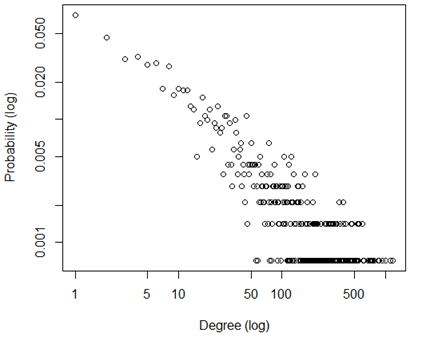
\includegraphics[width=\linewidth]{degree-distribution-city2016}\par 
			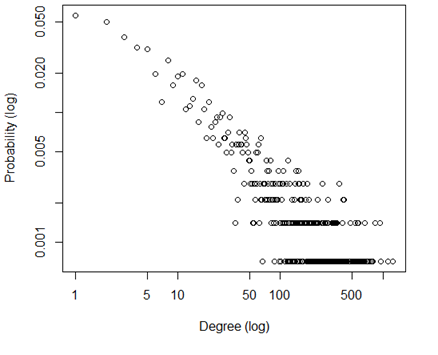
\includegraphics[width=\linewidth]{degree-distribution-city2019}\par 
		\end{multicols}
		\begin{multicols}{2}
			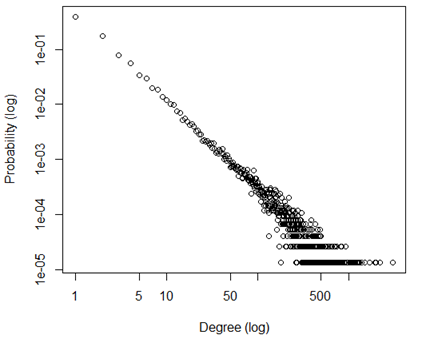
\includegraphics[width=\linewidth]{degree-distribution-epinions}\par 
			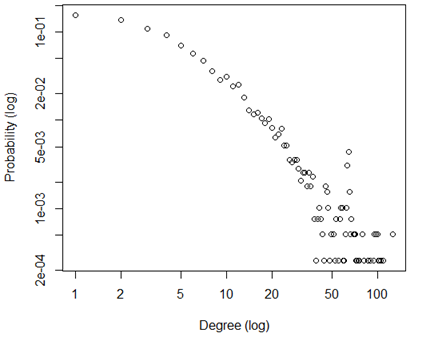
\includegraphics[width=\linewidth]{degree-distribution-fb_tvshows}\par 
		\end{multicols}
		\begin{multicols}{2}
			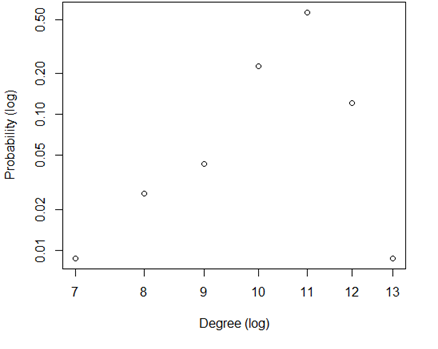
\includegraphics[width=\linewidth]{degree-distribution-football}\par 
			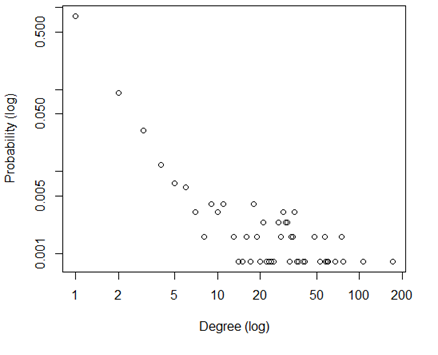
\includegraphics[width=\linewidth]{degree-distribution-influence_citation}\par 
		\end{multicols}
		\caption[Degree distribution log-log plots (2)]{City Economic Networks (city2016) on Top-Left; City Economic Networks (city2019) on Top-Right; Epinions.com (epinions) on Center-Left; Facebook TV shows (fb\_tvshows) on Center-Right; Football games (football) on Bottom-Left; Influence citations (influence\_citation) on Bottom-Right}
		\label{fig:inf-framework-networks2}
	\end{figure}
	
	\begin{figure}[H]
		\begin{multicols}{2}
			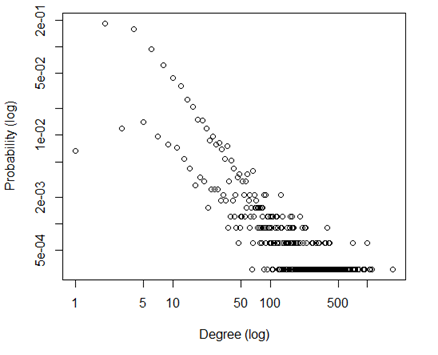
\includegraphics[width=\linewidth]{degree-distribution-ita2000}\par 
			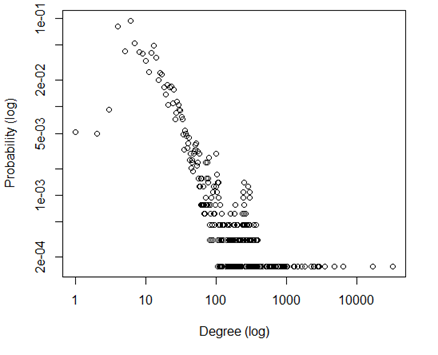
\includegraphics[width=\linewidth]{degree-distribution-jdk6}\par 
		\end{multicols}
		\begin{multicols}{2}
			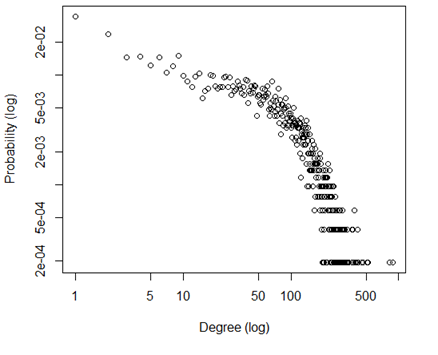
\includegraphics[width=\linewidth]{degree-distribution-johnshopkins}\par 
			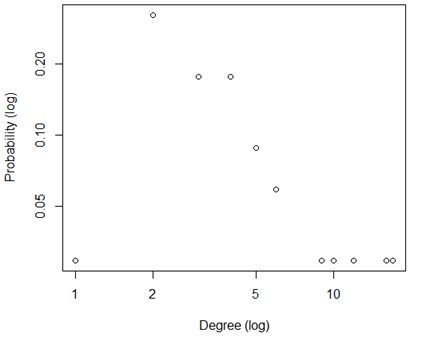
\includegraphics[width=\linewidth]{degree-distribution-karate}\par 
		\end{multicols}
		\begin{multicols}{2}
			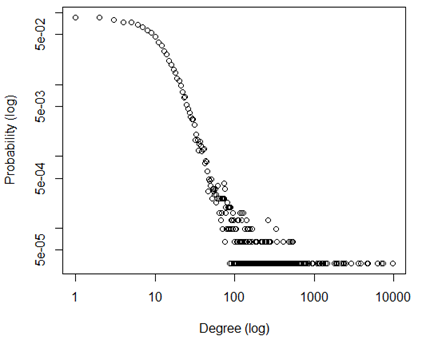
\includegraphics[width=\linewidth]{degree-distribution-linux}\par 
			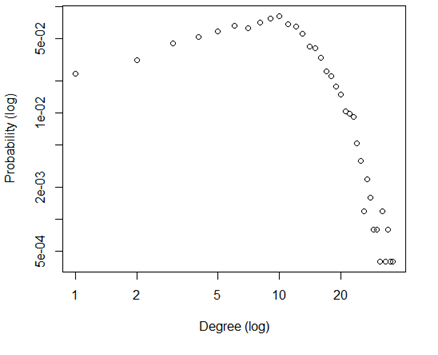
\includegraphics[width=\linewidth]{degree-distribution-moreno}\par 
		\end{multicols}
		\caption[Degree distribution log-log plots (3)]{ITA-2000 (ita2000) on Top-Left; Java Development Kit 6 Classes(jdk6) on Top-Right; Johns Hopkins University Facbook Network (johnshopkins) on Center-Left; Karate club (karate) on Center-Right; Linux source code (linux) on Bottom-Left; Moreno Student–student friendships (moreno) on Bottom-Right}
		\label{fig:inf-framework-networks3}
	\end{figure}
	
	\begin{figure}[H]
		\begin{multicols}{2}
			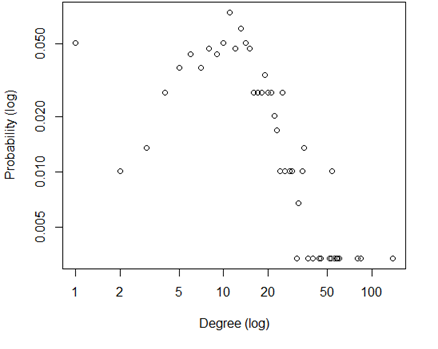
\includegraphics[width=\linewidth]{degree-distribution-nematode}\par 
			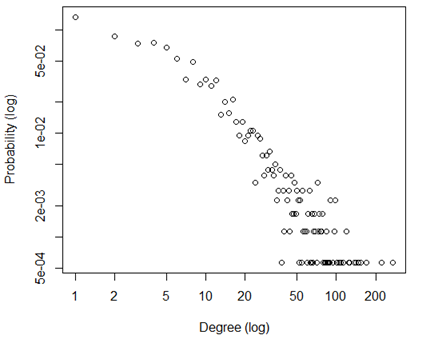
\includegraphics[width=\linewidth]{degree-distribution-hamster}\par 
		\end{multicols}
		\begin{multicols}{2}
			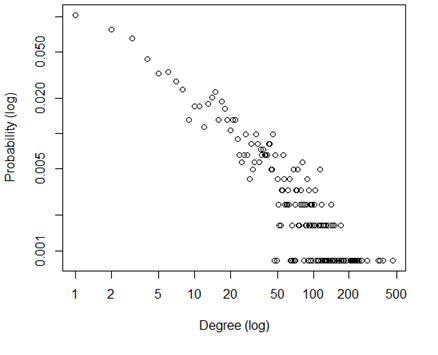
\includegraphics[width=\linewidth]{degree-distribution-political}\par 
			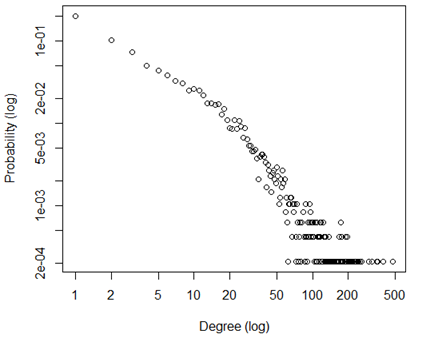
\includegraphics[width=\linewidth]{degree-distribution-spam}\par 
		\end{multicols}
		\begin{multicols}{2}
			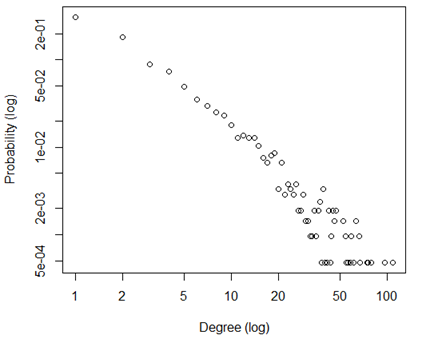
\includegraphics[width=\linewidth]{degree-distribution-routers}\par 
			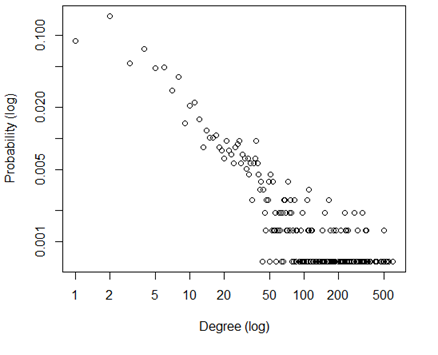
\includegraphics[width=\linewidth]{degree-distribution-usairport}\par 
		\end{multicols}
		\caption[Degree distribution log-log plots (4)]{Neural Network of Nematode (nematode) on Top-Left; Petster-hamster (hamster) on Top-Right; Political Blogs (political) on Center-Left; Spam on Web Challenge (spam) on Center-Right; Tech Routers(routers) on Bottom-Left; US Airport (usairport) on Bottom-Right}
		\label{fig:inf-framework-networks4}
	\end{figure}
	
	\begin{figure}[H]
		\begin{multicols}{2}
			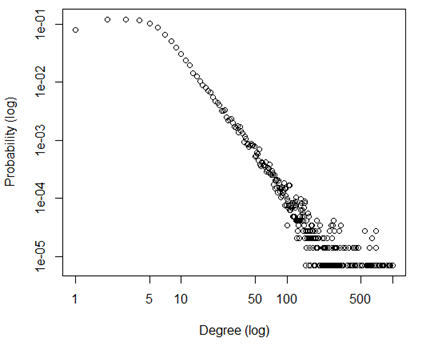
\includegraphics[width=\linewidth]{degree-distribution-wordnet}\par 
			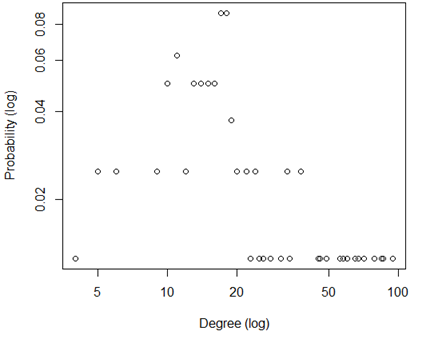
\includegraphics[width=\linewidth]{degree-distribution-world_trade}\par 
		\end{multicols}
		\begin{multicols}{1}
			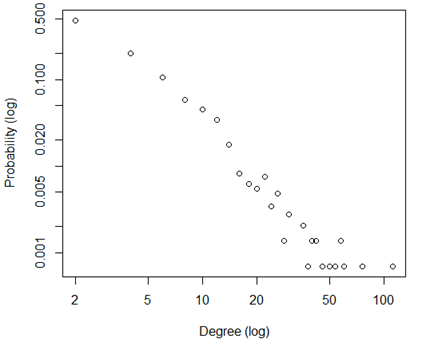
\includegraphics[width=\linewidth]{degree-distribution-protein}\par 
		\end{multicols}
		\caption[Degree distribution log-log plots (5)]{Word Net (wordnet) on Top-Left; World Trade (world\_trade) on Top-Right; Yeast Protein (protein) on Bottom-Left.}
		\label{fig:inf-framework-networks5}
	\end{figure}

		\subsection{Analysis of Dataset}
		\label{subsec:appendix-dataset-analysis}
		
		\begin{figure}[H]
			\centering
			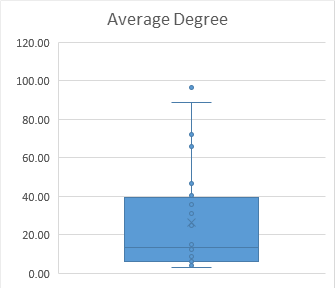
\includegraphics[width=0.7\textwidth]{inf-framework-networks-avg-degree}
			\caption{Boxplot of average degrees of the networks.}
			\label{fig:inf-framework-networks-avg-degree}
		\end{figure}
		
		\begin{figure}[H]
			\centering
			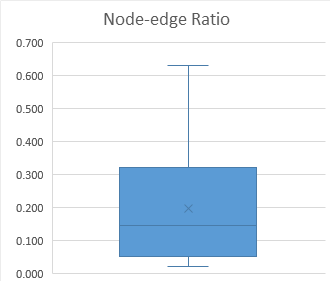
\includegraphics[width=0.7\textwidth]{inf-framework-networks-ratio}
			\caption{Boxplot of Node-edge ratios of the networks.}
			\label{fig:inf-framework-networks-ratio}
		\end{figure}
		
		\begin{figure}[H]
			\centering
			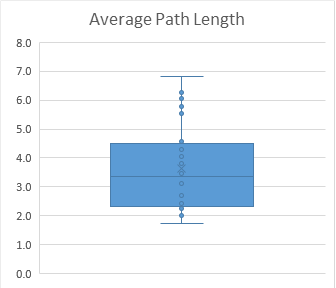
\includegraphics[width=0.7\textwidth]{inf-framework-networks-apl}
			\caption{Boxplot of Average Path Lengths of the networks.}
			\label{fig:inf-framework-networks-apl}
		\end{figure}
		
		\begin{figure}[H]
			\centering
			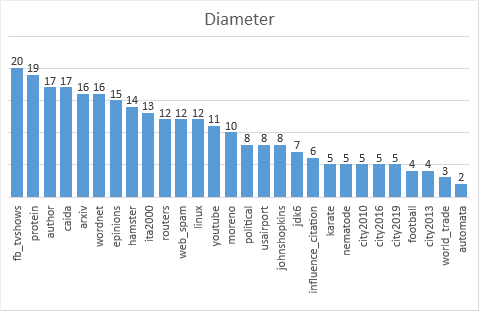
\includegraphics[width=0.7\textwidth]{inf-framework-networks-diameter}
			\caption{Diameters of the networks in descending order.}
			\label{fig:inf-framework-networks-diameter}
		\end{figure}
		
		On transitivity, only fb\_tvshows has an unusually high value of transitivity (0.59), the networks are majorly ranging between 0.15 and 0.35 (see Figure \ref{fig:inf-framework-networks-transitivity}). The higher value means tighter clique-like structure.
		
		\begin{figure}[H]
			\centering
			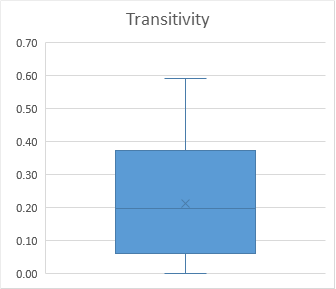
\includegraphics[width=0.7\textwidth]{inf-framework-networks-transitivity}
			\caption{Boxplot of Transitivity of the networks.}
			\label{fig:inf-framework-networks-transitivity}
		\end{figure}
		
		Assortativity is a unique metric which is used to understand dynamic properties of a graph, for example against a targeted attack a highly assortative network will be infected completely differently than a low assortative network. We note that the data set covers a wide spectrum of networks with a few highly assortative, few highly disassortative, and several low assortative/disassortative networks; this is shown in histogram \ref{fig:inf-framework-networks-assortativity}.
		
		\begin{figure}[H]
			\centering
			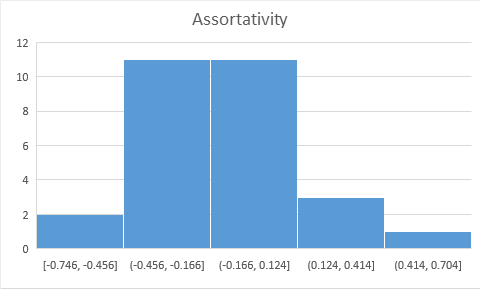
\includegraphics[width=0.7\textwidth]{inf-framework-networks-assortativity}
			\caption{Histogram of Assortativity of the networks.}
			\label{fig:inf-framework-networks-assortativity}
		\end{figure}
		
		Looking at the power-law, the minimum, mean, maximum and outlier values are 1.69, 3.23, 8.42, 21.19 respectively. Thus indicating that most of the networks follow power-law distribution. All the distribution plots %todo distribution plots of what? degree? 
		can be found in Appendix \ref{sec:appendix-C-inf-framework}.
		
		In a nutshell, the selection of networks ensures that the results will not be biased by networks with any specific structure. %and focus on only one or two types of complex networks.

		\subsection{Evaluation results of IMine framework}
		\label{subsec:appendix-imine-evaluation}
		
		\begin{figure}[H]
			\centering
			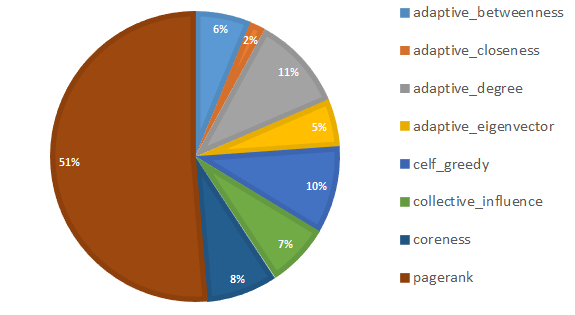
\includegraphics[width=0.75\textwidth]{inf-summary-budget-influence-ic}
			\caption[IMine performance on budget criteria for Influence\_IC test]{Percentage of number of instances each method outperformed the other methods for INFLUENCE\_IC test in budget criteria. The method with highest influence was selected as the best method. Pagerank ranked top (51\%), followed by CELF-greedy (10\%), while Adaptive Closeness performed worst (2\%).}
			\label{fig:inf-summary-budget-influence-ic}
		\end{figure}
		
		\begin{figure}[H]
			\centering
			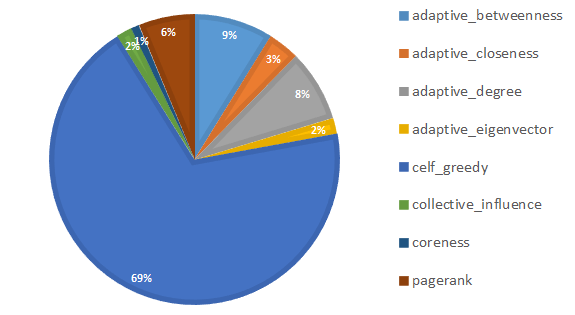
\includegraphics[width=0.75\textwidth]{inf-summary-budget-influence-lt}
			\caption[IMine performance on budget criteria for Influence\_LT test]{Percentage of number of instances each method outperformed the other methods for INFLUENCE\_LT test in budget criteria. The method with most highest was selected as the best method. As clearly shown, CELF-greedy outperformed all other methods by a wide margin (69\%), where Coreness performed poorer than all (1\%).}
			\label{fig:inf-summary-budget-influence-lt}
		\end{figure}
		
		\begin{figure}[H]
			\centering
			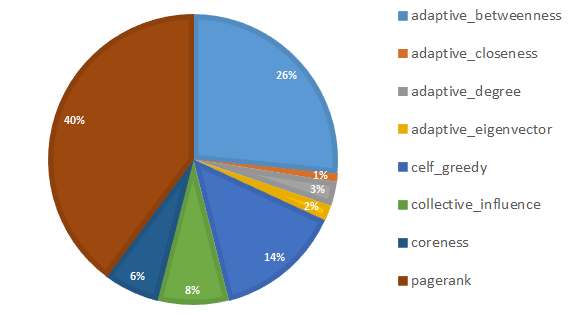
\includegraphics[width=1\textwidth]{inf-summary-budget-resilience}
			\caption[IMine performance on budget criteria for Resilience test]{Percentage of number of instances each method outperformed the other methods for RESILIENCE test in budget criteria. The method with most highest was selected as the best method. Pagerank turned out to be top performer in the trails (40\%), followed by Adaptive Betweenness (26\%), where Adaptive Closeness ranked last (1\%).}
			\label{fig:inf-summary-budget-resilience}
		\end{figure}
		
		\begin{figure}[H]
			\centering
			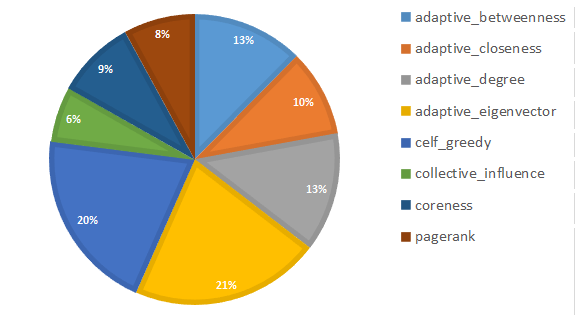
\includegraphics[width=1\textwidth]{inf-summary-influence-influence-ic}
			\caption[IMine performance on influence criteria for Influence\_IC test]{Percentage of number of instances each method outperformed the other methods for INFLUENCE\_IC test in influence criteria. The method with most highest was selected as the best method. }
			\label{fig:inf-summary-influence-influence-ic}
		\end{figure}
		
		\begin{figure}[H]
			\centering
			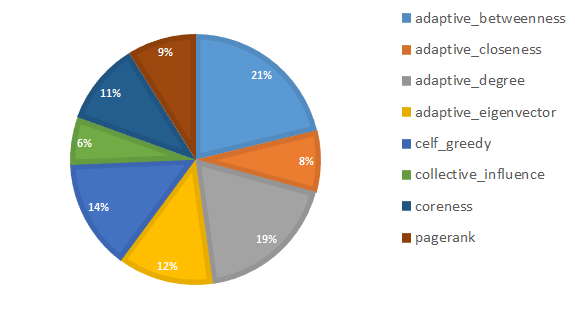
\includegraphics[width=1\textwidth]{inf-summary-influence-influence-lt}
			\caption[IMine performance on influence criteria for Influence\_LT test]{Percentage of number of instances each method outperformed the other methods for INFLUENCE\_LT test in influence criteria. The method with most highest was selected as the best method.}
			\label{fig:inf-summary-influence-influence-lt}
		\end{figure}
		
		\begin{figure}[H]
			\centering
			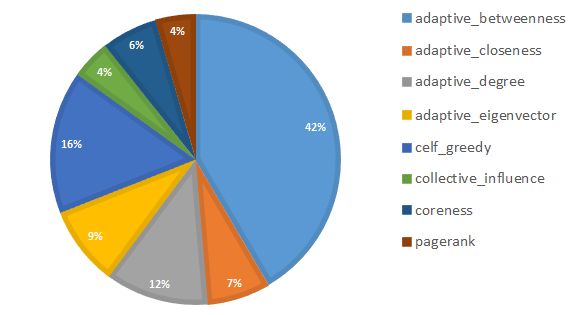
\includegraphics[width=1\textwidth]{inf-summary-influence-resilience}
			\caption[IMine performance on budget criteria for Resilience test]{Percentage of number of instances each method outperformed the other methods for RESILIENCE test in influence criteria. The method with most highest was selected as the best method.}
			\label{fig:inf-summary-influence-resilience}
		\end{figure}
		
		
		% *** arxiv ***
		\begin{figure*}[ht]
			\begin{multicols}{2}
				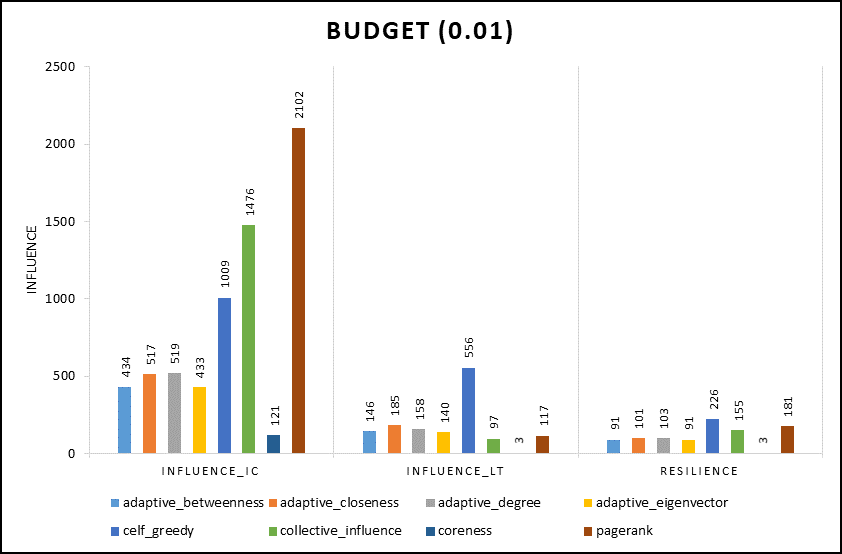
\includegraphics[angle=90, scale=0.65]{arxiv-budget-1}\par 
				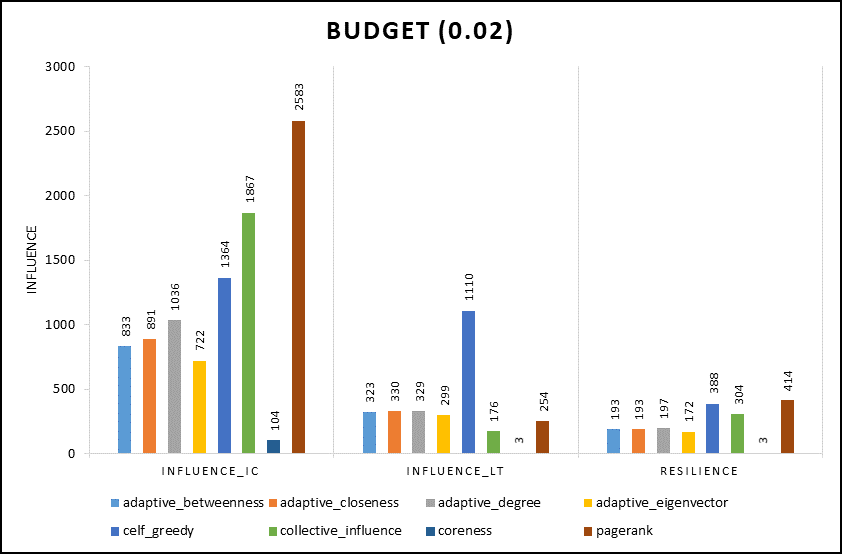
\includegraphics[angle=90, scale=0.65]{arxiv-budget-2}\par 
			\end{multicols}
			\begin{multicols}{2}
				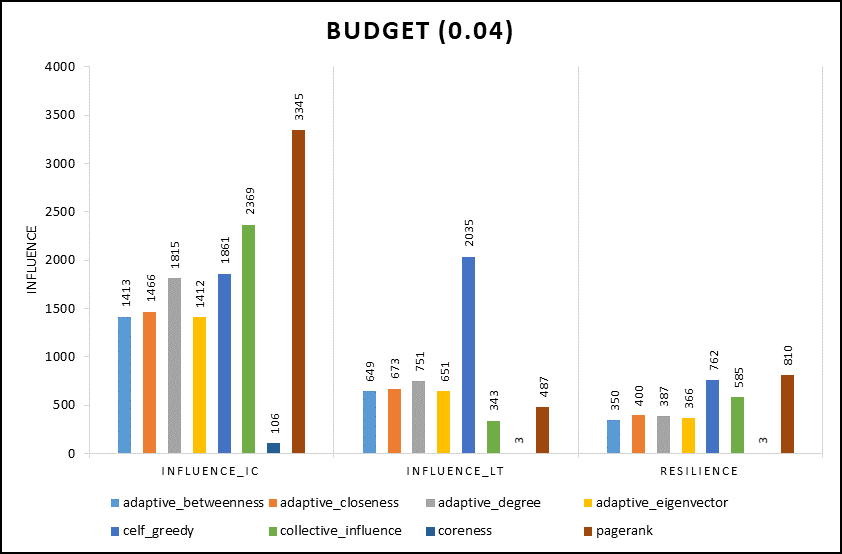
\includegraphics[angle=90, scale=0.65]{arxiv-budget-4}\par 
				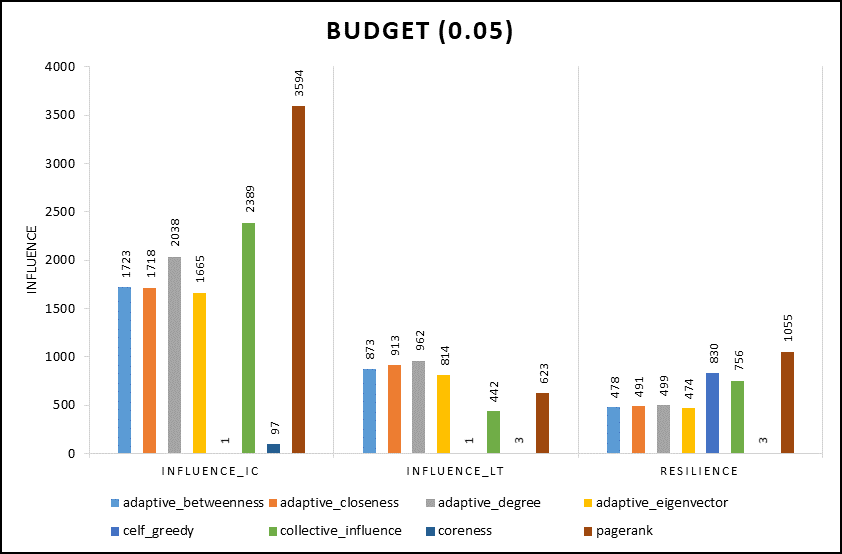
\includegraphics[angle=90, scale=0.65]{arxiv-budget-5}\par 
			\end{multicols}
			
			\caption{Influence measure of Arxiv network on range on all budgets evaluated for all three tests.}
			\label{fig:inf-framework-arxiv}
		\end{figure*}
		
		\begin{figure*}[ht]
			\begin{multicols}{2}
				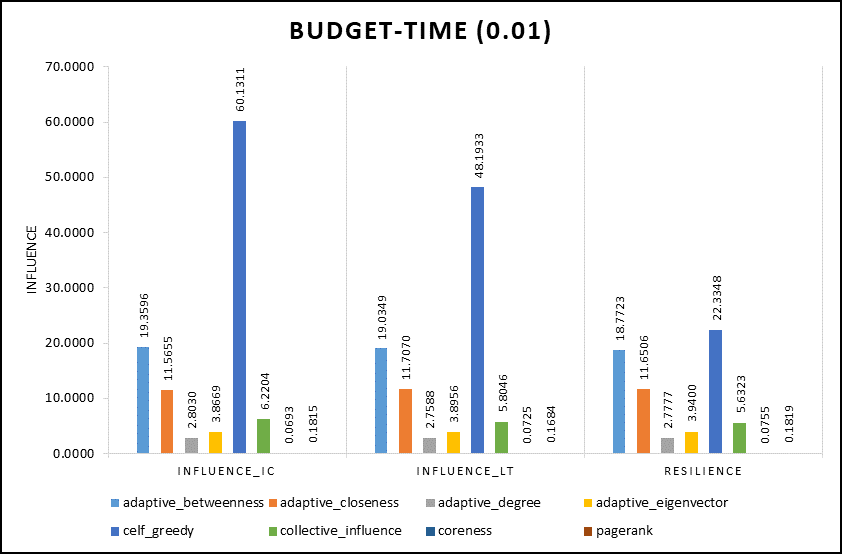
\includegraphics[angle=90, scale=0.65]{arxiv-budget-time-1}\par 
				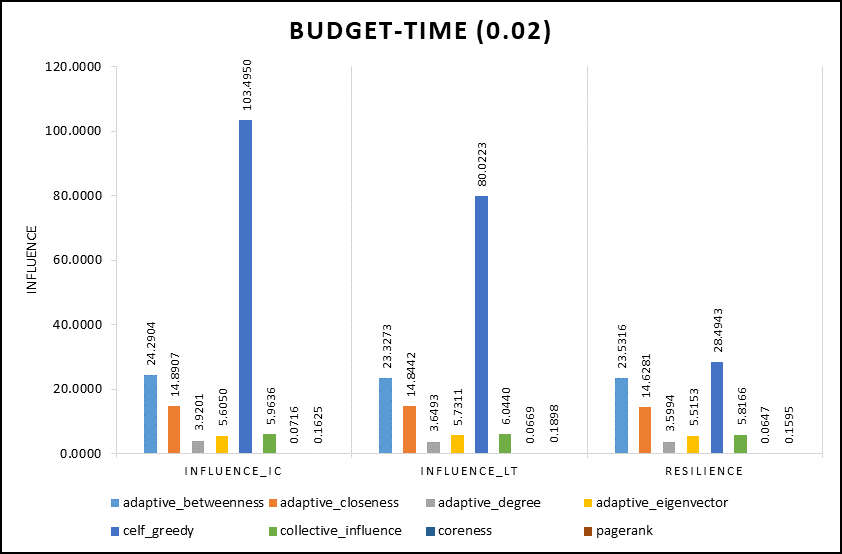
\includegraphics[angle=90, scale=0.65]{arxiv-budget-time-2}\par 
			\end{multicols}
			\begin{multicols}{2}
				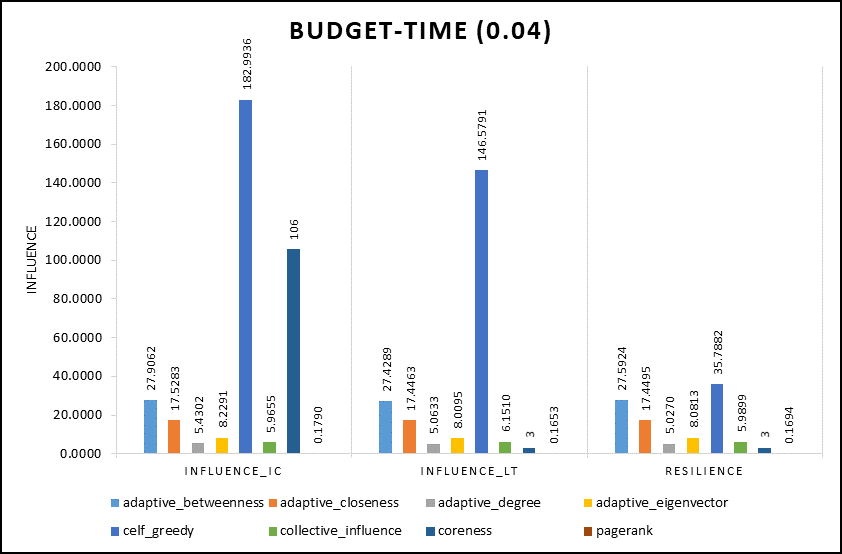
\includegraphics[angle=90, scale=0.65]{arxiv-budget-time-4}\par 
				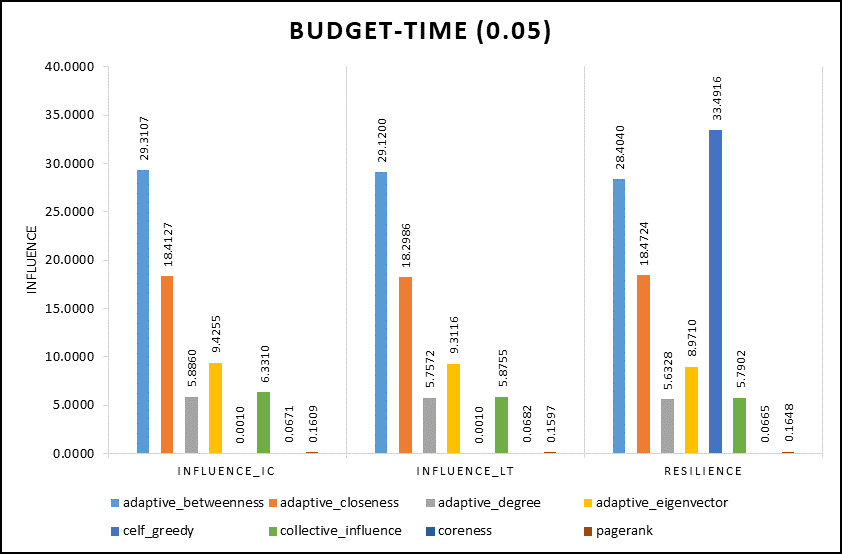
\includegraphics[angle=90, scale=0.65]{arxiv-budget-time-5}\par 
			\end{multicols}
			
			\caption{Normalized elapsed time for budget criteria on Arxiv network.}
			\label{fig:inf-framework-arxiv2}
		\end{figure*}
		
		\begin{figure*}[h]
			\begin{multicols}{2}
				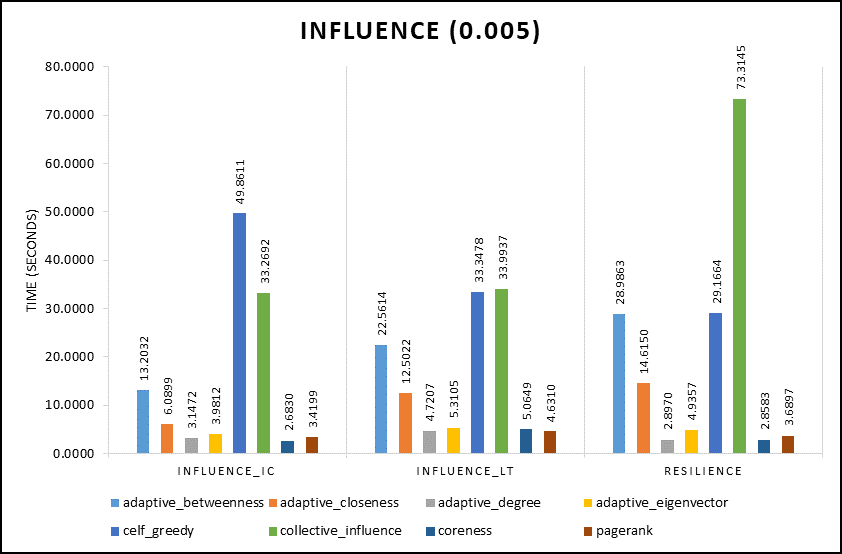
\includegraphics[angle=90, scale=0.65]{arxiv-influence-1}\par 
				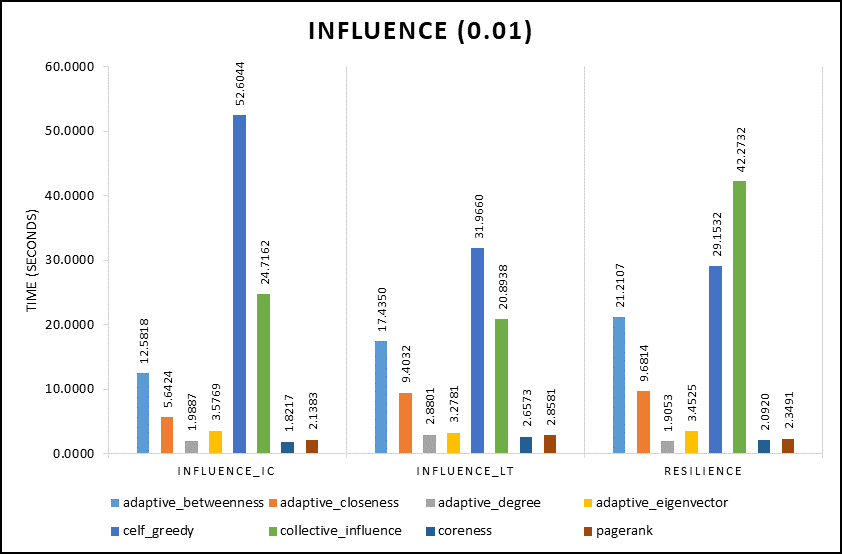
\includegraphics[angle=90, scale=0.65]{arxiv-influence-2}\par 
			\end{multicols}
			\begin{multicols}{2}
				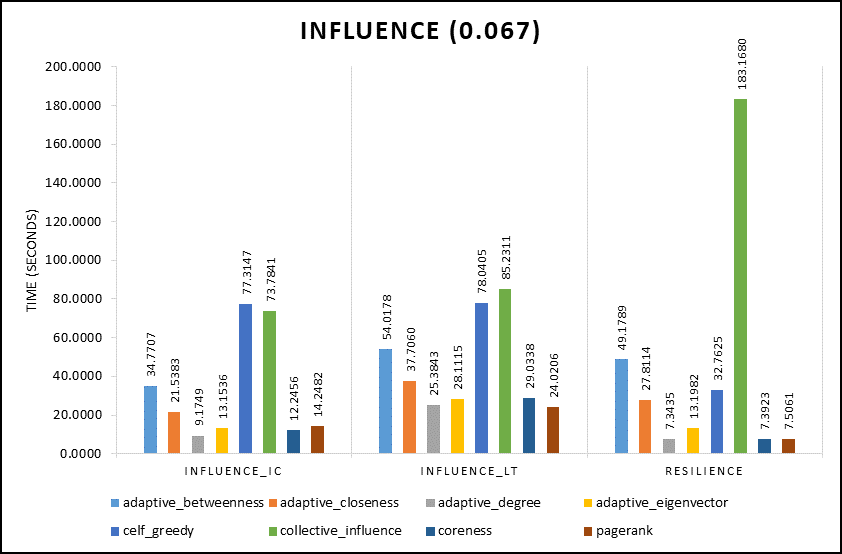
\includegraphics[angle=90, scale=0.65]{arxiv-influence-4}\par 
				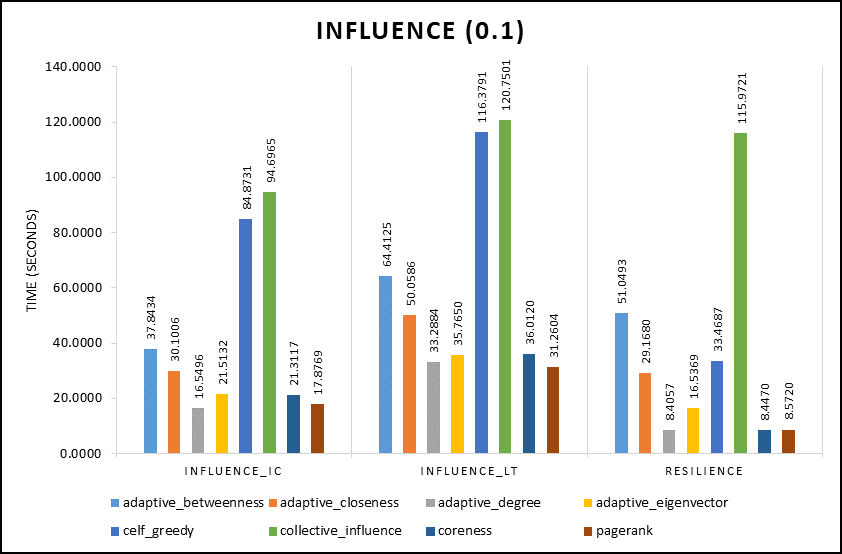
\includegraphics[angle=90, scale=0.65]{arxiv-influence-5}\par 
			\end{multicols}
			
			\caption{Normalized elapsed time for influence criteria on Arxiv network.}
			\label{fig:inf-framework-arxiv3}
		\end{figure*}
		
		
		% *** author ***
		\begin{figure*}[ht]
			\begin{multicols}{2}
				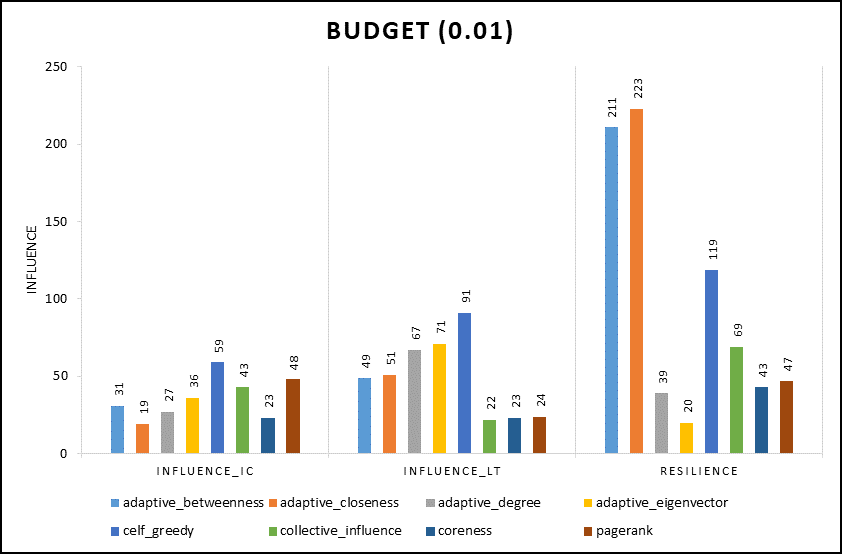
\includegraphics[angle=90, scale=0.65]{author-budget-1}\par 
				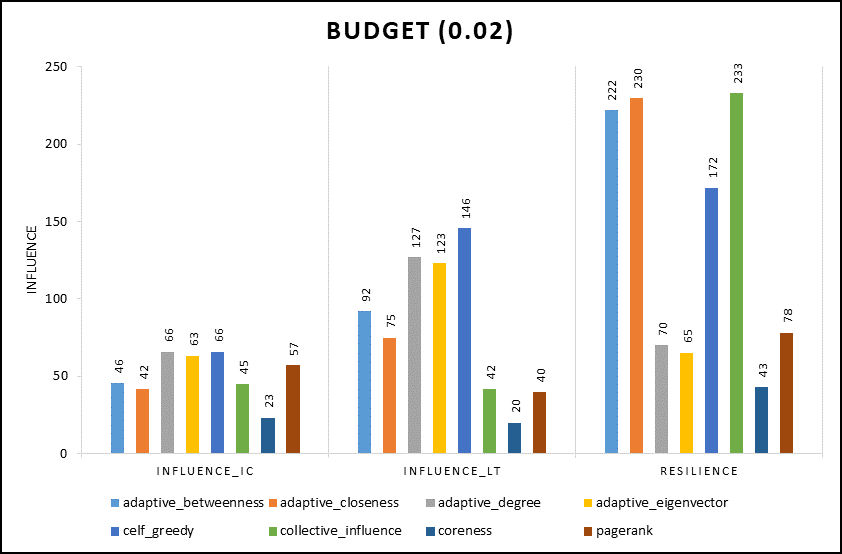
\includegraphics[angle=90, scale=0.65]{author-budget-2}\par 
			\end{multicols}
			\begin{multicols}{2}
				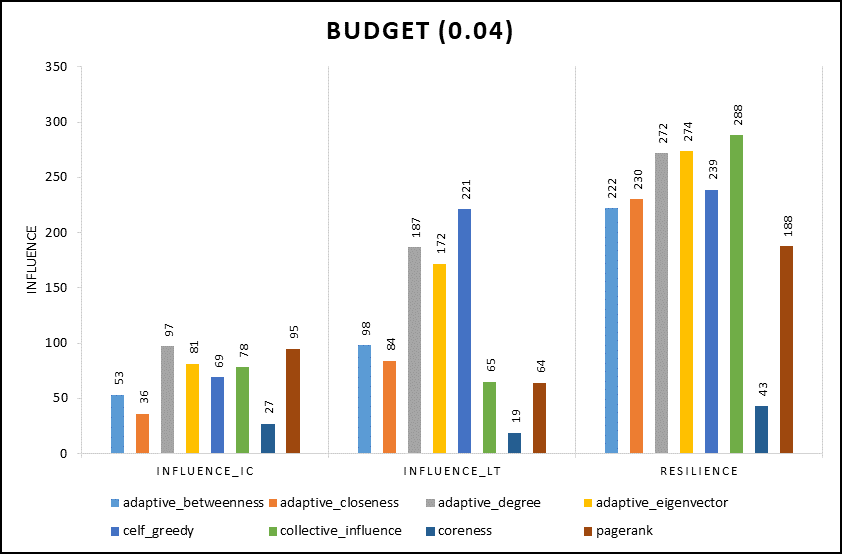
\includegraphics[angle=90, scale=0.65]{author-budget-4}\par 
				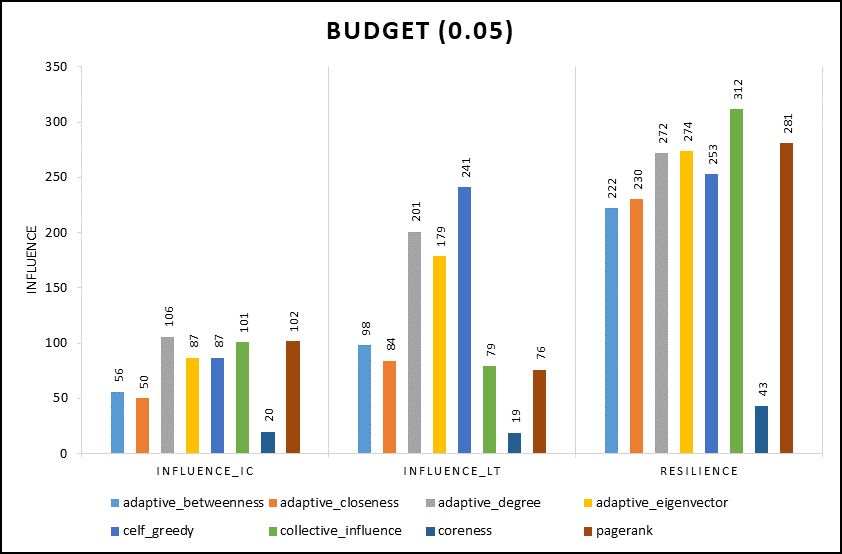
\includegraphics[angle=90, scale=0.65]{author-budget-5}\par 
			\end{multicols}
			
			\caption{Influence measure of Co-authorship network on range on all budgets evaluated for all three tests.}
			\label{fig:inf-framework-author}
		\end{figure*}
		
		\begin{figure*}[ht]
			\begin{multicols}{2}
				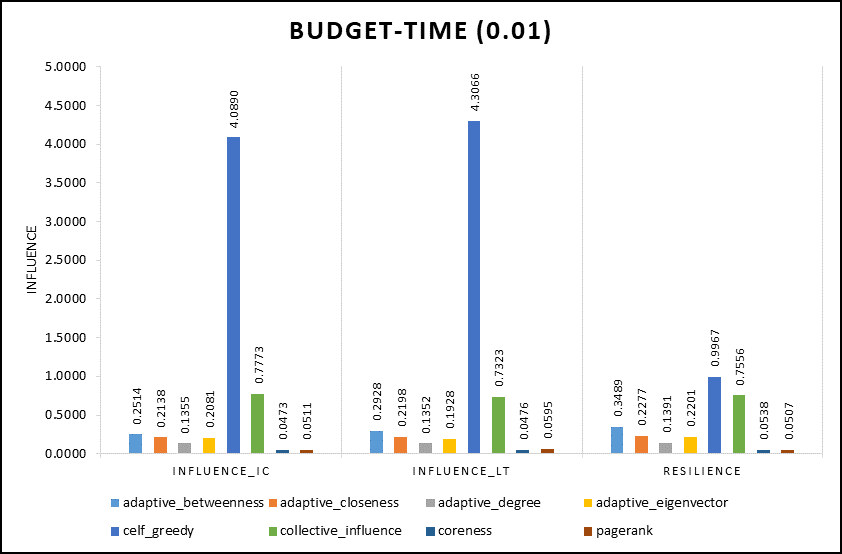
\includegraphics[angle=90, scale=0.65]{author-budget-time-1}\par 
				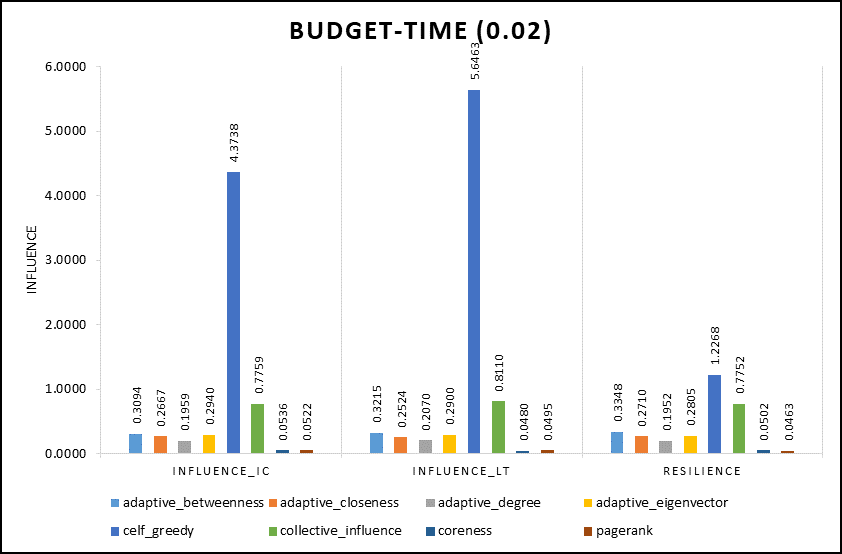
\includegraphics[angle=90, scale=0.65]{author-budget-time-2}\par 
			\end{multicols}
			\begin{multicols}{2}
				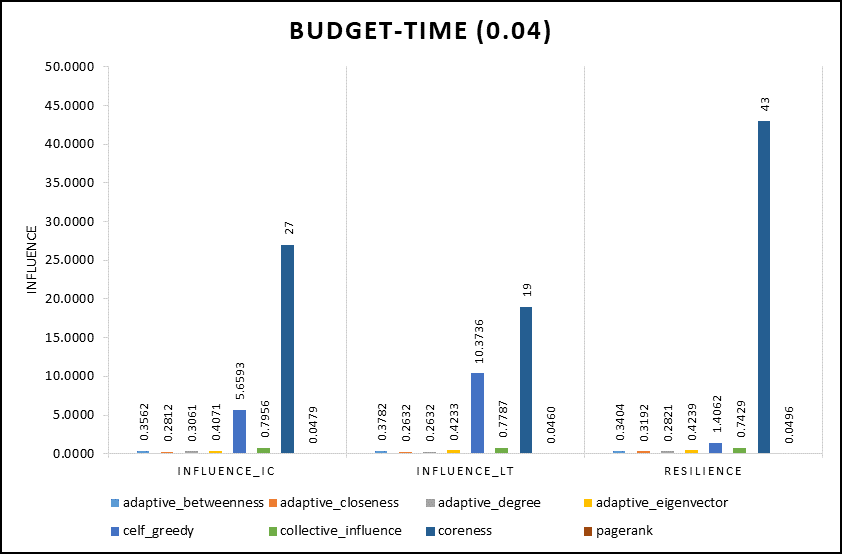
\includegraphics[angle=90, scale=0.65]{author-budget-time-4}\par 
				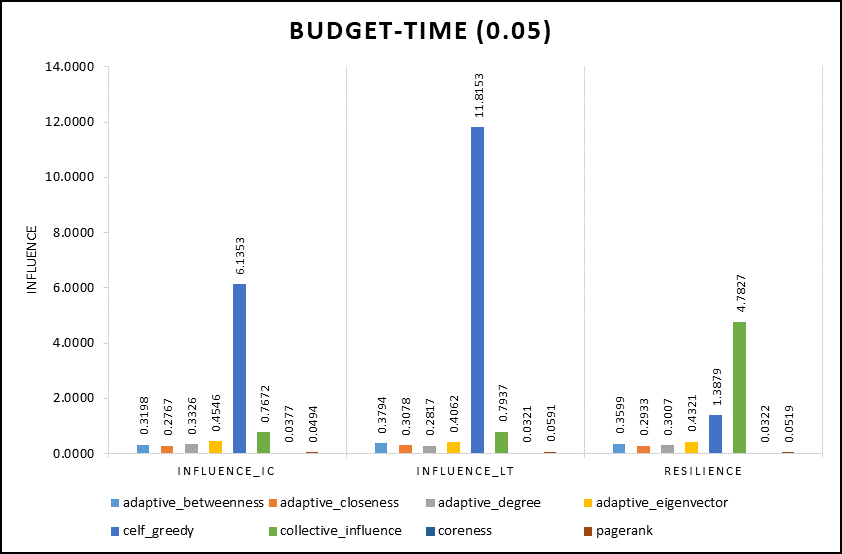
\includegraphics[angle=90, scale=0.65]{author-budget-time-5}\par 
			\end{multicols}
			
			\caption{Normalized elapsed time for budget criteria on Co-authorship network.}
			\label{fig:inf-framework-author2}
		\end{figure*}
		
		\begin{figure*}[h]
			\begin{multicols}{2}
				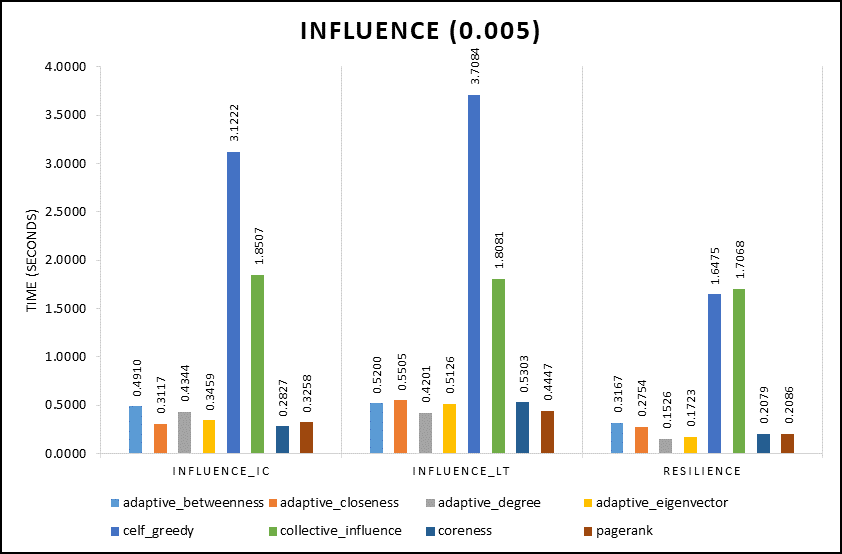
\includegraphics[angle=90, scale=0.65]{author-influence-1}\par 
				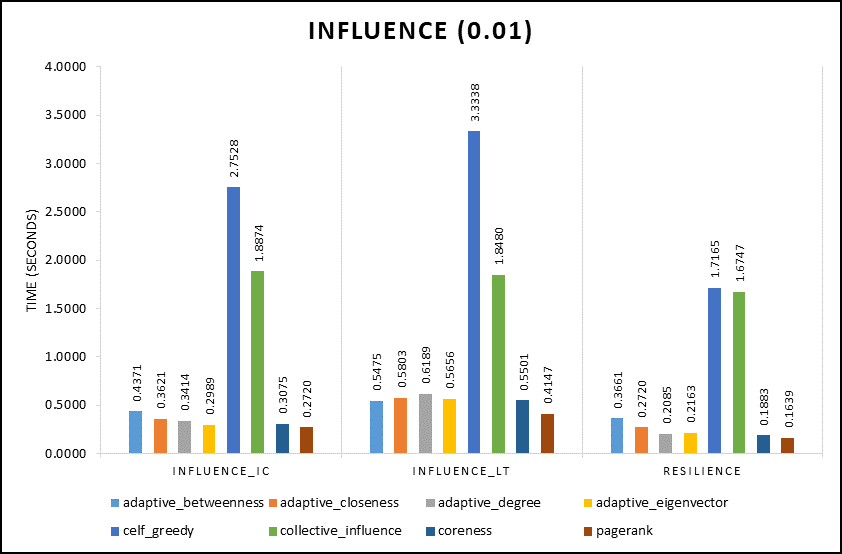
\includegraphics[angle=90, scale=0.65]{author-influence-2}\par 
			\end{multicols}
			\begin{multicols}{2}
				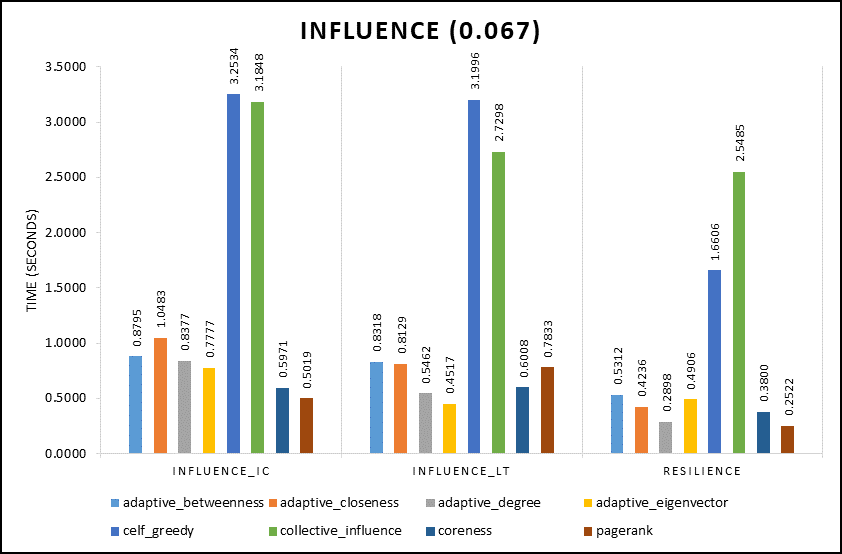
\includegraphics[angle=90, scale=0.65]{author-influence-4}\par 
				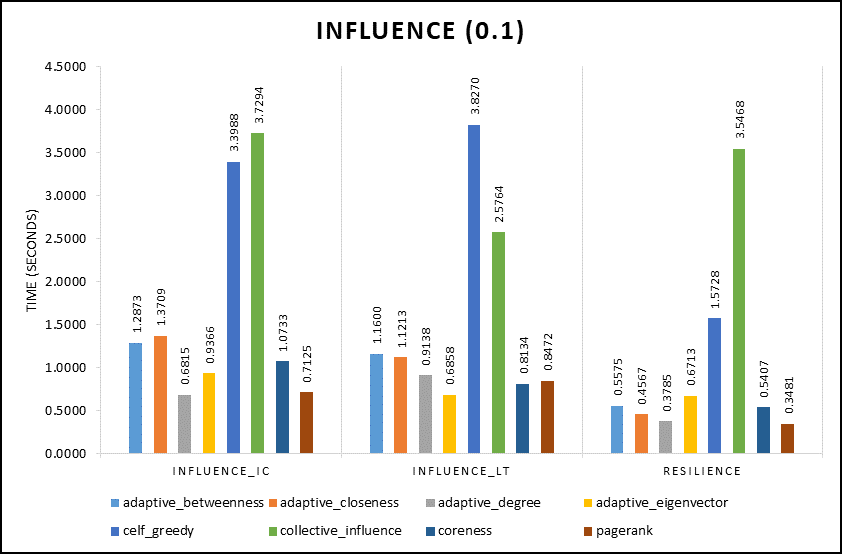
\includegraphics[angle=90, scale=0.65]{author-influence-5}\par 
			\end{multicols}
			
			\caption{Normalized elapsed time for influence criteria on Co-authorship network.}
			\label{fig:inf-framework-author3}
		\end{figure*}
		
		
		% *** automata ***
		\begin{figure*}[ht]
			\begin{multicols}{2}
				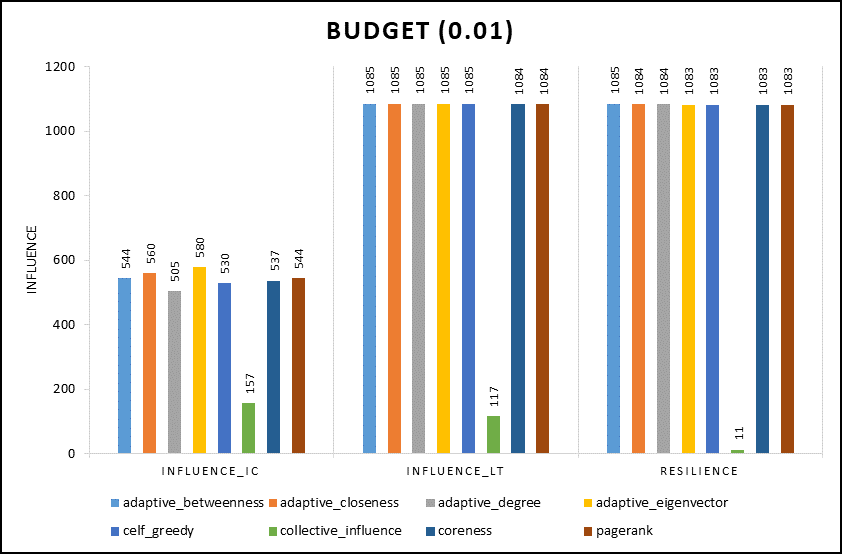
\includegraphics[angle=90, scale=0.65]{automata-budget-1}\par 
				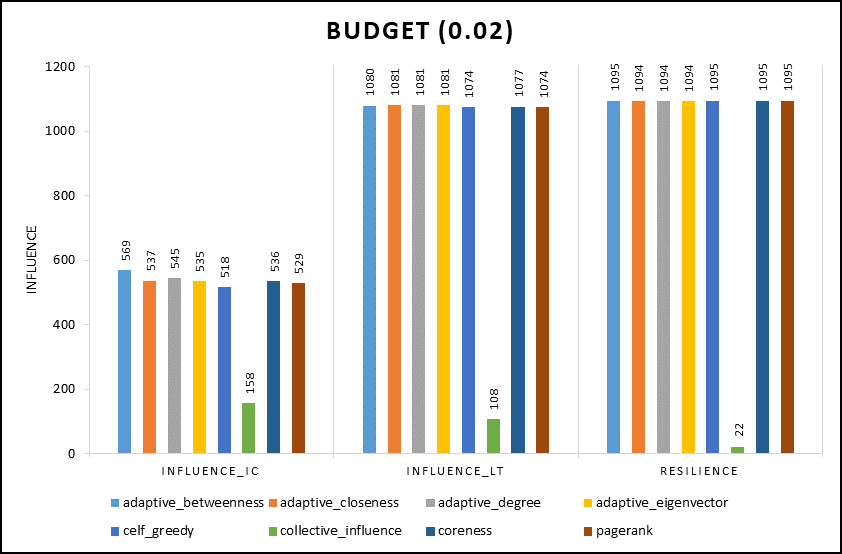
\includegraphics[angle=90, scale=0.65]{automata-budget-2}\par 
			\end{multicols}
			\begin{multicols}{2}
				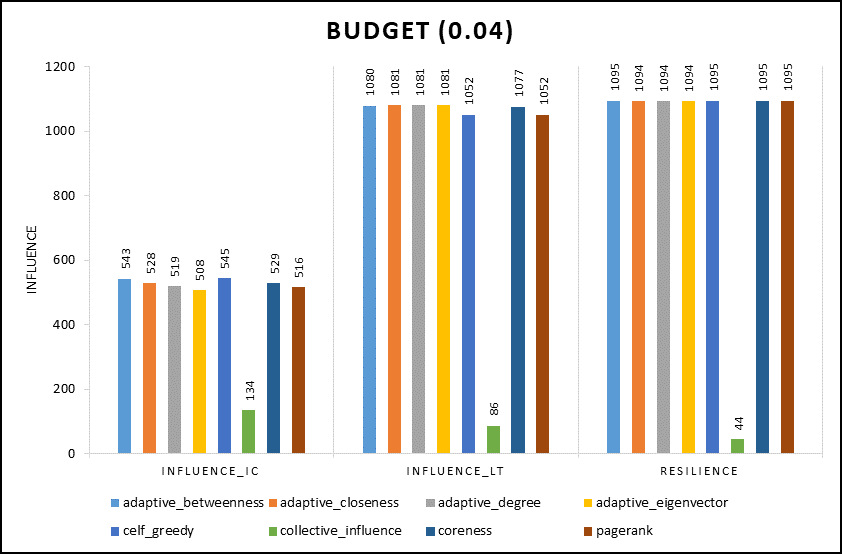
\includegraphics[angle=90, scale=0.65]{automata-budget-4}\par 
				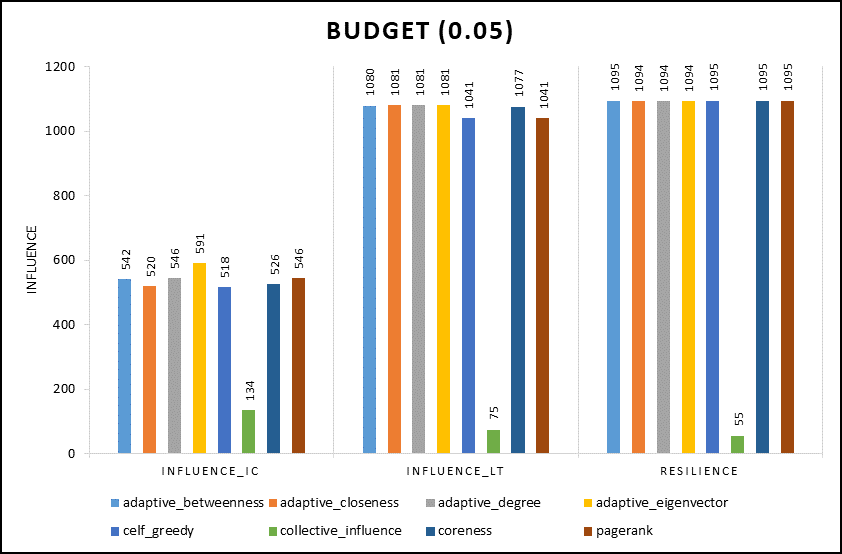
\includegraphics[angle=90, scale=0.65]{automata-budget-5}\par 
			\end{multicols}
			
			\caption{Influence measure of Automata network on range on all budgets evaluated for all three tests.}
			\label{fig:inf-framework-automata}
		\end{figure*}
		
		\begin{figure*}[ht]
			\begin{multicols}{2}
				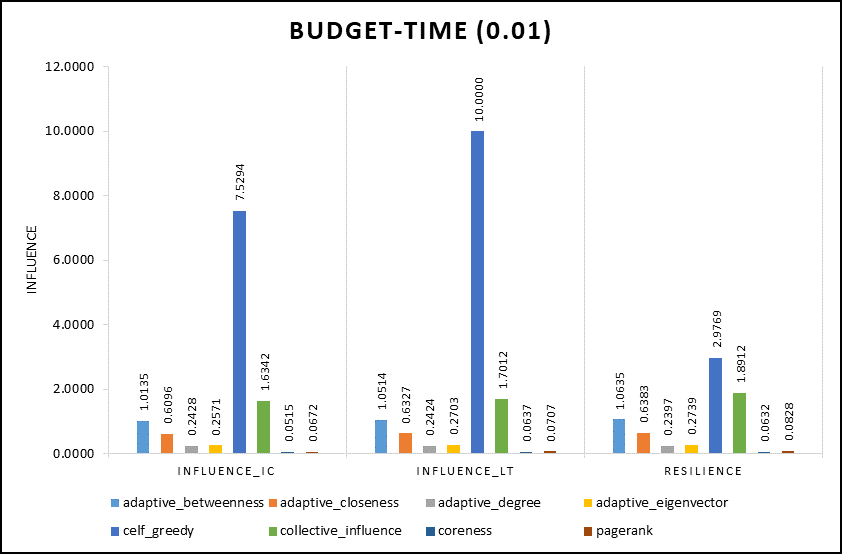
\includegraphics[angle=90, scale=0.65]{automata-budget-time-1}\par 
				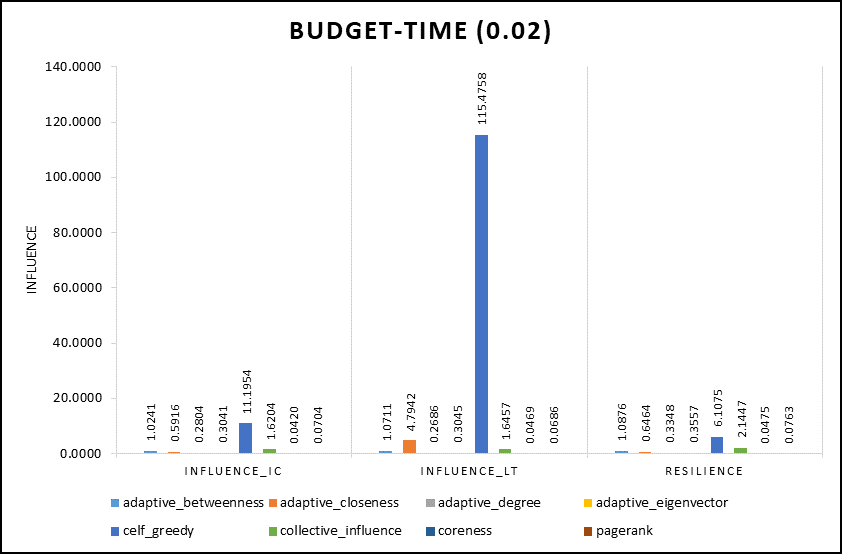
\includegraphics[angle=90, scale=0.65]{automata-budget-time-2}\par 
			\end{multicols}
			\begin{multicols}{2}
				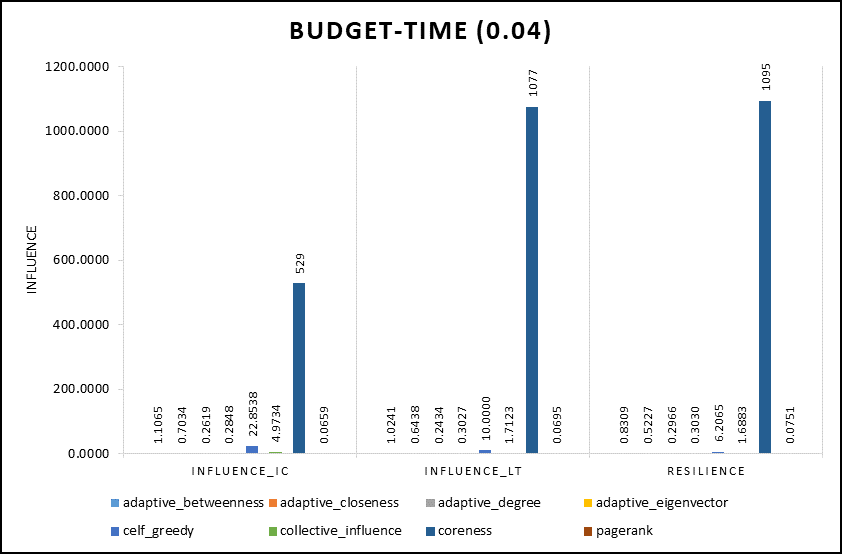
\includegraphics[angle=90, scale=0.65]{automata-budget-time-4}\par 
				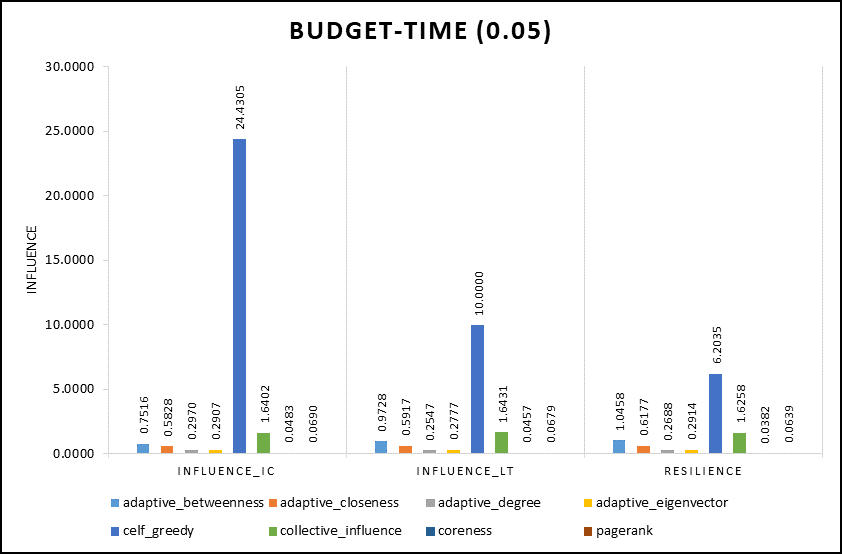
\includegraphics[angle=90, scale=0.65]{automata-budget-time-5}\par 
			\end{multicols}
			
			\caption{Normalized elapsed time for budget criteria on Automata network.}
			\label{fig:inf-framework-automata2}
		\end{figure*}
		
		\begin{figure*}[h]
			\begin{multicols}{2}
				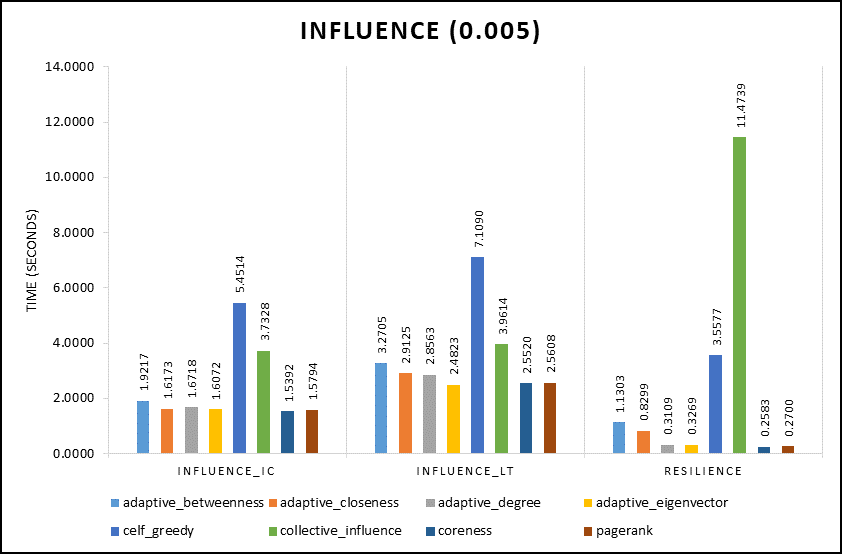
\includegraphics[angle=90, scale=0.65]{automata-influence-1}\par 
				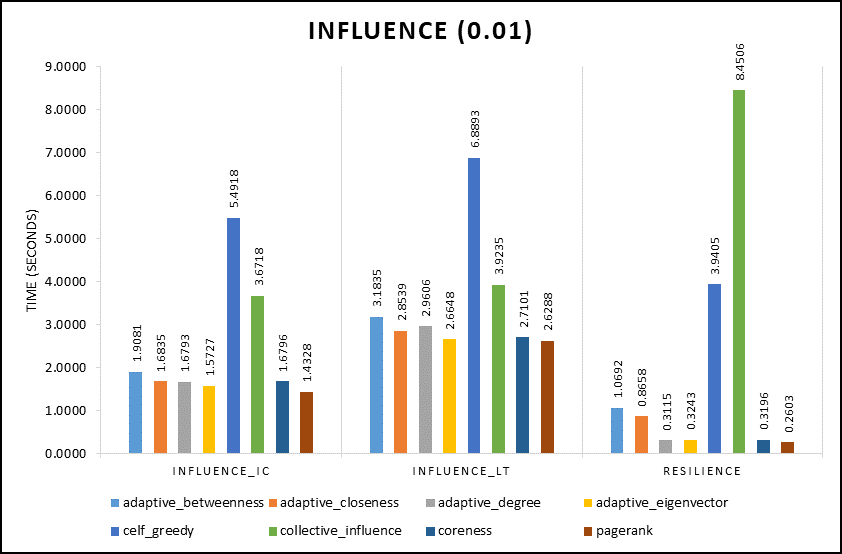
\includegraphics[angle=90, scale=0.65]{automata-influence-2}\par 
			\end{multicols}
			\begin{multicols}{2}
				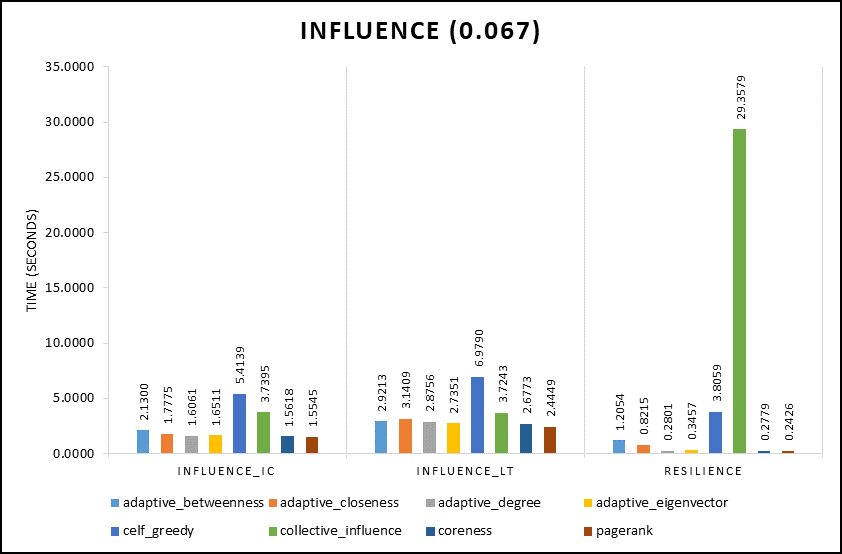
\includegraphics[angle=90, scale=0.65]{automata-influence-4}\par 
				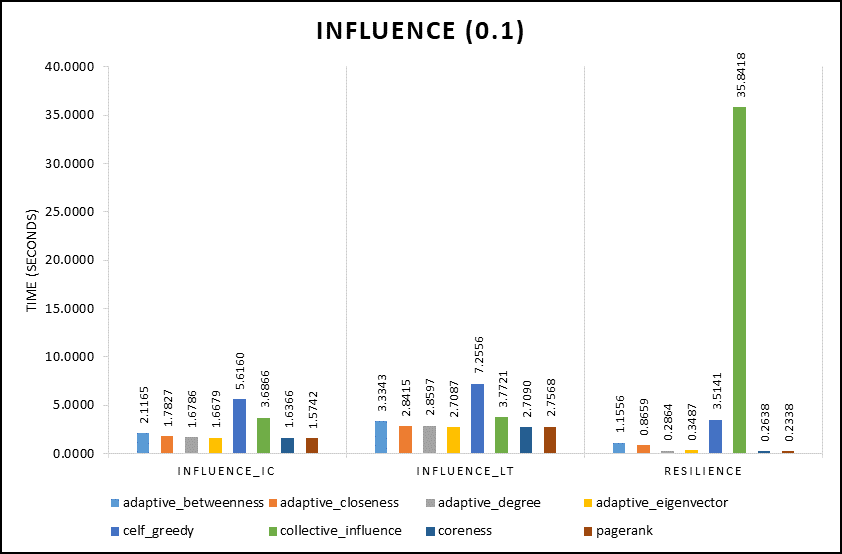
\includegraphics[angle=90, scale=0.65]{automata-influence-5}\par 
			\end{multicols}
			
			\caption{Normalized elapsed time for influence criteria on Automata network.}
			\label{fig:inf-framework-automata3}
		\end{figure*}
		
		
		% *** caida ***
		\begin{figure*}[ht]
			\begin{multicols}{2}
				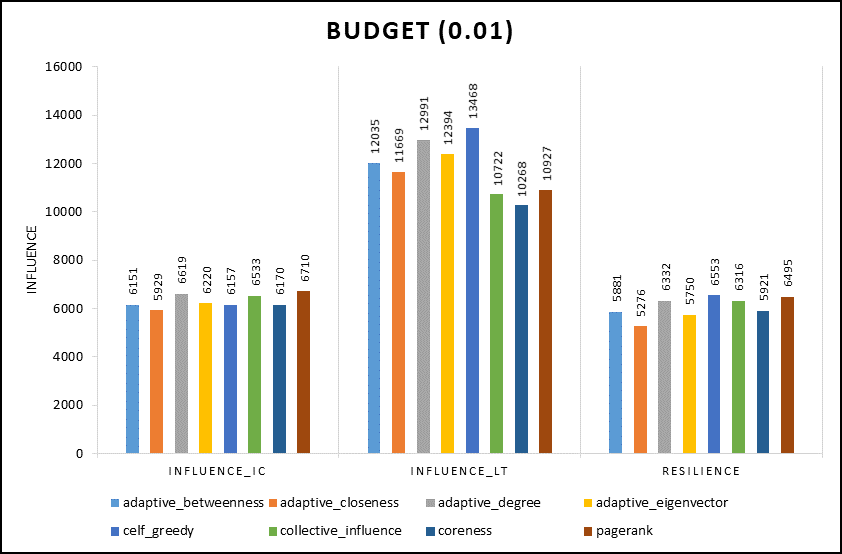
\includegraphics[angle=90, scale=0.65]{caida-budget-1}\par 
				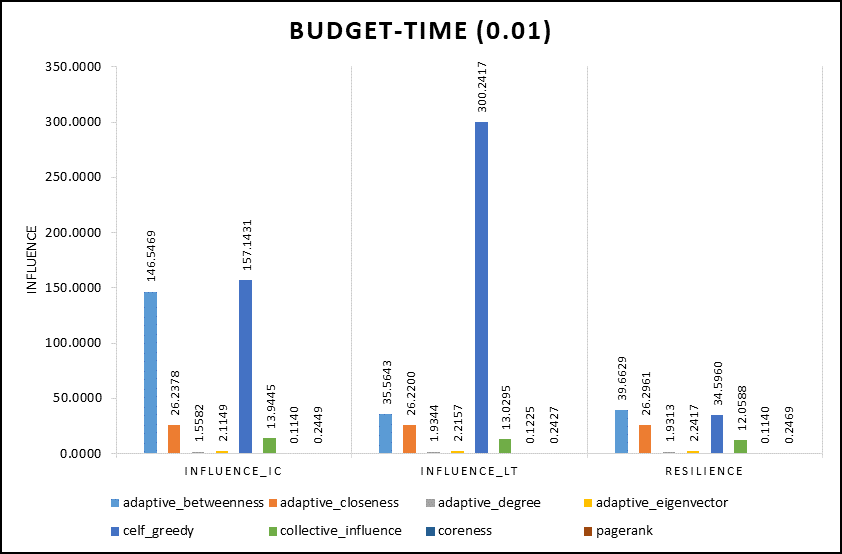
\includegraphics[angle=90, scale=0.65]{caida-budget-time-1}\par 
			\end{multicols}
			\begin{multicols}{2}
				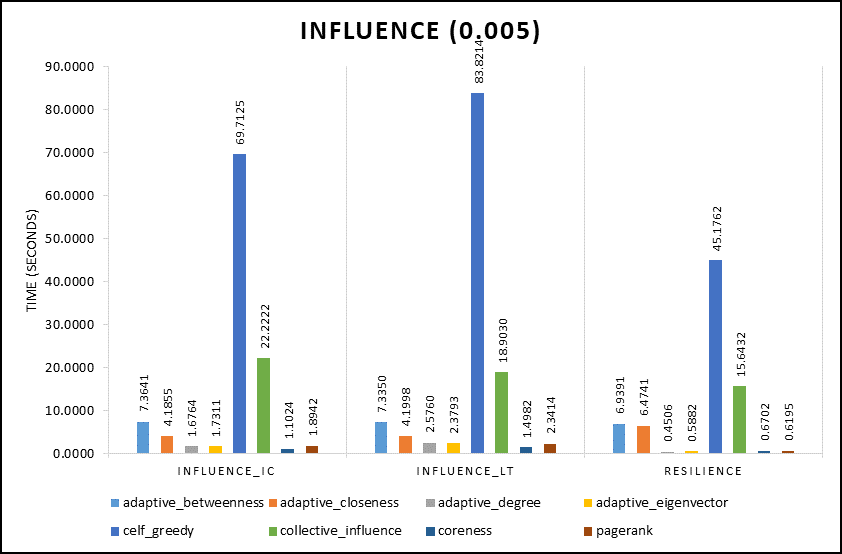
\includegraphics[angle=90, scale=0.65]{caida-influence-1}\par 
			\end{multicols}
			
			\caption{Influence measure (top-left), normalized elapsed time for budget criteria (top-right), and normalized elapsed time for influence criteria (bottom-left) of AS-CAIDA network.}
			\label{fig:inf-framework-caida}
		\end{figure*}
	
		
		% *** city2010 ***
		\begin{figure*}[ht]
			\begin{multicols}{2}
				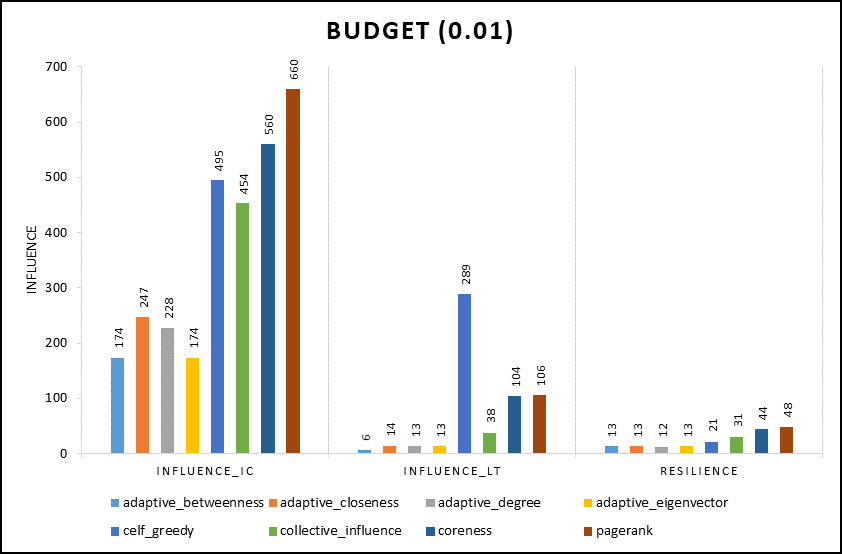
\includegraphics[angle=90, scale=0.65]{city2010-budget-1}\par 
				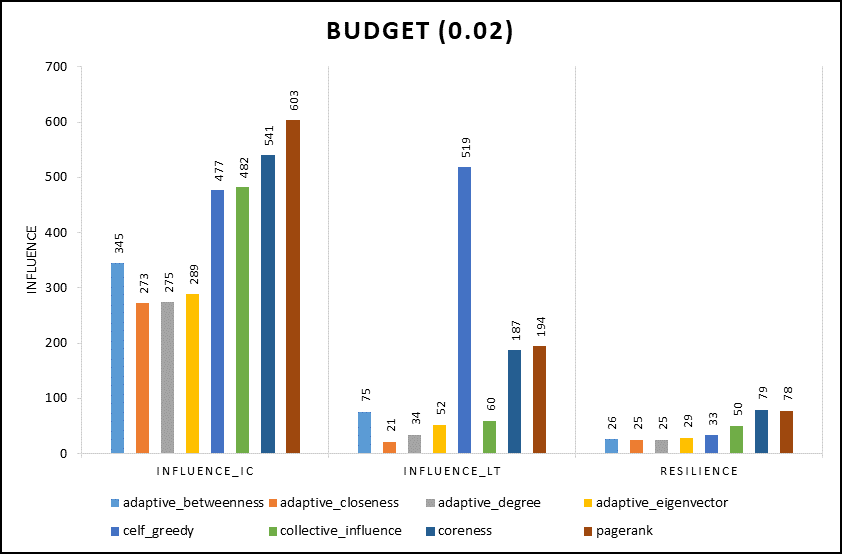
\includegraphics[angle=90, scale=0.65]{city2010-budget-2}\par 
			\end{multicols}
			\begin{multicols}{2}
				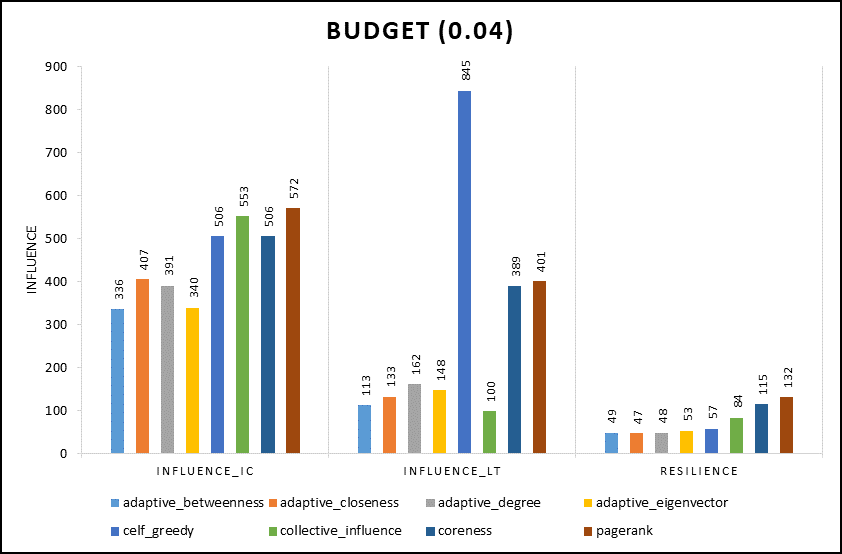
\includegraphics[angle=90, scale=0.65]{city2010-budget-4}\par 
				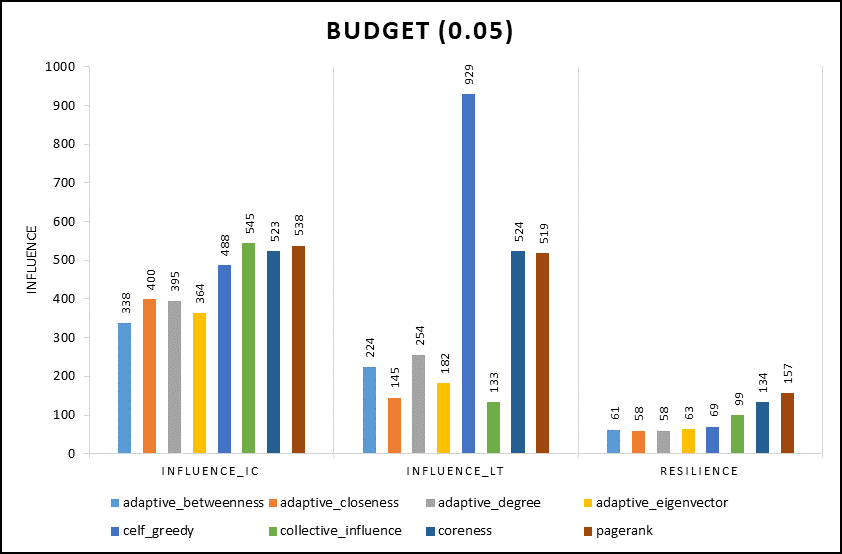
\includegraphics[angle=90, scale=0.65]{city2010-budget-5}\par 
			\end{multicols}
			
			\caption{Influence measure of City network - 2010 on range on all budgets evaluated for all three tests.}
			\label{fig:inf-framework-city2010}
		\end{figure*}
		
		\begin{figure*}[ht]
			\begin{multicols}{2}
				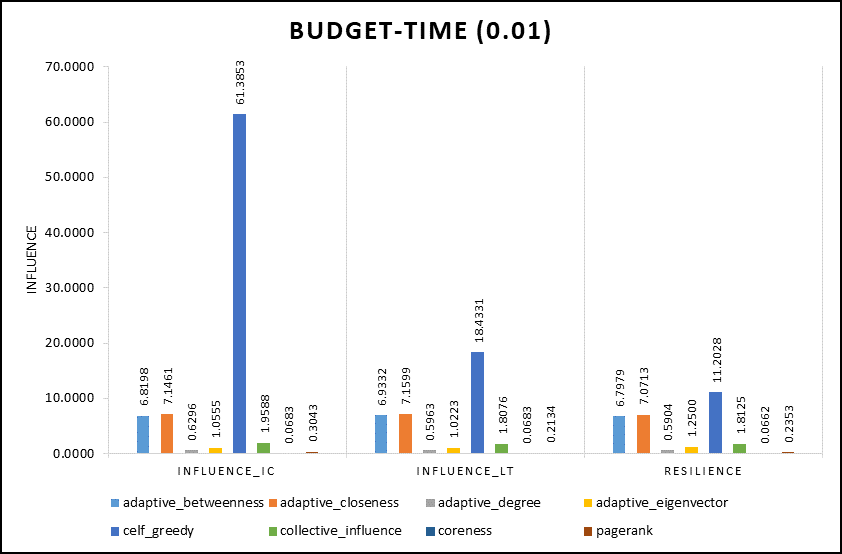
\includegraphics[angle=90, scale=0.65]{city2010-budget-time-1}\par 
				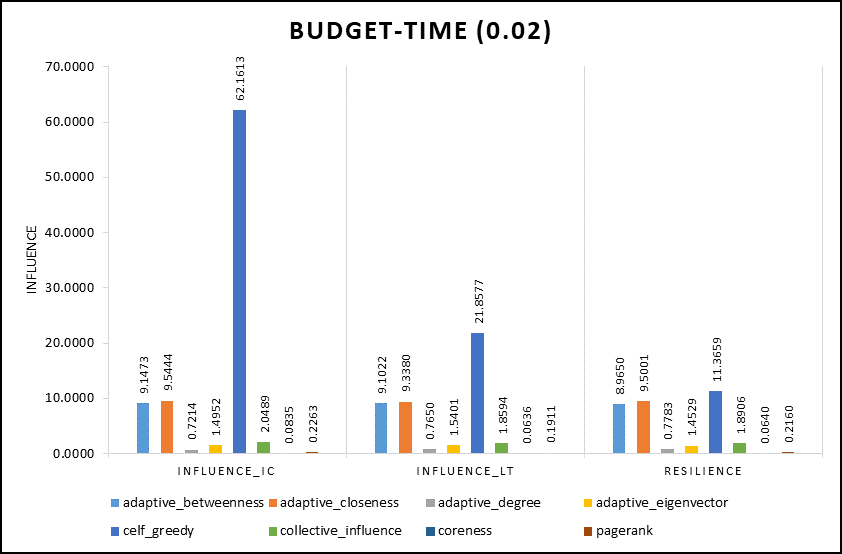
\includegraphics[angle=90, scale=0.65]{city2010-budget-time-2}\par 
			\end{multicols}
			\begin{multicols}{2}
				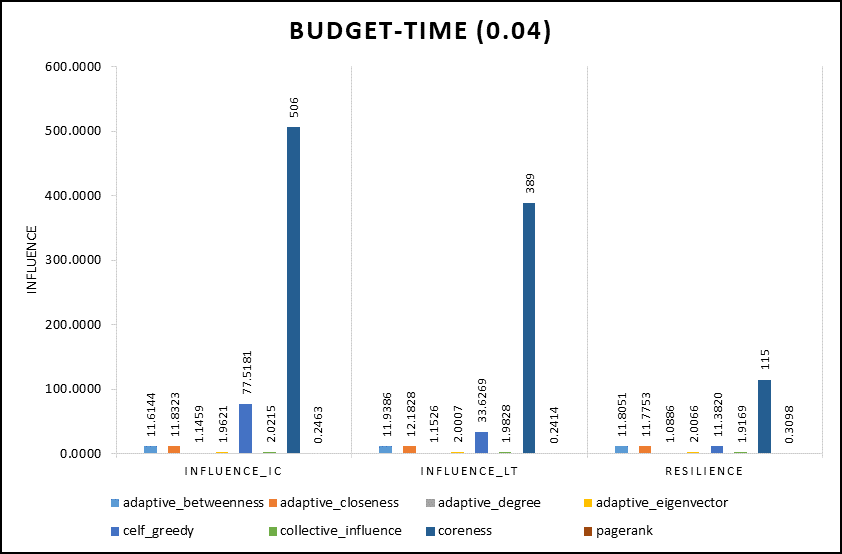
\includegraphics[angle=90, scale=0.65]{city2010-budget-time-4}\par 
				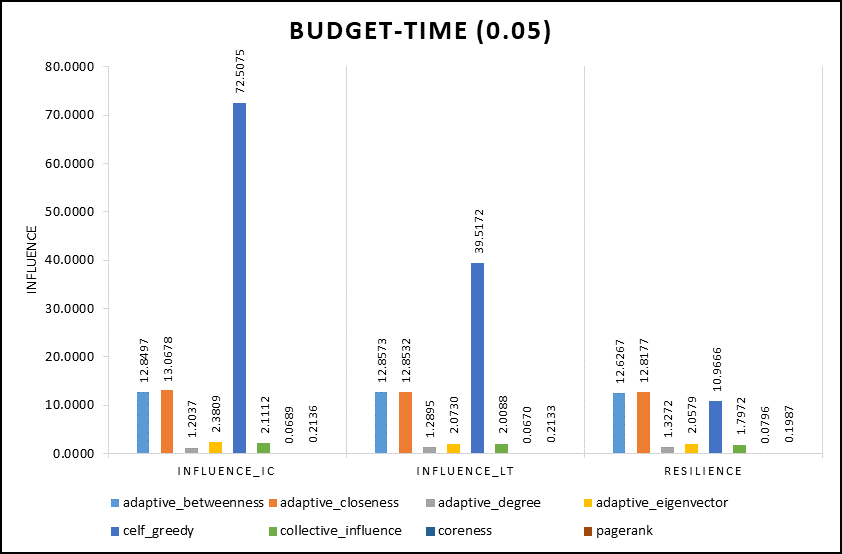
\includegraphics[angle=90, scale=0.65]{city2010-budget-time-5}\par 
			\end{multicols}
			
			\caption{Normalized elapsed time for budget criteria on city2010 network.}
			\label{fig:inf-framework-city2010-2}
		\end{figure*}
		
		\begin{figure*}[h]
			\begin{multicols}{2}
				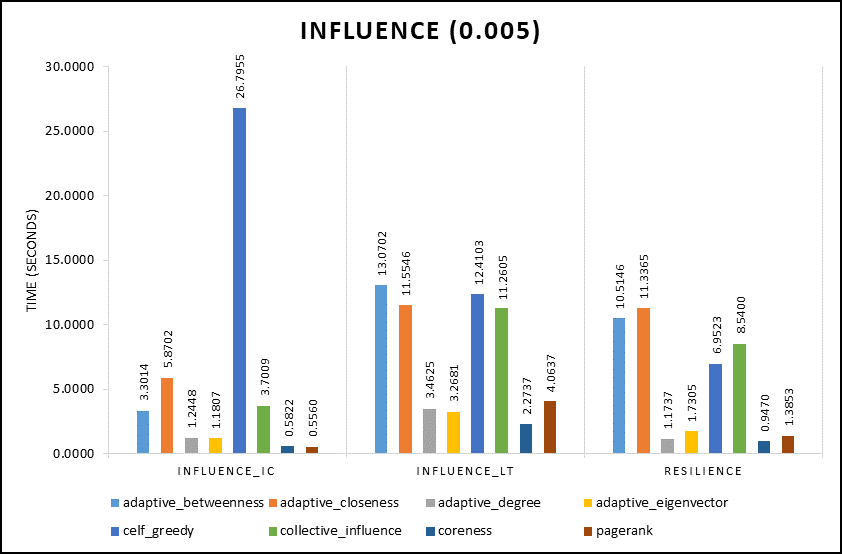
\includegraphics[angle=90, scale=0.65]{city2010-influence-1}\par 
				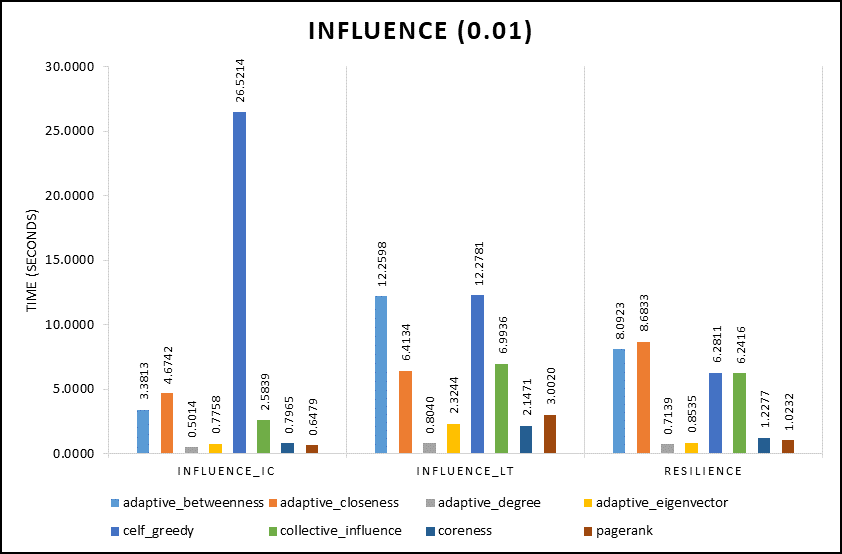
\includegraphics[angle=90, scale=0.65]{city2010-influence-2}\par 
			\end{multicols}
			\begin{multicols}{2}
				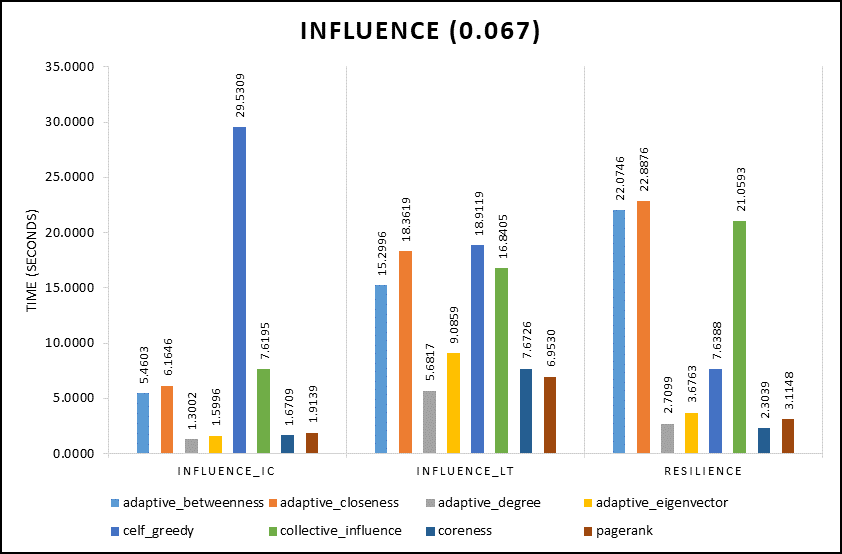
\includegraphics[angle=90, scale=0.65]{city2010-influence-4}\par 
				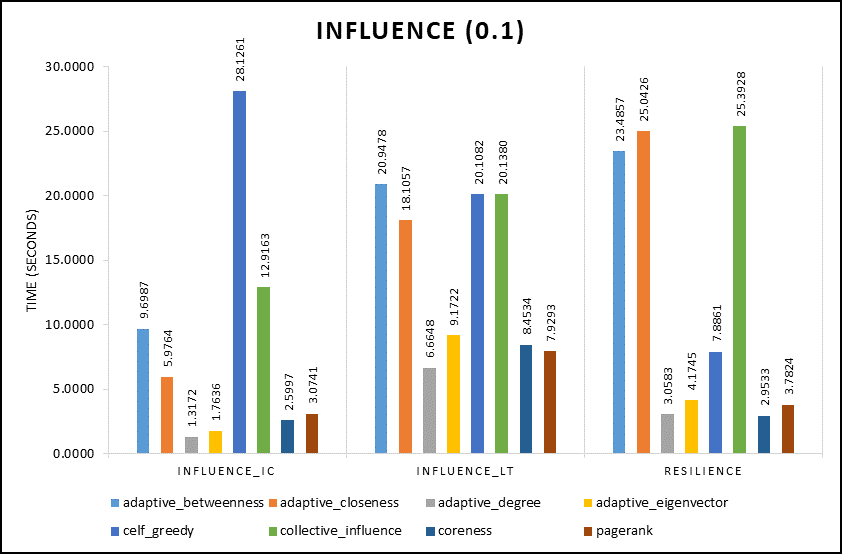
\includegraphics[angle=90, scale=0.65]{city2010-influence-5}\par 
			\end{multicols}
			
			\caption{Normalized elapsed time for influence criteria on City network - 2010.}
			\label{fig:inf-framework-city2010-3}
		\end{figure*}
		
		
		% *** city2013 ***
		\begin{figure*}[ht]
			\begin{multicols}{2}
				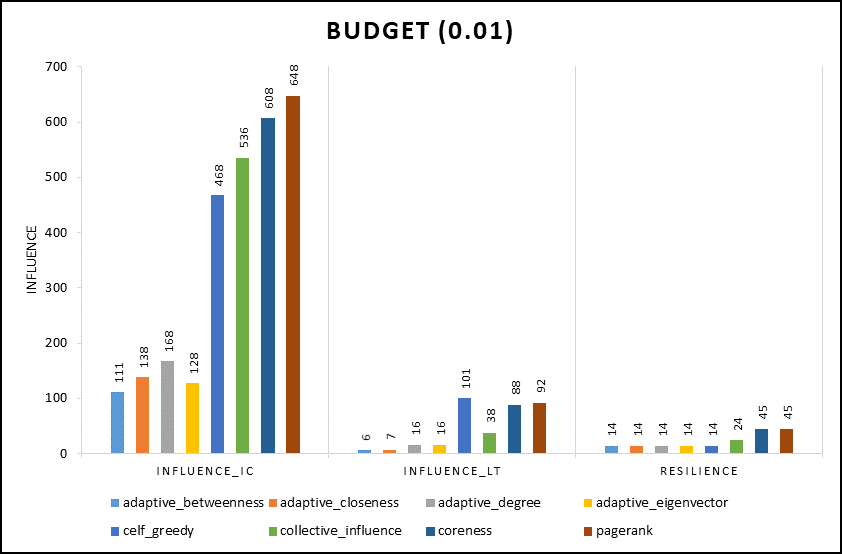
\includegraphics[angle=90, scale=0.65]{city2013-budget-1}\par 
				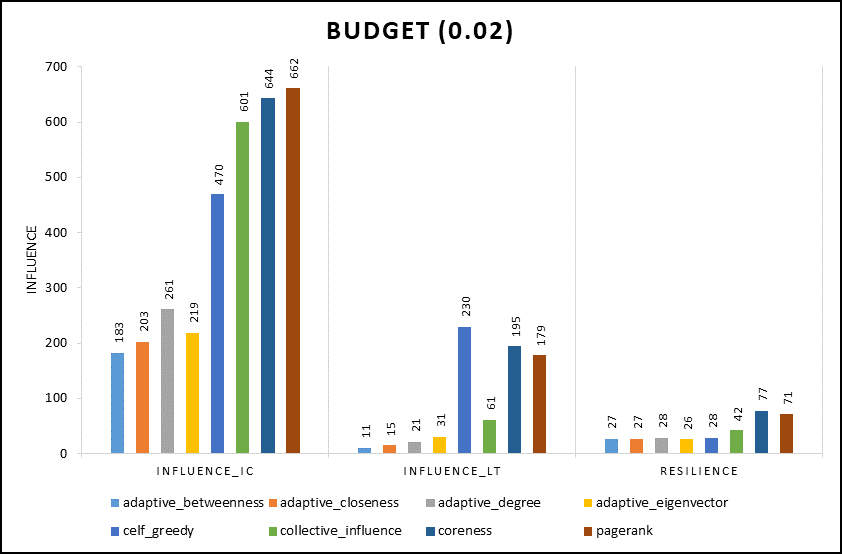
\includegraphics[angle=90, scale=0.65]{city2013-budget-2}\par 
			\end{multicols}
			\begin{multicols}{2}
				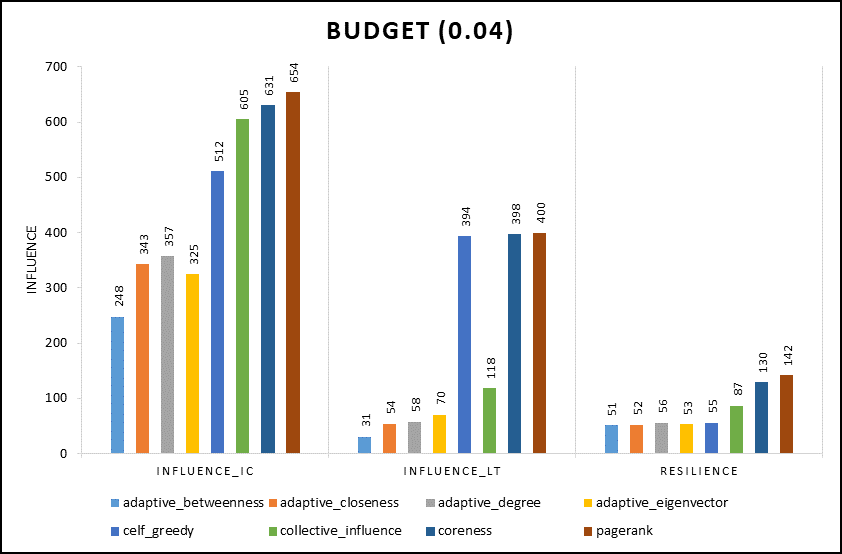
\includegraphics[angle=90, scale=0.65]{city2013-budget-4}\par 
				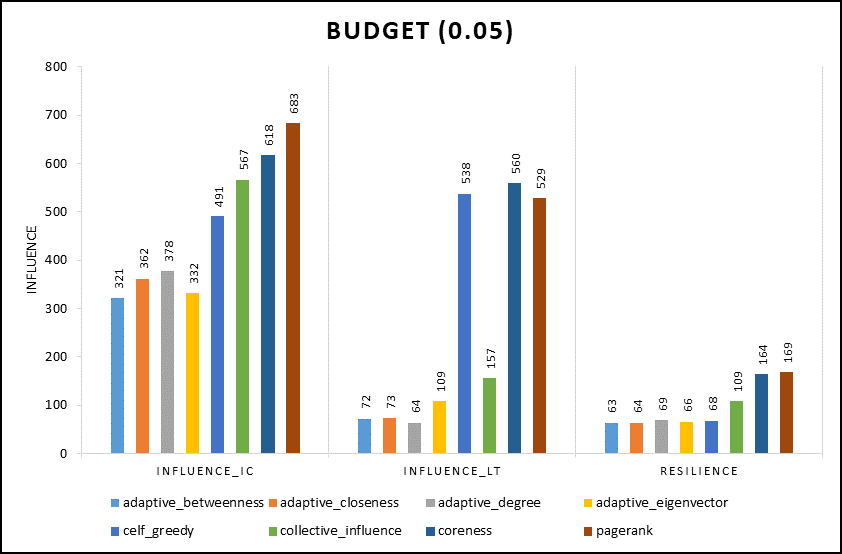
\includegraphics[angle=90, scale=0.65]{city2013-budget-5}\par 
			\end{multicols}
			
			\caption{Influence measure of City network - 2013 on range on all budgets evaluated for all three tests.}
			\label{fig:inf-framework-city2013}
		\end{figure*}
		
		\begin{figure*}[ht]
			\begin{multicols}{2}
				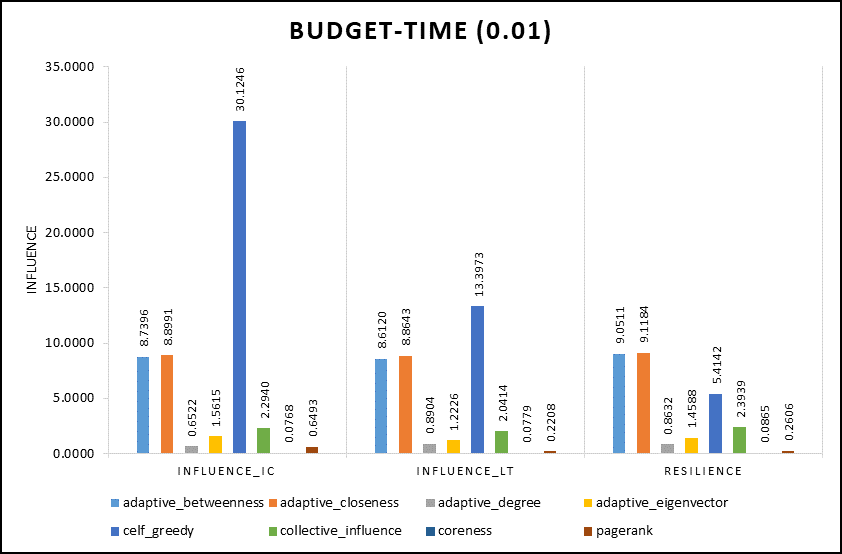
\includegraphics[angle=90, scale=0.65]{city2013-budget-time-1}\par 
				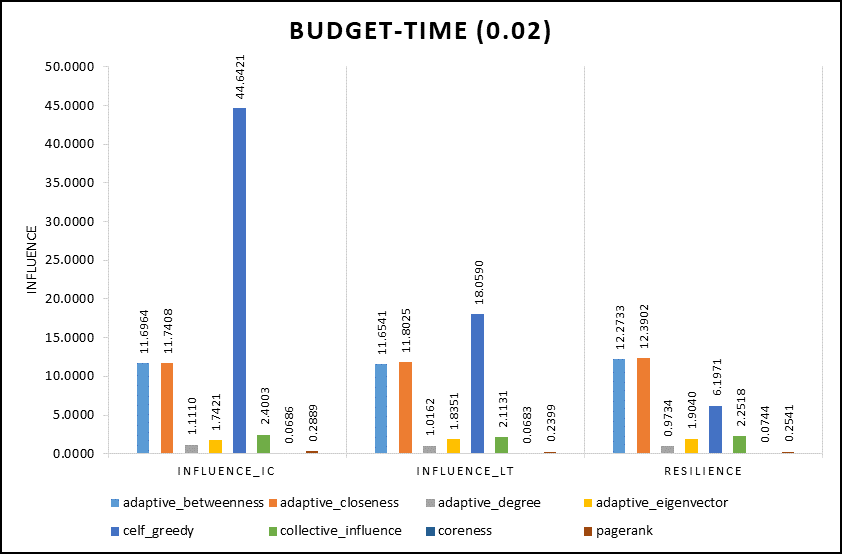
\includegraphics[angle=90, scale=0.65]{city2013-budget-time-2}\par 
			\end{multicols}
			\begin{multicols}{2}
				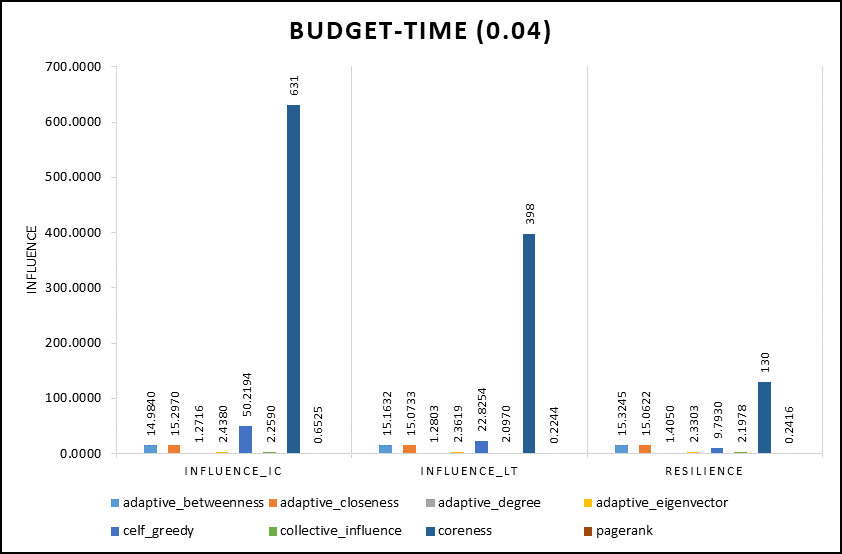
\includegraphics[angle=90, scale=0.65]{city2013-budget-time-4}\par 
				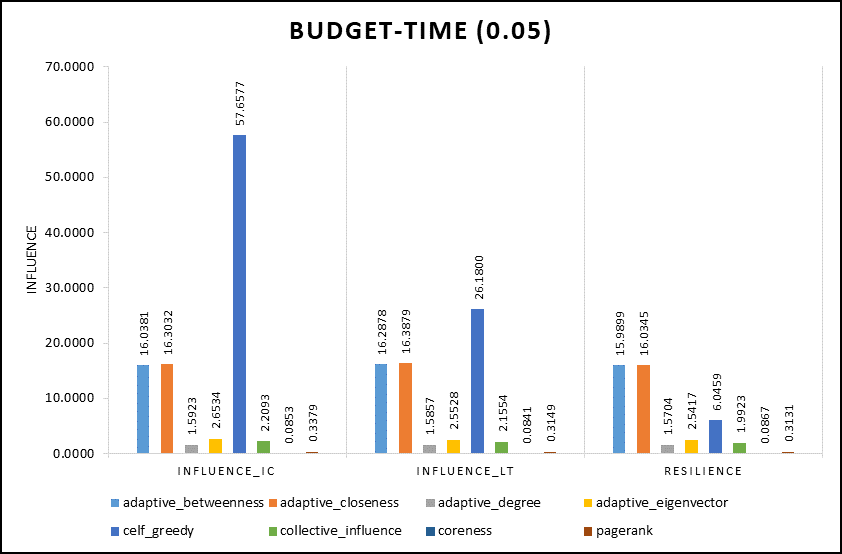
\includegraphics[angle=90, scale=0.65]{city2013-budget-time-5}\par 
			\end{multicols}
			
			\caption{Normalized elapsed time for budget criteria on city2013 network.}
			\label{fig:inf-framework-city2013-2}
		\end{figure*}
		
		\begin{figure*}[h]
			\begin{multicols}{2}
				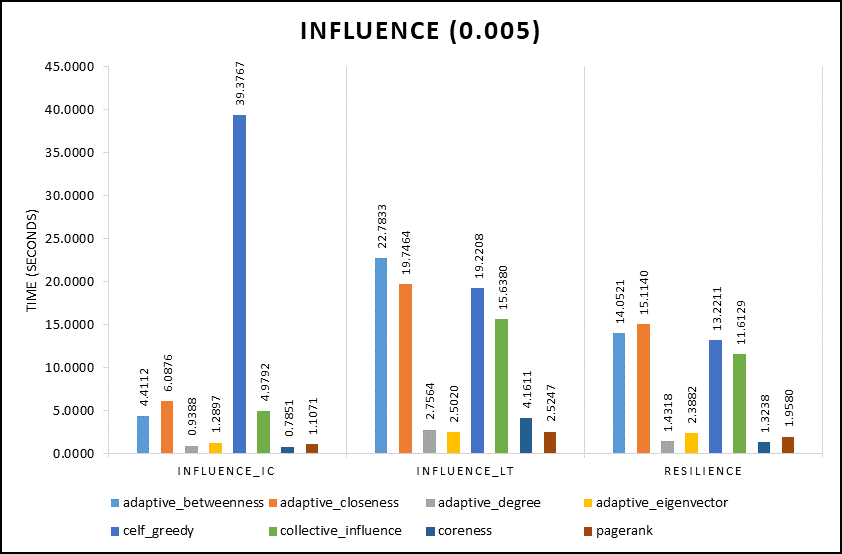
\includegraphics[angle=90, scale=0.65]{city2013-influence-1}\par 
				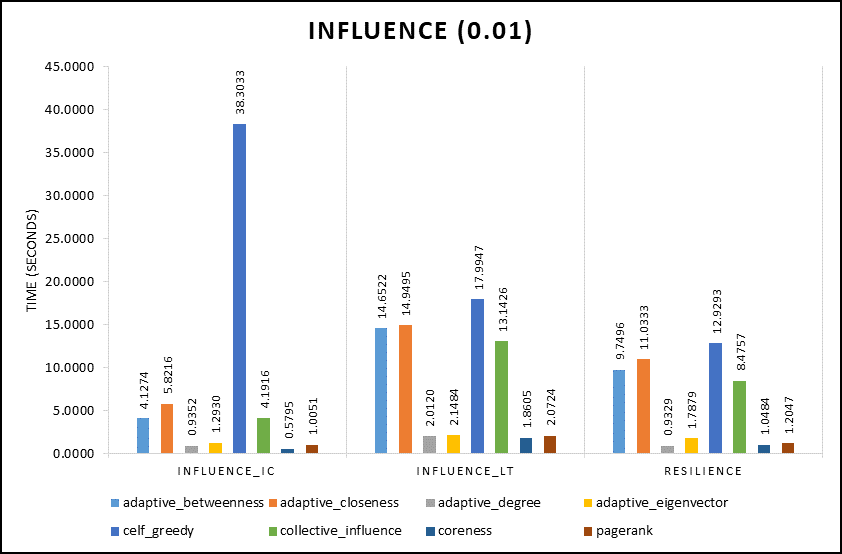
\includegraphics[angle=90, scale=0.65]{city2013-influence-2}\par 
			\end{multicols}
			\begin{multicols}{2}
				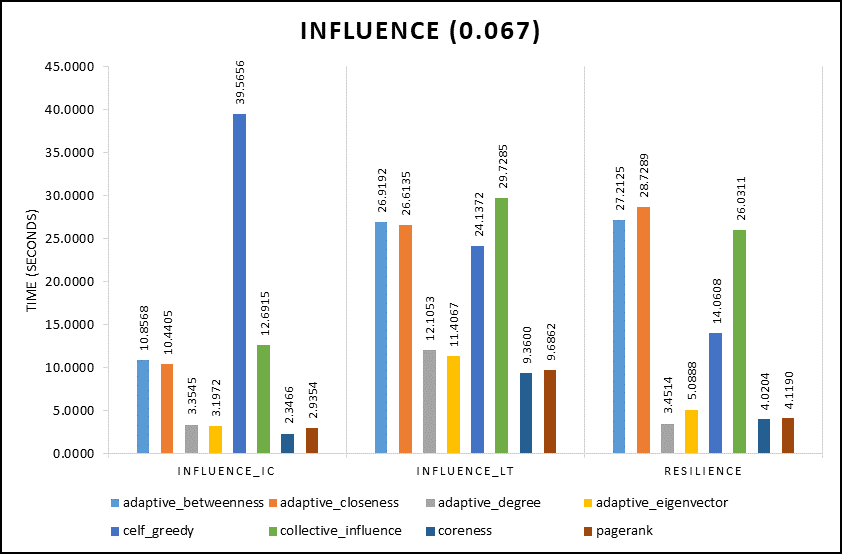
\includegraphics[angle=90, scale=0.65]{city2013-influence-4}\par 
				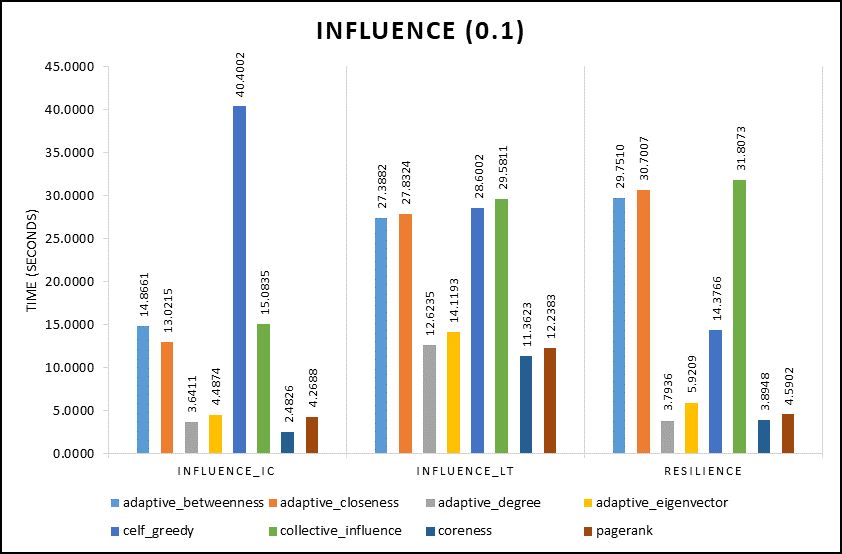
\includegraphics[angle=90, scale=0.65]{city2013-influence-5}\par 
			\end{multicols}
			
			\caption{Normalized elapsed time for influence criteria on City network - 2013.}
			\label{fig:inf-framework-city2013-3}
		\end{figure*}
		
		
		% *** city2016 ***
		\begin{figure*}[ht]
			\begin{multicols}{2}
				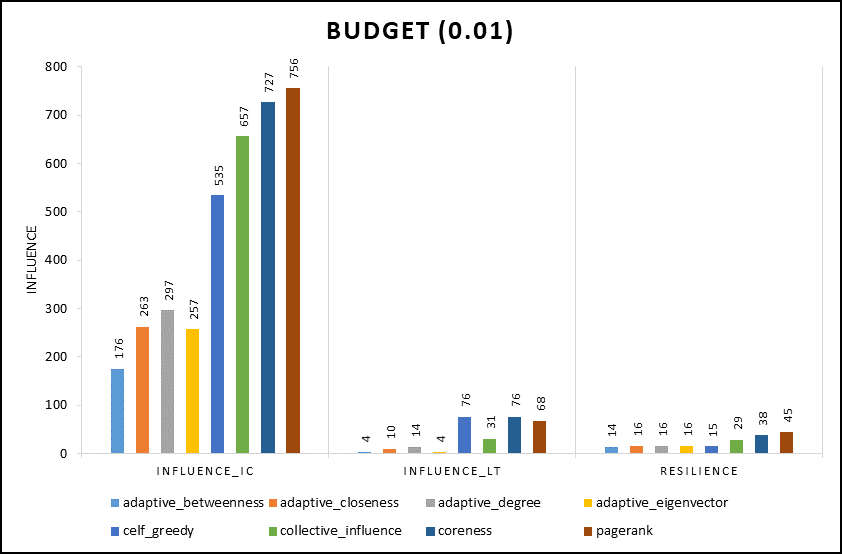
\includegraphics[angle=90, scale=0.65]{city2016-budget-1}\par 
				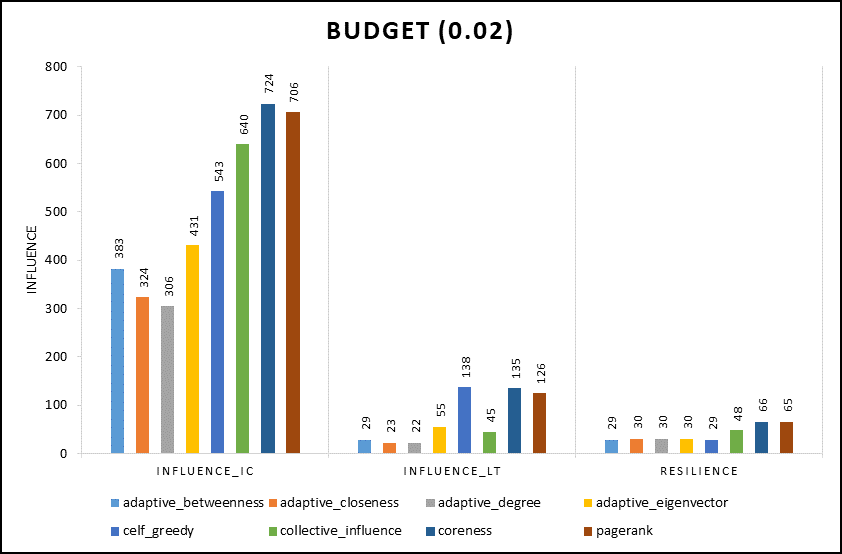
\includegraphics[angle=90, scale=0.65]{city2016-budget-2}\par 
			\end{multicols}
			\begin{multicols}{2}
				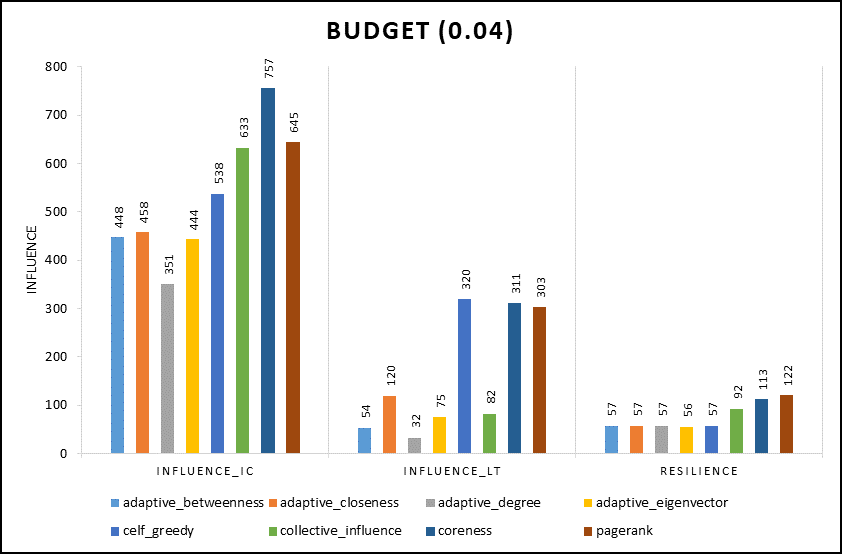
\includegraphics[angle=90, scale=0.65]{city2016-budget-4}\par 
				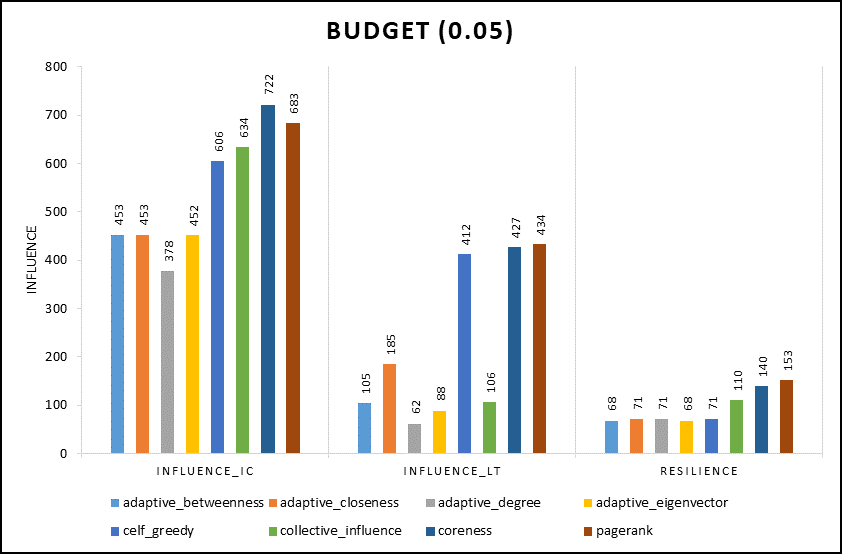
\includegraphics[angle=90, scale=0.65]{city2016-budget-5}\par 
			\end{multicols}
			
			\caption{Influence measure of City network - 2016 on range on all budgets evaluated for all three tests.}
			\label{fig:inf-framework-city2016}
		\end{figure*}
		
		\begin{figure*}[ht]
			\begin{multicols}{2}
				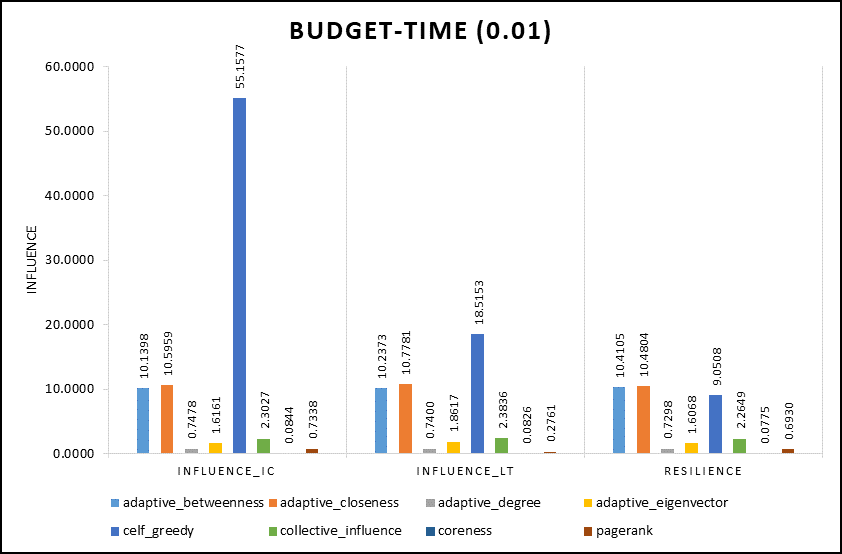
\includegraphics[angle=90, scale=0.65]{city2016-budget-time-1}\par 
				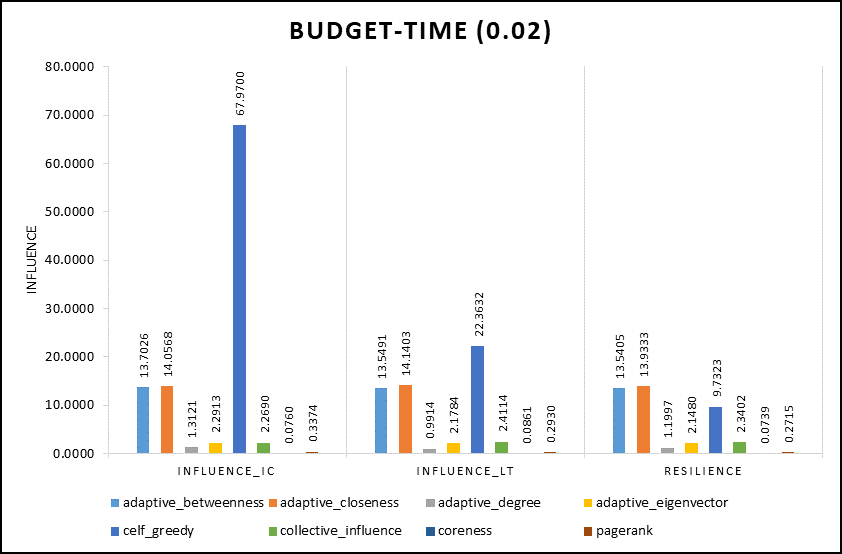
\includegraphics[angle=90, scale=0.65]{city2016-budget-time-2}\par 
			\end{multicols}
			\begin{multicols}{2}
				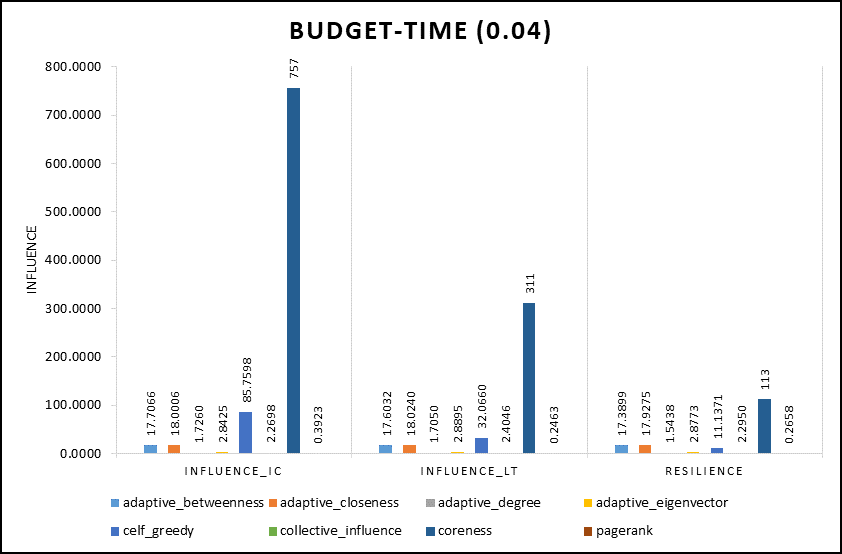
\includegraphics[angle=90, scale=0.65]{city2016-budget-time-4}\par 
				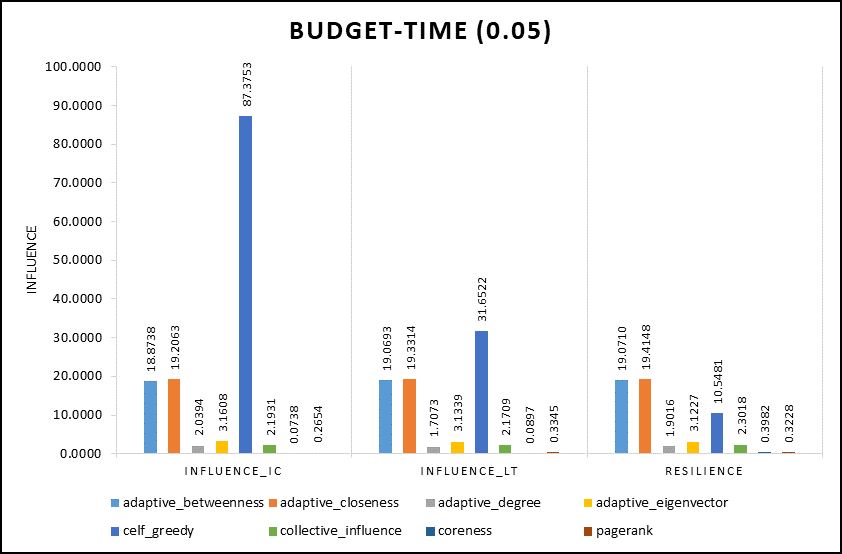
\includegraphics[angle=90, scale=0.65]{city2016-budget-time-5}\par 
			\end{multicols}
			
			\caption{Normalized elapsed time for budget criteria on city2016 network.}
			\label{fig:inf-framework-city2016-2}
		\end{figure*}
		
		\begin{figure*}[h]
			\begin{multicols}{2}
				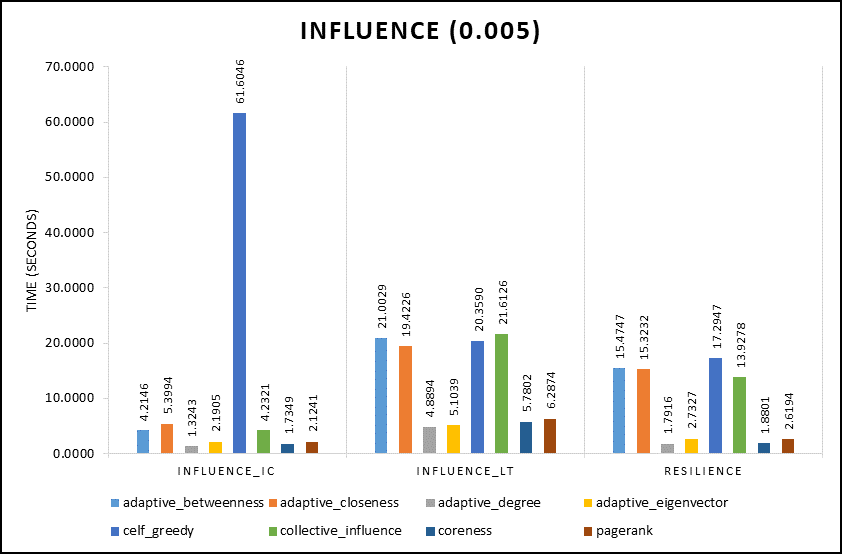
\includegraphics[angle=90, scale=0.65]{city2016-influence-1}\par 
				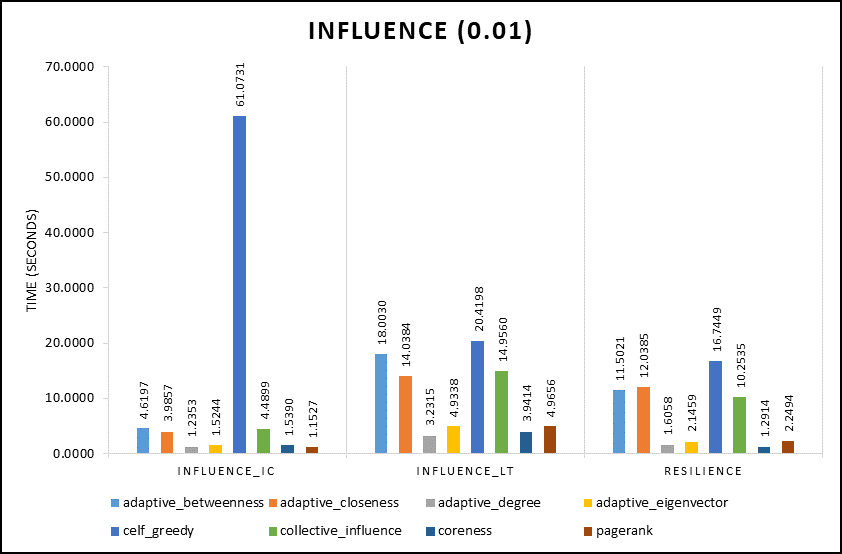
\includegraphics[angle=90, scale=0.65]{city2016-influence-2}\par 
			\end{multicols}
			\begin{multicols}{2}
				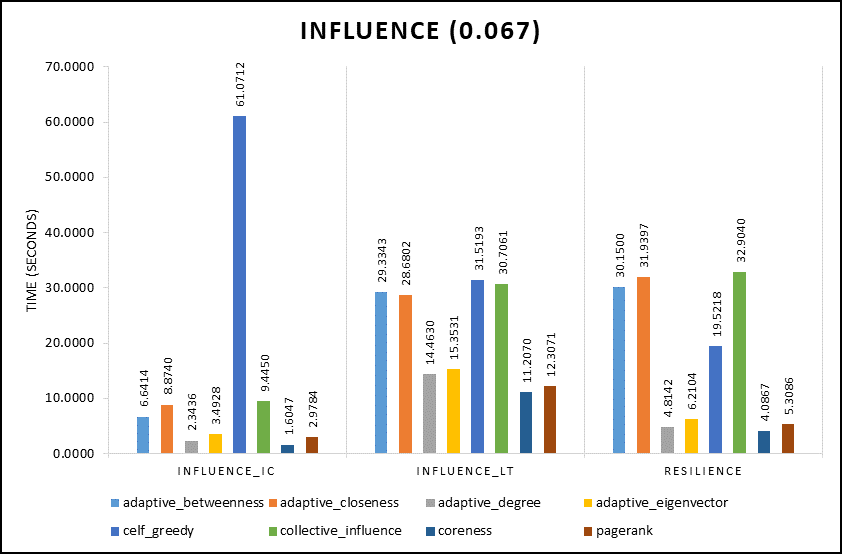
\includegraphics[angle=90, scale=0.65]{city2016-influence-4}\par 
				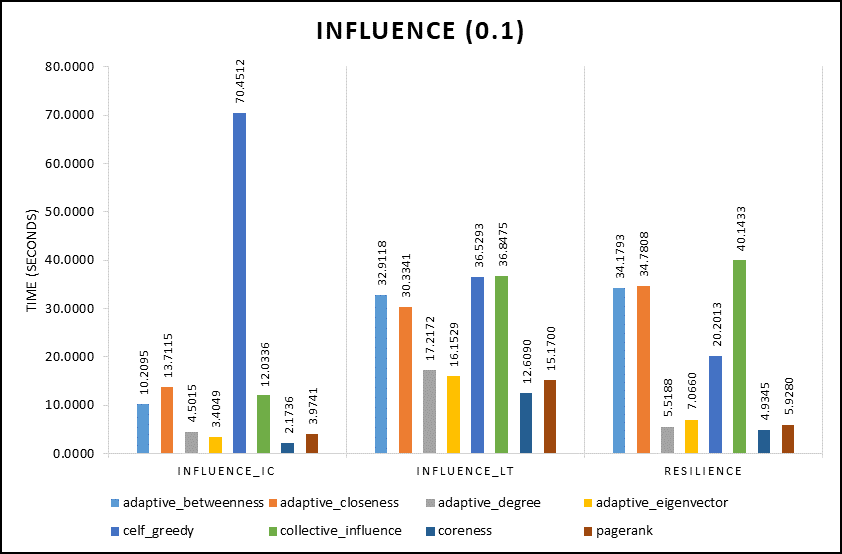
\includegraphics[angle=90, scale=0.65]{city2016-influence-5}\par 
			\end{multicols}
			
			\caption{Normalized elapsed time for influence criteria on City network - 2016.}
			\label{fig:inf-framework-city2016-3}
		\end{figure*}
		
		
		% *** city2019 ***
		\begin{figure*}[ht]
			\begin{multicols}{2}
				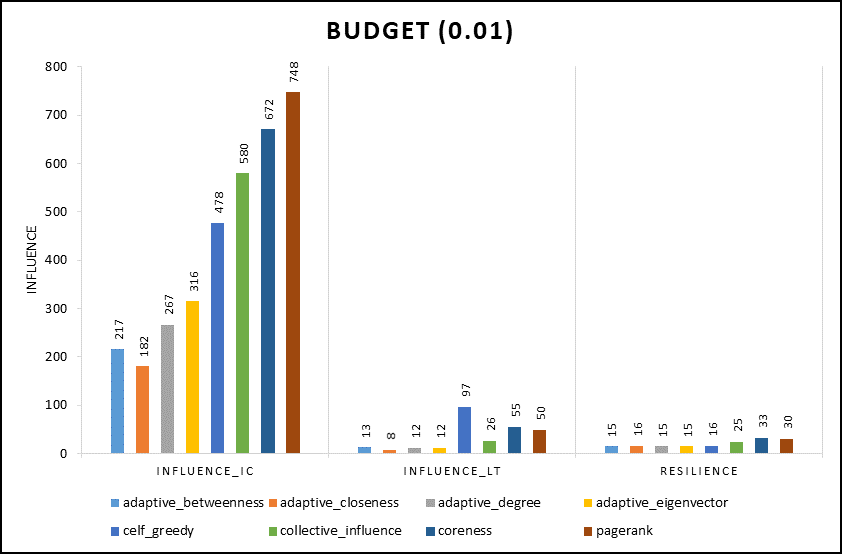
\includegraphics[angle=90, scale=0.65]{city2019-budget-1}\par 
				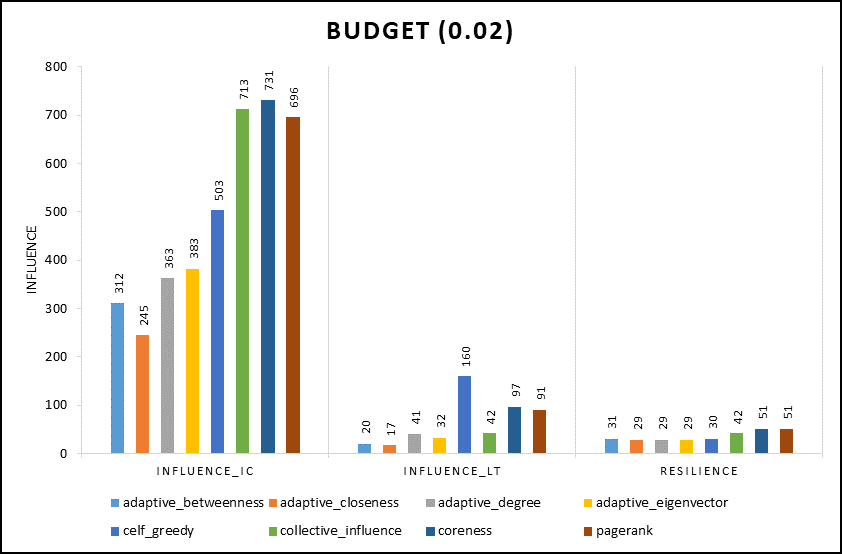
\includegraphics[angle=90, scale=0.65]{city2019-budget-2}\par 
			\end{multicols}
			\begin{multicols}{2}
				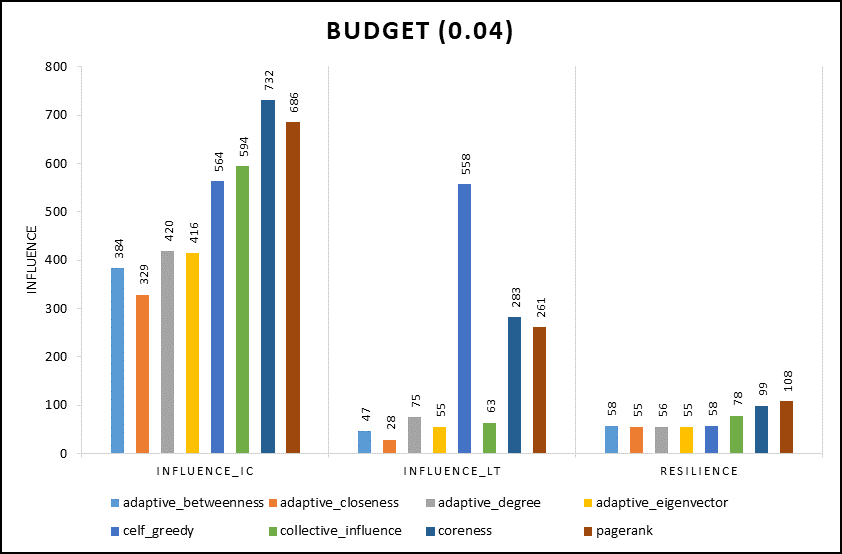
\includegraphics[angle=90, scale=0.65]{city2019-budget-4}\par 
				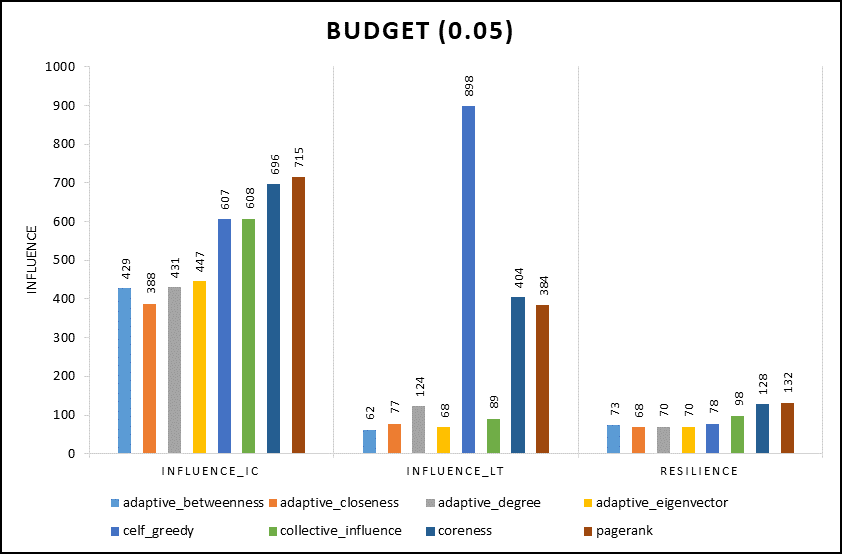
\includegraphics[angle=90, scale=0.65]{city2019-budget-5}\par 
			\end{multicols}
			
			\caption{Influence measure of City network - 2019 on range on all budgets evaluated for all three tests.}
			\label{fig:inf-framework-city2019}
		\end{figure*}
		
		\begin{figure*}[ht]
			\begin{multicols}{2}
				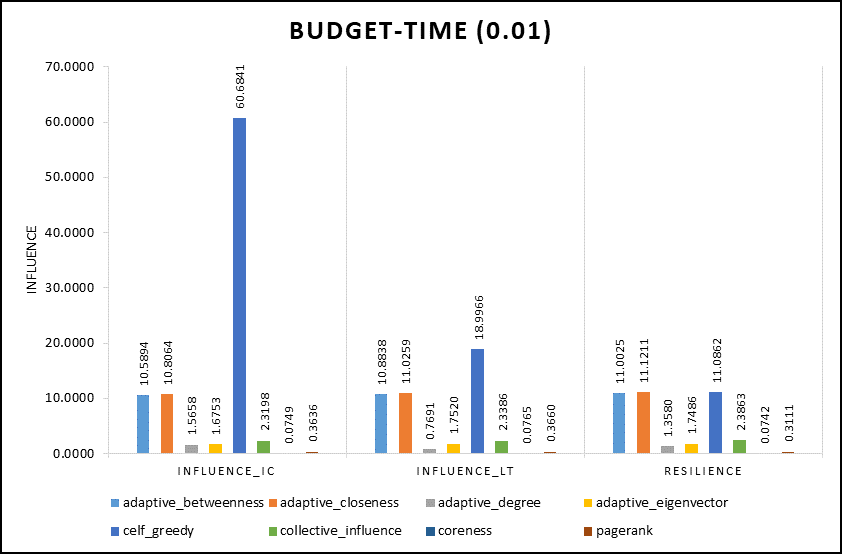
\includegraphics[angle=90, scale=0.65]{city2019-budget-time-1}\par 
				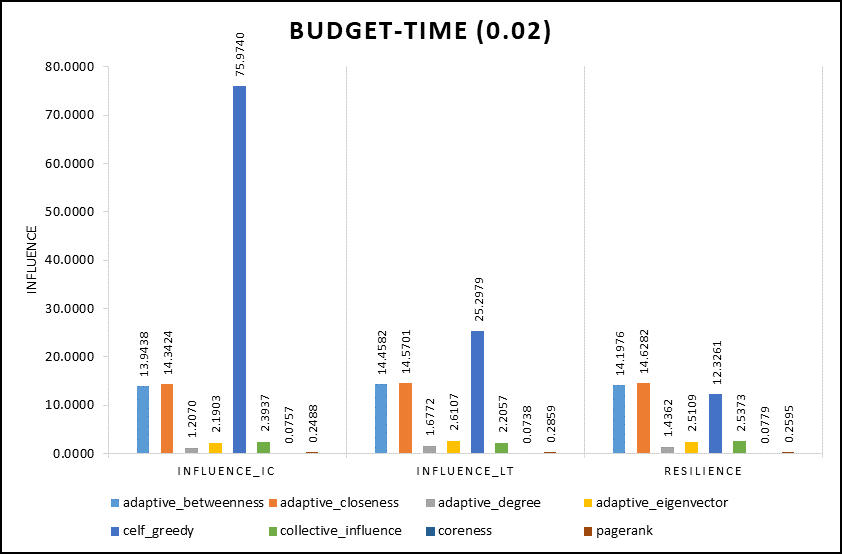
\includegraphics[angle=90, scale=0.65]{city2019-budget-time-2}\par 
			\end{multicols}
			\begin{multicols}{2}
				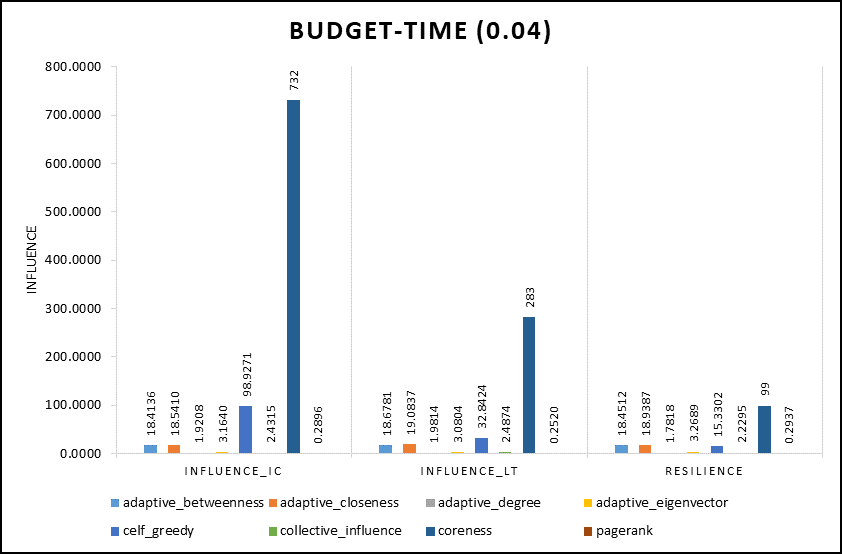
\includegraphics[angle=90, scale=0.65]{city2019-budget-time-4}\par 
				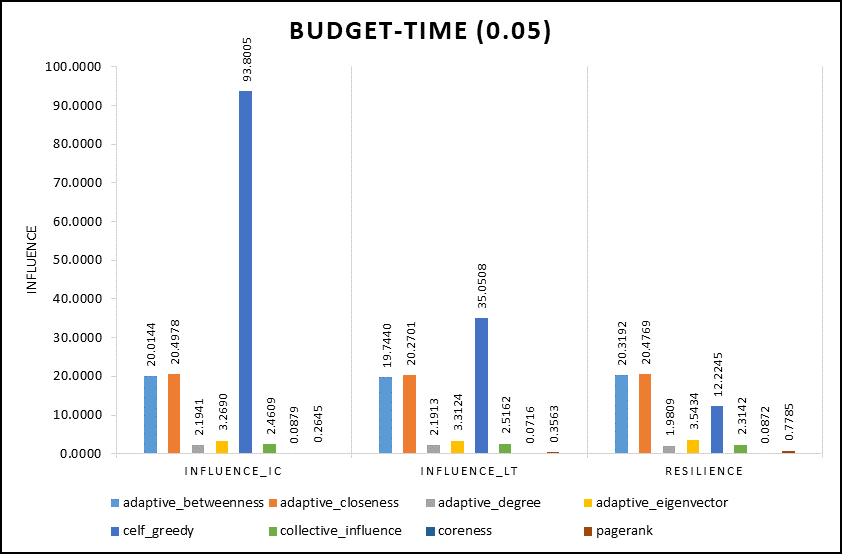
\includegraphics[angle=90, scale=0.65]{city2019-budget-time-5}\par 
			\end{multicols}
			
			\caption{Normalized elapsed time for budget criteria on city2019 network.}
			\label{fig:inf-framework-city2019-2}
		\end{figure*}
		
		\begin{figure*}[h]
			\begin{multicols}{2}
				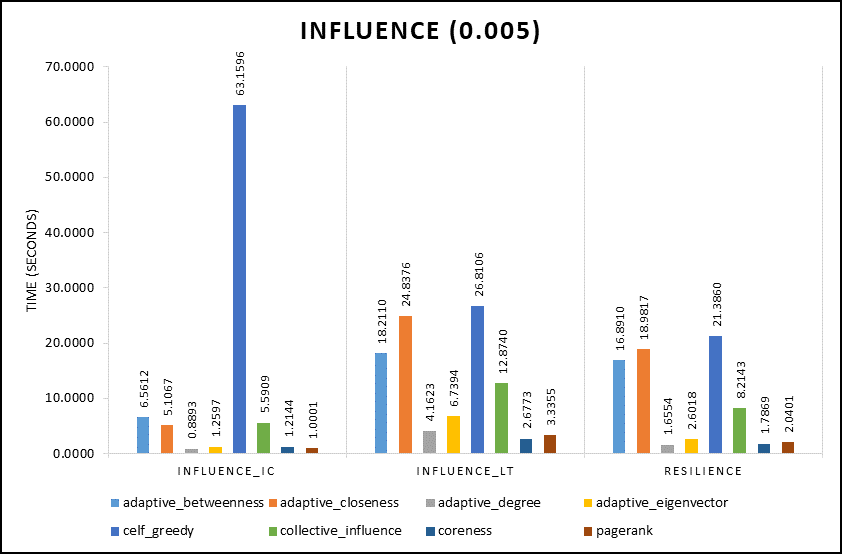
\includegraphics[angle=90, scale=0.65]{city2019-influence-1}\par 
				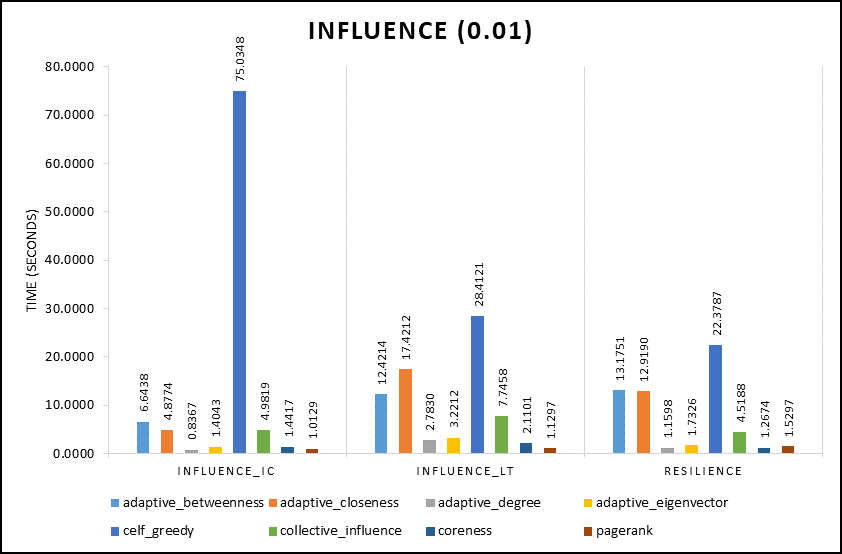
\includegraphics[angle=90, scale=0.65]{city2019-influence-2}\par 
			\end{multicols}
			\begin{multicols}{2}
				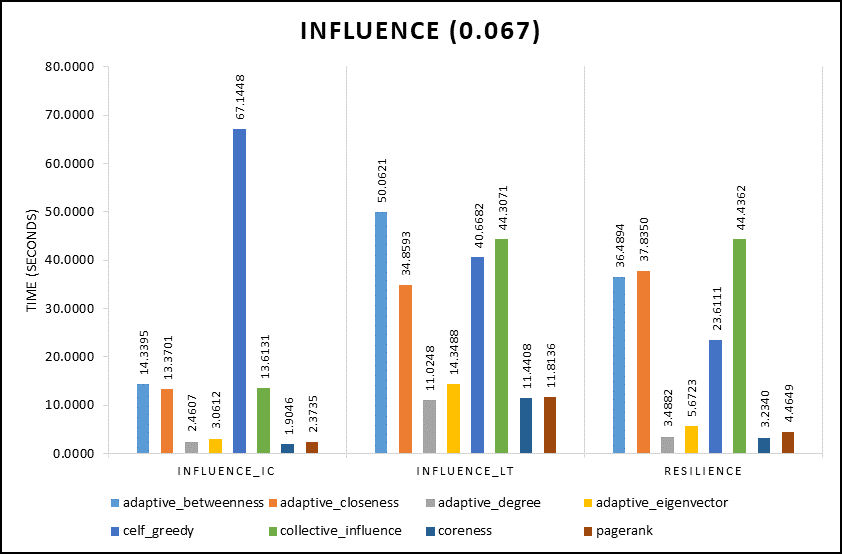
\includegraphics[angle=90, scale=0.65]{city2019-influence-4}\par 
				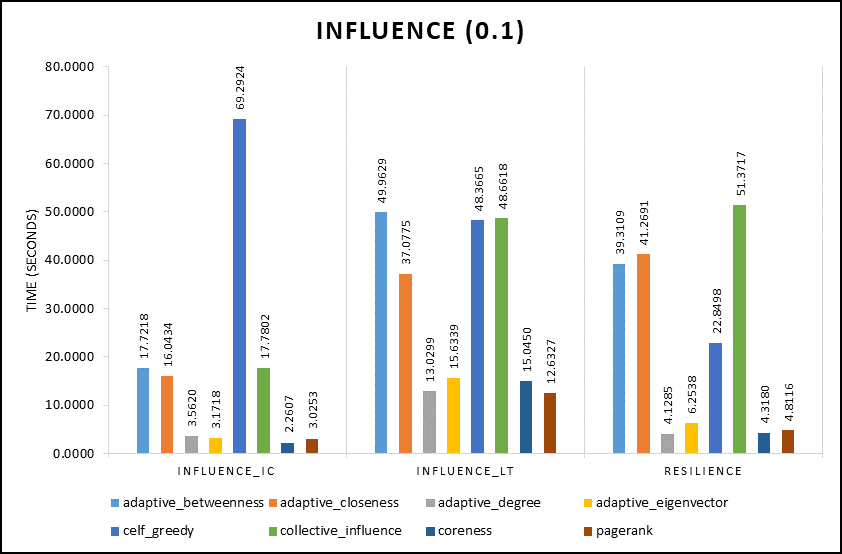
\includegraphics[angle=90, scale=0.65]{city2019-influence-5}\par 
			\end{multicols}
			
			\caption{Normalized elapsed time for influence criteria on City network - 2019.}
			\label{fig:inf-framework-city2019-3}
		\end{figure*}
		
		
		% *** fb_johnshopkins ***
		\begin{figure*}[ht]
			\begin{multicols}{2}
				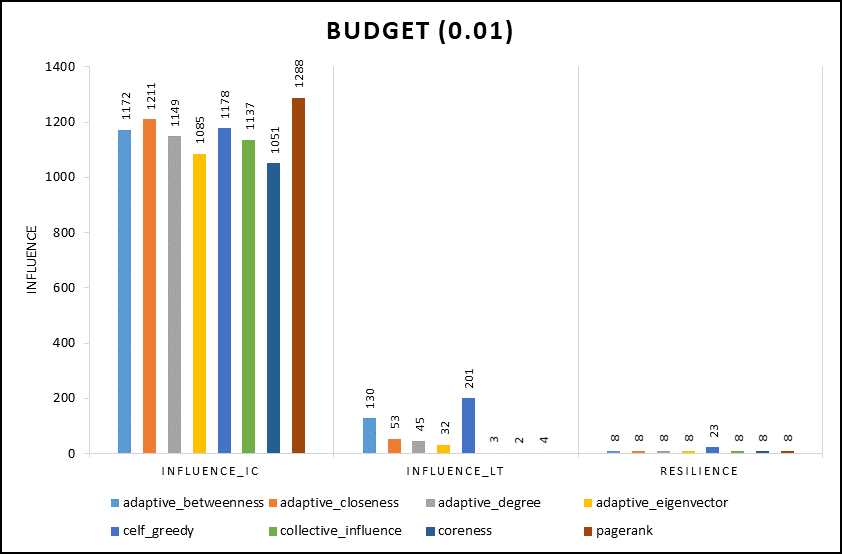
\includegraphics[angle=90, scale=0.65]{fb_johnshopkins-budget-1}\par 
				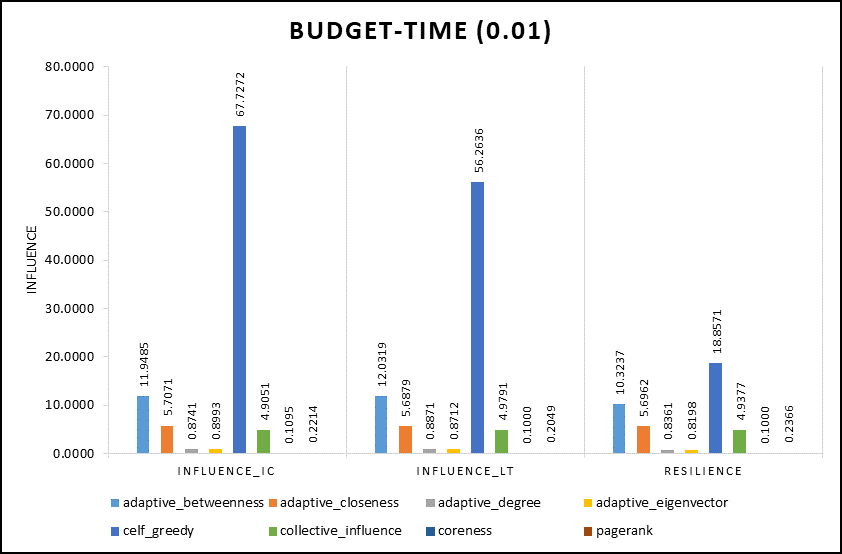
\includegraphics[angle=90, scale=0.65]{fb_johnshopkins-budget-time-1}\par 
			\end{multicols}
			\begin{multicols}{2}
				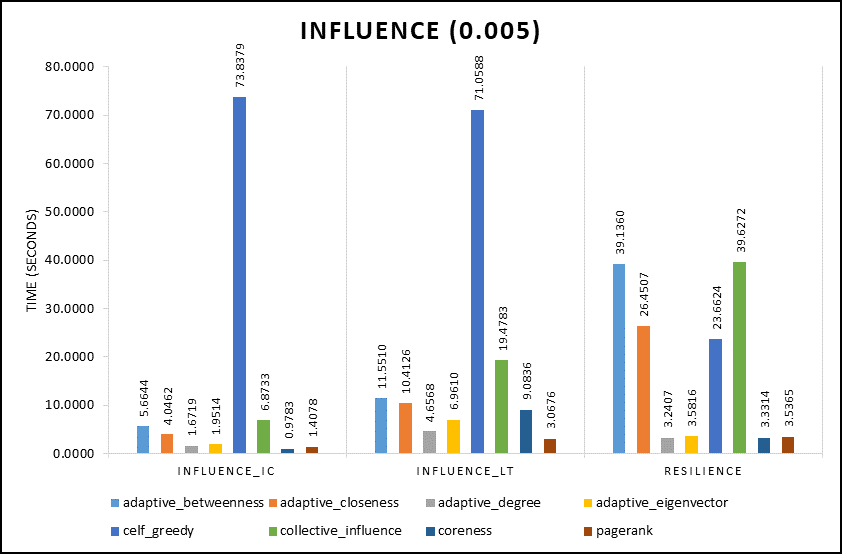
\includegraphics[angle=90, scale=0.65]{fb_johnshopkins-influence-1}\par 
			\end{multicols}
			
			\caption{Influence measure (top-left), normalized elapsed time for budget criteria (top-right), and normalized elapsed time for influence criteria (bottom-left) of Facebook - Johns Hopkins network.}
			\label{fig:inf-framework-fb_johnshopkins}
		\end{figure*}
		
		
		% *** fb_tvshows ***
		\begin{figure*}[ht]
			\begin{multicols}{2}
				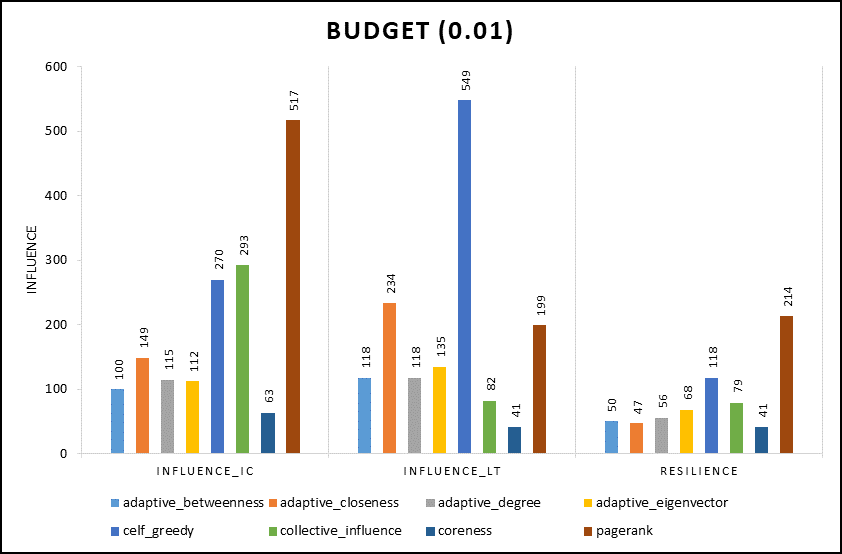
\includegraphics[angle=90, scale=0.65]{fb_tvshows-budget-1}\par 
				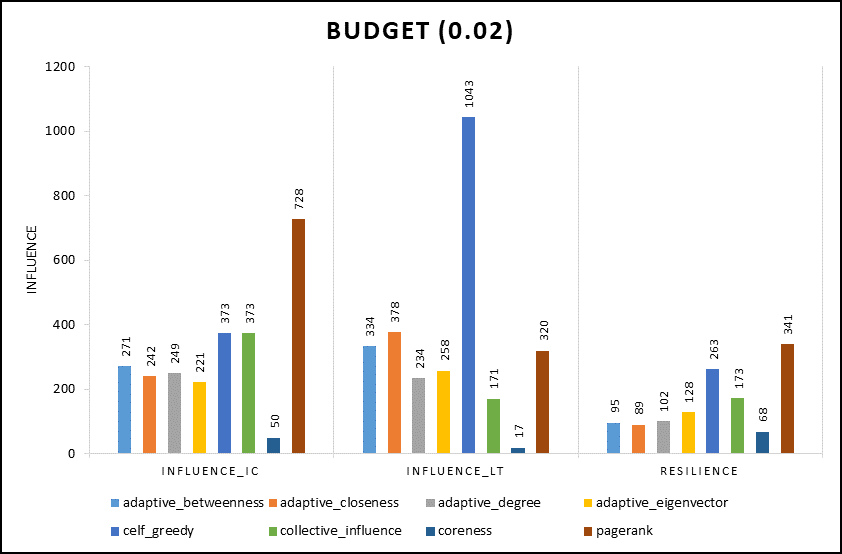
\includegraphics[angle=90, scale=0.65]{fb_tvshows-budget-2}\par 
			\end{multicols}
			\begin{multicols}{2}
				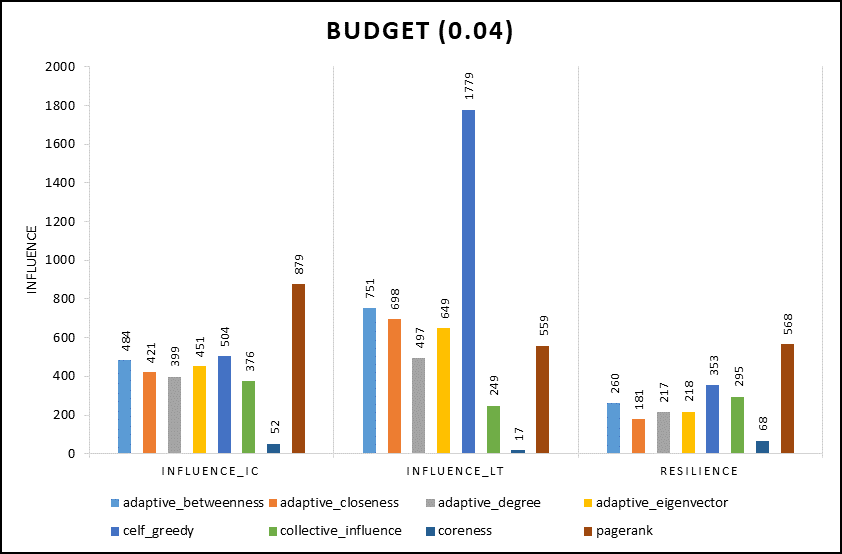
\includegraphics[angle=90, scale=0.65]{fb_tvshows-budget-4}\par 
				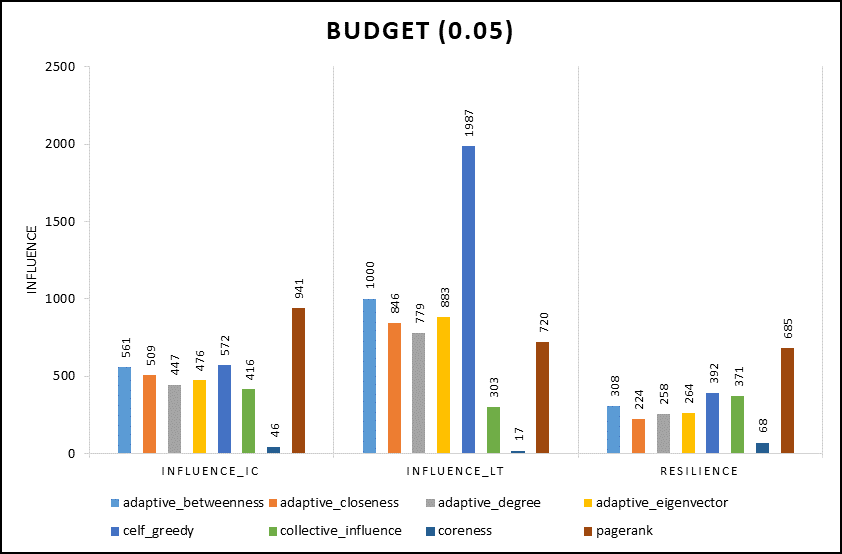
\includegraphics[angle=90, scale=0.65]{fb_tvshows-budget-5}\par 
			\end{multicols}
			
			\caption{Influence measure of Facebook - TV Shows network on range on all budgets evaluated for all three tests.}
			\label{fig:inf-framework-fb_tvshows}
		\end{figure*}
		
		\begin{figure*}[ht]
			\begin{multicols}{2}
				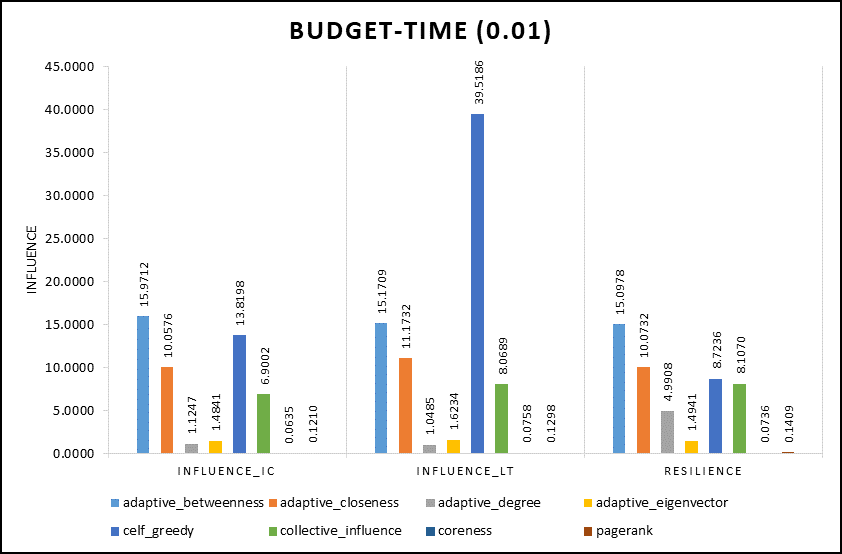
\includegraphics[angle=90, scale=0.65]{fb_tvshows-budget-time-1}\par 
				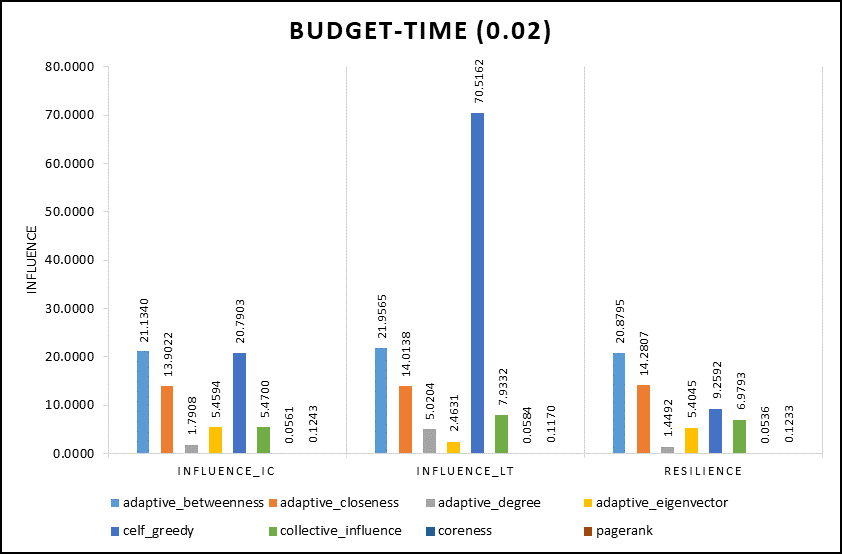
\includegraphics[angle=90, scale=0.65]{fb_tvshows-budget-time-2}\par 
			\end{multicols}
			\begin{multicols}{2}
				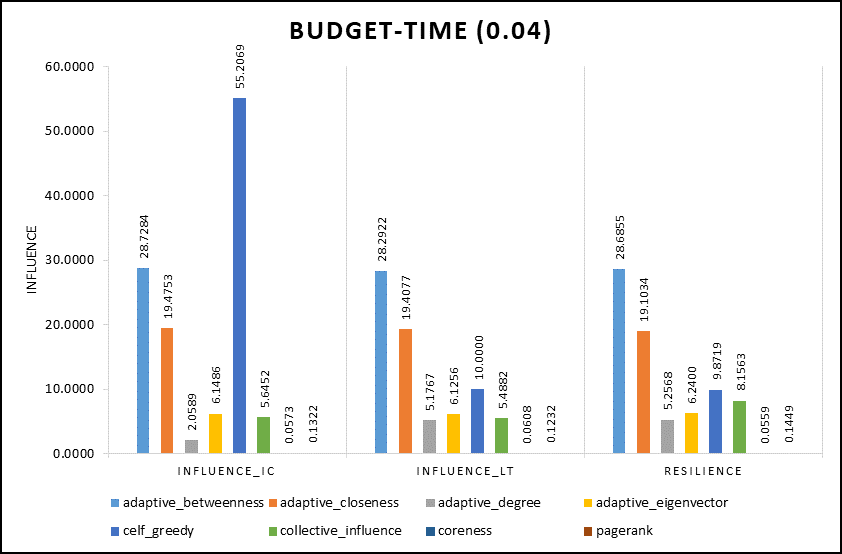
\includegraphics[angle=90, scale=0.65]{fb_tvshows-budget-time-4}\par 
				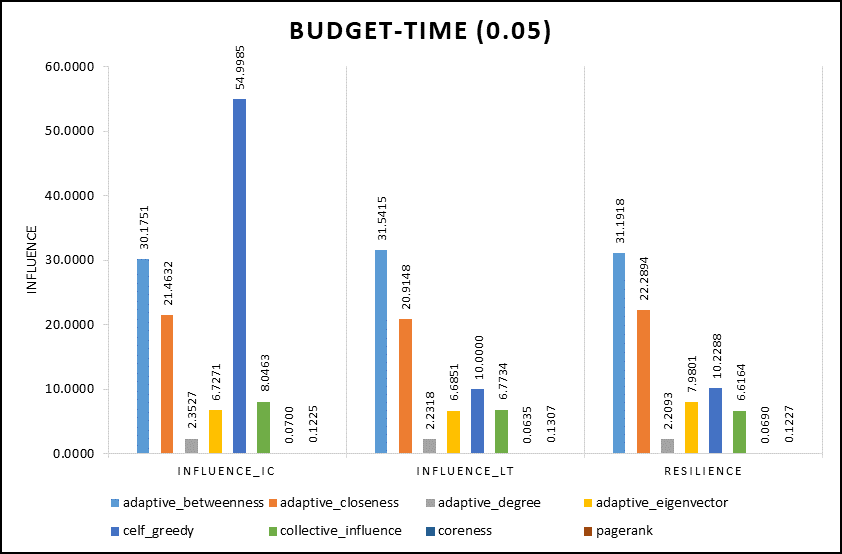
\includegraphics[angle=90, scale=0.65]{fb_tvshows-budget-time-5}\par 
			\end{multicols}
			
			\caption{Normalized elapsed time for budget criteria on Facebook - TV Shows network.}
			\label{fig:inf-framework-fb_tvshows2}
		\end{figure*}
		
		\begin{figure*}[h]
			\begin{multicols}{2}
				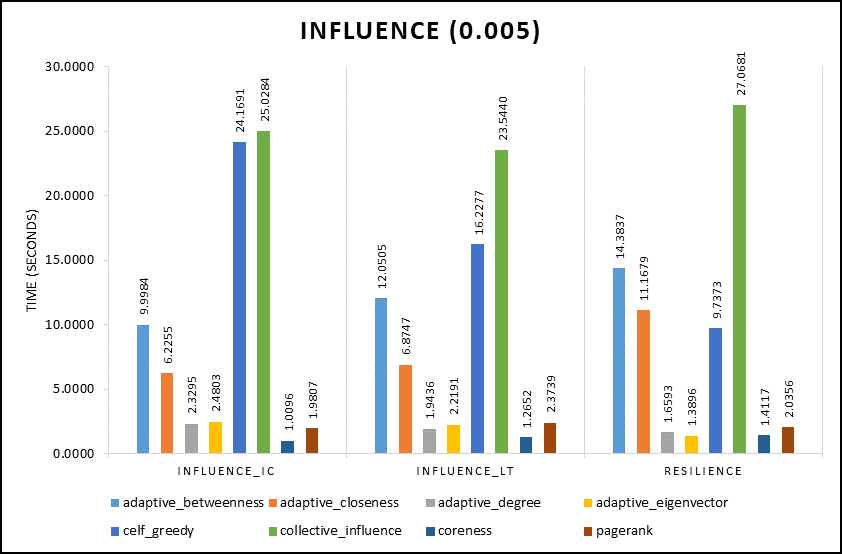
\includegraphics[angle=90, scale=0.65]{fb_tvshows-influence-1}\par 
				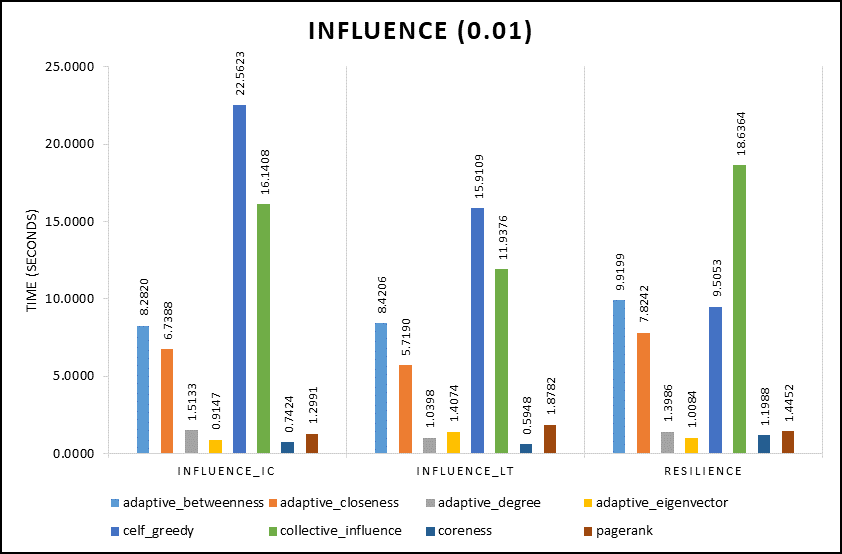
\includegraphics[angle=90, scale=0.65]{fb_tvshows-influence-2}\par 
			\end{multicols}
			\begin{multicols}{2}
				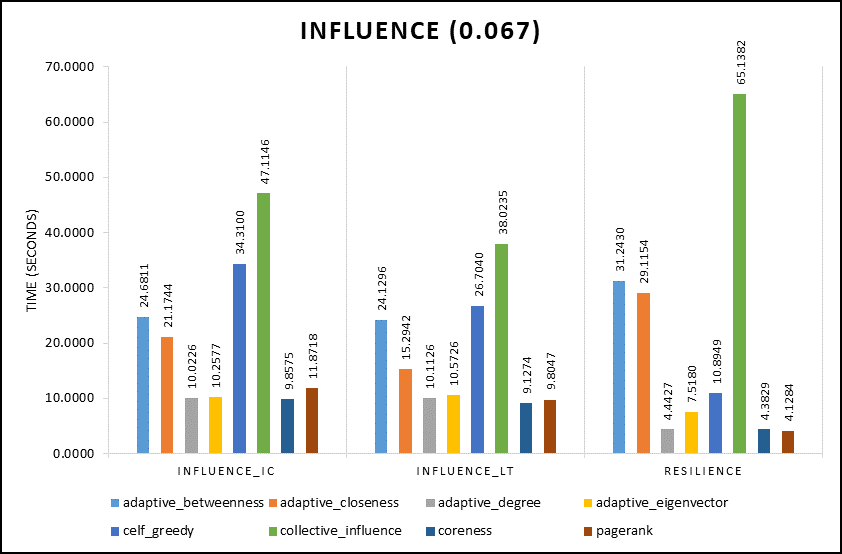
\includegraphics[angle=90, scale=0.65]{fb_tvshows-influence-4}\par 
				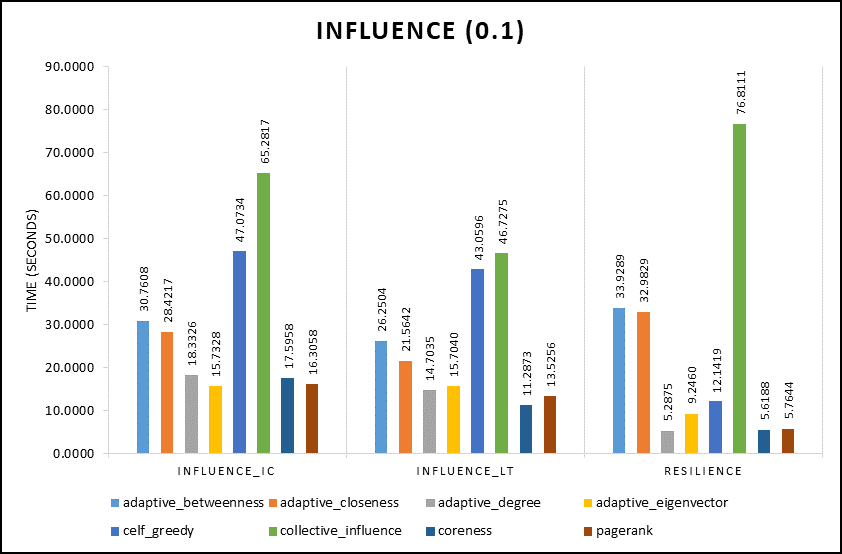
\includegraphics[angle=90, scale=0.65]{fb_tvshows-influence-5}\par 
			\end{multicols}
			
			\caption{Normalized elapsed time for influence criteria on Facebook - TV Shows network.}
			\label{fig:inf-framework-fb_tvshows3}
		\end{figure*}
		
		
		% *** football ***
		\begin{figure*}[ht]
			\begin{multicols}{2}
				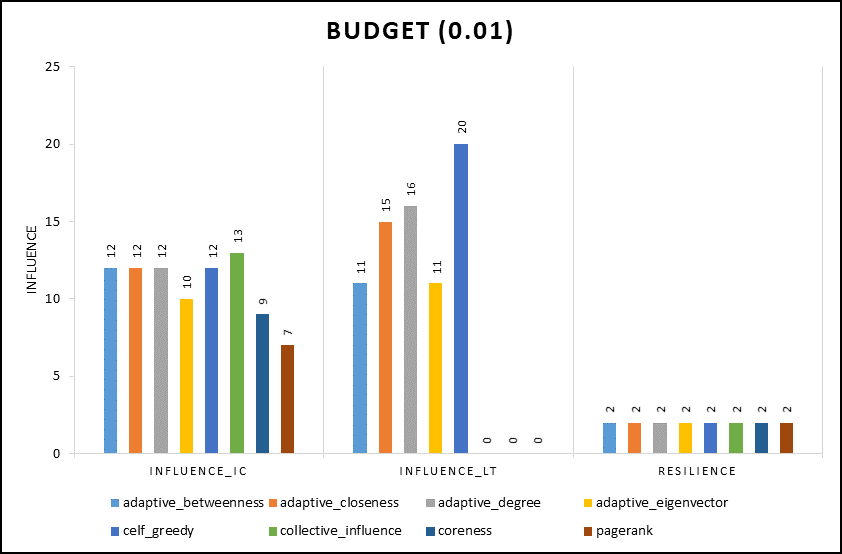
\includegraphics[angle=90, scale=0.65]{football-budget-1}\par 
				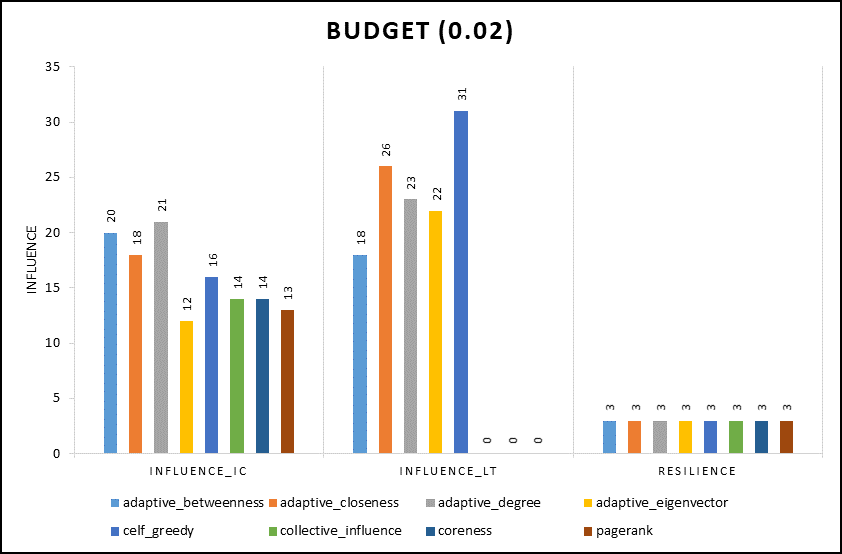
\includegraphics[angle=90, scale=0.65]{football-budget-2}\par 
			\end{multicols}
			\begin{multicols}{2}
				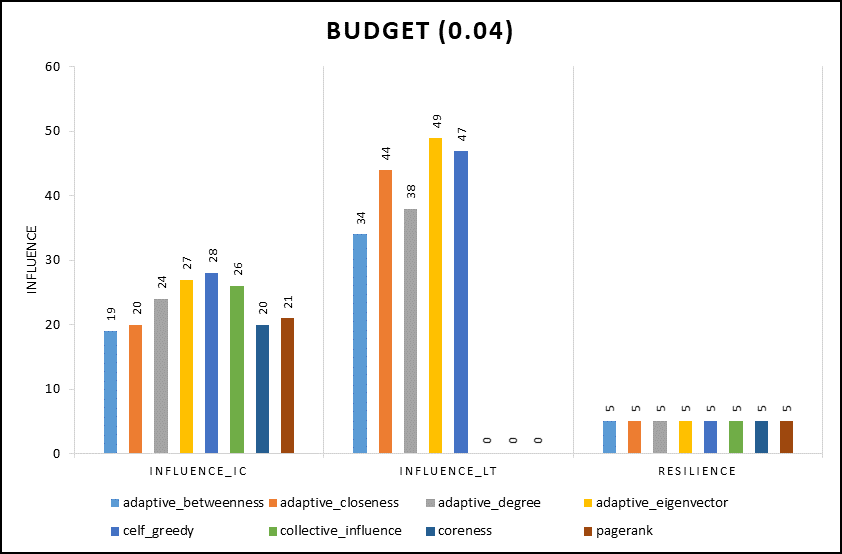
\includegraphics[angle=90, scale=0.65]{football-budget-4}\par 
				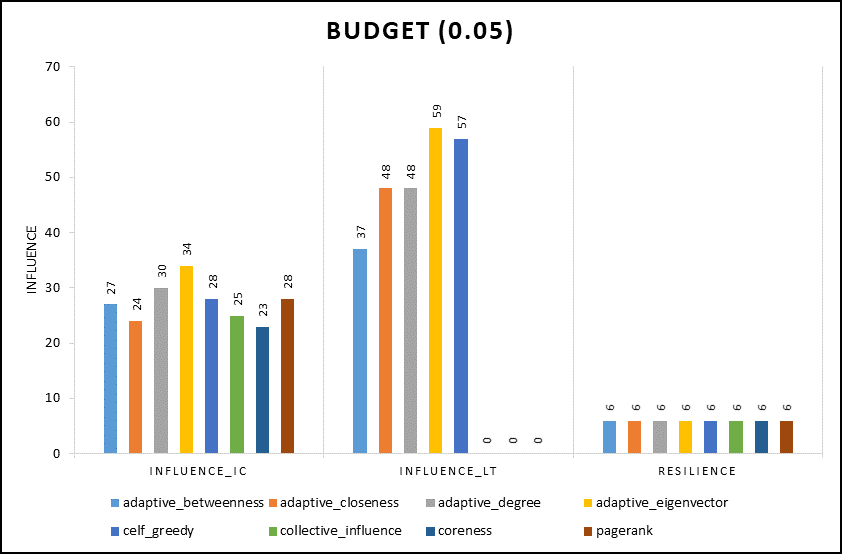
\includegraphics[angle=90, scale=0.65]{football-budget-5}\par 
			\end{multicols}
			
			\caption{Influence measure of Football network on range on all budgets evaluated for all three tests.}
			\label{fig:inf-framework-football}
		\end{figure*}
		
		\begin{figure*}[ht]
			\begin{multicols}{2}
				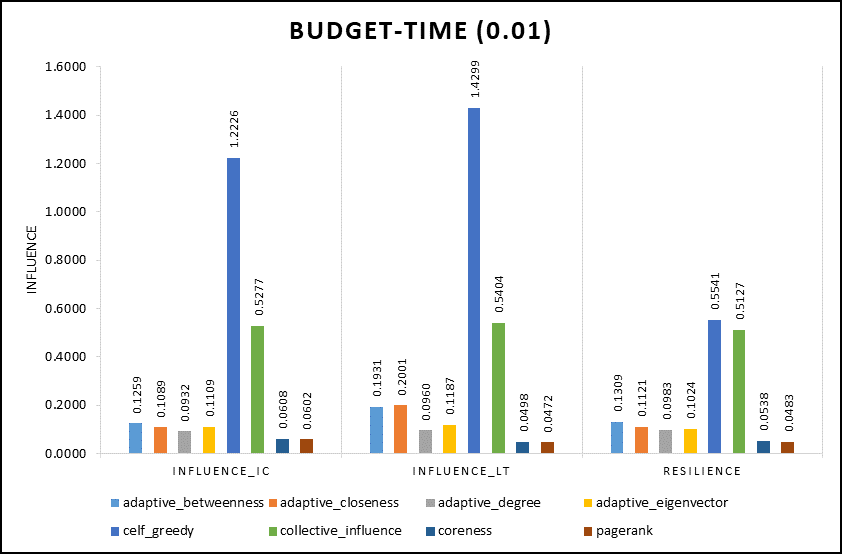
\includegraphics[angle=90, scale=0.65]{football-budget-time-1}\par 
				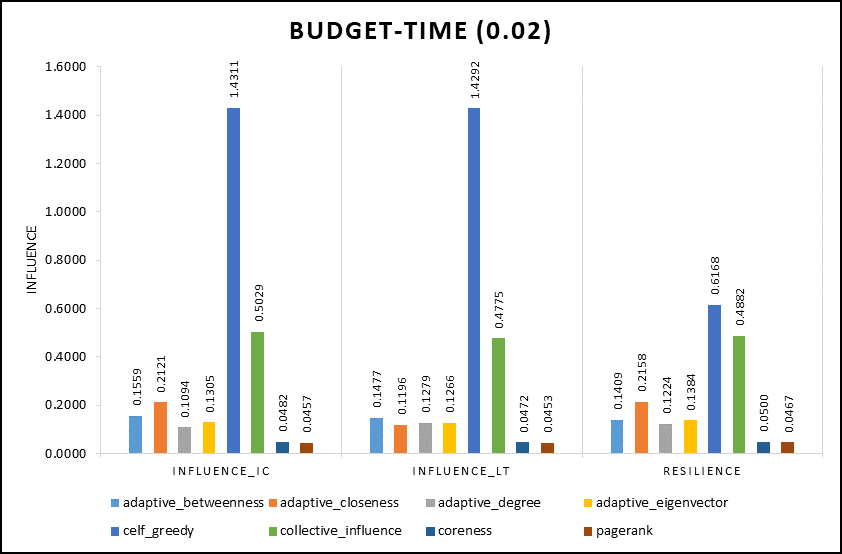
\includegraphics[angle=90, scale=0.65]{football-budget-time-2}\par 
			\end{multicols}
			\begin{multicols}{2}
				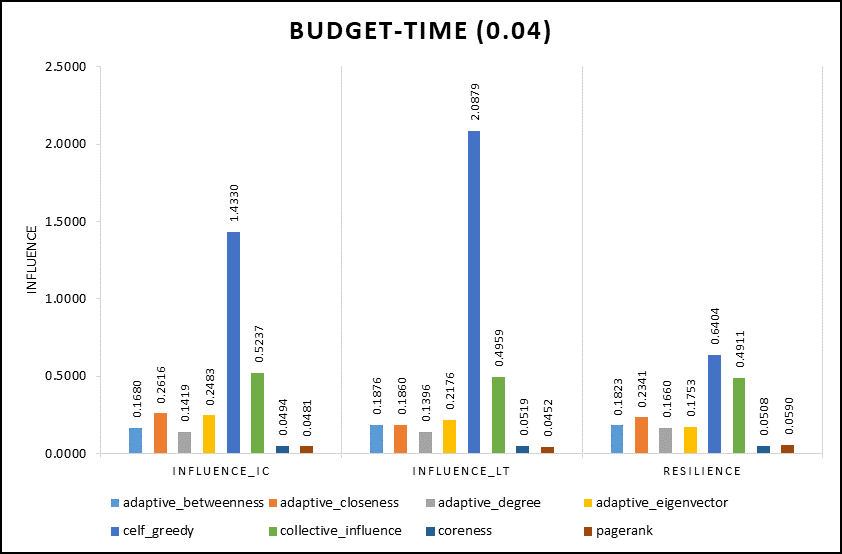
\includegraphics[angle=90, scale=0.65]{football-budget-time-4}\par 
				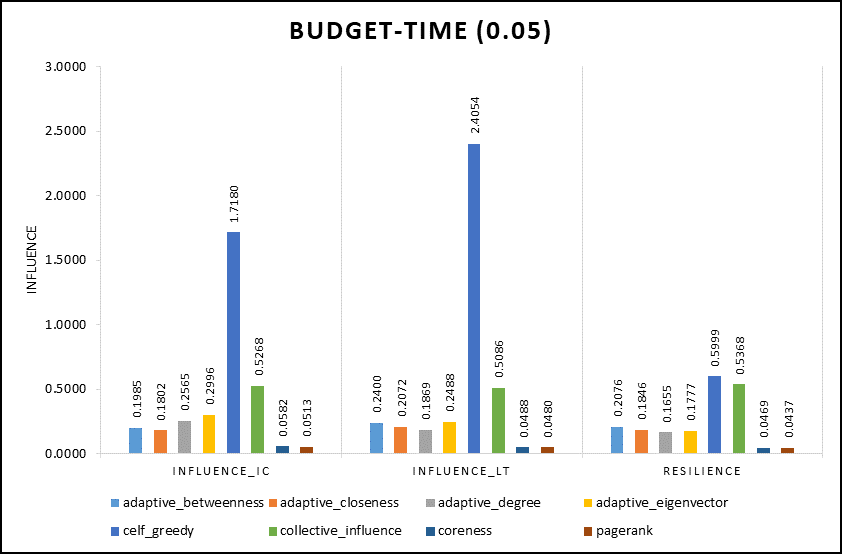
\includegraphics[angle=90, scale=0.65]{football-budget-time-5}\par 
			\end{multicols}
			
			\caption{Normalized elapsed time for budget criteria on Football network.}
			\label{fig:inf-framework-football2}
		\end{figure*}
		
		\begin{figure*}[h]
			\begin{multicols}{2}
				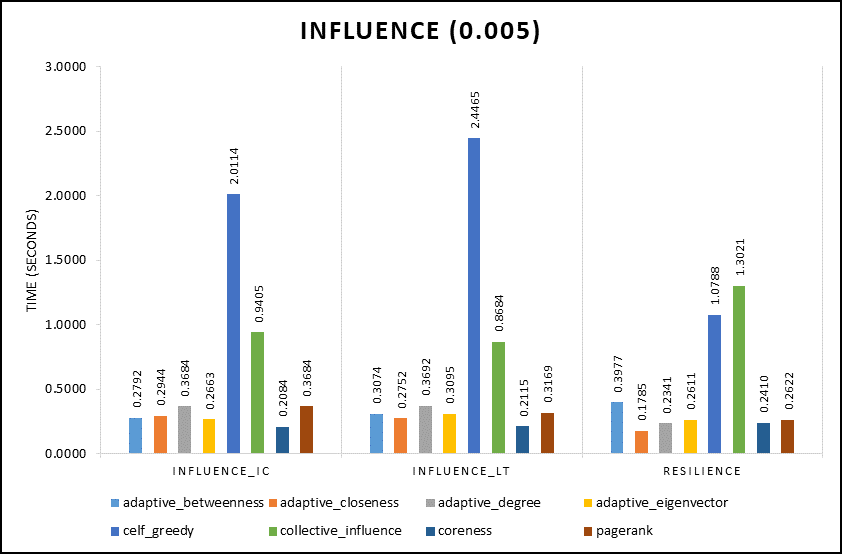
\includegraphics[angle=90, scale=0.65]{football-influence-1}\par 
				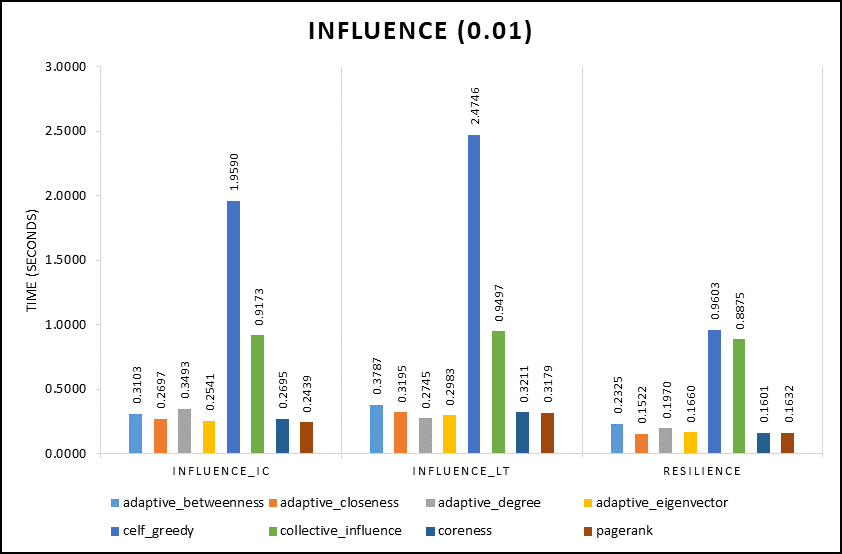
\includegraphics[angle=90, scale=0.65]{football-influence-2}\par 
			\end{multicols}
			\begin{multicols}{2}
				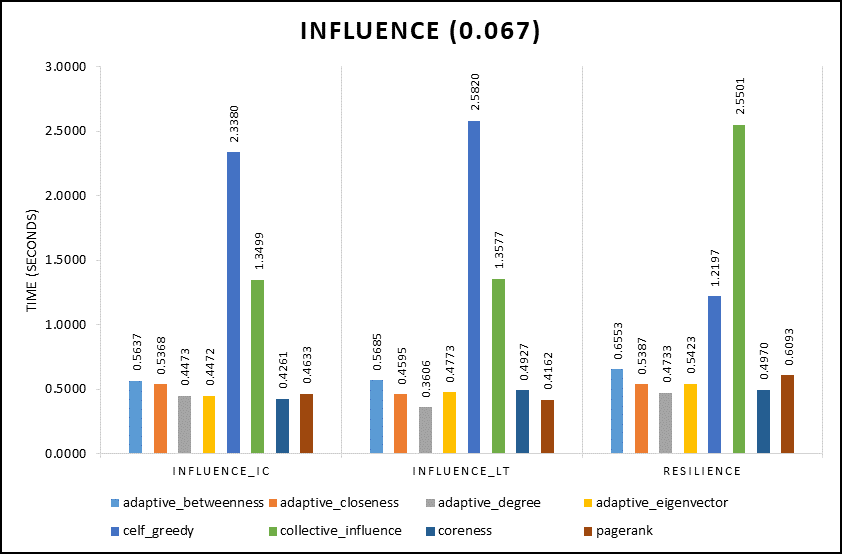
\includegraphics[angle=90, scale=0.65]{football-influence-4}\par 
				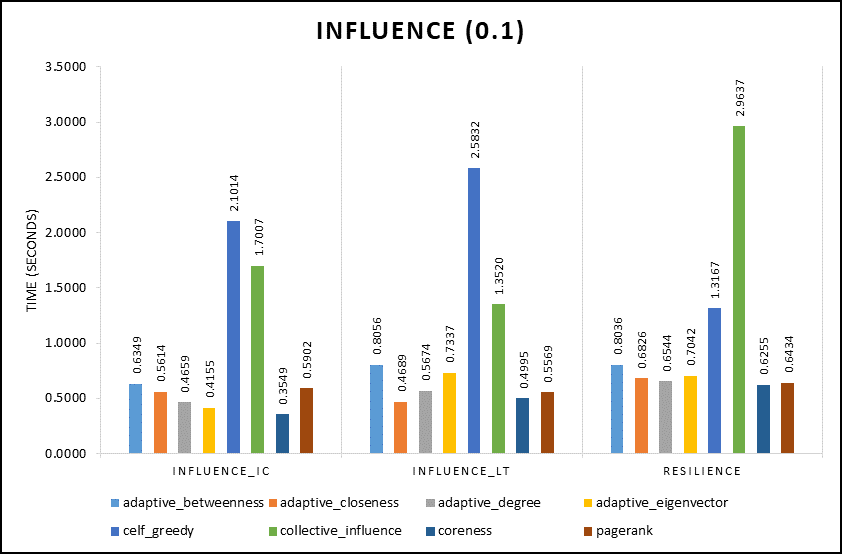
\includegraphics[angle=90, scale=0.65]{football-influence-5}\par 
			\end{multicols}
			
			\caption{Normalized elapsed time for influence criteria on Football network.}
			\label{fig:inf-framework-football3}
		\end{figure*}
		
		
		% *** hamster ***
		\begin{figure*}[ht]
			\begin{multicols}{2}
				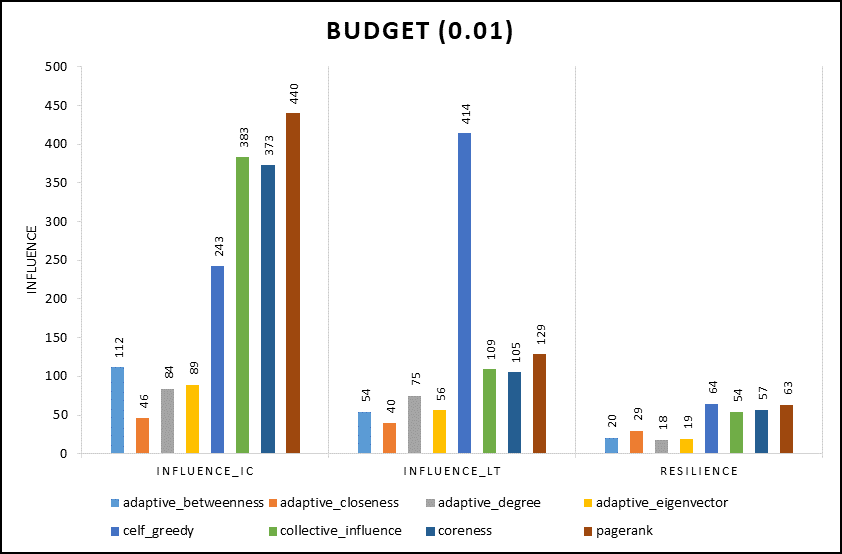
\includegraphics[angle=90, scale=0.65]{hamster-budget-1}\par 
				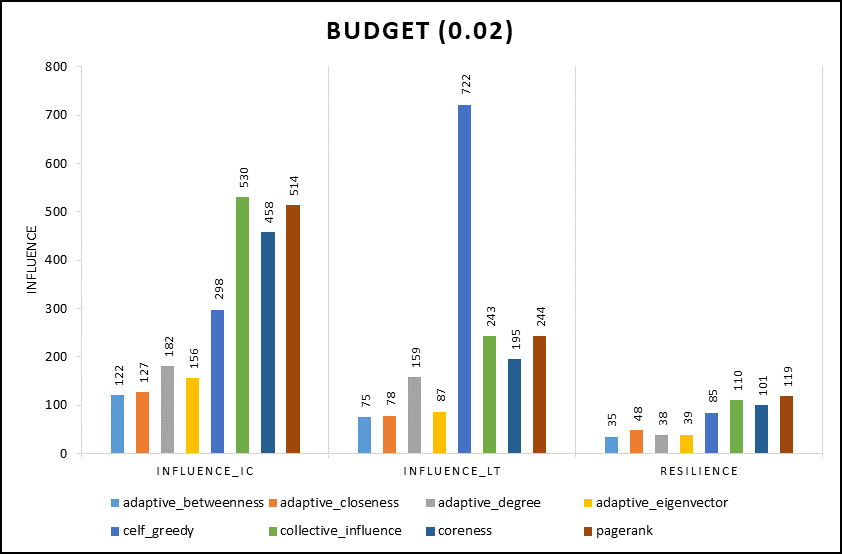
\includegraphics[angle=90, scale=0.65]{hamster-budget-2}\par 
			\end{multicols}
			\begin{multicols}{2}
				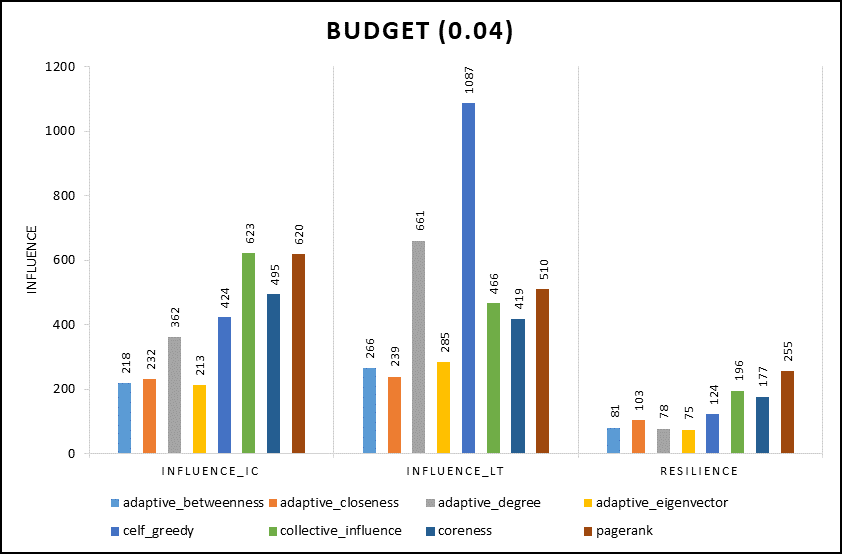
\includegraphics[angle=90, scale=0.65]{hamster-budget-4}\par 
				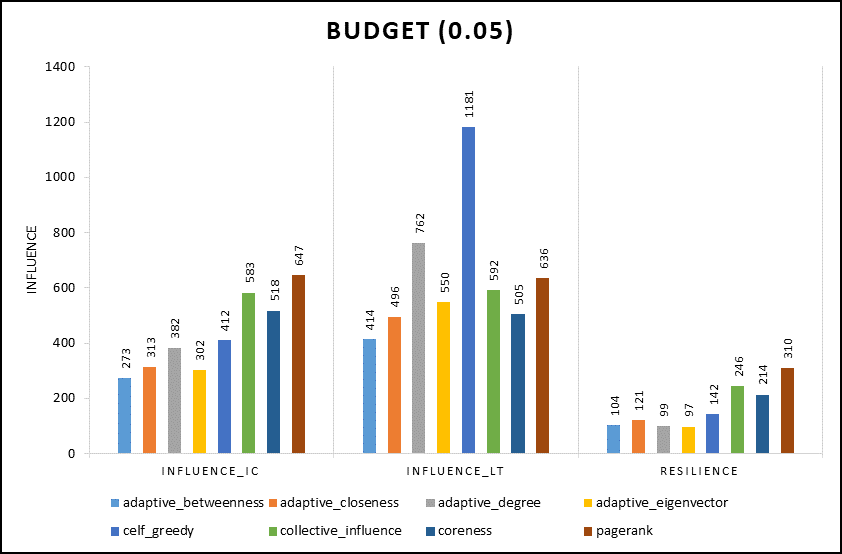
\includegraphics[angle=90, scale=0.65]{hamster-budget-5}\par 
			\end{multicols}
			
			\caption{Influence measure of hamster network on range on all budgets evaluated for all three tests.}
			\label{fig:inf-framework-hamster}
		\end{figure*}
		
		\begin{figure*}[ht]
			\begin{multicols}{2}
				\includegraphics[angle=90, scale=0.65]{hamster-budget-time-1}\par 
				\includegraphics[angle=90, scale=0.65]{hamster-budget-time-2}\par 
			\end{multicols}
			\begin{multicols}{2}
				\includegraphics[angle=90, scale=0.65]{hamster-budget-time-4}\par 
				\includegraphics[angle=90, scale=0.65]{hamster-budget-time-5}\par 
			\end{multicols}
			
			\caption{Normalized elapsed time for budget criteria on hamster network.}
			\label{fig:inf-framework-hamster2}
		\end{figure*}
		
		\begin{figure*}[h]
			\begin{multicols}{2}
				\includegraphics[angle=90, scale=0.65]{hamster-influence-1}\par 
				\includegraphics[angle=90, scale=0.65]{hamster-influence-2}\par 
			\end{multicols}
			\begin{multicols}{2}
				\includegraphics[angle=90, scale=0.65]{hamster-influence-4}\par 
				\includegraphics[angle=90, scale=0.65]{hamster-influence-5}\par 
			\end{multicols}
			
			\caption{Normalized elapsed time for influence criteria on hamster network.}
			\label{fig:inf-framework-hamster3}
		\end{figure*}
		
		
		% *** influence_citation ***
		\begin{figure*}[ht]
			\begin{multicols}{2}
				\includegraphics[angle=90, scale=0.65]{influence_citation-budget-1}\par 
				\includegraphics[angle=90, scale=0.65]{influence_citation-budget-2}\par 
			\end{multicols}
			\begin{multicols}{2}
				\includegraphics[angle=90, scale=0.65]{influence_citation-budget-4}\par 
				\includegraphics[angle=90, scale=0.65]{influence_citation-budget-5}\par 
			\end{multicols}
			
			\caption{Influence measure of Citation network of influence mining papers network on range on all budgets evaluated for all three tests.}
			\label{fig:inf-framework-influence_citation}
		\end{figure*}
		
		\begin{figure*}[ht]
			\begin{multicols}{2}
				\includegraphics[angle=90, scale=0.65]{influence_citation-budget-time-1}\par 
				\includegraphics[angle=90, scale=0.65]{influence_citation-budget-time-2}\par 
			\end{multicols}
			\begin{multicols}{2}
				\includegraphics[angle=90, scale=0.65]{influence_citation-budget-time-4}\par 
				\includegraphics[angle=90, scale=0.65]{influence_citation-budget-time-5}\par 
			\end{multicols}
			
			\caption{Normalized elapsed time for budget criteria on Citation network of influence mining papers.}
			\label{fig:inf-framework-influence_citation2}
		\end{figure*}
		
		\begin{figure*}[h]
			\begin{multicols}{2}
				\includegraphics[angle=90, scale=0.65]{influence_citation-influence-1}\par 
				\includegraphics[angle=90, scale=0.65]{influence_citation-influence-2}\par 
			\end{multicols}
			\begin{multicols}{2}
				\includegraphics[angle=90, scale=0.65]{influence_citation-influence-4}\par 
				\includegraphics[angle=90, scale=0.65]{influence_citation-influence-5}\par 
			\end{multicols}
			
			\caption{Normalized elapsed time for influence criteria on Citation network of influence mining papers.}
			\label{fig:inf-framework-influence_citation3}
		\end{figure*}
		
		
		% *** ita2000 ***
		\begin{figure*}[ht]
			\begin{multicols}{2}
				\includegraphics[angle=90, scale=0.65]{ita2000-budget-1}\par 
				\includegraphics[angle=90, scale=0.65]{ita2000-budget-2}\par 
			\end{multicols}
			\begin{multicols}{2}
				\includegraphics[angle=90, scale=0.65]{ita2000-budget-4}\par 
				\includegraphics[angle=90, scale=0.65]{ita2000-budget-5}\par 
			\end{multicols}
			
			\caption{Influence measure of ITA-2000 network of influence mining papers network on range on all budgets evaluated for all three tests.}
			\label{fig:inf-framework-ita2000}
		\end{figure*}
		
		\begin{figure*}[ht]
			\begin{multicols}{2}
				\includegraphics[angle=90, scale=0.65]{ita2000-budget-time-1}\par 
				\includegraphics[angle=90, scale=0.65]{ita2000-budget-time-2}\par 
			\end{multicols}
			\begin{multicols}{2}
				\includegraphics[angle=90, scale=0.65]{ita2000-budget-time-4}\par 
				\includegraphics[angle=90, scale=0.65]{ita2000-budget-time-5}\par 
			\end{multicols}
			
			\caption{Normalized elapsed time for budget criteria on ITA-2000 network of influence mining papers.}
			\label{fig:inf-framework-ita2000-2}
		\end{figure*}
		
		\begin{figure*}[h]
			\begin{multicols}{2}
				\includegraphics[angle=90, scale=0.65]{ita2000-influence-1}\par 
				\includegraphics[angle=90, scale=0.65]{ita2000-influence-2}\par 
			\end{multicols}
			\begin{multicols}{2}
				\includegraphics[angle=90, scale=0.65]{ita2000-influence-4}\par 
				\includegraphics[angle=90, scale=0.65]{ita2000-influence-5}\par 
			\end{multicols}
			
			\caption{Normalized elapsed time for influence criteria on ITA-2000 network of influence mining papers.}
			\label{fig:inf-framework-ita2000-3}
		\end{figure*}
		
		
		% *** jdk6_dependencies ***
		\begin{figure*}[ht]
			\begin{multicols}{2}
				\includegraphics[angle=90, scale=0.65]{jdk6_dependencies-budget-1}\par 
				\includegraphics[angle=90, scale=0.65]{jdk6_dependencies-budget-2}\par 
			\end{multicols}
			\begin{multicols}{2}
				\includegraphics[angle=90, scale=0.65]{jdk6_dependencies-budget-4}\par 
				\includegraphics[angle=90, scale=0.65]{jdk6_dependencies-budget-5}\par 
			\end{multicols}
			
			\caption{Influence measure of JDK library dependency network of influence mining papers network on range on all budgets evaluated for all three tests.}
			\label{fig:inf-framework-jdk6_dependencies}
		\end{figure*}
		
		\begin{figure*}[ht]
			\begin{multicols}{2}
				\includegraphics[angle=90, scale=0.65]{jdk6_dependencies-budget-time-1}\par 
				\includegraphics[angle=90, scale=0.65]{jdk6_dependencies-budget-time-2}\par 
			\end{multicols}
			\begin{multicols}{2}
				\includegraphics[angle=90, scale=0.65]{jdk6_dependencies-budget-time-4}\par 
				\includegraphics[angle=90, scale=0.65]{jdk6_dependencies-budget-time-5}\par 
			\end{multicols}
			
			\caption{Normalized elapsed time for budget criteria on JDK library dependency network of influence mining papers.}
			\label{fig:inf-framework-jdk6_dependencies2}
		\end{figure*}
		
		\begin{figure*}[h]
			\begin{multicols}{2}
				\includegraphics[angle=90, scale=0.65]{jdk6_dependencies-influence-1}\par 
				\includegraphics[angle=90, scale=0.65]{jdk6_dependencies-influence-2}\par 
			\end{multicols}
			\begin{multicols}{2}
				\includegraphics[angle=90, scale=0.65]{jdk6_dependencies-influence-4}\par 
				\includegraphics[angle=90, scale=0.65]{jdk6_dependencies-influence-5}\par 
			\end{multicols}
			
			\caption{Normalized elapsed time for influence criteria on JDK library dependency network of influence mining papers.}
			\label{fig:inf-framework-jdk6_dependencies3}
		\end{figure*}
		
		
		% *** karate ***
		\begin{figure*}[ht]
			\begin{multicols}{2}
				\includegraphics[angle=90, scale=0.65]{karate-budget-1}\par 
				\includegraphics[angle=90, scale=0.65]{karate-budget-2}\par 
			\end{multicols}
			\begin{multicols}{2}
				\includegraphics[angle=90, scale=0.65]{karate-budget-4}\par 
				\includegraphics[angle=90, scale=0.65]{karate-budget-5}\par 
			\end{multicols}
			
			\caption{Influence measure of Karate network of influence mining papers network on range on all budgets evaluated for all three tests.}
			\label{fig:inf-framework-karate}
		\end{figure*}
		
		\begin{figure*}[ht]
			\begin{multicols}{2}
				\includegraphics[angle=90, scale=0.65]{karate-budget-time-1}\par 
				\includegraphics[angle=90, scale=0.65]{karate-budget-time-2}\par 
			\end{multicols}
			\begin{multicols}{2}
				\includegraphics[angle=90, scale=0.65]{karate-budget-time-4}\par 
				\includegraphics[angle=90, scale=0.65]{karate-budget-time-5}\par 
			\end{multicols}
			
			\caption{Normalized elapsed time for budget criteria on Karate network of influence mining papers.}
			\label{fig:inf-framework-karate2}
		\end{figure*}
		
		\begin{figure*}[h]
			\begin{multicols}{2}
				\includegraphics[angle=90, scale=0.65]{karate-influence-1}\par 
				\includegraphics[angle=90, scale=0.65]{karate-influence-2}\par 
			\end{multicols}
			\begin{multicols}{2}
				\includegraphics[angle=90, scale=0.65]{karate-influence-4}\par 
				\includegraphics[angle=90, scale=0.65]{karate-influence-5}\par 
			\end{multicols}
			
			\caption{Normalized elapsed time for influence criteria on Karate network of influence mining papers.}
			\label{fig:inf-framework-karate3}
		\end{figure*}
		
		%%!TEX root = ../appendix-C2.tex
%% ******************************* Thesis Appendix C: Figures ****************************

	% *** linux_code ***
	\begin{figure*}[ht]
		\begin{multicols}{2}
			\includegraphics[angle=90, scale=0.65]{linux_code-budget-1}\par 
			\includegraphics[angle=90, scale=0.65]{linux_code-budget-time-1}\par 
		\end{multicols}
		\begin{multicols}{2}
			\includegraphics[angle=90, scale=0.65]{linux_code-influence-1}\par 
		\end{multicols}
		
		\caption{Influence measure (top-left), normalized elapsed time for budget criteria (top-right), and normalized elapsed time for influence criteria (bottom-left) of Linux network.}
		\label{fig:inf-framework-linux_code}
	\end{figure*}

	
	% *** moreno ***
	\begin{figure*}[ht]
		\begin{multicols}{2}
			\includegraphics[angle=90, scale=0.65]{moreno-budget-1}\par 
			\includegraphics[angle=90, scale=0.65]{moreno-budget-2}\par 
		\end{multicols}
		\begin{multicols}{2}
			\includegraphics[angle=90, scale=0.65]{moreno-budget-4}\par 
			\includegraphics[angle=90, scale=0.65]{moreno-budget-5}\par 
		\end{multicols}
		
		\caption{Influence measure of Moreno network of influence mining papers network on range on all budgets evaluated for all three tests.}
		\label{fig:inf-framework-moreno}
	\end{figure*}
	
	\begin{figure*}[ht]
		\begin{multicols}{2}
			\includegraphics[angle=90, scale=0.65]{moreno-budget-time-1}\par 
			\includegraphics[angle=90, scale=0.65]{moreno-budget-time-2}\par 
		\end{multicols}
		\begin{multicols}{2}
			\includegraphics[angle=90, scale=0.65]{moreno-budget-time-4}\par 
			\includegraphics[angle=90, scale=0.65]{moreno-budget-time-5}\par 
		\end{multicols}
		
		\caption{Normalized elapsed time for budget criteria on Moreno network of influence mining papers.}
		\label{fig:inf-framework-moreno2}
	\end{figure*}
	
	\begin{figure*}[h]
		\begin{multicols}{2}
			\includegraphics[angle=90, scale=0.65]{moreno-influence-1}\par 
			\includegraphics[angle=90, scale=0.65]{moreno-influence-2}\par 
		\end{multicols}
		\begin{multicols}{2}
			\includegraphics[angle=90, scale=0.65]{moreno-influence-4}\par 
			\includegraphics[angle=90, scale=0.65]{moreno-influence-5}\par 
		\end{multicols}
		
		\caption{Normalized elapsed time for influence criteria on Moreno network of influence mining papers.}
		\label{fig:inf-framework-moreno3}
	\end{figure*}
	
	
	% *** nematode ***
	\begin{figure*}[ht]
		\begin{multicols}{2}
			\includegraphics[angle=90, scale=0.65]{nematode-budget-1}\par 
			\includegraphics[angle=90, scale=0.65]{nematode-budget-2}\par 
		\end{multicols}
		\begin{multicols}{2}
			\includegraphics[angle=90, scale=0.65]{nematode-budget-4}\par 
			\includegraphics[angle=90, scale=0.65]{nematode-budget-5}\par 
		\end{multicols}
		
		\caption{Influence measure of Nematode network of influence mining papers network on range on all budgets evaluated for all three tests.}
		\label{fig:inf-framework-nematode}
	\end{figure*}
	
	\begin{figure*}[ht]
		\begin{multicols}{2}
			\includegraphics[angle=90, scale=0.65]{nematode-budget-time-1}\par 
			\includegraphics[angle=90, scale=0.65]{nematode-budget-time-2}\par 
		\end{multicols}
		\begin{multicols}{2}
			\includegraphics[angle=90, scale=0.65]{nematode-budget-time-4}\par 
			\includegraphics[angle=90, scale=0.65]{nematode-budget-time-5}\par 
		\end{multicols}
		
		\caption{Normalized elapsed time for budget criteria on Nematode network of influence mining papers.}
		\label{fig:inf-framework-nematode2}
	\end{figure*}
	
	\begin{figure*}[h]
		\begin{multicols}{2}
			\includegraphics[angle=90, scale=0.65]{nematode-influence-1}\par 
			\includegraphics[angle=90, scale=0.65]{nematode-influence-2}\par 
		\end{multicols}
		\begin{multicols}{2}
			\includegraphics[angle=90, scale=0.65]{nematode-influence-4}\par 
			\includegraphics[angle=90, scale=0.65]{nematode-influence-5}\par 
		\end{multicols}
		
		\caption{Normalized elapsed time for influence criteria on Nematode network of influence mining papers.}
		\label{fig:inf-framework-nematode3}
	\end{figure*}
	
	
	% *** political_blog ***
	\begin{figure*}[ht]
		\begin{multicols}{2}
			\includegraphics[angle=90, scale=0.65]{political_blog-budget-1}\par 
			\includegraphics[angle=90, scale=0.65]{political_blog-budget-2}\par 
		\end{multicols}
		\begin{multicols}{2}
			\includegraphics[angle=90, scale=0.65]{political_blog-budget-4}\par 
			\includegraphics[angle=90, scale=0.65]{political_blog-budget-5}\par 
		\end{multicols}
		
		\caption{Influence measure of political blog network of influence mining papers network on range on all budgets evaluated for all three tests.}
		\label{fig:inf-framework-political_blog}
	\end{figure*}
	
	\begin{figure*}[ht]
		\begin{multicols}{2}
			\includegraphics[angle=90, scale=0.65]{political_blog-budget-time-1}\par 
			\includegraphics[angle=90, scale=0.65]{political_blog-budget-time-2}\par 
		\end{multicols}
		\begin{multicols}{2}
			\includegraphics[angle=90, scale=0.65]{political_blog-budget-time-4}\par 
			\includegraphics[angle=90, scale=0.65]{political_blog-budget-time-5}\par 
		\end{multicols}
		
		\caption{Normalized elapsed time for budget criteria on political blog network of influence mining papers.}
		\label{fig:inf-framework-political_blog2}
	\end{figure*}
	
	\begin{figure*}[h]
		\begin{multicols}{2}
			\includegraphics[angle=90, scale=0.65]{political_blog-influence-1}\par 
			\includegraphics[angle=90, scale=0.65]{political_blog-influence-2}\par 
		\end{multicols}
		\begin{multicols}{2}
			\includegraphics[angle=90, scale=0.65]{political_blog-influence-4}\par 
			\includegraphics[angle=90, scale=0.65]{political_blog-influence-5}\par 
		\end{multicols}
		
		\caption{Normalized elapsed time for influence criteria on political blog network of influence mining papers.}
		\label{fig:inf-framework-political_blog3}
	\end{figure*}
	
	
	% *** protein ***
	\begin{figure*}[ht]
		\begin{multicols}{2}
			\includegraphics[angle=90, scale=0.65]{protein-budget-1}\par 
			\includegraphics[angle=90, scale=0.65]{protein-budget-2}\par 
		\end{multicols}
		\begin{multicols}{2}
			\includegraphics[angle=90, scale=0.65]{protein-budget-4}\par 
			\includegraphics[angle=90, scale=0.65]{protein-budget-5}\par 
		\end{multicols}
		
		\caption{Influence measure of protein network of influence mining papers network on range on all budgets evaluated for all three tests.}
		\label{fig:inf-framework-protein}
	\end{figure*}
	
	\begin{figure*}[ht]
		\begin{multicols}{2}
			\includegraphics[angle=90, scale=0.65]{protein-budget-time-1}\par 
			\includegraphics[angle=90, scale=0.65]{protein-budget-time-2}\par 
		\end{multicols}
		\begin{multicols}{2}
			\includegraphics[angle=90, scale=0.65]{protein-budget-time-4}\par 
			\includegraphics[angle=90, scale=0.65]{protein-budget-time-5}\par 
		\end{multicols}
		
		\caption{Normalized elapsed time for budget criteria on protein network of influence mining papers.}
		\label{fig:inf-framework-protein2}
	\end{figure*}
	
	\begin{figure*}[h]
		\begin{multicols}{2}
			\includegraphics[angle=90, scale=0.65]{protein-influence-1}\par 
			\includegraphics[angle=90, scale=0.65]{protein-influence-2}\par 
		\end{multicols}
		\begin{multicols}{2}
			\includegraphics[angle=90, scale=0.65]{protein-influence-4}\par 
			\includegraphics[angle=90, scale=0.65]{protein-influence-5}\par 
		\end{multicols}
		
		\caption{Normalized elapsed time for influence criteria on protein network of influence mining papers.}
		\label{fig:inf-framework-protein3}
	\end{figure*}
	
	
	% *** tech_routers ***
	\begin{figure*}[ht]
		\begin{multicols}{2}
			\includegraphics[angle=90, scale=0.65]{tech_routers-budget-1}\par 
			\includegraphics[angle=90, scale=0.65]{tech_routers-budget-2}\par 
		\end{multicols}
		\begin{multicols}{2}
			\includegraphics[angle=90, scale=0.65]{tech_routers-budget-4}\par 
			\includegraphics[angle=90, scale=0.65]{tech_routers-budget-5}\par 
		\end{multicols}
		
		\caption{Influence measure of Tech routers network of influence mining papers network on range on all budgets evaluated for all three tests.}
		\label{fig:inf-framework-tech_routers}
	\end{figure*}
	
	\begin{figure*}[ht]
		\begin{multicols}{2}
			\includegraphics[angle=90, scale=0.65]{tech_routers-budget-time-1}\par 
			\includegraphics[angle=90, scale=0.65]{tech_routers-budget-time-2}\par 
		\end{multicols}
		\begin{multicols}{2}
			\includegraphics[angle=90, scale=0.65]{tech_routers-budget-time-4}\par 
			\includegraphics[angle=90, scale=0.65]{tech_routers-budget-time-5}\par 
		\end{multicols}
		
		\caption{Normalized elapsed time for budget criteria on Tech routers network of influence mining papers.}
		\label{fig:inf-framework-tech_routers2}
	\end{figure*}
	
	\begin{figure*}[h]
		\begin{multicols}{2}
			\includegraphics[angle=90, scale=0.65]{tech_routers-influence-1}\par 
			\includegraphics[angle=90, scale=0.65]{tech_routers-influence-2}\par 
		\end{multicols}
		\begin{multicols}{2}
			\includegraphics[angle=90, scale=0.65]{tech_routers-influence-4}\par 
			\includegraphics[angle=90, scale=0.65]{tech_routers-influence-5}\par 
		\end{multicols}
		
		\caption{Normalized elapsed time for influence criteria on Tech routers network of influence mining papers.}
		\label{fig:inf-framework-tech_routers3}
	\end{figure*}
	
	
	% *** usairport ***
	\begin{figure*}[ht]
		\begin{multicols}{2}
			\includegraphics[angle=90, scale=0.65]{usairport-budget-1}\par 
			\includegraphics[angle=90, scale=0.65]{usairport-budget-2}\par 
		\end{multicols}
		\begin{multicols}{2}
			\includegraphics[angle=90, scale=0.65]{usairport-budget-4}\par 
			\includegraphics[angle=90, scale=0.65]{usairport-budget-5}\par 
		\end{multicols}
		
		\caption{Influence measure of US Airport network of influence mining papers network on range on all budgets evaluated for all three tests.}
		\label{fig:inf-framework-usairport}
	\end{figure*}
	
	\begin{figure*}[ht]
		\begin{multicols}{2}
			\includegraphics[angle=90, scale=0.65]{usairport-budget-time-1}\par 
			\includegraphics[angle=90, scale=0.65]{usairport-budget-time-2}\par 
		\end{multicols}
		\begin{multicols}{2}
			\includegraphics[angle=90, scale=0.65]{usairport-budget-time-4}\par 
			\includegraphics[angle=90, scale=0.65]{usairport-budget-time-5}\par 
		\end{multicols}
		
		\caption{Normalized elapsed time for budget criteria on US Airport network of influence mining papers.}
		\label{fig:inf-framework-usairport2}
	\end{figure*}
	
	\begin{figure*}[h]
		\begin{multicols}{2}
			\includegraphics[angle=90, scale=0.65]{usairport-influence-1}\par 
			\includegraphics[angle=90, scale=0.65]{usairport-influence-2}\par 
		\end{multicols}
		\begin{multicols}{2}
			\includegraphics[angle=90, scale=0.65]{usairport-influence-4}\par 
			\includegraphics[angle=90, scale=0.65]{usairport-influence-5}\par 
		\end{multicols}
		
		\caption{Normalized elapsed time for influence criteria on US Airport network of influence mining papers.}
		\label{fig:inf-framework-usairport3}
	\end{figure*}
	
	
	% *** web_spam ***
	\begin{figure*}[ht]
		\begin{multicols}{2}
			\includegraphics[angle=90, scale=0.65]{web_spam-budget-1}\par 
			\includegraphics[angle=90, scale=0.65]{web_spam-budget-2}\par 
		\end{multicols}
		\begin{multicols}{2}
			\includegraphics[angle=90, scale=0.65]{web_spam-budget-4}\par 
			\includegraphics[angle=90, scale=0.65]{web_spam-budget-5}\par 
		\end{multicols}
		
		\caption{Influence measure of Web Spam network of influence mining papers network on range on all budgets evaluated for all three tests.}
		\label{fig:inf-framework-web_spam}
	\end{figure*}
	
	\begin{figure*}[ht]
		\begin{multicols}{2}
			\includegraphics[angle=90, scale=0.65]{web_spam-budget-time-1}\par 
			\includegraphics[angle=90, scale=0.65]{web_spam-budget-time-2}\par 
		\end{multicols}
		\begin{multicols}{2}
			\includegraphics[angle=90, scale=0.65]{web_spam-budget-time-4}\par 
			\includegraphics[angle=90, scale=0.65]{web_spam-budget-time-5}\par 
		\end{multicols}
		
		\caption{Normalized elapsed time for budget criteria on Web Spam network of influence mining papers.}
		\label{fig:inf-framework-web_spam2}
	\end{figure*}
	
	\begin{figure*}[h]
		\begin{multicols}{2}
			\includegraphics[angle=90, scale=0.65]{web_spam-influence-1}\par 
			\includegraphics[angle=90, scale=0.65]{web_spam-influence-2}\par 
		\end{multicols}
		\begin{multicols}{2}
			\includegraphics[angle=90, scale=0.65]{web_spam-influence-4}\par 
			\includegraphics[angle=90, scale=0.65]{web_spam-influence-5}\par 
		\end{multicols}
		
		\caption{Normalized elapsed time for influence criteria on Web Spam network of influence mining papers.}
		\label{fig:inf-framework-web_spam3}
	\end{figure*}
	
	
	% *** world_trade ***
	\begin{figure*}[ht]
		\begin{multicols}{2}
			\includegraphics[angle=90, scale=0.65]{world_trade-budget-1}\par 
			\includegraphics[angle=90, scale=0.65]{world_trade-budget-2}\par 
		\end{multicols}
		\begin{multicols}{2}
			\includegraphics[angle=90, scale=0.65]{world_trade-budget-4}\par 
			\includegraphics[angle=90, scale=0.65]{world_trade-budget-5}\par 
		\end{multicols}
		
		\caption{Influence measure of World trade network of influence mining papers network on range on all budgets evaluated for all three tests.}
		\label{fig:inf-framework-world_trade}
	\end{figure*}
	
	\begin{figure*}[ht]
		\begin{multicols}{2}
			\includegraphics[angle=90, scale=0.65]{world_trade-budget-time-1}\par 
			\includegraphics[angle=90, scale=0.65]{world_trade-budget-time-2}\par 
		\end{multicols}
		\begin{multicols}{2}
			\includegraphics[angle=90, scale=0.65]{world_trade-budget-time-4}\par 
			\includegraphics[angle=90, scale=0.65]{world_trade-budget-time-5}\par 
		\end{multicols}
		
		\caption{Normalized elapsed time for budget criteria on World trade network of influence mining papers.}
		\label{fig:inf-framework-world_trade2}
	\end{figure*}
	
	\begin{figure*}[h]
		\begin{multicols}{2}
			\includegraphics[angle=90, scale=0.65]{world_trade-influence-1}\par 
			\includegraphics[angle=90, scale=0.65]{world_trade-influence-2}\par 
		\end{multicols}
		\begin{multicols}{2}
			\includegraphics[angle=90, scale=0.65]{world_trade-influence-4}\par 
			\includegraphics[angle=90, scale=0.65]{world_trade-influence-5}\par 
		\end{multicols}
		
		\caption{Normalized elapsed time for influence criteria on World trade network of influence mining papers.}
		\label{fig:inf-framework-world_trade3}
	\end{figure*}


	\end{appendices}
	
	% *************************************** Index ********************************
	\printthesisindex % If index is present
	
\end{document}


%TODO: refer the figures to the right subsections like (see figure 1.14 - 1.28) wherever applicable